\documentclass[10pt,a4wide,twoside]{book}

\usepackage[pdfborder={0 0 0 }]{hyperref}
\usepackage{enumerate}
\usepackage{feynmf}
\usepackage{rotating}
\usepackage{pdflscape}
\usepackage{subfigure}
\usepackage{placeins}
\usepackage{algorithmicx}
\usepackage{algpseudocode}
\usepackage{algorithm}
\usepackage{multirow}
\usepackage{refcount}
\usepackage{emptypage}
%\usepackage[linesnumbered,ruled,vlined]{algorithm2e}



\usepackage{chapterbib}
\usepackage{verbatim}
\usepackage{listings}
\usepackage{graphicx}
\usepackage{epic}
\usepackage{eepic}
\usepackage{a4wide}
\usepackage{color}
\usepackage{amsmath}
\usepackage{amssymb}
\usepackage[dvips]{epsfig}
\usepackage[T1]{fontenc}
\usepackage{cite} % [2,3,4] --> [2--4]
\usepackage{shadow}
\usepackage{hyperref}
\usepackage{parskip}
\usepackage{lscape}
\usepackage{tikz}
%\usetikzlibrary{shapes,arrows}
\usepackage{pstricks}
%\usepackage{pst-add}
%\usepackage{pst-node}
%\usepackage{pst-blur}
%\usepackage{axodraw4j}
\usepackage{simplewick}
\usepackage[small,bf]{caption}
\usepackage{xcolor}
\usepackage{textcomp}
\usepackage{listings}
\usepackage{color}
\usepackage{exercise}





\setcounter{tocdepth}{2}

\lstset{language=c++}
\lstset{alsolanguage=[90]Fortran}
\lstset{basicstyle=\small}
\lstset{backgroundcolor=\color{white}}
\lstset{frame=single}
\lstset{stringstyle=\ttfamily}
\lstset{keywordstyle=\color{red}\bfseries}
\lstset{commentstyle=\itshape\color{blue}}
\lstset{showspaces=false}
\lstset{showstringspaces=false}
\lstset{showtabs=false}
\lstset{breaklines}

\newcommand{\OP}[1]{{\bf\widehat{#1}}}
\newcommand{\be}{\begin{equation}}
\newcommand{\ee}{\end{equation}}
\newcommand{\normord}[1]{
    \left\{#1\right\}
}

\newcommand{\braket}[2]
        {\langle #1 | #2 \rangle}
\newcommand{\ket}[1]
        {|#1\rangle}
\newcommand{\bra}[1]
        {\langle #1 |}
\newcommand{\element}[3]
        {\bra{#1}#2\ket{#3}}

\newcommand*{\indre}[2]{\langle#1|#2\rangle}
\newcommand*{\for}[3]{\langle#1|#2|#3\rangle}
\newcommand*{\forS}[3]{\left<#1\left|#2\right|#3\right>}
\newcommand*{\forsmall}[3]{<#1|#2|#3>}
\newcommand*{\absk}[1]{\left|#1\right|^2}
\newcommand*{\abs}[1]{\left|#1\right|}
\newcommand*{\vek}[1]{\mathbf{#1}}
\newcommand*{\pr}[1]{\left(#1\right)}
\newcommand*{\fpr}[1]{\left[#1\right]}
\newcommand*{\kpr}[1]{\left\{#1\right\}}
\newcommand*{\forv}[1]{\langle#1\rangle}
\newcommand*{\pder}[2]{\frac{\partial#1}{\partial#2}}
\newcommand*{\der}[2]{\frac{d#1}{d#2}}
\newcommand*{\rmn}[1]{\mathrm{#1}}
\newcommand*{\dg}{\dagger}
\newcommand*{\calH}{\mathcal{H}}
\newcommand*{\n}{\vek{n}}
\newcommand*{\svek}{\boldsymbol{\sigma}}
\newcommand*{\Svek}{\mathbf{S}}
\newcommand*{\ssvek}{\boldsymbol{\Sigma}}
\newcommand*{\en}{\mathbf{1}}
\newcommand*{\matr}[1]{\begin{pmatrix}#1\end{pmatrix}}
\newcommand*{\cre}[1]{a^{\dagger}_{#1}}
\newcommand*{\an}[1]{a_{#1}}
\newcommand*{\crequasi}[1]{b^{\dagger}_{#1}}
\newcommand*{\anquasi}[1]{b_{#1}}


% own commands




\newcommand{\beN}{\begin{equation*}}
\newcommand{\bea}{\begin{eqnarray}}
\newcommand{\beaN}{\begin{eqnarray*}}
\newcommand{\eeN}{\end{equation*}}
\newcommand{\eea}{\end{eqnarray}}
\newcommand{\eeaN}{\end{eqnarray*}}
\newcommand{\bdm}{\begin{displaymath}}
\newcommand{\edm}{\end{displaymath}}
\newcommand{\bsubeqs}{\begin{subequations}}

\newcommand{\esubeqs}{\end{subequations}}


\def\psii{\psi_{i}}
\def\psij{\psi_{j}}
\def\psiij{\psi_{ij}}
\def\psisq{\psi^2}
\def\psisqex{\langle \psi^2 \rangle}
\def\psiR{\psi({\bf R})}
\def\psiRk{\psi({\bf R}_k)}
\def\psiiRk{\psi_{i}(\Rveck)}
\def\psijRk{\psi_{j}(\Rveck)}
\def\psiijRk{\psi_{ij}(\Rveck)}
\def\ranglep{\rangle_{\psisq}}
\def\Hpsibypsi{{H \psi \over \psi}}
\def\Hpsiibypsi{{H \psii \over \psi}}
\def\HmEpsibypsi{{(H-E) \psi \over \psi}}
\def\HmEpsiibypsi{{(H-E) \psii \over \psi}}
\def\HmEpsijbypsi{{(H-E) \psij \over \psi}}
\def\psiibypsi{{\psii \over \psi}}
\def\psijbypsi{{\psij \over \psi}}
\def\psiijbypsi{{\psiij \over \psi}}
\def\psiibypsiRk{{\psii(\Rveck) \over \psi(\Rveck)}}
\def\psijbypsiRk{{\psij(\Rveck) \over \psi(\Rveck)}}
\def\psiijbypsiRk{{\psiij(\Rveck) \over \psi(\Rveck)}}
\def\EL{E_{\rm L}}
\def\ELi{E_{{\rm L},i}}
\def\ELj{E_{{\rm L},j}}
\def\ELRk{E_{\rm L}(\Rveck)}
\def\ELiRk{E_{{\rm L},i}(\Rveck)}
\def\ELjRk{E_{{\rm L},j}(\Rveck)}
\def\Ebar{\bar{E}}
\def\Ei{\Ebar_{i}}
\def\Ej{\Ebar_{j}}
\def\Ebar{\bar{E}}
\def\Rvec{{\bf R}}
\def\Rveck{{\bf R}_k}
\def\Rvecl{{\bf R}_l}
\def\NMC{N_{\rm MC}}
\def\sumMC{\sum_{k=1}^{\NMC}}
\def\MC{Monte Carlo}
\def\adiag{a_{\rm diag}}
\def\tcorr{T_{\rm corr}}
\def\intR{{\int {\rm d}^{3N}\!\!R\;}}

\def\ul{\underline}
\def\beq{\begin{eqnarray}}
\def\eeq{\end{eqnarray}}

\newcommand{\eqbrace}[4]{\left\{
\begin{array}{ll}
#1 & #2 \\[0.5cm]
#3 & #4
\end{array}\right.}
\newcommand{\eqbraced}[4]{\left\{
\begin{array}{ll}
#1 & #2 \\[0.5cm]
#3 & #4
\end{array}\right\}}
\newcommand{\eqbracetriple}[6]{\left\{
\begin{array}{ll}
#1 & #2 \\
#3 & #4 \\
#5 & #6
\end{array}\right.}
\newcommand{\eqbracedtriple}[6]{\left\{
\begin{array}{ll}
#1 & #2 \\
#3 & #4 \\
#5 & #6
\end{array}\right\}}

\newcommand{\mybox}[3]{\mbox{\makebox[#1][#2]{$#3$}}}
\newcommand{\myframedbox}[3]{\mbox{\framebox[#1][#2]{$#3$}}}

%% Infinitesimal (and double infinitesimal), useful at end of integrals
%\newcommand{\ud}[1]{\mathrm d#1}
\newcommand{\ud}[1]{d#1}
\newcommand{\udd}[1]{d^2\!#1}

%% Operators, algebraic matrices, algebraic vectors

%% Operator (hat, bold or bold symbol, whichever you like best):
\newcommand{\op}[1]{\widehat{#1}}
%\newcommand{\op}[1]{\mathbf{#1}}
%\newcommand{\op}[1]{\boldsymbol{#1}}

%% Vector:
\renewcommand{\vec}[1]{\boldsymbol{#1}}

%% Matrix symbol:
%\newcommand{\matr}[1]{\boldsymbol{#1}}
%\newcommand{\bb}[1]{\mathbb{#1}}

%% Determinant symbol:
\renewcommand{\det}[1]{|#1|}

%% Means (expectation values) of varius sizes
\newcommand{\mean}[1]{\langle #1 \rangle}
\newcommand{\meanb}[1]{\big\langle #1 \big\rangle}
\newcommand{\meanbb}[1]{\Big\langle #1 \Big\rangle}
\newcommand{\meanbbb}[1]{\bigg\langle #1 \bigg\rangle}
\newcommand{\meanbbbb}[1]{\Bigg\langle #1 \Bigg\rangle}

%% Shorthands for text set in roman font
\newcommand{\prob}[0]{\mathrm{Prob}} %probability
\newcommand{\cov}[0]{\mathrm{Cov}}   %covariance
\newcommand{\var}[0]{\mathrm{Var}}   %variancd

%% Big-O (typically for specifying the speed scaling of an algorithm)
\newcommand{\bigO}{\mathcal{O}}

%% Real value of a complex number
\newcommand{\real}[1]{\mathrm{Re}\!\left\{#1\right\}}

%% Quantum mechanical state vectors and matrix elements (of different sizes)
%\newcommand{\bra}[1]{\langle #1 |}
\newcommand{\brab}[1]{\big\langle #1 \big|}
\newcommand{\brabb}[1]{\Big\langle #1 \Big|}
\newcommand{\brabbb}[1]{\bigg\langle #1 \bigg|}
\newcommand{\brabbbb}[1]{\Bigg\langle #1 \Bigg|}
%\newcommand{\ket}[1]{| #1 \rangle}
\newcommand{\ketb}[1]{\big| #1 \big\rangle}
\newcommand{\ketbb}[1]{\Big| #1 \Big\rangle}
\newcommand{\ketbbb}[1]{\bigg| #1 \bigg\rangle}
\newcommand{\ketbbbb}[1]{\Bigg| #1 \Bigg\rangle}
\newcommand{\overlap}[2]{\langle #1 | #2 \rangle}
\newcommand{\overlapb}[2]{\big\langle #1 \big| #2 \big\rangle}
\newcommand{\overlapbb}[2]{\Big\langle #1 \Big| #2 \Big\rangle}
\newcommand{\overlapbbb}[2]{\bigg\langle #1 \bigg| #2 \bigg\rangle}
\newcommand{\overlapbbbb}[2]{\Bigg\langle #1 \Bigg| #2 \Bigg\rangle}
\newcommand{\bracket}[3]{\langle #1 | #2 | #3 \rangle}
\newcommand{\bracketb}[3]{\big\langle #1 \big| #2 \big| #3 \big\rangle}
\newcommand{\bracketbb}[3]{\Big\langle #1 \Big| #2 \Big| #3 \Big\rangle}
\newcommand{\bracketbbb}[3]{\bigg\langle #1 \bigg| #2 \bigg| #3 \bigg\rangle}
\newcommand{\bracketbbbb}[3]{\Bigg\langle #1 \Bigg| #2 \Bigg| #3 \Bigg\rangle}
\newcommand{\projection}[2]
{| #1 \rangle \langle  #2 |}
\newcommand{\projectionb}[2]
{\big| #1 \big\rangle \big\langle #2 \big|}
\newcommand{\projectionbb}[2]
{ \Big| #1 \Big\rangle \Big\langle #2 \Big|}
\newcommand{\projectionbbb}[2]
{ \bigg| #1 \bigg\rangle \bigg\langle #2 \bigg|}
\newcommand{\projectionbbbb}[2]
{ \Bigg| #1 \Bigg\rangle \Bigg\langle #2 \Bigg|}


%% If you run out of greek symbols, here's another one you haven't
%% thought of:
\newcommand{\Feta}{\hspace{0.6ex}\begin{turn}{180}
        {\raisebox{-\height}{\parbox[c]{1mm}{F}}}\end{turn}}
\newcommand{\feta}{\hspace{-1.6ex}\begin{turn}{180}
        {\raisebox{-\height}{\parbox[b]{4mm}{f}}}\end{turn}}






\renewcommand{\rmdefault}{ptm} % Times
\newcommand{\clearemptydoublepage}{\newpage{\pagestyle{empty}\cleardoublepage}}
\newcommand{\mymarkright}[1]{\markright{\thesection\ -- #1}}
\newcommand{\mymarkboth}[2]{\markboth{#1}{#2}}
%
% redefine page style
%
\usepackage{fancyhdr}
% choose pagestyle fancy and define it
\pagestyle{fancy}
\fancyhead{} %clear everything
\fancyfoot{} %clear everything
\addtolength{\headheight}{1.5pt}
\addtolength{\headwidth}{2.5\marginparsep}
\renewcommand{\chaptermark}[1]{\mymarkboth{#1}{}}
\renewcommand{\sectionmark}[1]{\mymarkright{#1}}
\fancyfoot[EL,OR]{\bfseries\itshape\thepage}
\fancyhead[EL]{\nouppercase{\bfseries\itshape\leftmark}}
\fancyhead[OR]{\nouppercase{\bfseries\itshape\rightmark}}
\renewcommand{\headrulewidth}{1pt}
% redefine plain page style. used on first pages of chapters et.c.
\fancypagestyle{plain}{\fancyhf{}\fancyfoot[EL,OR]{\bfseries\itshape\thepage}%
\renewcommand{\headrulewidth}{0pt}
}
%
% redefine bullet. looks better with an ndash.
%
\renewcommand{\labelitemi}{\bfseries--}
%
% define styles for section and subsection headings
%
%\font\tenhv  = phvb at 12pt
%\newcommand{\hvfont}{\fontfamily{phv}\selectfont}
%\newcommand{\hvfont}{\fontfamily{phv}\fontseries{bc}\selectfont}
\newcommand{\secstyle}{\normalfont\itshape\bfseries\large}
%\newcommand{\secstyle}{\hvfont\itshape\large}
\newcommand{\subsecstyle}{\normalfont\itshape\large}
\newcommand{\paragraphstyle}{\normalfont\itshape}
%
% redefine look of sections, subsections and paragraphs.
%
\makeatletter
\renewcommand{\section}{%
\@startsection
  {section}%   the name
  {1}%         the level
  {0pt} %{-\Myindent}%       the indent
  {-2\baselineskip}%   beforeskip
  {\baselineskip}%    afterskip
  {\secstyle}}%   style
\renewcommand{\subsection}{%
\@startsection
  {subsection}%   the name
  {2}%         the level
  {0pt}%{-\Myindent}%       the indent
  {-\baselineskip}%   beforeskip
  {0.5\baselineskip}%    afterskip
  {\subsecstyle}}%   style
\renewcommand{\paragraph}{%
\@startsection
  {paragraph}%   the name
  {4}%         the level
  {0pt}%{-\Myindent}%       the indent
  {-\baselineskip}%   beforeskip
  {-1em}%    afterskip
  {\paragraphstyle}}%   style
\makeatother
%%
%% modify margins...
%%
\addtolength{\oddsidemargin}{-0.5cm}
%\addtolength{\evensidemargin}{-0.5cm}
\addtolength{\textwidth}{0.5cm}


\begin{document}
\thispagestyle{empty}
%    \vspace*{\stretch{1}}
    \rule{\linewidth}{1mm}
    \begin{flushright}
          \Huge Nuclear Structure\\ Lecture Notes Spring 2014\\[5mm]
           Morten Hjorth-Jensen
    \end{flushright}
    \rule{\linewidth}{1mm}
    \vspace*{\stretch{2}}
\begin{center}
\begin{figure}[hb]
%\includegraphics[scale=1.0]{.ps}
\end{figure}
\end{center}

\pagenumbering{roman}

\clearemptydoublepage

\pagestyle{fancy}


Nearly all of physics is many-body physics at the most  
microscopic level of understanding.
A theoretical understanding of the behavior of quantum mechanical systems with many interacting particles,
accompanied with experiments and simulations,   
is a  great challenge and provides fundamental insights into systems governed by quantum mechanical principles.

Many-body physics  applications range from condensed matter physics
(for example antiferromagnets, quantum liquids and solids, plasmas, metals,
superconductors), nuclear and high energy physics (for example nuclear matter, finite
nuclei, quark-gluon plasmas), dense matter astrophysics (for example  neutron
stars, white dwarfs), atoms and molecules (for example electron correlations,
reactions, quantum chemistry), and elementary particles
(for example quantum field theory, lattice gauge field models). 

Microscopic many-body methodologies have attained a high degree of
sophistication in the last decades, from both theoretical and
applicative  points of view. These developments have allowed
researchers to adapt these technologies to a much wider range of physical
systems, and to obtain quantitative descriptions of many 
observables. 

Several of these methods have been developed independently of each other.
In some  cases the same methods have been applied and studied in different
fields of research with little overlap and exchange of knowledge. 
A classic example is the development of coupled-cluster approaches,
which originated from the nuclear many-body problem in the late fifties ({\bf give refs here later}). 
These methods were adapted and refined 
to extremely high precision and predicability by quantum chemists over 
the next four decades. The developments comprised, and still do,  
both methodological innovations and the usage of advances in high-performance computing.    
As time elapsed,   
the overlap with the original nuclear many-body problem vanished gradually, 
dwindling almost to a non-vanishing exchange of knowledge and methodologies. 
These methods were however revived in nuclear physics towards the turn of the last century and offer now a viable approach
to {\em ab initio}\footnote{We would like to come with a warning here, since it is our feeling that the 
labelling {\em ab initio} attached to many titles of scientific articles nowadays, has reached an inflationary stage. 
With {\em ab initio} we will mean solving Schr\"odinger's or Dirac's many-particle equations starting with the presumably best 
inter-particle Hamiltonian, making no approximations. The particles that make up the many-body problem will be approximated 
as the constituent ones. 
In the nuclear many-body problem
these are various baryons such as protons, neutrons, isobars and hyperons and low-mass mesons. All many-body approaches discussed in this text involve
some approximations, and only few of them, if any,  can reach the glorious stage of being truely {\em ab initio}.
Truely {\em ab initio} in nuclear physics means to solve the many-body problem starting with quarks and gluons.}
nuclear structure  studies of nuclei,   spanning the whole range of stable closed-shell and several open-shell nuclei. 


Many of the developments are also not 
always readily accessible to a larger community of
researchers and especially to the young and uninitiated ones. A notorious exception is 
again the quantum chemistry community, where highly effecient codes and methods are made available.  
Numerical packages like
Gamess, Dalton and Gaussian ({\bf give refs here later}) provide a reliable computational 
platform for many  chemical applications and studies.
In other fields this is not always the case.     

Nuclear physics, where we have our basic research experience, is such a field.
This book aims therefore at giving you an overview 
of widely used quantum mechanical  many-body methods. We want also to provide you with computational tools in order to enable you
to perform studies of realistic systems  in nuclear physics. 
The methods we discuss are however not limited to applications
in nuclear physics, rather, with  minor  changes one can apply them to other fields, from quantum chemistry, via studies of atoms and
molecules to materials science and solid state devices such as quantum dots.  

Typical methods we will discuss are 
configuration interaction and large-scale diagonalization.methods (shell-model in nuclear physics), perturbative many-body methods, 
coupled cluster theory, Green's function approaches, various Monte Carlo methods, extensions to weakly  bound systems and links
from {\em ab initio} methods to  density functional and mean field theories. 
The methods we have chosen are those which enjoy a great degree of popularity in low and intermediate energy nuclear physics, 
but due to both our limited knowledge
and due to space considerations, some of these will be treated in rather cavalier way.

Focussing on methods and tools only is however not necessarily a recipe for success, as we all know a 
a bad workman quarrels with his tools. Our aim is to provide 
you with a didactical description
of some of these  powerful methods and tools with the purpose of allowing you to
gain further insights and a possible working experience in modern many-body methods.
There are several textbooks on the market which cover specific 
many-body methods and/or applications, but almost none of them
presents an updated and comparative description of various many-body methods. The reason for choosing such an approach
is that we want you, the reader, to gain the experience and form your own opinion on the suitability and applicability
of specific methods. Too often you may have met many-body practitioners
claiming 'my method is better than your method because...'.  We wish to avoid such a pitfal, although ours, as any other approach,
is tainted by our biases, preferences and obviously ignorance about all possible details. 

We also  want  to shed light, in a hopefully unbiased way, on possible interplays and
differences between the various many-body methods with a focus
on the physics content. 
We have therefore selected several physical systems,
from simple models to realistic cases,  whose properties can be
described within the theoretical frameworks presented here.
In this text we will expose you to problems which tour many nuclear physics applications, 
from the basic forces which bind nucleons together to compact objects such as neutron stars.  
Our hope is that the material we have provided   allows an eventual reader to  assess 
by himself/herself the pro and cons of the methods discussed.

Moreover,  the text can be used and read as a large project. Each chapter ends with a specific project. The code you end up developing 
for that particular project, can in turn be  reused in the next chapter and its pertaining project.  To give you an example,
in chapter xx you will end up constructing your own nucleon-nucleon interaction and solve its Schr\"odinger equation using the Lippman-Schwinger
equation.  This solution results in the so-called $T$-matrix  which in turn can be related to the experimental phase shifts.
The Lippman-Schwinger equation can easily be modified to account for a given nuclear medium, resulting in the 
so-called $G$-matrix.  In chapter xx you end up computing such an effective interaction, using similarity transformations as well.
With these codes, you are in turn in the position where you can define effective interactions for say coupled-cluster calculations
(the topic of chapter xx) or shell-model effective interactions (topics for chapter xx and xx).

Our hope is that this will enable  you to assess at a much deeper level the pros and cons of the various methods.  
We believe firmly that knowledge of the strengths and weaknesses of a given method allows you to realize where
improvements can be made.   The text has also a strong focus on computational issues, from how to build up large many-body codes 
to parallelization and high-performance computing topics.



This texts spans some four hundred pages, and with the promised wide scope we aim at, 
there have to be topics which will not be dealt with properly.
In particular we will not cover  reaction theories.  
For reaction theories we provide all the inputs needed to compute
onebody densities, spectroscopic factors and optical potentials. 
For density functional theories we discuss how one can constrain the exchange correlations based on {\em ab initio} methods.
Furthermore, when it comes to the underlying nuclear forces, we will assume that various baryons and mesons are the 
effective degrees of freedom, limiting ourselves to low and intermediate energy nuclear physics.  A discussion of recent 
advances in lattice quantumchromodynamics (QCD) and its link to effective field theories is also outside the scope
of this book, although we will refer to advances in these fields as well and link the construction of nuclear forces to
undergoing research in effective field theory and lattice QCD.  
The material on infinite matter can be extended to finite temperatures, but we do not 
adventure into the realm of heavy-ion collisions and the search of the holy grail of quark-gluon plasma. 
We will throughout pay loyalty to a physical world governed by the degrees of freedom of baryons and mesons.
We apologize for these shortcomings, which are mainly due to
our lack of detailed research knowledge in the above fields. To be a jack of all trades leads normally to mastering none.

A final warning however.
This text is not a text on many-body theories, rather it is
a text on applications and implementations of many-body theories. This applies also to many of the algoritms  we discuss.  We do not go into
details about for example Gaussian quadrature or the mathematical foundations of random walks and the Metropolis algorithm.  We will often simply state results, but add 
enough references to tutorial texts so that you can look up the missing wonders of numerical mathematics yourself.
Similarly,  handling of angular momenta and their recouplings via $3j$, $6j$ or $9j$ symbols should  not  come as a bolt out from the blue. But again, don't despair,
we'll guide you safely to the appropriate literature.

We have therefore taken the liberty to have  certain expectations about you, the potential reader.  
We assume that you are at least a graduate student who is embarking on studies in 
nuclear physics and that
you have some familiarity with basic nuclear physics, angular momentum theory and many-body theory, 
typically at the level of texts like those of Talmi, Fetter and Walecka, Blaizot and Ripka, Dickhoff and Van Neck or similar monographs (add refs later). 
We will obviously state and repeat the basic rules and theorems, but will not go into derivations.  
Some of the derivations will however be left to you via various exercises interspersed througout the text.


\subsection*{Acknowledgements}
Friends/colleagues bla bla  and sponsors bla bla. also add that errors, misunderstandings etc are mainly due to ourselves!!







 








\tableofcontents

\clearemptydoublepage

\pagenumbering{arabic}

%\include{acronym}


%%%%%%%%%%%%%%%%%%%%%part.tex%%%%%%%%%%%%%%%%%%%%%%%%%%%%%%%%%%
% 
% sample part title
%
% Use this file as a template for your own input.
%
%%%%%%%%%%%%%%%%%%%%%%%% Springer %%%%%%%%%%%%%%%%%%%%%%%%%%

%\begin{partbacktext}
\part{Basic concepts}
The first part of this text aims at giving an introduction to many-body theory. We introduce the basic notations pertinent to creation and annihilation operators, Wick's theorem and the computation of expectation values of quantum mechanical operators. 
After having introduced these basic concepts, we present the first two many-body methods, Hartree-Fock theory and density functional theory.
%\end{partbacktext}

\chapter{Introduction}\label{chap:introduction}


\section{Why a text on the nuclear many-body problem?}\label{sec:introduction_why}


Nuclear physics has recently experienced several discoveries and
technological advances that address the fundamental questions of the
field.  Many of these advances have been made possible by significant
investments in frontier research facilities worldwide over the last
two decades. Some of these discoveries are the detection of perhaps
the most exotic state of matter, the quark-gluon plasma, which is
believed to have existed in the very first moments of the Universe
(refs).  Recent experiments have validated the standard solar model
and established that neutrinos have mass (refs). High-precision
measurements of the quark structure of the nucleon are challenging
existing theoretical understanding.  Nuclear physicists have started
to explore a completely unknown landscape of nuclei with extreme
proton to neutron ratios using radioactive and short-lived ions,
including rare and very neutron-rich isotopes.  These experiments push
us towards the extremes of nuclear stability.  Moreover, these rare
nuclei lie at the heart of nucleosynthesis processes in the universe
and are therefore an important component in the puzzle of matter
generation in the universe.

A firm experimental and theoretical understanding of nuclear stability
in terms of the basic constituents is a huge intellectual endavour.
Experiments indicate that developing a comprehensive description of
all nuclei and their reactions requires theoretical and experimental
investigations of rare isotopes with unusual neutron-to-proton ratios
that are very different from their stable counterparts.  These rare
nuclei are difficult to produce and study experimentally since they
can have extremely short lifetimes. Theoretical approaches to these
nuclei involve solving the nuclear quantum many-body problem.

It is within this framework the present texts finds its rationale.  We
want to give you the tools to tackle the nuclear many-body problem,
starting from a Hamiltonian which describes the interaction among the
relevant baryons and mesons, with protons and neutrons (nucleons) as
the leading dramatis personae.  The nuclear many-body problem spans
nuclei from A=2 (the deuteron) to the superheavy region, and different
theoretical techniques are pursued in different regions of the chart
of nuclei.  For many interacting nucleons, Schr\"odinger's equation is
an integro-differential equation whose complexity increases
exponentially with increasing numbers of nucleons and states that the
system can access.  Unfortunately, there are only almost no problems
which can be solved on a closed form, and virtually exact numerical
solutions are presently available only for systems with up to three or
four nucleons via the Faddeev~\cite{Faddeev} and
Faddeev-Yakubowski~\cite{FY} methods (refs here), respectively. For
problems involving more nucleons, one needs reliable numerical
many-body methods. Such methods should allow for controlled
approximations and provide a computational scheme which accounts for
successive many-body corrections in a systematic way.

This books deals with several of these many-body methods, with an
emphasis on the development of stable algorithms and codes for
handling many-nucleon systems.  Typical examples of popular many-body
methods are the family of coupled-cluster methods
\cite{bartlett2007,dean2004,helgaker,hagen2007a,hagen2007b,hagen2007c}
discussed in chapter \ref{chap:coupledcluster}, various types of Monte
Carlo methods \cite{Pudliner1997,kdl97,ceperley1995,utsuno1999}
discussed in chapters \ref{chap:vmc}, \ref{chap:dmc} and
\ref{chap:smmc}, perturbative expansions \cite{ellis1977,mhj95} and
Green's function methods \cite{barbieri2004} discussed in chapter
\ref{chap:mbpt}, and large-scale diagonalization methods
\cite{Whitehead1977,caurier2005,dean2004b,navratil2004,horoi2006} in
chapter \ref{chap:shellmodel}.


In the chapters on coupled cluster theories and shell-model
calculations we discuss also how to extract quantities like
spectroscopic factors and onebody densities. These quantities provide
in turn the many-body input to reaction theories, which are not
addressed in this text. (add refs about reaction theories).
Density-functional theory~\cite{bartlett2005,peirs2003,vanneck2006} is
discussed in chapter \ref{chap:links}, with an emphasis on how to
constrain the exchange part from the available information from
various many-body methods.  As stated in the preface, there are other
many-body methods used in nuclear physics such as the correlation
operator methods \cite{japanese,feldmeier}, the unitary-model-operator
approach of Suzuki and co-workers \cite{Fujii2004,Fujii2004b} and
Fermi hypernetted chain theory \cite{adelchi,co2007}.  Another very
interesting many-body is the density-matrix renormalization group, see
for example
Refs.~\cite{white1992,schollwock2005,dukelsky2002a,pittel2006}.  We
will briefly mention the latter and its applications to nuclear
physics.


In addition to the focus on many-body methods, this text emphasizes
various numerical algorithms and high-performance computing (HPC)
topics such as efficient parallelization of codes.  We will use a
broad range of mathematical methods, from linear algebra problems to
Monte Carlo simulations.  The text gives a survey over some of the
most used methods in computational nuclear physics and each chapter
ends with one or more applications to realistic systems, such
renormalzing the nucleon-nucleon interaction or performing shell-model
calculations for selected nuclei.  Among the algorithms we discuss,
are some of the top algorithms in computational science.  Some of the
algorithms we focus on, taken from the recent surveys by Dongarra and
Sullivan \cite{top101} and Cipra \cite{top102}, are
\begin{enumerate}
\item The Monte Carlo method or Metropolis algorithm, devised by John
  von Neumann, Stanislaw Ulam, and Nicholas Metropolis, discussed in
  chapters \ref{chap:vmc}-\ref{chap:smmc}.
\item Krylov Subspace Iteration method for large eigenvalue problems
  in particular, developed by Magnus Hestenes, Eduard Stiefel, and
  Cornelius Lanczos, discussed and used in chapter
  \ref{chap:shellmodel}.
\item The Householder matrix decomposition, developed by Alston
  Householder and used in chapter \ref{chap:shellmodel}.
\item The Fortran compiler, developed by a team lead by John Backus,
  codes used throughout this text.
\item The QR algorithm for eigenvalue calculation, developed by Joe
  Francis, used in chapter \ref{chap:shellmodel}.
\end{enumerate}
As stated in the preface, we will not use much space on the
derivations of these algorithms, our focus being the usage of these in
a specific nuclear physics context.


The next section attempts at guiding you through the plethora of
many-body methods and algorithms we have chosen.


\section{How to use this text}\label{sec:introduction_howto}

We assume that you, as a potential reader, have a background in
many-body theories and nuclear physics corresponding to a beginnning
graduate level. This would typically correspond to your fourth or
fifth year of study, undergraduate studies included. In many countries
this would match the penultimate year of a masters degree in physics
or the first year of your graduate studies.  A knowledge of angular
momentum techniques at a pedestrian level is also expected, in
addition to some programming skills. The latter is now standard in
essentially all schools and colleges in the mathematics and natural
sciences.  We assume that you have taken an introductory course in
programming and have some familiarity with high-level and modern
languages such as Java, C++, Fortran and python. Fortran\footnote{With
  Fortran we will consistently mean the latest standard, Fortran 2008.
  There are no programming examples in Fortran 77 in this text.}  and
C++ are examples of compiled high-level languages, in contrast to
interpreted ones like Maple or Matlab.  This text uses Fortran and C++
as programming languages, whilst python is used for scripting of
computational projects.


Every chapter ends with a large project, which can be reused again in
most of the following chapters.  For every chapter we have link to our
webpage with auxiliary functions and software which you may need.  To
give you an example, chapter \ref{chap:forces} ends with a project
that solves the two-body scattering equation.  From a computational
point of view you will need to discretize an integral and invert a
matrix.  Functions for setting up the grid of integration points using
Gaussian quadrature and inverting a matrix using the standard
L(ower)U(pper)-decomposition of a matrix are provided in both Fortran
and C++.  These codes are available at our webpage (add links to
chapters).  You will use this code in the subsequent chapter where you
construct a medium-dependent renormalized interaction, which can in
turn be used in the shell-model calculations of chapter
\ref{chap:shellmodel}, the coupled-cluster chapter
\ref{chap:coupledcluster} or the auxiliary field Monte Carlo approach
in chapter \ref{chap:smmc}.

In the shell-model chapter \ref{chap:shellmodel} you will end up
constructing your own shell-model code.  Furthermore, you will also
learn to parallelize the shell-model code on both a shared memory and
a distributed memory supercomputer. The shell-model code is difficult
to parallelize and we would suggest that you wait with this till you
have gained some experience from simpler cases like the variational
Monte Carlo calculations of chapter \ref{chap:vmc}.
 
The code for the nucleon-nucleon interaction you will develop in
chapter \ref{chap:forces} can also be used in the chapters on
variational and diffusion Monte Carlo calculations, see chapters
\ref{chap:vmc} and \ref{chap:dmc}.  In the Monte Carlo chapters,
parallelization is slightly simpler compared to the shell-model code.
The variational Monte Carlo calculations are particularly simple.
Parallelization is also a topic of chapter \ref{chap:coupledcluster}
and chapter \ref{chap:smmc} on the auxiliary field Monte Carlo
calculations.


If your main interest is in shell-model calculations, then we would
recommend that you go through chapters \ref{chap:forces},
\ref{chap:renorm}, \ref{chap:mbpt} and \ref{chap:shellmodel} and
possibly the chapter on auxiliary field Monte Carlo if you are
studying systems with very large model spaces.  If you are interested
in level densities and finite temperature properties of nuclei the
latter is an important chapter.  If you also wish to understand how to
use coupled-cluster theory for deriving effective interactions for the
nuclear shell, you should also read chapter \ref{chap:coupledcluster}.

If you are only interested in variational and diffusion Monte Carlo
studies, then chapters \ref{chap:forces}, \ref{chap:vmc} and
\ref{chap:dmc} are the essential ones.


However, for many of you who do not have the patience or time to go
through all the nitty gritty small details needed to end up with a
final code, (and reach the illustrious and rewarding final stages of
many-body physics), there is hope. We provide complete codes with many
additional features for most of the projects listed in this book.  You
are free to use these codes or just use them as guidelines when you
write your own. These codes contain many auxiliary functions which can
save you quite some time in your own developments.  Some of these
functions, like functions for angular momentum recoupling, are well
tested and you can safely use them as long you understand their
limitations.  There is no point in you wasting time developing your
own codes for say $9j$ symbols or Moshinsky transformation
coefficients (give ref to moshinsky).





\section{Choice of programming languages and computational issues}\label{sec:introduction_language}

As programming language we have ended up with C++ and Fortran.  The
auxiliary library functions are written in both languages.
 
{\bf notes} say more about this later, when text is more complete.
Add about scripting in high-performance computing and notes on python
later

 \clearemptydoublepage
\chapter{Observables and simple potential models}\label{chap:basics}


\section{Introduction}\label{sec:basics_intro}


\section{Masses and radii}
A basic quantity which can be measured for the ground states of nuclei is the atomic mass
$M(N, Z)$ of the neutral atom with atomic mass number $A$ and charge $Z$. The number of neutrons are $N$.

Atomic masses are
usually tabulated in terms of the mass excess defined by
\[
\Delta M(N, Z) =  M(N, Z) - uA,
\]
where $u$ is the Atomic Mass Unit 
\[
u = M(^{12}\mathrm{C})/12 = 931.49386 \hspace{0.1cm} \mathrm{MeV}/c^2.
\]
%data from the 2003 compilation of Audi, Wapstra and Thibault.

The nucleon masses are
\[
m_p = 938.27203(8)\hspace{0.1cm} \mathrm{MeV}/c^2 = 1.00727646688(13)u,
\]
and 
\[
m_n = 939.56536(8)\hspace{0.1cm} \mathrm{MeV}/c^2 = 1.0086649156(6)u.
\]
In the 2003 mass evaluation there are 2127 nuclei measured with an accuracy of 0.2
MeV or better, and 101 nuclei measured with an accuracy of greater than 0.2 MeV. For
heavy nuclei one observes several chains of nuclei with a constant $N-Z$ value whose masses
are obtained from the energy released in alpha decay.

Nuclear binding energy is defined as the energy required to break up a given nucleus
into its constituent parts of $N$ neutrons and $Z$ protons. In terms of the atomic masses
$M(N, Z)$ the binding energy is defined by:
\[
BE(N, Z) = ZM_H c^2 + Nm_n c^2 - M(N, Z)c^2 ,
\]
where $M_H$ is the mass of the hydrogen atom and $m_n$ is the mass of the neutron.
In terms
of the mass excess the binding energy is given by:
\[
BE(N, Z) = Z\Delta_H c^2 + N\Delta_n c^2 -\Delta(N, Z)c^2 ,
\]
where $\Delta_H c^2 = 7.2890$ MeV and $\Delta_n c^2 = 8.0713$ MeV.
For the liquid drop model we have
\[ BE(N,Z) = a_1A-a_2A^{2/3}-a_3\frac{Z^2}{A^{1/3}}-a_4\frac{(N-Z)^2}{A}\]
We could also add a so-called pairing term, which is a correction term that
arises from the tendency of proton pairs and neutron pairs to
occur. An even number of particles is more stable than an odd number.
\begin{itemize}
\item $a_1A$: Volume energy. When an assembly of nucleons of the same size is packed
together into the smallest volume, each interior nucleon has a certain
number of other nucleons in contact with it. This contribution is proportional to the volume.
\item $a_2A^{2/3}$:   Surface energy. A nucleon at the
surface of a nucleus interacts with fewer other nucleons than one in
the interior of the nucleus and hence its binding energy is less. This
surface energy term takes that into account and is therefore negative
and is proportional to the surface area.
\item $a_3\frac{Z^2}{A^{1/3}}$: Coulomb Energy. The electric
repulsion between each pair of protons in a nucleus yields less binding. 
\item $a_4\frac{(N-Z)^2}{A}$: Asymmetry energy, associated with the Pauli exclusion principle 
and reflecting the fact that the proton-neutron interaction is more attractive on the average than the neutron-neutron and proton-proton interactions.
\begin{itemize}
\item Red: experimental data, blue: liquid drop model
\item $a_1=15.49$ MeV
\item $a_2=17.23$ MeV
\item $a_3=0.697$ MeV
\item $a_4=22.6$ MeV
\end{itemize}
%	%\includegraphics[width=1.2\textwidth]{beexpliquid.pdf}





We consider energy conservation for nuclear transformations that include, for
example, the fusion of two nuclei $a$ and $b$ into the combined system $c$
\[
{^{N_a+Z_a}}a+ {^{N_b+Z_b}}b\rightarrow {^{N_c+Z_c}}c
\]
or the decay of nucleus $c$ into two other nuclei $a$ and $b$
\[
^{N_c+Z_c}c \rightarrow  ^{N_a+Z_a}a+ ^{N_b+Z_b}b
\]
In general we have the reactions
\[
\sum_i {^{N_i+Z_i}}i \rightarrow  \sum_f {^{N_f+Z_f}}f
\]
We require also that number of protons and neutrons are conserved in the initial stage and final stage, unless we have processes which violate baryon conservation, 
\[
\sum_iN_i = \sum_f N_f \hspace{0.2cm}\mathrm{and} \hspace{0.2cm}\sum_iZ_i = \sum_f Z_f.
\]

This process is characterized by an energy difference called the $Q$ value:
\[
Q=\sum_iM(N_i, Z_i)c^2-\sum_fM(N_f, Z_f)c^2=\sum_iBE(N_f, Z_f)-\sum_iBE(N_i, Z_i)
\]
Spontaneous decay involves a single initial nuclear state and is allowed if $Q > 0$. In the
decay, energy is released in the form of the kinetic energy of the final products. Reactions
involving two initial nuclei and are endothermic (a net loss of energy) if $Q < 0$; the reactions
are exothermic (a net release of energy) if $Q > 0$.

We can consider the Q values associated with the removal of one or two nucleons from
a nucleus. These are conventionally defined in terms of the one-nucleon and two-nucleon
separation energies
\[
S_n= -Q_n= BE(N,Z)-BE(N-1,Z),
\]
\[
S_p= -Q_p= BE(N,Z)-BE(N,Z-1),
\]
\[
S_{2n}= -Q_{2n}= BE(N,Z)-BE(N-2,Z),
\]
and
\[
S_{2p}= -Q_{2p}= BE(N,Z)-BE(N,Z-2),
\]

Using say the neutron separation energies (alternatively the proton separation energies)
\[
S_n= -Q_n= BE(N,Z)-BE(N-1,Z),
\]
we can define the so-called energy gap for neutrons (or protons) as 
\[
\Delta S_n= BE(N,Z)-BE(N-1,Z)-\left(BE(N+1,Z)-BE(N,Z)\right),
\]
or 
\[
\Delta S_n= 2BE(N,Z)-BE(N-1,Z)-BE(N+1,Z).
\]
This quantity can in turn be used to determine which nuclei are magic or not. 
For protons we would have 
\[
\Delta S_p= 2BE(N,Z)-BE(N,Z-1)-BE(N,Z+1).
\]
We can also define the two-neutron or two-proton gap as well. 


\section{Definitions  and single-particle basis functions}

In this text we define an operator as $\hat{O}$. Unless otherwise
specified the number of particles is always $A$ (representing the total number of nucleons) 
and $d$ is the dimension of the 
system. 
In nuclear physics we normally define the total number of particles to be $A=N+Z$,
where $N$ is total number of neutrons and $Z$ the total number of protons. In case of other baryons like isobars $\Delta$ or
various hyperons, one needs to add their definitions.  

The quantum numbers of a single-particle state in coordinate space are
defined by the variable $x=({\bf r},\sigma)$, where ${\bf r}\in {\mathbb{R}}^{d}$with $d=1,2,3$ represents 
the spatial coordinates and $\sigma$ is the eigenspin of the particle. For fermions with eigenspin $1/2$ this means that
\[
 x\in {\mathbb{R}}^{d}\oplus (\frac{1}{2}),
\]
and the integral
\[
\int dx = \sum_{\sigma}\int d^dr = \sum_{\sigma}\int d{\bf r},
\]
and for $A$ nucleons we have
\[
\int d^Ax= \int dx_1\int dx_2\dots\int dx_A.
\]

The quantum mechanical wave function of a 
given state with quantum numbers $\lambda$ (encompassing all quantum numbers needed to specify the system), but ignoring time, is
\[
\Psi_{\lambda}=\Psi_{\lambda}(x_1,x_2,\dots,x_A),
\]
with $x_i=({\bf r}_i,\sigma_i)$ and the projection of $\sigma_i$ takes the values
$\{-1/2,+1/2\}$ for particles with spin $1/2$. 
We will hereafter always refer to $\Psi_{\lambda}$ as the exact wave function, and if the ground state is not degenerate we label it as 
\[
\Psi_0=\Psi_0(x_1,x_2,\dots,x_A).
\]
We will throughout this text use 
upper-case letters are used for many-particle state functions, while lower-case letters will be used for single-particle
state functions.
Since the solution $\Psi_{\lambda}$ seldomly can be found in closed
form, approximations are sought. In this text we define an
approximate wave function or an ansatz to the exact wave function as
\[
\Phi_{\lambda}=\Phi_{\lambda}(x_1,x_2,\dots,x_N),
\]
with 
\[
\Phi_0=\Phi_0(x_1,x_2,\dots,x_N),
\]
being the ansatz to the ground state.  

The state function $\Psi_{\lambda}$ is sought in the Hilbert space of either symmetric or anti-symmetric $A$-body functions, namely
\[
\Psi_{\lambda}\in {\cal H}_N:= {\cal H}_1\oplus{\cal H}_1\oplus\dots\oplus{\cal H}_1,
\]
where the single-particle Hilbert space ${\cal H}_1$ is the space of square integrable functions over
$\in {\mathbb{R}}^{d}\oplus (\sigma)$
resulting in
\[
{\cal H}_1:= L^2(\mathbb{R}^{d}\oplus (\sigma)).
\]

%      \frametitle{Do we understand the physics of dripline systems?}
\begin{itemize}
\item The oxygen isotopes are the heaviest isotopes for
which the drip line is well established.
\item Two out of four
stable even-even isotopes exhibit a doubly magic nature,
namely $^{22}$O ($Z=8$, $N=14$) and $^{24}$O ($Z=8$, $N=16$).
\item 
The structure of $^{22}$O and $^{24}$O is assumed to be governed
by the evolution of the $1s_{1/2}$ and $0d_{5/2}$  one-quasiparticle states.
\item The isotopes
$^{25}$O
$^{26}$O, $^{27}$O and $^{28}$O are outside the drip line, since the $0d_{3/2}$ orbit is not bound.
\end{itemize}

\begin{figure}
	%\includegraphics[width=1.2\textwidth]{snoxygen.pdf}
\end{figure}
\begin{figure}
	%\includegraphics[width=1.2\textwidth]{gapoxygen.pdf}
\end{figure}

\begin{itemize}
\item The Ca  isotopes exhibit several possible closed-shell nuclei $^{40}$Ca, $^{48}$Ca, $^{52}$Ca, $^{54}$Ca,
and  $^{60}$Ca. 
\item  Magic neutron numbers are then $N=20, 28, 32, 34, 40$. 
\item Masses available up to $^{54}$Ca, Gallant {\em et al.},Phys.~Rev.~Lett.~{\bf 109}, 032506 (2012) and K.~Baum {\em et al}, Nature {\bf 498}, 346 (2013).
\item Heaviest observed $^{57,58}$Ca. NSCL experiment,  O.~B.~Tarasov {\it et al.}, Phys.~Rev.~Lett.~{\bf 102}, 142501 (2009). Cross sections for $^{59,60}$Ca assumed small ($< 10^{-12}$mb).
\item Which degrees of freedom prevail close to $^{60}$Ca and beyond?
\end{itemize}

\begin{itemize}
\item {\bf Mass models and mean field models predict the dripline at $A\sim 70$!} Important consequences for modeling of nucleosynthesis related processes.
\item Can we predict reliably which is the last stable calcium isotope? 
\item And how
does this compare with popular mass models on the market? See Nature 486, 509 (2012). 
\item And which parts of the underlying forces
are driving the physics towards the dripline?
\end{itemize}


\begin{figure}
\begin{center}
\setlength{\unitlength}{0.4cm}
\begin{picture}(16,20)
\thicklines
   \put(1,0.5){\makebox(0,0)[bl]{
              \put(0,1){\line(0,1){8}}
              \put(0,9){\line(1,0){8}}
              \put(8,9){\line(0,1){9}}
              \put(8,18){\line(1,0){9}}
              \put(17,1){\line(0,1){17}}
\thinlines
              \put(0.5,2){\line(1,0){7}}
              \put(0.5,4){\line(1,0){7}}
              \put(0.5,6){\line(1,0){7}}
              \put(9.5,6){\line(1,0){7}}
              \put(0.5,11){\line(1,0){7}}
              \put(9.5,4){\line(1,0){7}}
              \put(9.5,2){\line(1,0){7}}
\color{green}
\put(-2,11){\makebox(0,0){$1p0f$}}
\put(-2,6){\makebox(0,0){$1s0d$}}
\put(-2,4){\makebox(0,0){$0p$}}
\put(-2,2){\makebox(0,0){$0s$}}

\color{red}
\put(3,19){\makebox(0,0){$\pi$--protons}}
\put(3,2){\circle*{0.3}}
\put(5,2){\circle*{0.3}}
\put(1.5,4){\circle*{0.3}}
%\put(4,11){\circle*{0.3}}
\put(2.5,4){\circle*{0.3}}
\put(3.5,4){\circle*{0.3}}
\put(4.5,4){\circle*{0.3}}
\put(5.5,4){\circle*{0.3}}
\put(6.5,4){\circle*{0.3}}
\put(1,6){\circle*{0.3}}
\put(1.5,6){\circle*{0.3}}
\put(2,6){\circle*{0.3}}
\put(2.5,6){\circle*{0.3}}
\put(3,6){\circle*{0.3}}
\put(3.5,6){\circle*{0.3}}
\put(4,6){\circle*{0.3}}
\put(4.5,6){\circle*{0.3}}
\put(5,6){\circle*{0.3}}
\put(5.5,6){\circle*{0.3}}
\put(6,6){\circle*{0.3}}
\put(6.5,6){\circle*{0.3}}


\color{blue}
\put(9.5,10){\line(1,0){7}}
\put(12,2){\circle*{0.3}}
\put(14,2){\circle*{0.3}}
\put(10.5,4){\circle*{0.3}}
\put(11.5,4){\circle*{0.3}}
\put(12.5,4){\circle*{0.3}}
\put(13.5,4){\circle*{0.3}}
\put(14.5,4){\circle*{0.3}}
\put(15.5,4){\circle*{0.3}}
\put(10,6){\circle*{0.3}}
\put(10.5,6){\circle*{0.3}}
\put(11,6){\circle*{0.3}}
\put(11.5,6){\circle*{0.3}}
\put(12,6){\circle*{0.3}}
\put(12.5,6){\circle*{0.3}}
\put(13,6){\circle*{0.3}}
\put(13.5,6){\circle*{0.3}}
\put(14,6){\circle*{0.3}}
\put(14.5,6){\circle*{0.3}}
\put(15,6){\circle*{0.3}}
\put(15.5,6){\circle*{0.3}}

\put(11,10){\circle*{0.3}}
\put(11.5,10){\circle*{0.3}}
\put(12,10){\circle*{0.3}}
\put(12.5,10){\circle*{0.3}}
\put(13,10){\circle*{0.3}}
\put(13.5,10){\circle*{0.3}}
\put(14,10){\circle*{0.3}}
\put(14.5,10){\circle*{0.3}}



\put(13,11){\makebox(0,0){$\nu 0f_{7/2}$}}




\put(12,19){\makebox(0,0){$\nu$--neutrons}}
%\put(-1.0,14){\makebox(0,0){\alert{$\Delta \epsilon^{\pi}_{j_a}\propto\sum_{j_i\le F}\overline{v}_{j_aj_i}\normord{a^\dagger_a a_i}$}}}
\pause
              \put(9.5,12){\line(1,0){7}}
\put(13,13){\makebox(0,0){$\nu 1p_{3/2}$}}
\put(10.5,12){\circle*{0.3}}
\put(12.25,12){\circle*{0.3}}
\put(14,12){\circle*{0.3}}
\put(15.75,12){\circle*{0.3}}

\put(13,15){\makebox(0,0){$\nu 1p_{1/2}$}}
              \put(9.5,14){\line(1,0){7}}
\put(12,14){\circle*{0.3}}
\put(14,14){\circle*{0.3}}

              \put(9.5,16){\line(1,0){7}}
\put(13,17){\makebox(0,0){$\nu 0f_{5/2}$}}
\put(10.5,16){\circle*{0.3}}
\put(11.5,16){\circle*{0.3}}
\put(12.5,16){\circle*{0.3}}
\put(13.5,16){\circle*{0.3}}
\put(14.5,16){\circle*{0.3}}
\put(15.5,16){\circle*{0.3}}
         }}
\end{picture}
\end{center}
\end{figure}


	%\includegraphics[width=1.2\textwidth]{sncalcium.pdf}
	%\includegraphics[width=1.2\textwidth]{gapcalcium.pdf}
\begin{itemize}
\item This chain of isotopes exhibits four possible closed-shell nuclei $^{48}$Ni, $^{56}$Ni, $^{68}$Ni
and  $^{78}$Ni.  {\bf FRIB plans systematic studies from $^{48}$Ni to $^{88}$Ni.}
\item  Neutron skin possible for $^{84}$Ni at FRIB.
\item Which is the best closed-shell nucleus?
And again, which part of the nuclear forces drives it?  Is it the strong spin-orbit force, the tensor force, or ..?
\end{itemize}
\begin{figure}
      \begin{center}
\setlength{\unitlength}{0.3cm}
\begin{picture}(16,20)
\thicklines
   \put(1,0.5){\makebox(0,0)[bl]{
              \put(0,1){\line(0,1){8}}
              \put(0,9){\line(1,0){8}}
              \put(8,9){\line(0,1){9}}
              \put(8,18){\line(1,0){9}}
              \put(17,1){\line(0,1){17}}
\thinlines
              \put(0.5,2){\line(1,0){7}}
              \put(0.5,4){\line(1,0){7}}
              \put(0.5,6){\line(1,0){7}}
              \put(9.5,6){\line(1,0){7}}
              \put(9.5,8){\line(1,0){7}}
              \put(0.5,12){\line(1,0){7}}
              \put(0.5,8){\line(1,0){7}}
              \put(9.5,4){\line(1,0){7}}
              \put(9.5,2){\line(1,0){7}}
\color{green}
\put(-0.5,11){\makebox(0,0){$1p0f_{5/2}0g_{9/2}$}}
\put(-2,8){\makebox(0,0){$0f_{7/2}$}}
\put(-2,6){\makebox(0,0){$1s0d$}}
\put(-2,4){\makebox(0,0){$0p$}}
\put(-2,2){\makebox(0,0){$0s$}}

\color{red}
\put(3,19){\makebox(0,0){$\pi$--protons}}
\put(3,2){\circle*{0.3}}
\put(5,2){\circle*{0.3}}
\put(1.5,4){\circle*{0.3}}
\put(2.5,4){\circle*{0.3}}
\put(3.5,4){\circle*{0.3}}
\put(4.5,4){\circle*{0.3}}
\put(5.5,4){\circle*{0.3}}
%\put(4,12){\circle*{0.3}}
\put(6.5,4){\circle*{0.3}}
\put(1,6){\circle*{0.3}}
\put(1.5,6){\circle*{0.3}}
\put(2,6){\circle*{0.3}}
\put(2.5,6){\circle*{0.3}}
\put(3,6){\circle*{0.3}}
\put(3.5,6){\circle*{0.3}}
\put(4,6){\circle*{0.3}}
\put(4.5,6){\circle*{0.3}}
\put(5,6){\circle*{0.3}}
\put(5.5,6){\circle*{0.3}}
\put(6,6){\circle*{0.3}}
\put(6.5,6){\circle*{0.3}}
\put(2,8){\circle*{0.3}}
\put(2.5,8){\circle*{0.3}}
\put(3,8){\circle*{0.3}}
\put(3.5,8){\circle*{0.3}}
\put(4,8){\circle*{0.3}}
\put(4.5,8){\circle*{0.3}}
\put(5,8){\circle*{0.3}}
\put(5.5,8){\circle*{0.3}}


\color{blue}
\put(9.5,10){\line(1,0){7}}
\put(12,2){\circle*{0.3}}
\put(14,2){\circle*{0.3}}
\put(10.5,4){\circle*{0.3}}
\put(11.5,4){\circle*{0.3}}
\put(12.5,4){\circle*{0.3}}
\put(13.5,4){\circle*{0.3}}
\put(14.5,4){\circle*{0.3}}
\put(15.5,4){\circle*{0.3}}
\put(10,6){\circle*{0.3}}
\put(10.5,6){\circle*{0.3}}
\put(11,6){\circle*{0.3}}
\put(11.5,6){\circle*{0.3}}
\put(12,6){\circle*{0.3}}
\put(12.5,6){\circle*{0.3}}
\put(13,6){\circle*{0.3}}
\put(13.5,6){\circle*{0.3}}
\put(14,6){\circle*{0.3}}
\put(14.5,6){\circle*{0.3}}
\put(15,6){\circle*{0.3}}
\put(15.5,6){\circle*{0.3}}

\put(11,8){\circle*{0.3}}
\put(11.5,8){\circle*{0.3}}
\put(12,8){\circle*{0.3}}
\put(12.5,8){\circle*{0.3}}
\put(13,8){\circle*{0.3}}
\put(13.5,8){\circle*{0.3}}
\put(14,8){\circle*{0.3}}
\put(14.5,8){\circle*{0.3}}
\put(12,19){\makebox(0,0){$\nu$--neutrons}}
              \put(9.5,10){\line(1,0){7}}
\put(13,11){\makebox(0,0){$\nu 1p_{3/2}$}}
\put(10.5,10){\circle*{0.3}}
\put(12.25,10){\circle*{0.3}}
\put(14,10){\circle*{0.3}}
\put(15.75,10){\circle*{0.3}}


\put(13,13){\makebox(0,0){$\nu 1p_{1/2}$}}
              \put(9.5,12){\line(1,0){7}}
\put(12,12){\circle*{0.3}}
\put(14,12){\circle*{0.3}}

              \put(9.5,14){\line(1,0){7}}
\put(13,15){\makebox(0,0){$\nu 0f_{5/2}$}}
\put(10.5,14){\circle*{0.3}}
\put(11.5,14){\circle*{0.3}}
\put(12.5,14){\circle*{0.3}}
\put(13.5,14){\circle*{0.3}}
\put(14.5,14){\circle*{0.3}}
\put(15.5,14){\circle*{0.3}}
\pause
\put(13,17){\makebox(0,0){$\nu 0g_{9/2}$}}
              \put(9.5,16){\line(1,0){7}}
\put(10.5,16){\circle*{0.3}}
\put(11,16){\circle*{0.3}}
\put(11.5,16){\circle*{0.3}}
\put(12,16){\circle*{0.3}}
\put(12.5,16){\circle*{0.3}}
\put(13,16){\circle*{0.3}}
\put(13.5,16){\circle*{0.3}}
\put(14,16){\circle*{0.3}}
\put(14.5,16){\circle*{0.3}}
\put(15,16){\circle*{0.3}}
         }}
\end{picture}
      \end{center}
\end{figure}
	%\includegraphics[width=1.2\textwidth]{snnickel.pdf}
	%\includegraphics[width=1.2\textwidth]{gapnickel.pdf}
\begin{enumerate}
\item $^{137}$Sn is the last reported neutron-rich isotope (with half-life).
\item To understand which parts of the nuclear Hamiltonian that drives the
properties of such nuclei will be crucial for our understanding of the stability of matter.
\item Zr isotopes form also long chains of neutron-rich isotopes. {\bf FRIB plans from $^{80}$Zr to
$^{120}$Zr.}
\end{enumerate}
%	%\includegraphics[width=1.2\textwidth]{sntin.pdf}
%	%\includegraphics[width=1.2\textwidth]{gaptin.pdf}
%	%\includegraphics[width=1.2\textwidth]{snlead.pdf}
%	%\includegraphics[width=1.2\textwidth]{gaplead.pdf}
Since we will focus in the beginning on single-particle degrees of freedom and mean-field approaches before we
start with nuclear forces and many-body approaches like the nuclear shell-model, there are some features to be noted
\begin{enumerate}
\item  The total binding energy is not that different from the sum of the individual neutron and proton masses. 
One may thus infer that intrinsic properties of nucleons in a nucleus are close to those of free nucleons.
\item We note clearly a staggering effect between odd and even isotopes with the even ones being more bound (larger separation energies). We will later link this to strong pairing correlations in nuclei.
\item We note also that there are large shell-gaps for some nuclei, meaning that more energy is needed to remove one nucleon. These gaps are used to define so-called magic numbers. 
\end{enumerate}

The root-mean-square (rms) charge radius has been measured for the ground states of many
nuclei. For a spherical charge density, $\rho({\bf r})$, the mean-square radius is defined by:
\[
\langle r^2\rangle = \frac{ \int  d {\bf r} \rho({\bf r}) r^2}{ \int  d {\bf r} \rho({\bf r})},
\]
and the rms radius is the square root of this quantity denoted by
\[
R =\sqrt{ \langle r^2\rangle}.
\]
Radii for most stable
nuclei have been deduced from electron scattering form
factors and/or from the x-ray transition energies of muonic atoms. 
The relative radii for a
series of isotopes can be extracted from the isotope shifts of atomic x-ray transitions.
The rms radius for the nuclear point-proton density, $R_p$ is obtained from the rms charge radius by:
\[
R_p = \sqrt{R^2_{\mathrm{ch}}- R^2_{\mathrm{corr}}},
\]
where
\[
R^2_{\mathrm{corr}}= R^2_{\mathrm{op}}+(N/Z)R^2_{\mathrm{on}}+R^2_{\mathrm{rel}},
\]
where $ R_{\mathrm{op}}= 0.875(7)$ fm  is the rms radius of the proton, $R^2_{\mathrm{on}} = 0.116(2)$ fm$^2$ is the
mean-square radius of the neutron and $R^2_{\mathrm{rel}} = 0.033$ fm$^2$ is the relativistic Darwin-Foldy correction. There are also smaller nucleus-dependent relativistic spin-orbit and
mesonic-exchange corrections that should be included.





\subsection{Many-body Schr\"odinger equation}



The non-relativistic Schr\"odinger equation reads 
\begin{equation}
\hat{H}(x_1, x_2, \hdots , x_A) \Psi_{\lambda}(x_1, x_2, \dots , x_A) = 
E_\lambda  \Psi_\lambda(x_1, x_2, \hdots , x_A), 
\label{eq:basicSE1}
\end{equation}
where the vector $x_i$ represents the coordinates (spatial and spin) of particle $i$, $\lambda$ stands  for all the quantum
numbers needed to classify a given $A$-particle state and $\Psi_{\lambda}$ is the pertaining eigenfunction.  

We write the Hamilton operator, or Hamiltonian,  in a generic way 
\[
	\hat{H} = \hat{T} + \hat{V} 
\]
where $\hat{T}$  represents the kinetic energy of the system
\[
	\hat{T} = \sum_{i=1}^A \frac{\mathbf{p}_i^2}{2m_i} = \sum_{i=1}^A \left( -\frac{\hbar^2}{2m_i} \mathbf{\nabla_i}^2 \right) =
		\sum_{i=1}^A \hat{t}(x_i)
\]
while the operator $\hat{V}$ for the potential energy is given by
\begin{equation}
	\hat{V} = \sum_{i=1}^A \hat{u}_{\mathrm{ext}}(x_i) + \sum_{ji=1}^A \hat{v}(x_i,x_j)+\sum_{ijk=1}^A\hat{v}(x_i,x_j,x_k)+\dots
\label{eq:firstv}
\end{equation}
In the last equation we have singled out an external one-body
potential term $\hat{u}_{\mathrm{ext}}$ which is meant to represent an
effective onebody field in which our particles move. We have therefore
assumed that a picture consisting of individual fermions is a viable
starting point for wave function approximations.  We will specify this
potential later when we need to introduce a calculational basis for
the single-particle states. We have also hinted at the possibility
that our interaction can have three-body terms or even more
complicated many terms.  In atomic, molecular and solid state physics
we normally assume that two-body interactions are sufficient to
describe the system. This is not the case in nuclear physics.

Much of the many-body formalism we will develop, can, with appropriate
modifications, be applied to other fields and disciplines in physics.
If one does quantum chemistry, after having introduced the
Born-Oppenheimer approximation which effectively freezes out the
nucleonic degrees of freedom, the Hamiltonian for $N=n_e$ electrons
takes the following form
\[
  \hat{H} = \sum_{i=1}^{n_e} t(x_i) 
  - \sum_{i=1}^{n_e} k\frac{Z}{r_i} + \sum_{i<j}^{n_e} \frac{k}{r_{ij}},
\]
with $k=1.44$ eVnm\footnote{For nuclei we will replace the units eVnm with MeVfm.} and $n_e$ being the number of electrons. We can rewrite this as
as
\begin{equation}
    \hat{H} = \hat{H_0} + \hat{H_I} 
    = \sum_{i=1}^{n_e}\hat{h_i} + \sum_{i<j=1}^{n_e}\frac{1}{r_{ij}},
\label{H1H2}
\end{equation}
where  we have defined $r_{ij}=| x_i-x_j|$ and
\begin{equation}
  \hat{h_i} =  t(x_i) - \frac{Z}{r_i}.
\label{hi}
\end{equation}
The first term of eq.~(\ref{H1H2}), $H_0$, is the sum of the $N$ or $n_e$
\emph{one-body} Hamiltonians $\hat{h_i}$. Each individual
Hamiltonian $\hat{h_i}$ contains the kinetic energy operator of an
electron and its potential energy due to the attraction of the
nucleus. The second term, $H_I$, is the sum of the $n_e(n_e-1)/2$
two-body interactions between each pair of electrons. Note that the double sum carries a restriction $i<j$.

The potential energy term due to the attraction of the nucleus defines
the onebody field $\hat{u}_i=\hat{u}_{\mathrm{ext}}(x_i)$ of
Eq.~(\ref{eq:firstv}).  We have moved this term into the $\hat{H}_0$
part of the Hamiltonian, instead of keeping it in $\hat{V}$ as in
Eq.~(\ref{eq:firstv}).  The reason is that we will hereafter treat
$\hat{H}_0$ as our non-interacting Hamiltonian. For a many-body
wavefunction $\Phi_{\lambda}$ defined by an appropriate
single-particle basis, we may solve exactly the non-interacting
eigenvalue problem
\[
\hat{H}_0\Phi_{\lambda}= e_{\lambda}\Phi_{\lambda},
\]
with $e_{\lambda}$ being the non-interacting energy. This energy is defined by the sum over single-particle energies to be defined below.
For atoms the single-particle energies could be the hydrogen-like single-particle energies corrected for the charge $Z$. For nuclei and quantum
dots, these energies could be given by the harmonic oscillator in three and two dimensions, respectively.

If we switch to nuclei we no longer have well-defined potential energy  terms (in the strict sense of a potential) and we have to revert
to interaction models.   In this chapter, and in many others as well, we will assume that the interacting part of the Hamiltonian
can be approximated by a two-body interaction model, normally based  on field-thereotical models with selected baryons and mesons.  
This means that our Hamiltonian is written as 
\begin{equation}
    \hat{H} = \hat{H_0} + \hat{H_1} 
    = \sum_{i=1}^A h_i + \sum_{i<j=1}^A V(r_{ij}),
\label{Hnuclei}
\end{equation}
with 
\begin{equation}
  H_0=\sum_{i=1}^A h_i =  \sum_{i=1}^A\left(t(x_i) + u(x_i)\right).
\label{hinuclei}
\end{equation}
The onebody part $u(x_i)$ is normally approximated by a harmonic oscillator potential. However, other potentials are fully possible, such as 
one derived from the self-consistent solution of the Hartree-Fock equations.

For quantum dots, the onebody part is also approximated with a harmonic oscillator potential, either two-dimensional 
or three-dimensional, while the 
interaction term is the standard Coulomb interaction.

Irrespective of these approximations, there is a wealth of experimental evidence that these interactions have to obey specific symmetries. 
The total Hamiltonian should be translationally invariant. If angular momentum is conserved, 
the Hamiltonian is invariant under rotations. Furthermore,
it is invariant under the interchange of two particles and invariant under time reversal and space reflections.  
This means that our Hamiltonian commutes with the respective operators


\subsection{Single-particle basis and computational aspects}

The one-body part $u_{\mathrm{ext}}(x_i)$ is normally approximated by a harmonic oscillator potential or the Coulomb interaction an electron feels from the nucleus. However, other potentials are fully possible, such as 
one derived from the self-consistent solution of the Hartree-Fock equations or so-called Woods-Saxon potentials.

We have defined
\[
    \hat{H} = \hat{H_0} + \hat{H_I} 
    = \sum_{i=1}^A \hat{h}_0(x_i) + \sum_{i<j=1}^A \hat{v}(x_{ij}),
\]
with 
\[
  H_0=\sum_{i=1}^A \hat{h}_0(x_i) =  \sum_{i=1}^A\left(\hat{t}(x_i) + \hat{u}_{\mathrm{ext}}(x_i)\right).
\]

In nuclear physics the one-body part $u_{\mathrm{ext}}(x_i)$ is often approximated by a harmonic oscillator potential or a
Woods-Saxon potential. However, this is not fully correct, because as we have discussed, nuclei are self-bound systems and there is no external confining potential. {\bf The Hamiltonian $H_0$ cannot be used to compute the binding energy of a nucleus since it is not based on a model for the nuclear forces.}. That is, the binding energy is not the sum of the individual single-particle energies. 

The Woods-Saxon potential is a mean field potential for the nucleons (protons and neutrons) 
inside an atomic nucleus. It represent an average potential that a given nucleon feels from  the forces applied on each nucleon. 
The parametrization is
\[
\hat{u}_{\mathrm{ext}}(r)=-\frac{V_0}{1+\exp{(r-R)/a}},
\]
with $V_0\approx 50$ MeV representing the potential well depth, $a\approx 0.5$ fm 
length representing the "surface thickness" of the nucleus and $R=r_0A^{1/3}$, with $r_0=1.25$ fm and $A$ the number of nucleons.
The value for $r_0$ can be extracted from a fit to data, see for example M.~Kirson, Nucl.~Phys.~A {\bf 781}, 350 (2007).
\begin{itemize}
\item It rapidly approaches zero as $r$ goes to infinity, reflecting the short-distance nature of the strong nuclear force.
\item For large $A$, it is approximately flat in the center.
\item Nucleons near the surface of the nucleus experience a large force towards the center.
\end{itemize}
%	%\includegraphics[width=1.25\textwidth]{woodsaxon.pdf}
We have defined
\[
    \hat{H} = \hat{H_0} + \hat{H_I} 
    = \sum_{i=1}^A \hat{h}_0(x_i) + \sum_{i<j=1}^A \hat{v}(x_{ij}),
\]
with 
\[
  H_0=\sum_{i=1}^A \hat{h}_0(x_i) =  \sum_{i=1}^A\left(\hat{t}(x_i) + \hat{u}_{\mathrm{ext}}(x_i)\right).
\]
As stated in previous slides, 
in nuclear physics the one-body part $u_{\mathrm{ext}}(x_i)$ is often 
approximated by a harmonic oscillator potential. However,  as we also noted with the Woods-Saxon potential there is no 
external confining potential in nuclei. 
What many people do then, is to add and subtract a harmonic oscillator potential,
with 
\[
\hat{u}_{\mathrm{ext}}(x_i)=\hat{u}_{\mathrm{ho}}(x_i)= \frac{1}{2}m\omega^2 r_i^2,
\]
where $\omega$ is the oscillator frequency. This leads to 
\[
    \hat{H} = \hat{H_0} + \hat{H_I} 
    = \sum_{i=1}^A \hat{h}_0(x_i) + \sum_{i<j=1}^A \hat{v}(x_{ij})-\sum_{i=1}^A\hat{u}_{\mathrm{ho}}(x_i),
\]
with 
\[
  H_0=\sum_{i=1}^A \hat{h}_0(x_i) =  \sum_{i=1}^A\left(\hat{t}(x_i) + \hat{u}_{\mathrm{ho}}(x_i)\right).
\]











We have introduced a single-particle Hamiltonian
\[
  H_0=\sum_{i=1}^A \hat{h}_0(x_i) =  \sum_{i=1}^A\left(\hat{t}(x_i) + \hat{u}_{\mathrm{ext}}(x_i)\right),
\]
with an external and central symmetric potential $u_{\mathrm{ext}}(x_i)$, which is often 
approximated by a harmonic oscillator potential or a Woods-Saxon potential. Being central symmetric leads to a degeneracy 
in energy which is not observed experimentally. We see this from for example our discussion of separation energies and magic numbers. There are, in addition to the assumed magic numbers from a harmonic oscillator basis of $2,8,20,40,70\dots$ magic numbers like $28$, $50$, $82$ and $126$. 

To produce these additional numbers, we need to add a phenomenological spin-orbit force which lifts the degeneracy, that is
\[
\hat{h}(x_i) =  \hat{t}(x_i) + \hat{u}_{\mathrm{ext}}(x_i) +\xi({\bf r}){\bf ls}=\hat{h}_0(x_i)+\xi({\bf r}){\bf ls}. 
\]
%            %\includegraphics[scale=0.35]{graphics/singleparticle.png}
We have introduced a modified single-particle Hamiltonian
\[
\hat{h}(x_i) =  \hat{t}(x_i) + \hat{u}_{\mathrm{ext}}(x_i) +\xi({\bf r}){\bf ls}=\hat{h}_0(x_i)+\xi({\bf r}){\bf ls}. 
\]
We can calculate the expectation value of the latter using the fact that
\[
\xi({\bf r}){\bf ls}=\frac{1}{2}\xi({\bf r})\left({\bf j}^2-{\bf l}^2-{\bf s}^2\right).
\]
For a single-particle state with quantum numbers $nlj$ (we suppress $s$ and $m_j$), with $s=1/2$ and ${\bf j=l}\pm {\bf s}$, we obtain
the single-particle energies
\[
\varepsilon_{nlj} = \varepsilon_{nlj}^{(0)}+\Delta\varepsilon_{nlj}, 
\]
with $\varepsilon_{nlj}^{(0)}$ being the single-particle energy obtained with $\hat{h}_0(x)$ and 
\[
\Delta\varepsilon_{nlj}=\frac{C}{2}\left(j(j+1)-l(l+1)-\frac{3}{4}\right).
\]
The spin-orbit force gives thus an additional contribution to the energy
\[
\Delta\varepsilon_{nlj}=\frac{C}{2}\left(j(j+1)-l(l+1)-\frac{3}{4}\right),
\]
which lifts the degeneracy we have seen before in the harmonic oscillator or Woods-Saxon potentials. The value $C$ is the radial
integral involving $\xi({\bf r})$. Depending on the value of $j=l\pm 1/2$, we obtain 
\[
\Delta\varepsilon_{nlj=l-1/2}=\frac{C}{2}l,
\]
or
\[
\Delta\varepsilon_{nlj=l+1/2}=-\frac{C}{2}(l+1),
\]
clearly lifting the degeneracy. Note well that till now we have simply postulated the spin-orbit force in {\em ad hoc} way.
Later, we will see how this term arises from the two-nucleon force in a natural way. 
With the spin-orbit force, we can modify our Woods-Saxon potential to 
\[
\hat{u}_{\mathrm{ext}}(r)=-\frac{V_0}{1+\exp{(r-R)/a}}+V_{so}(r){\bf ls},
\]
with 
\[
V_{so}(r) = V_{so}\frac{1}{r}\frac{d f_{so}(r)}{dr},
\]
where we have 
\[
f_{so}(r) = \frac{1}{1+\exp{(r-R_{so})/a_{so}}}.
\]
We can also add, in case of proton, a Coulomb potential. The
Woods-Saxon potential has been widely used in parametrizations of
effective single-particle potentials. {\bf However, as was the case
  with the harmonic oscillator, none of these potentials are linked
  directly to the nuclear forces}. Our next step is to build a mean
field based on the nucleon-nucleon interaction.  This will lead us to
our first and simplest many-body theory, Hartree-Fock theory.



\section{Exercises}
\begin{Exercise}
\begin{enumerate}
\item[a)] 
\end{enumerate}
\end{Exercise}
\begin{Exercise}

\begin{enumerate}
\item[a)] 
\end{enumerate}
\end{Exercise}

 \clearemptydoublepage
\chapter{Slater determinants and Hartree-Fock theory}

\section{Introduction}

In this chapter we will derive the Hartree-Fock equations, providing us thereby with our first approach
to many-body theories. The Hartree-Fock approach 
results in  a set of coupled single-particle equations where every nucleon sees an
average field set up by all other nucleons. In the previous chapter we limited our attention to single-particle potentials
like the harmonic oscillator or the Woods-Saxon potential\footnote{For protons we need also to account for the Coulomb  interaction as 
well.} 
HF theory is an algorithm for a finding an approximative expression
for the ground state of a given Hamiltonian, yielding also a set of
coupled single-particle equations that are solved self-consistently.
The basic ingredients are
\begin{itemize}
\item Define a single-particle basis $\{\psi_{\alpha}\}$ so that
\[ \hat{h}^{\mathrm{HF}}\psi_{\alpha} = \varepsilon_{\alpha}\psi_{\alpha}\]
with
\[
\hat{h}^{\mathrm{HF}}=\hat{t}+\hat{u}_{\mathrm{ext}}+\hat{u}^{\mathrm{HF}}
\]
\item where $\hat{u}^{\mathrm{HF}}$ is a single-particle potential to
  be determined by the HF algorithm.
\item The HF algorithm means to choose $\hat{u}^{\mathrm{HF}}$ in
  order to have
\[ \langle \hat{H} \rangle = E^{\mathrm{HF}}= \langle \Phi_0 | \hat{H}|\Phi_0 \rangle\]
a local minimum with $\Phi_0$ being the SD ansatz for the ground
state.
\item The variational principle ensures that $E^{\mathrm{HF}} \ge
  E_0$, $E_0$ being the exact ground state energy.
\end{itemize}
In order to derive the Hartree-Fock equarions, we will need to
introduce our first ansatz for a many-particle state, the so-called
Slater determinant which is constructed using a set of orthogonal and
normalized single-particle states $\{\phi_{\alpha}\}$. The latter is
normally chosen as a the set of eigenstates of a given one-body
Hamiltonian $\hat{h}_0=\hat{t}+\hat{u}_{\mathrm{ext}}$. In nuclear
physics, as discussed in the previous chapter, the three-dimensional
harmonic oscillator is a standard choice for the external one-body
potential.  In atomic physics, the standard choice is the attractive
Coulomb potential set up by the atomic nucleus with charge $Z$.

\section{Slater determinants and Hamiltonians}
Our Hamiltonian is invariant under the permutation (interchange) of
two nucleons.  If we let $\hat{P}{ij}$ be an operator which
interchanges two nucleons.  Due to the symmetries we have ascribed to
our Hamiltonian, this operator commutes with the total Hamiltonian,
\[
[\hat{H},\hat{P}] = 0,
\]
meaning that $\Psi_{\lambda}(x_1, x_2, \dots , x_A)$ is an
eigenfunction of $\hat{P}$ as well, that is
\[
\hat{P}_{ij}\Psi_{\lambda}(x_1, x_2, \dots,x_i,\dots,x_j,\dots,x_A)=
\Psi_{\lambda}(x_1, x_2, \dots,x_j,\dots,x_i,\dots,x_A).
\]
We have introduced the
suffix $ij$ in order to indicate that we permute nucleons $i$ and $j$.
The Pauli principle tells us that the total wave function for a system
of fermions has to be antisymmetric, resulting in the eigenvalue
$\beta = -1$.

The Schr\"odinger equation reads
\begin{equation}
\hat{H}(x_1, x_2, \dots , x_A) \Psi_{\lambda}(x_1, x_2, \dots , x_A) =
E_\lambda \Psi_\lambda(x_1, x_2, \dots , x_A),
\label{eq:basicSE1}
\end{equation}
where the vector $x_i$ represents the coordinates (spatial and spin)
of nucleon $i$, $\lambda$ stands for all the quantum numbers needed to
classify a given $A$-nucleon state and $\Psi_{\lambda}$ is the
pertaining eigenfunction.  Throughout this course, $\Psi$ refers to
the exact eigenfunction, unless otherwise stated.

We write the Hamilton operator, or Hamiltonian, in a generic way
\[
	\hat{H} = \hat{T} + \hat{V}
\]
where $\hat{T}$ represents the kinetic energy of the system
\[
	\hat{T} = \sum_{i=1}^A \frac{\mathbf{p}_i^2}{2m_i} =
        \sum_{i=1}^A \left( -\frac{\hbar^2}{2m_i} \mathbf{\nabla_i}^2
        \right) = \sum_{i=1}^A t(x_i)
\]
while the operator $\hat{V}$ for the potential energy is given by
\begin{equation}
	\hat{V} = \sum_{i=1}^A \hat{u}_{\mathrm{ext}}(x_i) +
        \sum_{ji=1}^A v(x_i,x_j)+\sum_{ijk=1}^Av(x_i,x_j,x_k)+\dots
\label{eq:firstv}
\end{equation}
Hereafter we use natural units, viz.~$\hbar=c=e=1$, with $e$ the
elementary charge and $c$ the speed of light. This means that momenta
and masses have dimension energy.

If one does quantum chemistry, after having introduced the
Born-Oppenheimer approximation which effectively freezes out the
nucleonic degrees of freedom, the Hamiltonian for $n_e$ electrons
takes the following form
\[
  \hat{H} = \sum_{i=1}^{n_e} t(x_i) - \sum_{i=1}^{n_e} k\frac{Z}{r_i}
  + \sum_{i<j}^{n_e} \frac{k}{r_{ij}},
\]
with $k=1.44$ eVnm

 We can rewrite this as
\begin{equation}
    \hat{H} = \hat{H_0} + \hat{H_I} = \sum_{i=1}^{n_e}\hat{h}_0(x_i) +
    \sum_{i<j=1}^{n_e}\frac{1}{r_{ij}},
\label{H1H2}
\end{equation}
where we have defined $r_{ij}=| {\bf r}_i-{\bf r}_j|$ and
\begin{equation}
  \hat{h}_0(x_i) = \hat{t}(x_i) - \frac{Z}{x_i}.
\label{hi}
\end{equation}
The first term of eq.~(\ref{H1H2}), $H_0$, is the sum of the $N$
\emph{one-body} Hamiltonians $\hat{h}_0$. Each individual Hamiltonian
$\hat{h}_0$ contains the kinetic energy operator of an electron and
its potential energy due to the attraction of the nucleus. The second
term, $H_I$, is the sum of the $n_e(n_e-1)/2$ two-body interactions
between each pair of electrons. Note that the double sum carries a
restriction $i<j$.

The potential energy term due to the attraction of the nucleus defines
the one-body field $u_i=u_{\mathrm{ext}}(x_i)$ of
Eq.~(\ref{eq:firstv}).  We have moved this term into the $\hat{H}_0$
part of the Hamiltonian, instead of keeping it in $\hat{V}$ as in
Eq.~(\ref{eq:firstv}).  The reason is that we will hereafter treat
$\hat{H}_0$ as our non-interacting Hamiltonian. For a many-body
wavefunction $\Phi_{\lambda}$ defined by an appropriate single-nucleon
basis, we may solve exactly the non-interacting eigenvalue problem
\[
\hat{H}_0\Phi_{\lambda}= w_{\lambda}\Phi_{\lambda},
\]
with $w_{\lambda}$ being the non-interacting energy. This energy is
defined by the sum over single-nucleon energies to be defined below.
For atoms the single-nucleon energies could be the hydrogen-like
single-nucleon energies corrected for the charge $Z$. For nuclei and
quantum dots, these energies could be given by the harmonic oscillator
in three and two dimensions, respectively.

We will assume that the interacting part of the Hamiltonian can be
approximated by a two-body interaction.  This means that our
Hamiltonian is written as
\begin{equation}
    \hat{H} = \hat{H_0} + \hat{H_I} = \sum_{i=1}^A \hat{h}_0(x_i) +
    \sum_{i<j=1}^A \hat{v}(x_{ij}),
\label{Hnuclei}
\end{equation}
with
\begin{equation}
  H_0=\sum_{i=1}^A \hat{h}_0(x_i) = \sum_{i=1}^A\left(\hat{t}(x_i) +
  \hat{u}_{\mathrm{ext}}(x_i)\right).
\label{hinuclei}
\end{equation}
The one-body part $u_{\mathrm{ext}}(x_i)$ is normally approximated by
a harmonic oscillator potential or the Coulomb interaction an electron
feels from the nucleus. However, other potentials are fully possible,
such as one derived from the self-consistent solution of the
Hartree-Fock equations or so-called Woods-Saxon potentials to be
discussed this week (and later in this course).

We have defined
\[
    \hat{H} = \hat{H_0} + \hat{H_I} = \sum_{i=1}^A \hat{h}_0(x_i) +
    \sum_{i<j=1}^A \hat{v}(x_{ij}),
\]
with
\[
  H_0=\sum_{i=1}^A \hat{h}_0(x_i) = \sum_{i=1}^A\left(\hat{t}(x_i) +
  \hat{u}_{\mathrm{ext}}(x_i)\right).
\]

In nuclear physics the one-body part $u_{\mathrm{ext}}(x_i)$ is often
approximated by a harmonic oscillator potential or a Woods-Saxon
potential. However, this is not fully correct, because as we have
discussed, nuclei are self-bound systems and there is no external
confining potential. As we will see below, the Hamiltonian $H_0$ cannot be used to
  compute the total binding energy of a system like a nucleus since it is not based on a
  model for the nuclear forces. This applies to other many-particle systems as well, like atoms, molecules, or 
quantum dots. It means that the binding energy is not
the sum of the individual single-particle energies.

Nuclei are self-bound systems due to the strong nuclear force. A single-particle potential like the harmonic
oscillator is thus to be seen only as a potential that provides a basis of single-particle states that can be used
in computations of complicated matrix elements. In order to introduce the harmonic oscillator, we need 
to add and subtract a harmonic oscillator
potential to the total Hamiltonian. The external potential due to a harmonic oscillator reads
\[
\hat{u}_{\mathrm{ext}}(x_i)=\hat{u}_{\mathrm{ho}}(x_i)=
\frac{1}{2}m\omega^2 r_i^2,
\]
where $\omega$ is the oscillator frequency. Adding and subtracting the harmonic oscillator leads to 
\[
    \hat{H} = \hat{H_0} + \hat{H_I} = \sum_{i=1}^A \hat{h}_0(x_i) +
    \sum_{i<j=1}^A
    \hat{v}(x_{ij})-\sum_{i=1}^A\hat{u}_{\mathrm{ho}}(x_i),
\]
with
\[
  H_0=\sum_{i=1}^A \hat{h}_0(x_i) = \sum_{i=1}^A\left(\hat{t}(x_i) +
  \hat{u}_{\mathrm{ho}}(x_i)\right).
\]
Many practitioners use this as the standard Hamiltonian when doing
nuclear structure calculations with a harmonic oscillator basis.  
However, the one-body part of the total Hamiltonian $\hat{H}_0$ is no longer translationally invariant.
If the number of nucleons
is large, the breaking of this important invariance is mild or can be neglected. We can however remedy this deficiency from the following observations.
 In setting up a translationally invariant Hamiltonian, we note that the center-of-mass (CoM) momentum is given by
 \[
    P=\sum_{i=1}^A\vec{p}_i,
 \]
 and we have that
 \[
 \sum_{i=1}^A\vec{p}_i^2 =
 \frac{1}{A}\left[\vec{P}^2+\sum_{i<j}(\vec{p}_i-\vec{p}_j)^2\right]
 \]
 meaning that
 \[
 \left[\sum_{i=1}^A\frac{\vec{p}_i^2}{2m}
   -\frac{\vec{P}^2}{2mA}\right]
 =\frac{1}{2mA}\sum_{i<j}(\vec{p}_i-\vec{p}_j)^2,
 \]
which respects translational invariance.
 In a similar fashion we can define the CoM coordinate
 \[
     \vec{R}=\frac{1}{A}\sum_{i=1}^{A}\vec{r}_i,
 \]
 which yields
 \[
 \sum_{i=1}^A\vec{r}_i^2 =
 \frac{1}{A}\left[A^2\vec{R}^2+\sum_{i<j}(\vec{r}_i-\vec{r}_j)^2\right].
 \]
 If we then introduce the harmonic oscillator one-body Hamiltonian
 \[
      H_0= \sum_{i=1}^A\left(\frac{\vec{p}_i^2}{2m}+
      \frac{1}{2}m\omega^2\vec{r}_i^2\right),
 \]
 with $\omega$ the oscillator frequency, we can rewrite the latter as
 \[
      H_{\mathrm{HO}}=
      \frac{\vec{P}^2}{2mA}+\frac{mA\omega^2\vec{R}^2}{2}
      +\frac{1}{2mA}\sum_{i<j}(\vec{p}_i-\vec{p}_j)^2
      +\frac{m\omega^2}{2A}\sum_{i<j}(\vec{r}_i-\vec{r}_j)^2.
     \label{eq:obho}
 \]
 Or we could write
 \[
 H_{\mathrm{HO}}=
 H_{\mathrm{CoM}}+\frac{1}{2mA}\sum_{i<j}(\vec{p}_i-\vec{p}_j)^2
 +\frac{m\omega^2}{2A}\sum_{i<j}(\vec{r}_i-\vec{r}_j)^2,
 \]
 with
 \[
      H_{\mathrm{CoM}}=
      \frac{\vec{P}^2}{2mA}+\frac{mA\omega^2\vec{R}^2}{2}.
 \]
 The translationally invariant one- and two-body Hamiltonian read for
 an A-nucleon system, %
 \[\label{eq:ham}
\hat{H}=\left[\sum_{i=1}^A\frac{\vec{p}_i^2}{2m}-\frac{\vec{P}^2}{2mA}\right] +\sum_{i<j}^A V_{ij},
 \]
 where $V_{ij}$ is the nucleon-nucleon interaction. Adding zero in the following form
 \[
 \sum_{i=1}^A\frac{1}{2}m\omega^2\vec{r}_i^2-
 \frac{m\omega^2}{2A}\left[\vec{R}^2+\sum_{i<j}(\vec{r}_i-\vec{r}_j)^2\right]=0,
 \]
allows us to rewrite the Hamiltonian as
 \[
 \hat{H}=\sum_{i=1}^A \left[ \frac{\vec{p}_i^2}{2m}
   +\frac{1}{2}m\omega^2 \vec{r}^2_i \right] + \sum_{i<j}^A \left[
   V_{ij}-\frac{m\omega^2}{2A} (\vec{r}_i-\vec{r}_j)^2 \right]-H_{\mathrm{CoM}}.
 \]


In our case we assume that we can approximate the exact eigenfunction
with a Slater determinant 
\begin{equation} 
\Phi(x_1, x_2,\dots,x_A,\alpha,\beta,\dots, \sigma)=\frac{1}{\sqrt{A!}}
\left| \begin{array}{ccccc} \psi_{\alpha}(x_1)& \psi_{\alpha}(x_2)&
  \dots & \dots &
  \psi_{\alpha}(x_A)\\ \psi_{\beta}(x_1)&\psi_{\beta}(x_2)& \dots &
  \dots & \psi_{\beta}(x_A)\\ \dots & \dots & \dots & \dots & \dots
  \\ \dots & \dots & \dots & \dots & \dots
  \\ \psi_{\sigma}(x_1)&\psi_{\sigma}(x_2)& \dots & \dots &
  \psi_{\sigma}(x_A)\end{array} \right|,
\label{HartreeFockDet}
\end{equation} 
where $x_i$ stand for the coordinates and spin values of a nucleon
$i$ and $\alpha,\beta,\dots, \gamma$ are quantum numbers needed to
describe remaining quantum numbers.
\begin{enumerate}
 \item Show that the Slater determinant is normalized.
 \item Show that the density of electrons with coordinates
   $\mathbf{x}$, is given by
 \begin{equation}
  n(\mathbf{x}) = N \int d\mathbf{x}_2 \dots d\mathbf{x}_N
  |\Psi_{AS}(\mathbf{x},\mathbf{x}_2,\dots,\mathbf{x}_N)|^2
\end{equation}
can be written in terms of the $\psi_k$ as
\begin{equation}
 n(\mathbf{x}) = \sum_k|\psi_k(\mathbf{x})|^2.
\end{equation}
\end{enumerate}


The single-nucleon function $\psi_{\alpha}(x_i)$ are eigenfunctions of
the one-body Hamiltonian, that is
\[
\hat{h}_0(x_i)=\hat{t}(x_i) + \hat{u}_{\mathrm{ho}}(x_i),
\]
with eigenvalues
\[
\hat{h}_0(x_i) \psi_{\alpha}(x_i)=\left(\hat{t}(x_i) +
\hat{u}_{\mathrm{ho}}(x_i)\right)\psi_{\alpha}(x_i)=\varepsilon_{\alpha}\psi_{\alpha}(x_i).
\]
The energies $\varepsilon_{\alpha}$ are the so-called non-interacting
single-nucleon energies, or unperturbed energies.  The total energy is
in this case the sum over all single-nucleon energies, if no two-body
or more complicated many-body interactions are present.

Let us denote the ground state energy by $E_0$. According to the
variational principle we have
\begin{equation*}
  E_0 \le E[\Phi] = \int \Phi^*\hat{H}\Phi d\mathbf{\tau}
\end{equation*}
where $\Phi$ is a trial function which we assume to be normalized
\begin{equation*}
  \int \Phi^*\Phi d\mathbf{\tau} = 1,
\end{equation*}
where we have used the shorthand
$d\mathbf{\tau}=d\mathbf{x}_1d\mathbf{x}_2\dots d\mathbf{x}_A$.

In the Hartree-Fock method the trial function is the Slater
determinant of Eq.~(\ref{HartreeFockDet}) which can be rewritten as
\begin{equation}
  \Phi(x_1,x_2,\dots,x_A,\alpha,\beta,\dots,\nu) =
  \frac{1}{\sqrt{A!}}\sum_{P} (-)^P\hat{P}\psi_{\alpha}(x_1)
  \psi_{\beta}(x_2)\dots\psi_{\nu}(x_A)=\sqrt{A!}{\cal A}\Phi_H,
\label{HartreeFockPermutation}
\end{equation}
where we have introduced the antisymmetrization operator ${\cal A}$
defined by the summation over all possible permutations of two
nucleons.

It is defined as
\begin{equation}
  {\cal A} = \frac{1}{A!}\sum_{p} (-)^p\hat{P},
\label{antiSymmetryOperator}
\end{equation}
with $p$ standing for the number of permutations. We have introduced
for later use the so-called Hartree-function, defined by the simple
product of all possible single-nucleon functions
\begin{equation*}
  \Phi_H(x_1,x_2,\dots,x_A,\alpha,\beta,\dots,\nu) =
  \psi_{\alpha}(x_1) \psi_{\beta}(x_2)\dots\psi_{\nu}(x_A).
\end{equation*}

Both $\hat{H_0}$ and $\hat{\hat{H}_I}$ are invariant under all
possible permutations of any two nucleons and hence commute with
${\cal A}$
\begin{equation}
  [H_0,{\cal A}] = [H_I,{\cal A}] = 0.
  \label{cummutionAntiSym}
\end{equation}
Furthermore, ${\cal A}$ satisfies
\begin{equation}
  {\cal A}^2 = {\cal A},
  \label{AntiSymSquared}
\end{equation}
since every permutation of the Slater determinant reproduces it.

The expectation value of $\hat{H_0}$
\[
  \int \Phi^*\hat{H_0}\Phi d\mathbf{\tau} = A! \int \Phi_H^*{\cal
    A}\hat{H_0}{\cal A}\Phi_H d\mathbf{\tau}
\]
is readily reduced to
\[
  \int \Phi^*\hat{H_0}\Phi d\mathbf{\tau} = A! \int
  \Phi_H^*\hat{H_0}{\cal A}\Phi_H d\mathbf{\tau},
\]
where we have used eqs.~(\ref{cummutionAntiSym}) and
(\ref{AntiSymSquared}). The next step is to replace the
antisymmetrization operator by its definition
Eq.~(\ref{HartreeFockPermutation}) and to replace $\hat{H_0}$ with the
sum of one-body operators
\[
  \int \Phi^*\hat{H_0}\Phi d\mathbf{\tau} = \sum_{i=1}^A \sum_{p}
  (-)^p\int \Phi_H^*\hat{h}_0\hat{P}\Phi_H d\mathbf{\tau}.
\]
The integral vanishes if two or more nucleons are permuted in only one
of the Hartree-functions $\Phi_H$ because the individual
single-nucleon wave functions are orthogonal. We obtain then
\[
  \int \Phi^*\hat{H}_0\Phi d\mathbf{\tau}= \sum_{i=1}^A \int
  \Phi_H^*\hat{h}_0\Phi_H d\mathbf{\tau}.
\]
Orthogonality of the single-nucleon functions allows us to further
simplify the integral, and we arrive at the following expression for
the expectation values of the sum of one-body Hamiltonians
\begin{equation}
  \int \Phi^*\hat{H}_0\Phi d\mathbf{\tau} = \sum_{\mu=1}^A \int
  \psi_{\mu}^*(\mathbf{x})\hat{h}_0\psi_{\mu}(\mathbf{x}) d\mathbf{x}.
  \label{H1Expectation}
\end{equation}
We introduce the following shorthand for the above integral
\[
\langle \mu | \hat{h}_0 | \mu \rangle = \int
\psi_{\mu}^*(\mathbf{x})\hat{h}_0\psi_{\mu}(\mathbf{x})d\mathbf{x}.,
\]
and rewrite Eq.~(\ref{H1Expectation}) as
\begin{equation}
  \int \Phi^*\hat{H_0}\Phi d\mathbf{\tau} = \sum_{\mu=1}^A \langle \mu
  | \hat{h}_0 | \mu \rangle.
  \label{H1Expectation1}
\end{equation}
The expectation value of the two-body part of the Hamiltonian
(assuming a two-body Hamiltonian at most) is obtained in a similar
manner. We have
\begin{equation*}
  \int \Phi^*\hat{H_I}\Phi d\mathbf{\tau} = A! \int \Phi_H^*{\cal
    A}\hat{H_I}{\cal A}\Phi_H d\mathbf{\tau},
\end{equation*}
which reduces to
\begin{equation*}
 \int \Phi^*\hat{H_I}\Phi d\mathbf{\tau} = \sum_{i\le j=1}^A \sum_{p}
 (-)^p\int \Phi_H^*\hat{v}(x_{ij})\hat{P}\Phi_H d\mathbf{\tau},
\end{equation*}
by following the same arguments as for the one-body Hamiltonian.
Because of the dependence on the inter-nucleon distance $r_{ij}$,
permutations of any two nucleons no longer vanish, and we get
\begin{equation*}
  \int \Phi^*\hat{H_I}\Phi d\mathbf{\tau} = \sum_{i < j=1}^A \int
  \Phi_H^*\hat{v}(x_{ij})(1-P_{ij})\Phi_H d\mathbf{\tau}.
\end{equation*}
where $P_{ij}$ is the permutation operator that interchanges nucleon
$i$ and nucleon $j$. Again we use the assumption that the
single-nucleon wave functions are orthogonal.  We obtain
\begin{equation}
\begin{split}
  \int \Phi^*\hat{H_I}\Phi d\mathbf{\tau} =
  \frac{1}{2}\sum_{\mu=1}^A\sum_{\nu=1}^A &\left[ \int
    \psi_{\mu}^*(x_i)\psi_{\nu}^*(x_j)\hat{v}(x_{ij})\psi_{\mu}(x_i)\psi_{\nu}(x_j)
    dx_idx_j \right.\\ &\left.  - \int
    \psi_{\mu}^*(x_i)\psi_{\nu}^*(x_j)
    \hat{v}(x_{ij})\psi_{\nu}(x_i)\psi_{\mu}(x_j) dx_idx_j
    \right]. \label{H2Expectation}
\end{split}
\end{equation}
The first term is the so-called direct term. In Hartree-Fock theory it
leads to the so-called Hartree term, while the second is due to the
Pauli principle and is called the exchange term and in Hartree-Fock
theory it defines the so-called xFock term.  The factor $1/2$ is
introduced because we now run over all pairs twice.  The last equation
allows us to introduce some further definitions.  The single-nucleon
wave functions $\psi_{\mu}({\bf x})$, defined by the quantum numbers
$\mu$ and ${\bf x}$ (recall that ${\bf x}$ also includes spin degree,
later we will also add isospin) are defined as the overlap
\[
   \psi_{\alpha}(x) = \langle x | \alpha \rangle .
\]
We introduce the following shorthands for the above two integrals
\[
\langle \mu\nu|V|\mu\nu\rangle = \int
\psi_{\mu}^*(x_i)\psi_{\nu}^*(x_j)\hat{v}(x_{ij})\psi_{\mu}(x_i)\psi_{\nu}(x_j)
dx_idx_j,
\]
and
\[
\langle \mu\nu|V|\nu\mu\rangle = \int
\psi_{\mu}^*(x_i)\psi_{\nu}^*(x_j)
\hat{v}(x_{ij})\psi_{\nu}(x_i)\psi_{\mu}(x_j) dx_idx_j.
\]
The direct and exchange matrix elements can be brought together if we
define the antisymmetrized matrix element
\[
\langle \mu\nu|V|\mu\nu\rangle_{\mathrm{AS}}= \langle
\mu\nu|V|\mu\nu\rangle-\langle \mu\nu|V|\nu\mu\rangle,
\]
or for a general matrix element
\[
\langle \mu\nu|V|\sigma\tau\rangle_{\mathrm{AS}}= \langle
\mu\nu|V|\sigma\tau\rangle-\langle \mu\nu|V|\tau\sigma\rangle.
\]
It has the symmetry property
\[
\langle \mu\nu|V|\sigma\tau\rangle_{\mathrm{AS}}= -\langle
\mu\nu|V|\tau\sigma\rangle_{\mathrm{AS}}=-\langle
\nu\mu|V|\sigma\tau\rangle_{\mathrm{AS}}.
\]
The antisymmetric matrix element is also hermitian, implying
\[
\langle \mu\nu|V|\sigma\tau\rangle_{\mathrm{AS}}= \langle
\sigma\tau|V|\mu\nu\rangle_{\mathrm{AS}}.
\]

With these notations we rewrite Eq.~(\ref{H2Expectation}) as
\begin{equation}
  \int \Phi^*\hat{H_I}\Phi d\mathbf{\tau} =
  \frac{1}{2}\sum_{\mu=1}^A\sum_{\nu=1}^A \langle
  \mu\nu|V|\mu\nu\rangle_{\mathrm{AS}}.
\label{H2Expectation2}
\end{equation}
Combining Eqs.~(\ref{H1Expectation1}) and (\ref{H2Expectation2}) we
obtain the energy functional
\begin{equation}
  E[\Phi] = \sum_{\mu=1}^A \langle \mu | \hat{h}_0 | \mu \rangle +
  \frac{1}{2}\sum_{{\mu}=1}^A\sum_{{\nu}=1}^A \langle
  \mu\nu|V|\mu\nu\rangle_{\mathrm{AS}}.
\label{FunctionalEPhi}
\end{equation}
which we will use as our starting point for the Hartree-Fock
calculations.


\section{Deriving the Hartree-Fock equations}

The Hartree-Fock method is an algorithm for a finding an approximative expression
for the ground state of a given Hamiltonian. The basic ingredients are
\begin{itemize}
\item Define a single-particle basis $\{\psi_{\alpha}\}$ so that
\[ \hat{h}^{\mathrm{HF}}\psi_{\alpha} = \varepsilon_{\alpha}\psi_{\alpha}\]
with
\[
\hat{h}^{\mathrm{HF}}=\hat{t}+\hat{u}_{\mathrm{ext}}+\hat{u}^{\mathrm{HF}}
\]
\item where $\hat{u}^{\mathrm{HF}}$ is a single-particle potential to
  be determined by the HF algorithm.
\item The HF algorithm means to choose $\hat{u}^{\mathrm{HF}}$ in
  order to have
\[ \langle \hat{H} \rangle = E^{\mathrm{HF}}= \langle \Phi_0 | \hat{H}|\Phi_0 \rangle\]
a local minimum with $\Phi_0$ being the SD ansatz for the ground
state.
\item The variational principle ensures that $E^{\mathrm{HF}} \ge
  \tilde{E}_0$, $\tilde{E}_0$ the exact ground state energy.
\end{itemize}

The calculus of variations involves problems where the quantity to be
minimized or maximized is an integral.

In the general case we have an integral of the type
\[ E[\Phi]= \int_a^b f(\Phi(x),\frac{\partial \Phi}{\partial x},x)dx,\]
where $E$ is the quantity which is sought minimized or maximized.  The
problem is that although $f$ is a function of the variables $\Phi$,
$\partial \Phi/\partial x$ and $x$, the exact dependence of $\Phi$ on
$x$ is not known.  This means again that even though the integral has
fixed limits $a$ and $b$, the path of integration is not known. In our
case the unknown quantities are the single-particle wave functions and
we wish to choose an integration path which makes the functional
$E[\Phi]$ stationary. This means that we want to find minima, or
maxima or saddle points. In physics we search normally for minima.
Our task is therefore to find the minimum of $E[\Phi]$ so that its
variation $\delta E$ is zero subject to specific constraints. In our
case the constraints appear as the integral which expresses the
orthogonality of the single-particle wave functions.  The constraints
can be treated via the technique of Lagrangian multipliers

We assume the existence of an optimum path, that is a path for which
$E[\Phi]$ is stationary. There are infinitely many such paths.  The
difference between two paths $\delta\Phi$ is called the variation of
$\Phi$.
\subsection{Simple example of variational calculus}
Let us specialize to the expectation value of the energy for one
particle in three-dimensions.  This expectation value reads
\[
  E=\int dxdydz \psi^*(x,y,z) \hat{H} \psi(x,y,z),
\]
with the constraint
\[
 \int dxdydz \psi^*(x,y,z) \psi(x,y,z)=1,
\]
and a Hamiltonian
\[
\hat{H}=-\frac{1}{2}\nabla^2+\hat{v}(x,y,z).
\]
I will skip the variables $x,y,z$ below, and write for example
$\hat{v}(x,y,z)=V$.

The integral involving the kinetic energy can be written as, if we
assume periodic boundary conditions or that the function $\psi$
vanishes strongly for large values of $x,y,z$,
 \[
  \int dxdydz \psi^* \left(-\frac{1}{2}\nabla^2\right) \psi dxdydz =
  -\psi^*\nabla\psi|+\int dxdydz\frac{1}{2}\nabla\psi^*\nabla\psi.
\]
Inserting this expression into the expectation value for the energy
and taking the variational minimum we obtain
\[
\delta E = \delta \left\{\int dxdydz\left(
\frac{1}{2}\nabla\psi^*\nabla\psi+V\psi^*\psi\right)\right\} = 0.
\]
The constraint appears in integral form as
\[
 \int dxdydz \psi^* \psi=\mathrm{constant},
\]
and multiplying with a Lagrangian multiplier $\lambda$ and taking the
variational minimum we obtain the final variational equation
\[
\delta \left\{\int dxdydz\left(
\frac{1}{2}\nabla\psi^*\nabla\psi+V\psi^*\psi-\lambda\psi^*\psi\right)\right\}
= 0.
\]
Introducing the function $f$
\[
  f = \frac{1}{2}\nabla\psi^*\nabla\psi+V\psi^*\psi-\lambda\psi^*\psi=
  \frac{1}{2}(\psi^*_x\psi_x+\psi^*_y\psi_y+\psi^*_z\psi_z)+V\psi^*\psi-\lambda\psi^*\psi,
\]
where we have skipped the dependence on $x,y,z$ and introduced the
shorthand $\psi_x$, $\psi_y$ and $\psi_z$ for the various derivatives.
For $\psi^*$ the Euler equation results in
\[
\frac{\partial f}{\partial \psi^*}- \frac{\partial }{\partial
  x}\frac{\partial f}{\partial \psi^*_x}-\frac{\partial }{\partial
  y}\frac{\partial f}{\partial \psi^*_y}-\frac{\partial }{\partial
  z}\frac{\partial f}{\partial \psi^*_z}=0,
\] 
which yields
\[
    -\frac{1}{2}(\psi_{xx}+\psi_{yy}+\psi_{zz})+V\psi=\lambda \psi.
\]
We can then identify the Lagrangian multiplier as the energy of the
system. Then the last equation is nothing but the standard
Schr\"odinger equation and the variational approach discussed here
provides a powerful method for obtaining approximate solutions of the
wave function.  We have the Hamiltonian
\[
    \hat{H} = \hat{H_0} + \hat{H_I} = \sum_{i=1}^A\hat{h_0}(x_i) +
    \sum_{i<j=1}^A\hat{v}(r_{ij}),
\]

\[
  \hat{h}_0(x_i) = - \frac{1}{2} \nabla^2_i
  +\frac{1}{2}m\omega^2r_i^2.
\]
Let us denote the ground state energy by $E_0$. According to the
variational principle we have
\begin{equation*}
  E_0 \le E[\Phi] = \int \Phi^*\hat{H}\Phi d\mathbf{\tau}
\end{equation*}
where $\Phi$ is a trial function which we assume to be normalized
\begin{equation*}
  \int \Phi^*\Phi d\mathbf{\tau} = 1,
\end{equation*}
where we have used the shorthand $d\mathbf{\tau}=dx_1dx_2\dots dx_A$.
In the Hartree-Fock method the trial function is the Slater
determinant which can be rewritten as
\[
  \Psi(x_1,x_2,\dots,x_A,\alpha,\beta,\dots,\nu) =
  \frac{1}{\sqrt{A!}}\sum_{P} (-)^PP\psi_{\alpha}(x_1)
  \psi_{\beta}(x_2)\dots\psi_{\nu}(x_A)=\sqrt{A!}{\cal A}\Phi_H,
\]
where we have introduced the anti-symmetrization operator ${\cal A}$
defined by the summation over all possible permutations of two
fermions.  It is defined as
\[
  {\cal A} = \frac{1}{A!}\sum_{P} (-)^PP,
\]
with the the Hartree-function given by the simple product of all
possible single-particle function
\[
  \Phi_H(x_1,x_2,\dots,x_A,\alpha,\beta,\dots,\nu) =
  \psi_{\alpha}(x_1) \psi_{\beta}(x_2)\dots\psi_{\nu}(x_A).
\]
Both $\hat{H_0}$ and $\hat{H_I}$ are invariant under permutations of
fermions, and hence commute with ${\cal A}$
\[
  [H_0,{\cal A}] = [H_I,{\cal A}] = 0.
\]
Furthermore, ${\cal A}$ satisfies
\[
  {\cal A}^2 = {\cal A},
\]
since every permutation of the Slater determinant reproduces it.  Our
functional is written as
\[
  E[\Phi] = \sum_{\mu=1}^A \int
  \psi_{\mu}^*(x_i)\hat{h}_0(x_i)\psi_{\mu}(x_i) dx_i +
  \frac{1}{2}\sum_{\mu=1}^A\sum_{\nu=1}^A \left[ \int
    \psi_{\mu}^*(x_i)\psi_{\nu}^*(x_j)\hat{v}(r_{ij})\psi_{\mu}(x_i)\psi_{\nu}(x_j)
    dx_idx_j \right.
\]
\[ \left.
  - \int
  \psi_{\mu}^*(x_i)\psi_{\nu}^*(x_j)\hat{v}(r_{ij})\psi_{\nu}(x_i)\psi_{\mu}(x_j)
  dx_idx_j\right]
\]
The more compact version is
\[
  E[\Phi] = \sum_{\mu=1}^A \langle \mu | \hat{h}_0 | \mu\rangle+
  \frac{1}{2}\sum_{\mu=1}^A\sum_{\nu=1}^A\left[\langle \mu\nu
    |\hat{v}(r_{ij})|\mu\nu\rangle-\langle \mu\nu
    |\hat{v}(r_{ij})|\nu\mu\rangle\right].
\]
If we generalize the Euler-Lagrange equations to more variables and
introduce $A^2$ Lagrange multipliers which we denote by
$\epsilon_{\mu\nu}$, we can write the variational equation for the
functional of $E$
\[
  \delta E - \sum_{{\mu}=1}^A\sum_{{\nu}=1}^A \epsilon_{\mu\nu} \delta
  \int \psi_{\mu}^* \psi_{\nu} = 0.
\]
For the orthogonal wave functions $\psi_{\mu}$ this reduces to
\[
  \delta E - \sum_{{\mu}=1}^A \epsilon_{\mu} \delta \int \psi_{\mu}^*
  \psi_{\mu} = 0.
\]
Variation with respect to the single-particle wave functions
$\psi_{\mu}$ yields then
\begin{equation*}
\begin{split}
  \sum_{\mu=1}^A \int \delta\psi_{\mu}^*\hat{h_0}(x_i)\psi_{\mu} dx_i
  + \frac{1}{2}\sum_{{\mu}=1}^A\sum_{{\nu}=1}^A \left[ \int
    \delta\psi_{\mu}^*\psi_{\nu}^*\hat{v}(r_{ij})\psi_{\mu}\psi_{\nu}
    dx_idx_j- \int
    \delta\psi_{\mu}^*\psi_{\nu}^*\frac{1}{r_{ij}}\psi_{\nu}\psi_{\mu}
    dx_idx_j \right] & \\ + \sum_{\mu=1}^A \int
  \psi_{\mu}^*\hat{h_0}(x_i)\delta\psi_{\mu} dx_i +
  \frac{1}{2}\sum_{{\mu}=1}^A\sum_{{\nu}=1}^A \left[ \int
    \psi_{\mu}^*\psi_{\nu}^*\frac{1}
        {r_{ij}}\delta\psi_{\mu}\psi_{\nu} dx_idx_j- \int
        \psi_{\mu}^*\psi_{\nu}^*\hat{v}(r_{ij})\psi_{\nu}\delta\psi_{\mu}
        dx_idx_j \right] & \\ - \sum_{{\mu}=1}^A E_{\mu} \int
  \delta\psi_{\mu}^* \psi_{\mu}dx_i - \sum_{{\mu}=1}^A E_{\mu} \int
  \psi_{\mu}^* \delta\psi_{\mu}dx_i & = 0.
\end{split}
\end{equation*}
Although the variations $\delta\psi$ and $\delta\psi^*$ are not
independent, they may in fact be treated as such, so that the terms
dependent on either $\delta\psi$ and $\delta\psi^*$ individually may
be set equal to zero. To see this, simply replace the arbitrary
variation $\delta\psi$ by $i\delta\psi$, so that $\delta\psi^*$ is
replaced by $-i\delta\psi^*$, and combine the two equations. We thus
arrive at the Hartree-Fock equations
\[
  \begin{split}
    \left[ -\frac{1}{2}\nabla_i^2-u_{\mathrm{ext}}(x_i) +
      \sum_{{\nu}=1}^A \int \psi_{\nu}^*(x_j)\hat{v}(r_{ij})
      \psi_{\nu}(x_j)dx_j \right] \psi_{\mu}(x_i) & \\ - \left[
      \sum_{{\nu}=1}^A \int \psi_{\nu}^*(x_j)
      \hat{v}(r_{ij})\psi_{\mu}(x_j) dx_j \right] \psi_{\nu}(x_i) & =
    \epsilon_{\mu} \psi_{\mu}(x_i).
  \end{split}
\]
Notice that the integration $\int dx_j$ implies an integration over
the spatial coordinates $\mathbf{r_j}$ and a summation over the
spin-coordinate of fermion $j$.  The two first terms are the
expectation value of the one-body operator. The third or \emph{direct}
term is the averaged field set up by all other nucleons.  As written,
the term includes the 'self-interaction' of nucleons when $i=j$. The
self-interaction is cancelled in the fourth term, or the
\emph{exchange} term. The exchange term results from our inclusion of
the Pauli principle and the assumed determinantal form of the
wave-function. The effect of exchange is for nucleons of equal
single-particle quantum numbers to avoid each other.

  A theoretically convenient form of the Hartree-Fock equation is to
  regard the direct and exchange operator defined through
\begin{equation*}
  V_{\mu}^{d}(x_i) = \int
  \psi_{\mu}^*(x_j)\psi_{\mu}(x_j)\hat{v}(r_{ij}) dx_j
\end{equation*}
and
\begin{equation*}
  V_{\mu}^{ex}(x_i) g(x_i) = \left(\int
  \psi_{\mu}^*(x_j)\hat{v}(r_{ij})g(x_j) dx_j \right)\psi_{\mu}(x_i),
\end{equation*}
respectively.  The function $g(x_i)$ is an arbitrary function, and by
the substitution $g(x_i) = \psi_{\nu}(x_i)$ we get
\begin{equation*}
  V_{\mu}^{ex}(x_i) \psi_{\nu}(x_i) = \left(\int \psi_{\mu}^*(x_j)
  \hat{v}(r_{ij})\psi_{\nu}(x_j) dx_j\right)\psi_{\mu}(x_i).
\end{equation*}
We may then rewrite the Hartree-Fock equations as
\[
  \hat{h}^{HF}(x_i) \psi_{\nu}(x_i) = \epsilon_{\nu}\psi_{\nu}(x_i),
\]
with
\[
  \hat{h}^{HF}(x_i)= \hat{h}_0(x_i) + \sum_{\mu=1}^AV_{\mu}^{d}(x_i) -
  \sum_{\mu=1}^AV_{\mu}^{ex}(x_i),
\]
and where $\hat{h}_0(i)$ is the one-body part. The latter is normally
chosen as a part which yields solutions in closed form. The harmonic
oscillator is a classical problem thereof.  We normally rewrite the
last equation as
\[
  \hat{h}^{HF}(x_i)= \hat{h}_0(x_i) + \hat{u}^{HF}(x_i).
\]
The last equation
\[
  \hat{h}^{HF}(x_i)= \hat{h}_0(x_i) + \hat{u}^{HF}(x_i),
\]
allows us to rewrite the ground state energy (adding and subtracting
$\hat{u}^{HF}(x_i)$)
\[
  E_0^{HF} =\langle \Phi_0 | \hat{H} | \Phi_0\rangle = \sum_{i\le F}^A
  \langle i | \hat{h}_0 +\hat{u}^{HF}| j\rangle+ \frac{1}{2}\sum_{i\le
    F}^A\sum_{j \le F}^A\left[\langle ij |\hat{v}|ij \rangle-\langle
    ij|\hat{v}|ji\rangle\right]-\sum_{i\le F}^A \langle i
  |\hat{u}^{HF}| i\rangle,
\]
as
\[
  E_0^{HF} = \sum_{i\le F}^A \varepsilon_i + \frac{1}{2}\sum_{i\le
    F}^A\sum_{j \le F}^A\left[\langle ij |\hat{v}|ij \rangle-\langle
    ij|\hat{v}|ji\rangle\right]-\sum_{i\le F}^A \langle i
  |\hat{u}^{HF}| i\rangle,
\]
which is nothing but
\[
  E_0^{HF} = \sum_{i\le F}^A \varepsilon_i - \frac{1}{2}\sum_{i\le
    F}^A\sum_{j \le F}^A\left[\langle ij |\hat{v}|ij \rangle-\langle
    ij|\hat{v}|ji\rangle\right].
\]

\subsection{Deriving the Hartree-Fock equations by varying expansion coefficients}
Another possibility is to expand the single-particle
functions in a known basis and vary the coefficients, that is, the new
single-particle wave function is written as a linear expansion in
terms of a fixed chosen orthogonal basis (for example harmonic
oscillator, Laguerre polynomials etc) \be \psi_a = \sum_{\lambda}
C_{a\lambda}\psi_{\lambda}.
\label{eq:newbasis}
\ee In this case we vary the coefficients $C_{a\lambda}$. If the basis
has infinitely many solutions, we need to truncate the above sum.  In
all our equations we assume a truncation has been made.

The single-particle wave functions $\psi_{\lambda}({\bf r})$, defined
by the quantum numbers $\lambda$ and ${\bf r}$ are defined as the
overlap
\[
   \psi_{\lambda}({\bf r}) = \langle {\bf r} | \lambda \rangle .
\]
We will omit the radial dependence of the wave functions and introduce
first the following shorthands for the Hartree and Fock integrals
\[
\langle \mu\nu|V|\mu\nu\rangle = \int
\psi_{\mu}^*(\mathbf{r}_i)\psi_{\nu}^*(\mathbf{r}_j)V(r_{ij})\psi_{\mu}(\mathbf{r}_i)\psi_{\nu}(\mathbf{r}_j)
d\mathbf{r}_i\mathbf{r}_j,
\]
and
\[
\langle \mu\nu|V|\nu\mu\rangle = \int
\psi_{\mu}^*(\mathbf{r}_i)\psi_{\nu}^*(\mathbf{r}_j)
V(r_{ij})\psi_{\nu}(\mathbf{r}_i)\psi_{\mu}(\mathbf{r}_i)
d\mathbf{r}_i\mathbf{r}_j.
\]
Since the interaction is invariant under the interchange of two
particles it means for example that we have
\[
\langle \mu\nu|V|\mu\nu\rangle = \langle \nu\mu|V|\nu\mu\rangle,
\]
or in the more general case
\[
\langle \mu\nu|V|\sigma\tau\rangle = \langle
\nu\mu|V|\tau\sigma\rangle.
\]
The direct and exchange matrix elements can be brought together if we
define the antisymmetrized matrix element
\[
\langle \mu\nu|V|\mu\nu\rangle_{AS}= \langle
\mu\nu|V|\mu\nu\rangle-\langle \mu\nu|V|\nu\mu\rangle,
\]
or for a general matrix element
\[
\langle \mu\nu|V|\sigma\tau\rangle_{AS}= \langle
\mu\nu|V|\sigma\tau\rangle-\langle \mu\nu|V|\tau\sigma\rangle.
\]
It has the symmetry property
\[
\langle \mu\nu|V|\sigma\tau\rangle_{AS}= -\langle
\mu\nu|V|\tau\sigma\rangle_{AS}=-\langle
\nu\mu|V|\sigma\tau\rangle_{AS}.
\]
The antisymmetric matrix element is also hermitian, implying
\[
\langle \mu\nu|V|\sigma\tau\rangle_{AS}= \langle
\sigma\tau|V|\mu\nu\rangle_{AS}.
\]
We have for the interaction part
\begin{equation}
  \int \Phi^*\hat{H_1}\Phi d\mathbf{\tau} =
  \frac{1}{2}\sum_{\mu=1}^A\sum_{\nu=1}^A \langle
  \mu\nu|V|\mu\nu\rangle_{AS}.
\label{H2Expectation2}
\end{equation}
Combining Eqs.~(\ref{H1Expectation1}) and (\ref{H2Expectation2}) we
obtain the energy functional
\begin{equation}
  E[\Phi] = \sum_{\mu=1}^N \langle \mu | h | \mu \rangle +
  \frac{1}{2}\sum_{{\mu}=1}^A\sum_{{\nu}=1}^A \langle
  \mu\nu|V|\mu\nu\rangle_{AS}.
\label{FunctionalEPhi}
\end{equation}
 
If we vary the above energy functional with respect to the basis functions $|\mu \rangle$, this corresponds to 
what was done in the previous case. We are however interested in defining a new basis defined in terms of
a chosen basis as defined in Eq.~(\ref{eq:newbasis}). We can then rewrite the energy functional as
\begin{equation}
  E[\Phi^{\mathrm{HF}}] 
  = \sum_{i=1}^A \langle i | \hat{h}_0 | i \rangle +
  \frac{1}{2}\sum_{ij=1}^A\langle ij|V|ij\rangle_{AS},
\label{FunctionalEPhi2}
\end{equation}
where $\Phi^{\mathrm{HF}}$ is the new Slater determinant defined by the new basis of Eq.~(\ref{eq:newbasis}). 
Using Eq.~(\ref{eq:newbasis}) we can rewrite Eq.~(\ref{FunctionalEPhi2}) as 
\begin{equation}
  E[\Phi^{\mathrm{HF}}] 
  = \sum_{i=1}^A \sum_{\alpha\beta} C^*_{i\alpha}C_{i\beta}\langle \alpha | h | \beta \rangle +
  \frac{1}{2}\sum_{ij=1}^A\sum_{{\alpha\beta\gamma\delta}} C^*_{i\alpha}C^*_{j\beta}C_{i\gamma}C_{j\delta}\langle \alpha\beta|V|\gamma\delta\rangle_{AS}.
\label{FunctionalEPhi3}
\end{equation}

We wish now to minimize the above functional. We introduce again a set of Lagrange multipliers, noting that
since $\langle i | j \rangle = \delta_{i,j}$ and $\langle \alpha | \beta \rangle = \delta_{\alpha,\beta}$, 
the coefficients $C_{i\gamma}$ obey the relation
\[
 \langle i | j \rangle=\delta_{i,j}=\sum_{\alpha\beta} C^*_{i\alpha}C_{i\beta}\langle \alpha | \beta \rangle=
\sum_{\alpha} C^*_{i\alpha}C_{i\alpha},
\]
which allows us to define a functional to be minimized that reads
\begin{equation}
 F[\Phi^{\mathrm{HF}}]= E[\Phi^{\mathrm{HF}}] - \sum_{i=1}^A\epsilon_i\sum_{\alpha} C^*_{i\alpha}C_{i\alpha}.
\end{equation}
Minimizing with respect to $C^*_{i\alpha}$, remembering that $C^*_{i\alpha}$ and $C_{i\alpha}$
are independent, we obtain
\be
\frac{d}{dC^*_{i\alpha}}\left[  E[\Phi^{\mathrm{HF}}] - \sum_{j}^{A}\epsilon_j\sum_{\alpha} C^*_{j\alpha}C_{j\alpha}\right]=0,
\ee
which yields for every single-particle state $i$ the following Hartree-Fock equations
\be
\sum_{\gamma} C_{i\gamma}\langle \alpha | \hat{h}_0 | \gamma \rangle+
\sum_{j=1}^A\sum_{\beta\gamma\delta} C^*_{j\beta}C_{j\delta}C_{i\gamma}\langle \alpha\beta|V|\gamma\delta\rangle_{AS}=\epsilon_kC_{i\alpha}.
\ee
We can rewrite this equation as 
\be \sum_{\beta}
  \left\{\langle \alpha | \hat{h}_0 | \beta \rangle+
  \sum_{j}^A\sum_{\gamma\delta} C^*_{j\gamma}C_{j\delta}\langle
  \alpha\gamma|V|\beta\delta\rangle_{AS}\right\}C_{i\beta}=\epsilon_i^{\mathrm{HF}}C_{i\alpha}.
  \ee 
Note that the sums over greek indices run over the number of
  basis set functions (in principle an infinite number).  
Defining 
\[
\hat{h}_{\alpha\beta}^{HF}=\langle \alpha | \hat{h}_0 | \beta \rangle+
\sum_{j=1}^A\sum_{\gamma\delta} C^*_{j\gamma}C_{j\delta}\langle \alpha\gamma|V|\beta\delta\rangle_{AS},
\]
we can rewrite the new equations as 
\be
\sum_{\beta}h_{\alpha\beta}^{HF}C_{i\beta}=\epsilon_i^{\mathrm{HF}}C_{i\alpha}.
\label{eq:newhf}
\ee
Note again that the sums over greek indices run over the number of basis set functions (in principle an infinite number).

\subsubsection{Koopman's theorem and interpretation of Hartree-Fock results}
We have defined 
\[
  E[\Phi^{\mathrm{HF}}(A)] 
  = \sum_{i=1}^A \langle i | \hat{h}_0 | i \rangle +
  \frac{1}{2}\sum_{ij=1}^A\langle ij|V|ij\rangle_{AS},
\]
where $\Phi^{\mathrm{HF}}(A)$ is the new Slater determinant defined by
the new basis of Eq.~(\ref{eq:newbasis}) for $A$ nucleons.  If we
assume that the single-particle wave functions in the new basis do not
change from a nucleus with $A$ nucleons to a nucleus with $A-1$
nucleons, we can then define the corresponding energy for the $A-1$
systems as
\[
  E[\Phi^{\mathrm{HF}}(A-1)] 
  = \sum_{i=1; i\ne k}^A \langle i | \hat{h}_0 | i \rangle +
  \frac{1}{2}\sum_{ij=1;i,j\ne k}^A\langle ij|V|ij\rangle_{AS},
\]
where we have removed a single-particle state $k\le F$, that is a state below the Fermi level.  
Calculating the difference 
\[
  E[\Phi^{\mathrm{HF}}(A)]-   E[\Phi^{\mathrm{HF}}(A-1)] 
  = \langle k | \hat{h}_0 | k \rangle +
  \frac{1}{2}\sum_{i=1;i\ne k}^A\langle ik|V|ik\rangle_{AS}  \frac{1}{2}\sum_{j=1;j\ne k}^A\langle kj|V|kj\rangle_{AS},
\]
which becomes 
\[
  E[\Phi^{\mathrm{HF}}(A)]-   E[\Phi^{\mathrm{HF}}(A-1)] 
  = \langle k | \hat{h}_0 | k \rangle +
  \frac{1}{2}\sum_{j=1}^A\langle kj|V|kj\rangle_{AS}
\]
which is just our definition of the Hartree-Fock single-particle energy
\[
  E[\Phi^{\mathrm{HF}}(A)]-   E[\Phi^{\mathrm{HF}}(A-1)] 
  = \epsilon_k^{\mathrm{HF}} 
\]
Similarly, we can now compute the difference (recall that the single-particle states $abcd > F$)
\[
  E[\Phi^{\mathrm{HF}}(A+1)]-   E[\Phi^{\mathrm{HF}}(A)]= \epsilon_a^{\mathrm{HF}}. 
\]
This equation and the one on the previous slide, are linked to
Koopman's theorem.  In atomic physics it is used to define the
electron ionization or affinity energies.  Koopman's theorem states
that the ionization energy of closed-shell systems is given by the
energy of the highest occupied single-particle state.  If we then
recall that the binding energy differences
\[
BE(A)-BE(A-1) \hspace{0.5cm} \mathrm{and} \hspace{0.5cm} BE(A+1)-BE(A), 
\]
define the separation energies, we see that the Hartree-Fock single-particle energies can be used to
define separation energies. We have thus our first link between nuclear forces (included in the potential energy term). 

We have thus the following interpretations (if the single-particle field do not change)
\[
BE(A)-BE(A-1)\approx  E[\Phi^{\mathrm{HF}}(A)]-   E[\Phi^{\mathrm{HF}}(A-1)] 
  = \epsilon_k^{\mathrm{HF}}, 
\]
and 
\[
BE(A+1)-BE(A)\approx  E[\Phi^{\mathrm{HF}}(A+1)]-   E[\Phi^{\mathrm{HF}}(A)] =  \epsilon_a^{\mathrm{HF}}. 
\]
If we use the $^{16}$O as our closed-shell nucleus, we could then interpret the separation energy
\[
BE(^{16}\mathrm{O})-BE(^{15}\mathrm{O})\approx \epsilon_{0p^{\nu}_{1/2}}^{\mathrm{HF}}, 
\]
and 
\[
BE(^{16}\mathrm{O})-BE(^{15}\mathrm{N})\approx \epsilon_{0p^{\pi}_{1/2}}^{\mathrm{HF}}.
\]

Similarly, we could interpret
\[
BE(^{17}\mathrm{O})-BE(^{16}\mathrm{O})\approx \epsilon_{0d^{\nu}_{5/2}}^{\mathrm{HF}}, 
\]
and 
\[
BE(^{17}\mathrm{F})-BE(^{16}\mathrm{N})\approx\epsilon_{0d^{\pi}_{5/2}}^{\mathrm{HF}}.
\]
We can continue like this for all $A\pm 1$ nuclei where $A$ is a good closed-shell (or subshell closure)
nucleus. Examples are $^{4}$He, $^{22}$O, $^{24}$O, $^{40}$Ca, $^{48}$Ca, $^{52}$Ca, $^{54}$Ca, $^{56}$Ni, 
$^{68}$Ni, $^{78}$Ni, $^{90}$Zr, $^{88}$Sr, $^{100}$Sn, $^{132}$Sn and $^{208}$Pb, to mention some possile cases.
{\bf make figures}

If we also recall the so-called energy gap for neutrons (or protons) defined as
\[
\Delta S_n= 2BE(N,Z)-BE(N-1,Z)-BE(N+1,Z),
\]
for neutrons and the corresponding gap for protons
\[
\Delta S_p= 2BE(N,Z)-BE(N,Z-1)-BE(N,Z+1),
\]
we can define the neutron and proton energy gaps for $^{16}$O as
\[
\Delta S_{\nu}=\epsilon_{0d^{\nu}_{5/2}}^{\mathrm{HF}}-\epsilon_{0p^{\nu}_{1/2}}^{\mathrm{HF}}, 
\]
and 
\[
\Delta S_{\pi}=\epsilon_{0d^{\pi}_{5/2}}^{\mathrm{HF}}-\epsilon_{0p^{\pi}_{1/2}}^{\mathrm{HF}}. 
\]

\section{Bulding a Hartree-Fock program}
\subsection{Algorithm for solving the Hartree-Fock equations}

Our Hartree-Fock matrix  is thus
\[
\hat{h}_{\alpha\beta}^{HF}=\langle \alpha | \hat{h}_0 | \beta \rangle+
\sum_{j=1}^A\sum_{\gamma\delta} C^*_{j\gamma}C_{j\delta}\langle \alpha\gamma|V|\beta\delta\rangle_{AS}.
\]
The Hartree-Fock are solved in an iterative way starting with a guess
for the coefficients $C_{j\gamma}=\delta_{j,\gamma}$ and solving the
equations by diagonalization till the new single-particle energies
$\epsilon_i^{\mathrm{HF}}$ do not change anymore by a prefixed
quantity.

Normally we assume that the single-particle basis $|\beta\rangle$ forms an eigenbasis for the operator
$\hat{h}_0$, meaning that the Hartree-Fock matrix becomes  
\[
\hat{h}_{\alpha\beta}^{HF}=\epsilon_{\alpha}\delta_{\alpha,\beta}+
\sum_{j=1}^A\sum_{\gamma\delta} C^*_{j\gamma}C_{j\delta}\langle \alpha\gamma|V|\beta\delta\rangle_{AS}.
\]
The Hartree-Fock eigenvalue problem defined in Eq.~{\ref{eq:newhf}),
\[
\sum_{\beta}\hat{h}_{\alpha\beta}^{HF}C_{i\beta}=\epsilon_i^{\mathrm{HF}}C_{i\alpha},
\]
can be written out in a more compact form as
\[
\hat{h}^{HF}\hat{C}=\epsilon^{\mathrm{HF}}\hat{C}. 
\]
The Hartree-Fock equations are, in their simplest form, solved in an iterative way, starting with a guess for the
coefficients $C_{i\alpha}$. We label the coefficients as $C_{i\alpha}^{(n)}$, where the subscript $n$ stands for iteration $n$.
To set up the algorithm we can proceed as follows:
\begin{enumerate}
\item We start with a guess $C_{i\alpha}^{(0)}=\delta_{i,\alpha}$. Alternatively, we could have used random starting values as long as the vectors are normalized. Another possibility is to give states below the Fermi level a larger weight.
\item The Hartree-Fock matrix simplifies then to
\[
\hat{h}_{\alpha\beta}^{HF}=\epsilon_{\alpha}\delta_{\alpha,\beta}+
\sum_{j=1}^A\sum_{\gamma\delta} C^*_{j\gamma}^{(0)}C_{j\delta}^{(0)}\langle \alpha\gamma|V|\beta\delta\rangle_{AS}.
\]
Solving the Hartree-Fock eigenvalue problem yields then new eigenvectors $C_{i\alpha}^{(1)}$ and eigenvalues
$\epsilon_i^{\mathrm{HF}}^{(1)}$. 
\item With the new eigenvalues we can set up a new Hartree-Fock potential 
\[
\sum_{j=1}^A\sum_{\gamma\delta} C^*_{j\gamma}^{(1)}C_{j\delta}^{(1)}\langle \alpha\gamma|V|\beta\delta\rangle_{AS}.
\]
The diagonalization with the new Hartree-Fock potential yields new eigenvectors and eigenvalues.
This process is continued till for example
\[
\frac{\sum_{p} |\epsilon_i^{\mathrm{HF}}^{(n)}-\epsilon_i^{\mathrm{HF}}^{(n-1)}|}{m}\le \lambda.  
\]
\end{enumerate}

\begin{algorithm}
\DontPrintSemicolon % Some LaTeX compilers require you to use \dontprintsemicolon instead 
\KwIn{A set $C = \{c_1, c_2, \ldots, c_r\}$ of denominations of coins, where $c_i > c_2 > \ldots > c_r$ and a positive number $n$}
\KwOut{A list of coins $d_1,d_2,\ldots,d_k$, such that $\sum_{i=1}^k d_i = n$ and $k$ is minimized}
$C \gets \emptyset$\;
\For{$i \gets 1$ \textbf{to} $r$}{
  \While{$n \geq c_i$} {
    $C \gets C \cup \{c_i\}$\;
    $n \gets n - c_i$\;
  }
}
\Return{$C$}\;
\caption{{\sc Change} Makes change using the smallest number of coins}
\label{algo:change}
\end{algorithm}

Algorithm~\ref{algo:duplicate} and Algorithm~\ref{algo:duplicate2} will
find the first duplicate element in a sequence of integers.

\begin{algorithm}
\DontPrintSemicolon % Some LaTeX compilers require you to use \dontprintsemicolon instead
\KwIn{A sequence of integers $\langle a_1, a_2, \ldots, a_n \rangle$}
\KwOut{The index of first location witht he same value as in a previous location in the sequence}
$location \gets 0$\;
$i \gets 2$\;
\While{$i \leq n$ \textbf{and} $location = 0$}{
  $j \gets 1$\;
  \While{$j < i$ \textbf{and} $location = 0$}{
    % The "u" before the "If" makes it so there is no "end" after the statement, so the else will then follow
    \uIf{$a_i = a_j$}{
      $location \gets i$\;
    }
    \Else{
      $j \gets j + 1$\;
    }
  }
  $i \gets i + 1$\;
}
\Return{location}\;
\caption{{\sc FindDuplicate}}
\label{algo:duplicate}
\end{algorithm}


 \clearemptydoublepage
\chapter{Second quantization}

\section{Introduction}

The aim of this chapter is to give you the basic equations and
theorems for handling many-particle states and computing expectation
values of operator in an efficient way, using what is loosely dubbed
as second quantization.  In second quantization, the spatial degrees
of freedom are included in various integrals and we deal only with
many-particle states represented by which quantum states are filled
with one or more particles. This leads to the definition of what is
called Fock space.  Fock space allows us to encode systems of $A$
nucleons by considering only the occupancy of various single-particle
states. In quantum mechanics, all particles are indistinguishable, and
in the same Fock space all particles are identical. To describe
quantum mechanical states of many particles, we take the tensor
product of as many different Fock spaces as there are species of
particles under consideration.  It is one of the most powerful
features of the Fock space formalism that states are intrinsically
properly symmetrized.

A useful and convenient basis for this space is the occupancy number basis. 
If $|\Phi_{\lambda}\rangle$ forms a  basis of our Hamiltonian, 
then we can construct a representation of a Slater determinant (we limit ourselves to fermions) as
\be
|\Phi_{\lambda}\rangle=\ket{\alpha_1\alpha_2 \hdots \alpha_{A}},\ee
where the various quantum numbers of a given single-particle state are $\alpha_1\alpha_2 \hdots \alpha_{A}$.
Note well that this is no longer a Slater determinant in the form we encountered in the previous chapter, although it is often, and wrongly, called a Slater determinant. Rather, with the introduction
of creation and annihilation operators and their pertinent anti-commutation relations, the anti-symmetry of the total state function will be
 taken
care of. 
Such a state is called a Fock state. 
If there is no particle in the single-particle state $\alpha_i$, the occupancy is zero, else since we  deal with fermions it is one. 
Since $|\Phi_{\lambda}\rangle$ is understood as the steady state of 
the free field with a definite number of particles, a Fock state describes an assembly of 
non-interacting particles in definite numbers. The most general pure state is the linear superposition of Fock states.

Two operators of paramount importance are the creation and annihilation operators, which upon 
acting on a Fock state add or remove a particle in the ascribed quantum state. 
They are denoted $a^{\dagger}_{\alpha}$ and $a_{\alpha}$, respectively, with $\psi_{\alpha}$, 
referring to the quantum state $|\psi_{lapha}\rangle$ in which the particle is removed or added. 
It is often convenient to work with states of the basis of the Hamiltonian so that these operators 
remove and add exactly one particle in the given state. These operators also serve as a basis for 
more general operators acting on the Fock space, for instance the number operator giving the number of particles 
in a specific state or the kinetic energy of  a many-body state. These operators are discussed in the next subsections.
We will often  refer to the basis used to define these operators and their pertinent rules to compute 
expectation values as the occupation number basis. We may also use second quantization when we get bored
of writing the longer phrase occupation number basis. 


Working in Fock space allows us to introduce a compact notation and physically intuitive 
approach to many-body physics.
With particular representations such as the particle-hole formalism discussed below, one can translate the Schr\"odinger many-body equation 
into selected excitations such as different types of particle-hole excitations.  
This allows again for the resummation to infinite order
of important correlations. It means in turn that we can single out specific correlations we believe are crucial to a specific many-body 
system.  
For the electron gas, due to the long-range behavior
of the Coulomb force, one needs to sum up to infinite order particle-hole correlations. Short-range correlations, normally small
in electronic systems, can be treated perturbatively or by selecting specific two-particle-two-hole correlations which can be summed
to infinite order. 
In nuclear physics it is important to renormalize the strongly repulsive short-range part of the nucleon-nucleon interaction.  
The latter can be done by summing to infinite order two-particle excitations.  However, nuclear physics is a particularly nasty many-body case,
not only due to the lack of knowledge of an analytic expression for the  force, but also due to the fact that short-range correlations
and long-range correlations span the same order of dimensionality in inter-particle distances. Stated differently, the range of the short-range 
part of the interaction (up to $0.5$ femtometer) is not that different from the range of long-range correlations (some few femtometers).  Finally,  this chapter picks up again Hartree-Fock theory, now rephrased in the language of
second quantization. Here we present also formal criteria for the stability of the Hartree-Fock equations, together with our first diagrammatic representation.



There is an additional bonus with the occupation number basis. The Slater determinant of Eq.~(\ref{eq:secondSD}) and operations upon it 
can easily be encoded useing Boolean algebra!  An unoccupied state is represented by the binary number zero and an occupied state by binary number one.  Section \ref{sec:bitopreations} discusses this, as well several of the exercises at the end of this chapter, where we explore several of these possibilities. 




\section{Creation and annihilation operators}



We introduce the time-independent  operators
$a_\alpha^\dagger$ and $a_\alpha$   which create and annihilate, respectively, a particle 
in the single-particle state 
$\varphi_\alpha$. 
We define the fermion creation operator
$a_\alpha^\dagger$ 
\begin{equation}
	a_\alpha^\dagger\ket{0} \equiv  \ket{\alpha}  \label{eq:2-1a},
\ee
and
\begin{equation}
	a_\alpha^\dagger\ket{\alpha_1\hdots \alpha_n}_as \equiv  \ket{\alpha\alpha_1\hdots \alpha_n}_{as}. \label{eq:2-1b}
\ee
In Eq.~(\ref{eq:2-1a}) 
the operator  $a_\alpha^\dagger$  acts on the vacuum state 
$\ket{0}$, which does not contain any particles. Alternatively, we could define  a closed-shell nucleus as our new vacuum,but then
we need to introduce the particle-hole  formalism, see next section. 

In Eq.~(\ref{eq:2-1b}) $a_\alpha^\dagger$ acts on an antisymmetric $n$-particle state and 
creates an antisymmetric $(n+1)$-particle state, where the one-body state 
$\varphi_\alpha$ is occupied, under the condition that
$\alpha \ne \alpha_1, \alpha_2, \hdots, \alpha_n$. 
From Eq.~(\ref{eq:1-2}) it follows that we can express an antisymmetric state as the product of the creation
operators acting on the vacuum state.  
\begin{equation}
	\ket{\alpha_1\hdots \alpha_n}_as = a_{\alpha_1}^\dagger a_{\alpha_2}^\dagger \hdots a_{\alpha_n}^\dagger \ket{0} \label{eq:2-2}
\end{equation}

It is easy to derive the commutation and anticommutation rules  for the fermion creation operators 
$a_\alpha^\dagger$. Using the antisymmetry of the states 
(\ref{eq:2-2})
\begin{equation}
	\ket{\alpha_1\hdots \alpha_i\hdots \alpha_k\hdots \alpha_n}_{as} = 
		- \ket{\alpha_1\hdots \alpha_k\hdots \alpha_i\hdots \alpha_n}_{as} \label{eq:2-3a}
\end{equation}
we obtain
\begin{equation}
	 a_{\alpha_i}^\dagger  a_{\alpha_k}^\dagger = - a_{\alpha_k}^\dagger a_{\alpha_i}^\dagger. \label{eq:2-3b}
\end{equation}
Using the Pauli principle
\begin{equation}
	\ket{\alpha_1\hdots \alpha_i\hdots \alpha_i\hdots \alpha_n}_{as} = 0, \label{eq:2-4a}
\end{equation}
it follows that
\begin{equation}
	a_{\alpha_i}^\dagger  a_{\alpha_i}^\dagger = 0. \label{eq:2-4b}
\end{equation}
If we combine Eqs.~(\ref{eq:2-3b}) and (\ref{eq:2-4b}), we obtain the well-known anti-commutation rule
\begin{equation}
	a_{\alpha}^\dagger  a_{\beta}^\dagger + a_{\beta}^\dagger  a_{\alpha}^\dagger \equiv 
		\{a_{\alpha}^\dagger,a_{\beta}^\dagger\} = 0. \label{eq:2-5}
\end{equation}
The hermitian conjugate  of $a_\alpha^\dagger$ is
\begin{equation}
	a_{\alpha} = ( a_{\alpha}^\dagger )^\dagger. \label{eq:2-6}
\end{equation}
Taking the hermitian conjugate of Eq.~(\ref{eq:2-5}), we arrive at 
\begin{equation}
	\{a_{\alpha},a_{\beta}\} = 0. \label{eq:2-7}
\end{equation}
Having defined these operators, we can always ask about the
the physical interpretation of the operator $a_\alpha$ and the effect of 
$a_\alpha$ on a given state $\ket{\alpha_1\alpha_2\hdots\alpha_n}_{as}$. If we
consider the following matrix element
\begin{equation}
	\element{\alpha_1\alpha_2 \hdots \alpha_n}{a_\alpha}{\alpha_1'\alpha_2' \hdots \alpha_m'}, \label{eq:2-8}
\end{equation}
where both sides are antisymmetric, we  can distinguish between two cases
\begin{enumerate}
\item $\alpha \in \{\alpha_i\}$. Using the Pauli principle of Eq.~(\ref{eq:2-4a}) it follows
	\begin{equation}
		\bra{\alpha_1\alpha_2 \hdots \alpha_n}a_\alpha = 0, \label{eq:2-9a}
	\end{equation}
\item  $\alpha \notin \{\alpha_i\}$. From Eq.~(\ref{eq:2-1}) it follows that the  hermitian conjugation  gives
	\begin{equation}
		\bra{\alpha_1\alpha_2 \hdots \alpha_n}a_\alpha = \bra{\alpha\alpha_1\alpha_2 \hdots \alpha_n}.  \label{eq:2-9b}
	\end{equation}
\end{enumerate}
Eq.~(\ref{eq:2-9b}) holds for case (1) since the left hand side is zero due to the Pauli principle. We write
Eq.~(\ref{eq:2-8}) as
\begin{equation}
	\element{\alpha_1\alpha_2 \hdots \alpha_n}{a_\alpha}{\alpha_1'\alpha_2' \hdots \alpha_m'} = 
	\braket{\alpha_1\alpha_2 \hdots \alpha_n}{\alpha\alpha_1'\alpha_2' \hdots \alpha_m'}. \label{eq:2-10}
\end{equation}
Here we must have $m = n+1$ if Eq.~(\ref{eq:2-10}) has to be trivially different from zero.
Using Eqs.~(\ref{eq:2-9a}) and 
(\ref{eq:2-9a}) we arrive at 
\begin{equation}
	\element{\alpha_1\alpha_2 \hdots \alpha_n}{a_\alpha}{\alpha_1'\alpha_2' \hdots \alpha_{n+1}'} =
	\left\{ \begin{array}{cc}
		0 & \alpha \in \{\alpha_i\} \lor \{\alpha\alpha_i\} \neq \{\alpha_i'\} \\
		\pm 1 & \alpha \notin \{\alpha_i\} \cup \{\alpha\alpha_i\} = \{\alpha_i'\} \\
	\end{array} \right\} \label{eq:2-11}
\end{equation}	
For the last case, the minus and plus signs apply when the sequence 
$\alpha ,\alpha_1, \alpha_2, \hdots, \alpha_n$ and 
$\alpha_1', \alpha_2', \hdots, \alpha_{n+1}'$ are related to each other via even and odd permutations.
If we assume that  $\alpha \notin \{\alpha_i\}$ we have from Eq.~(\ref{eq:2-11}) 
\begin{equation}
	\element{\alpha_1\alpha_2 \hdots \alpha_n}{a_\alpha}{\alpha_1'\alpha_2' \hdots \alpha_{n+1}'} = 0, \label{eq:2-12}
\end{equation}
when $\alpha \in \{\alpha_i'\}$. If $\alpha \notin \{\alpha_i'\}$, we obtain
\begin{equation}
	a_\alpha\underbrace{\ket{\alpha_1'\alpha_2' \hdots \alpha_{n+1}'}}_{\neq \alpha} = 0, \label{eq:2-13a}
\end{equation}
and in particular
\begin{equation}
	a_\alpha \ket{0} = 0. \label{eq:2-13b}
\end{equation}
If $\{\alpha\alpha_i\} = \{\alpha_i'\}$, performing the right permutations, the sequence
$\alpha ,\alpha_1, \alpha_2, \hdots, \alpha_n$ is identical with the sequence
$\alpha_1', \alpha_2', \hdots, \alpha_{n+1}'$. This results in
\begin{equation}
	\element{\alpha_1\alpha_2 \hdots \alpha_n}{a_\alpha}{\alpha\alpha_1\alpha_2 \hdots \alpha_{n}} = 1, \label{eq:2-14}
\end{equation}
and thus
\begin{equation}
	a_\alpha \ket{\alpha\alpha_1\alpha_2 \hdots \alpha_{n}} = \ket{\alpha_1\alpha_2 \hdots \alpha_{n}}. \label{eq:2-15}
\end{equation}
The action of the operator 
$a_\alpha$ from the left on a state vector  is to remove  one particle in the state
$\alpha$. 
If the state vector does not contain the single-particle state $\alpha$, the outcome of the operation is zero.
The operator  $a_\alpha$ is normally called for a destruction or annihilation operator.

The next step is to establish the  commutator algebra of $a_\alpha^\dagger$ and
$a_\beta$. 
The action of the anti-commutator 
$\{a_\alpha^\dagger$,$a_\alpha\}$ on a given $n$-particle state is
\begin{eqnarray}
	a_\alpha^\dagger a_\alpha \underbrace{\ket{\alpha_1\alpha_2 \hdots \alpha_{n}}}_{\neq \alpha} &=& 0 \nonumber \\
	a_\alpha a_\alpha^\dagger \underbrace{\ket{\alpha_1\alpha_2 \hdots \alpha_{n}}}_{\neq \alpha} &=&
	a_\alpha \underbrace{\ket{\alpha \alpha_1\alpha_2 \hdots \alpha_{n}}}_{\neq \alpha} = 
	\underbrace{\ket{\alpha_1\alpha_2 \hdots \alpha_{n}}}_{\neq \alpha}, \label{eq:2-16a}
\end{eqnarray}
if the single-particle state $\alpha$ is not contained in the state. If it is present
we arrive at
\begin{eqnarray}
	a_\alpha^\dagger a_\alpha \ket{\alpha_1\alpha_2 \hdots \alpha_{k}\alpha \alpha_{k+1} \hdots \alpha_{n-1}} &=&
	a_\alpha^\dagger a_\alpha (-1)^k \ket{\alpha \alpha_1\alpha_2 \hdots \alpha_{n-1}} \nonumber \\
	= (-1)^k \ket{\alpha \alpha_1\alpha_2 \hdots \alpha_{n-1}} &=& 
	\ket{\alpha_1\alpha_2 \hdots \alpha_{k}\alpha \alpha_{k+1} \hdots \alpha_{n-1}} \nonumber \\
	a_\alpha a_\alpha^\dagger\ket{\alpha_1\alpha_2 \hdots \alpha_{k}\alpha \alpha_{k+1} \hdots \alpha_{n-1}} &=& 0. \label{eq:2-16b}
\end{eqnarray}
From Eqs.~(\ref{eq:2-16a}) and  (\ref{eq:2-16b}) we find 
\begin{equation}
	\{a_\alpha^\dagger , a_\alpha \} = a_\alpha^\dagger a_\alpha + a_\alpha a_\alpha^\dagger = 1. \label{eq:2-17}
\end{equation}

The action of ${a_\alpha^\dagger, a_\beta}$, with 
$\alpha \ne \beta$ on a given state yields three possibilities. 
The first case is a state vector which contains both $\alpha$ and $\beta$, then either 
$\alpha$ or $\beta$ and finally none of them.
The first case results in
\begin{eqnarray}
	a_\alpha^\dagger a_\beta \ket{\alpha\beta\alpha_1\alpha_2 \hdots \alpha_{n-2}} = 0, \nonumber \\
	a_\beta a_\alpha^\dagger \ket{\alpha\beta\alpha_1\alpha_2 \hdots \alpha_{n-2}} = 0, \label{eq:2-18a}
\end{eqnarray}
while the second case gives
\begin{eqnarray}
	 a_\alpha^\dagger a_\beta \ket{\beta \underbrace{\alpha_1\alpha_2 \hdots \alpha_{n-1}}_{\neq \alpha}} &=& 
	 	\ket{\alpha \underbrace{\alpha_1\alpha_2 \hdots \alpha_{n-1}}_{\neq  \alpha}} \nonumber \\
	a_\beta a_\alpha^\dagger \ket{\beta \underbrace{\alpha_1\alpha_2 \hdots \alpha_{n-1}}_{\neq \alpha}} &=&
		a_\beta \ket{\alpha\beta\underbrace{\beta \alpha_1\alpha_2 \hdots \alpha_{n-1}}_{\neq \alpha}} \nonumber \\
	&=& - \ket{\alpha\underbrace{\alpha_1\alpha_2 \hdots \alpha_{n-1}}_{\neq \alpha}}, \label{eq:2-18b}
\end{eqnarray}
and finally if the state vector does not contain $\alpha$ and $\beta$
\begin{eqnarray}
	a_\alpha^\dagger a_\beta \ket{\underbrace{\alpha_1\alpha_2 \hdots \alpha_{n}}_{\neq \alpha,\beta}} &=& 0 \nonumber \\
	a_\beta a_\alpha^\dagger \ket{\underbrace{\alpha_1\alpha_2 \hdots \alpha_{n}}_{\neq \alpha,\beta}} &=& 
		a_\beta \ket{\alpha \underbrace{\alpha_1\alpha_2 \hdots \alpha_{n}}_{\neq \alpha,\beta}} = 0. \label{eq:2-18c}
\end{eqnarray}
For all three cases we have
\begin{equation}
	\{a_\alpha^\dagger,a_\beta \} = a_\alpha^\dagger a_\beta + a_\beta a_\alpha^\dagger = 0, \quad \alpha \neq \beta. \label{eq:2-19}
\end{equation}
We can summarize  our findings in Eqs.~(\ref{eq:2-17}) and (\ref{eq:2-19}) as 
\begin{equation}
	\{a_\alpha^\dagger,a_\beta \} = \delta_{\alpha\beta}, \label{eq:2-20}
\end{equation}
where  $\delta_{\alpha\beta}$ is the Kroenecker $\delta$-symbol.

The properties of the fermion creation and annihilation operators can be summarized as
\[
	a_\alpha^\dagger\ket{0} \equiv  \ket{\alpha},
\]
and 
\[
	a_\alpha^\dagger\ket{\alpha_1\hdots \alpha_n} \equiv  \ket{\alpha\alpha_1\hdots \alpha_n}. 
\]
from which follows
\[
        \ket{\alpha_1\hdots \alpha_n} = a_{\alpha_1}^\dagger a_{\alpha_2}^\dagger \hdots a_{\alpha_n}^\dagger \ket{0}.
\]
The hermitian conjugate has the folowing properties
\[
        a_{\alpha} = ( a_{\alpha}^\dagger )^\dagger.
\]
Finally we found 
\[
	a_\alpha\underbrace{\ket{\alpha_1'\alpha_2' \hdots \alpha_{n+1}'}}_{\neq \alpha} = 0, \quad
		\textrm{spesielt } a_\alpha \ket{0} = 0,
\]
and 
\[
 a_\alpha \ket{\alpha\alpha_1\alpha_2 \hdots \alpha_{n}} = \ket{\alpha_1\alpha_2 \hdots \alpha_{n}},
\]
and the corresponding commutator algebra
\[
	\{a_{\alpha}^\dagger,a_{\beta}^\dagger\} = \{a_{\alpha},a_{\beta}\} = 0 \hspace{0.5cm} 
\mathrm{and} \hspace{0.1cm}\{a_\alpha^\dagger,a_\beta \} = \delta_{\alpha\beta}.
\]

\section{Operators in the occupation number representation}

With the above definitions, 
we will now represent our many-particle operators $H_0$ and $H_I$, or any operator of the one-body, two-body or many-body type, 
in terms of the creation and annihilation operators.  
Combined with Wick's theorem and the above anti-commutation relation, this yields a very powerful way to
compute quantum-mechanical expectation values. 


\subsection{Number operator}

A very useful operator is the so.called number-operator.  Many of the  physical processes  we will
study in this text conserve the total number of particles (typically either the total number of baryons or leptons).  
The number operator is therefore
a useful quantity which allows us to test that our many-body formalism  conserves the number of particles. Furthermore, it provides
the connection to quantities like onebody densities and spectroscopic factors to be discussed later. 
As an example, for $(d,p)$ or $(p,d)$ reactions it is important to be able to describe quantum mechanical states
where particles get added or removed.
A creation operator $a_\alpha^\dagger$ adds one particle to the single-particle state
$\alpha$ of a give many-body state vector, while an annihilation operator $a_\alpha$ 
removes a particle from a single-particle
state $\alpha$. 

Let us consider an operator proportional with $a_\alpha^\dagger a_\beta$ and 
$\alpha=\beta$. It acts on an $A$-nucleon state 
resulting in
\begin{equation}
	a_\alpha^\dagger a_\alpha \ket{\alpha_1\alpha_2 \hdots \alpha_{A}} = 
	\begin{cases}
		0  &\alpha \notin \{\alpha_i\} \\
		\\
		\ket{\alpha_1\alpha_2 \hdots \alpha_{A}} & \alpha \in \{\alpha_i\}. \tag{2-16}
	\end{cases}
\end{equation}
Summing over all possible one-particle states we arrive at
\begin{equation}
	\left( \sum_\alpha a_\alpha^\dagger a_\alpha \right) \ket{\alpha_1\alpha_2 \hdots \alpha_{n}} = 
	n \ket{\alpha_1\alpha_2 \hdots \alpha_{n}}. \label{eq:2-21}
\end{equation}
The operator 
\begin{equation}
	N = \sum_\alpha a_\alpha^\dagger a_\alpha, \label{eq:2-22}
\end{equation}
is called the number operator since it counts the number of particles in a given state vector when it acts 
on the different single-particle states.  It acts on one single-particle state at the time and falls 
therefore under category one-body operators.
Next we look at another important one-body operator, namely $\hat{H}_0$ and study its operator form in the 
occupation number representation.


\subsection{One-body operators}

We want to obtain an expression for a one-body operator which conserves the number of particles.
Here we study the one-body operator for the kinetic energy plus an eventual external one-body potential.
The action of this operator on a particular $A$-body state with its pertinent expectation value has already
been studied in coordinate  space in the previous two chapters.
In coordinate space the operator reads
\begin{equation}
	\hat{H}_0 = \sum_i h(x_i), \label{eq:2-23}
\end{equation}
and the anti-symmetric $A$-nucleon Slater determinant is defined as 
\begin{equation}
\Phi(x_1, x_2,\dots ,x_A,\alpha_1,\alpha_2,\dots, \alpha_A)= \frac{1}{\sqrt{A!}} \sum_p (-1)^p\hat{P}
		\psi_{\alpha_1}(x_1)\psi_{\alpha_2}(x_2) \hdots \psi_{\alpha_n}(x_A).\label{eq:2-24}
\end{equation}
Using the spectral decomposition of a state function, we can write the action of the one-body
operator on a single-particle state  $\psi_{\alpha_i}(x_i)$ as 
\begin{equation}
	h(x_i) \psi_{\alpha_i}(x_i) = \sum_{\alpha_k'} \psi_{\alpha_k'}(x_i) \element{\alpha_k'}{\hat{h}}{\alpha_k} \label{eq:2-25}
\end{equation}
we can easily  evaluate the action of $\hat{H}_0$ on each product of one-particle functions in Slater determinant.
%$\ket{\alpha_1\alpha_2\hdots\alpha_n}$.
From Eqs.~(\ref{eq:2-24}) 
(\ref{eq:2-25})  we obtain the following result without  permuting any particle pair 
\begin{eqnarray}
	&& \left( \sum_i h(x_i) \right) \psi_{\alpha_1}(x_1)\psi_{\alpha_2}(x_2) \hdots \psi_{\alpha_n}(x_n) \nonumber \\
	& =&\sum_{\alpha_1'} \element{\alpha_1'}{h}{\alpha_1} 
		\psi_{\alpha_1'}(x_1)\psi_{\alpha_2}(x_2) \hdots \psi_{\alpha_n}(x_n) \nonumber \\
	&+&\sum_{\alpha_2'} \element{\alpha_2'}{h}{\alpha_2} 
		\psi_{\alpha_1}(x_1)\psi_{\alpha_2'}(x_2) \hdots \psi_{\alpha_n}(x_n) \nonumber \\
	&+& \hdots \nonumber \\
	&+&\sum_{\alpha_n'} \element{\alpha_n'}{h}{\alpha_n} 
		\psi_{\alpha_1}(x_1)\psi_{\alpha_2}(x_2) \hdots \psi_{\alpha_n'}(x_n) \label{eq:2-26}
\end{eqnarray}
If we interchange the positions of particle $1$ and $2$  we obtain
\begin{eqnarray}
	&& \left( \sum_i h(x_i) \right) \psi_{\alpha_1}(x_2)\psi_{\alpha_1}(x_1) \hdots \psi_{\alpha_n}(x_n) \nonumber \\
	& =&\sum_{\alpha_2'} \element{\alpha_2'}{h}{\alpha_2} 
		\psi_{\alpha_1}(x_2)\psi_{\alpha_2'}(x_1) \hdots \psi_{\alpha_n}(x_n) \nonumber \\
	&+&\sum_{\alpha_1'} \element{\alpha_1'}{h}{\alpha_1} 
		\psi_{\alpha_1'}(x_2)\psi_{\alpha_2}(x_1) \hdots \psi_{\alpha_n}(x_n) \nonumber \\
	&+& \hdots \nonumber \\
	&+&\sum_{\alpha_n'} \element{\alpha_n'}{h}{\alpha_n} 
		\psi_{\alpha_1}(x_2)\psi_{\alpha_2}(x_1) \hdots \psi_{\alpha_n'}(x_n) \label{eq:2-27}
\end{eqnarray}
We can continue by computing all possible permutations. 
We rewrite also our Slater determinant in its second quantized representation and skip the dependence on the quantum numbers $x_i$.
Summing up all contributions and taking care of all phases
$(-1)^p$ we arrive at 
\begin{eqnarray}
	\hat{H}_0|\alpha_1,\alpha_2,\dots, \alpha_n\rangle &=& \sum_{\alpha_1'}\element{\alpha_1'}{h}{\alpha_1}
		\ket{\alpha_1'\alpha_2 \hdots \alpha_{n}} \nonumber \\
	&+& \sum_{\alpha_2'} \element{\alpha_2'}{h}{\alpha_2}
		\ket{\alpha_1\alpha_2' \hdots \alpha_{n}} \nonumber \\
	&+& \hdots \nonumber \\
	&+& \sum_{\alpha_n'} \element{\alpha_n'}{h}{\alpha_n}
		\ket{\alpha_1\alpha_2 \hdots \alpha_{n}'} \label{eq:2-28}
\end{eqnarray}
In Eq.~(\ref{eq:2-28}) 
we have expressed the action of the one-body operator
of Eq.~(\ref{eq:2-23}) on the  $n$-body state of Eq.~(\ref{eq:2-24}) in its second quantized form.
This equation can be further manipulated if we use the properties of the creation and annihilation operator
on each primed quantum number, that is
\begin{equation}
	\ket{\alpha_1\alpha_2 \hdots \alpha_k' \hdots \alpha_{n}} = 
		a_{\alpha_k'}^\dagger  a_{\alpha_k} \ket{\alpha_1\alpha_2 \hdots \alpha_k \hdots \alpha_{n}} \label{eq:2-29}
\end{equation}
Inserting this in the right-hand side of Eq.~(\ref{eq:2-28}) results in
\begin{eqnarray}
	\hat{H}_0\ket{\alpha_1\alpha_2 \hdots \alpha_{n}} &=& \sum_{\alpha_1'}\element{\alpha_1'}{h}{\alpha_1}
		a_{\alpha_1'}^\dagger  a_{\alpha_1} \ket{\alpha_1\alpha_2 \hdots \alpha_{n}} \nonumber \\
	&+& \sum_{\alpha_2'} \element{\alpha_2'}{h}{\alpha_2}
		a_{\alpha_2'}^\dagger  a_{\alpha_2} \ket{\alpha_1\alpha_2 \hdots \alpha_{n}} \nonumber \\
	&+& \hdots \nonumber \\
	&+& \sum_{\alpha_n'} \element{\alpha_n'}{h}{\alpha_n}
		a_{\alpha_n'}^\dagger  a_{\alpha_n} \ket{\alpha_1\alpha_2 \hdots \alpha_{n}} \nonumber \\
	&=& \sum_{\alpha\beta} \element{\alpha}{h}{\beta} a_\alpha^\dagger a_\beta 
		\ket{\alpha_1\alpha_2 \hdots \alpha_{n}} \label{eq:2-30a}
\end{eqnarray}
In the number occupation representation or second quantization we get the following expression for a one-body 
operator which conserves the number of particles
\begin{equation}
	\hat{H}_0 = \sum_{\alpha\beta} \element{\alpha}{h}{\beta} a_\alpha^\dagger a_\beta. \label{eq:2-30b}
\end{equation}
Obviously, $\hat{H}_0$ can be replaced by any other one-body  operator which preserves the number
of particles. The stucture of the operator is therefore not limited to say the kinetic or single-particle energy only.

The operator $\hat{H}_0$ takes a particle from the single-particle state $\beta$  to the single-particle state $\alpha$ 
with a probability for the transition given by the expectation value $\element{\alpha}{h}{\beta}$.

It is instructive to verify Eq.~(\ref{eq:2-30b}) by computing the expectation value of $\hat{H}_0$ 
between two single-particle states $|\alpha_1 \rangle$ and $|\alpha_2 \rangle$
\begin{equation}
	\element{\alpha_1}{\hat{H}_0}{\alpha_2} = \sum_{\alpha\beta} \element{\alpha}{h}{\beta} 
		\element{0}{a_{\alpha_1}a_\alpha^\dagger a_\beta a_{\alpha_2}^\dagger}{0}. \label{eq:2-30c}
\end{equation}
Using the commutation relations for the creation and annihilation operators we have 
\begin{equation}
	a_{\alpha_1}a_\alpha^\dagger a_\beta a_{\alpha_2}^\dagger = (\delta_{\alpha \alpha_1} - a_\alpha^\dagger a_{\alpha_1} )
		(\delta_{\beta \alpha_2} - a_{\alpha_2}^\dagger a_{\beta} ), \label{eq:2-30d}
\end{equation}
which results in
\begin{equation}
	\element{0}{a_{\alpha_1}a_\alpha^\dagger a_\beta a_{\alpha_2}^\dagger}{0} = 
		\delta_{\alpha \alpha_1} \delta_{\beta \alpha_2}, \label{eq:2-30e}
\end{equation}
and
\begin{equation}
	\element{\alpha_1}{\hat{H}_0}{\alpha_2} = \sum_{\alpha\beta} \element{\alpha}{h}{\beta} 
		\delta_{\alpha \alpha_1} \delta_{\beta \alpha_2} = \element{\alpha_1}{h}{\alpha_2}, \label{eq:2-30f}
\end{equation}
as we would expect.

\subsection{Two-body operators}

Let us now derive the expression for our two-body interaction part, which also conserves the number of particles.
We can proceed in exactly the same way as we did for the one-body operator. In the coordinate representation our
two-body interaction part takes the following expression using the spectral decomposition 
\begin{equation}
	\hat{H}_1 = \sum_{i<j} \hat{V}(x_i,x_j), \label{eq:2-31}
\end{equation}
where the summation runs over distinct pairs. The term $V$ can be an interaction model for the nucleon-nucleon 
interaction. It can also include additional two-body interaction terms or we replace the two-body potential energy with say the operator
for double-$\beta$ decay to be discussed later or two-body operators for electromagnetic transitions etc. 
The action of this operator on a product of 
two single-particle functions is defined as 
\begin{equation}
	\hat{V}(x_i,x_j) \psi_{\alpha_k}(x_i) \psi_{\alpha_l}(x_j) = \sum_{\alpha_k'\alpha_l'} 
		\psi_{\alpha_k}'(x_i)\psi_{\alpha_l}'(x_j) 
		\element{\alpha_k'\alpha_l'}{V}{\alpha_k\alpha_l}, \label{eq:2-32}
\end{equation}
We can now let $\hat{H}_1$ act on all terms in the linear combination of Eq.~(\ref{eq:2-34})
for $\ket{\alpha_1\alpha_2\hdots\alpha_n}$. Without any permutations we have
\begin{eqnarray}
	&& \left( \sum_{i<j} V(x_i,x_j) \right) \psi_{\alpha_1}(x_1)\psi_{\alpha_2}(x_2)\hdots \psi_{\alpha_n}(x_n) \nonumber \\
	&=& \sum_{\alpha_1'\alpha_2'} \element{\alpha_1'\alpha_2'}{V}{\alpha_1\alpha_2}
		\psi_{\alpha_1}'(x_1)\psi_{\alpha_2}'(x_2)\hdots \psi_{\alpha_n}(x_n) \nonumber \\
	& +& \hdots \nonumber \\
	&+& \sum_{\alpha_1'\alpha_n'} \element{\alpha_1'\alpha_n'}{V}{\alpha_1\alpha_n}
		\psi_{\alpha_1}'(x_1)\psi_{\alpha_2}(x_2)\hdots \psi_{\alpha_n}'(x_n) \nonumber \\
	& +& \hdots \nonumber \\
	&+& \sum_{\alpha_2'\alpha_n'} \element{\alpha_2'\alpha_n'}{V}{\alpha_2\alpha_n}
		\psi_{\alpha_1}(x_1)\psi_{\alpha_2}'(x_2)\hdots \psi_{\alpha_n}'(x_n) \nonumber \\
	 & +& \hdots \label{eq:2-33}
\end{eqnarray}
where on the right hand side we have one term for every distinct pair of single-particle states.
If we now include all possible permutations of pairs of fermions, summing over all terms and using the second quantized form of the Slater determinant, we arrive at
\begin{eqnarray}
	\hat{V} \ket{\alpha_1\alpha_2\hdots\alpha_n} &=& \sum_{\alpha_1', \alpha_2'} \element{\alpha_1'\alpha_2'}{V}{\alpha_1\alpha_2}
		\ket{\alpha_1'\alpha_2'\hdots\alpha_n} \nonumber \\
	&+& \hdots \nonumber \\
	&+& \sum_{\alpha_1', \alpha_n'} \element{\alpha_1'\alpha_n'}{V}{\alpha_1\alpha_n}
		\ket{\alpha_1'\alpha_2\hdots\alpha_n'} \nonumber \\
	&+& \hdots \nonumber \\
	&+& \sum_{\alpha_2', \alpha_n'} \element{\alpha_2'\alpha_n'}{V}{\alpha_2\alpha_n}
		\ket{\alpha_1\alpha_2'\hdots\alpha_n'}. \nonumber \\
	 &+& \hdots \label{eq:2-34}
\end{eqnarray}
We repeat our rewriting of the Slater determinant representation as
\begin{eqnarray}
	&& a_{\alpha_k'}^\dagger a_{\alpha_l'}^\dagger a_{\alpha_l} a_{\alpha_k} 
		\ket{\alpha_1\alpha_2\hdots\alpha_k\hdots\alpha_l\hdots\alpha_n} \nonumber \\
	&=& (-1)^{k-1} (-1)^{l-2} a_{\alpha_k'}^\dagger a_{\alpha_l'}^\dagger a_{\alpha_l} a_{\alpha_k}
		\ket{\alpha_k\alpha_l \underbrace{\alpha_1\alpha_2\hdots\alpha_n}_{\neq \alpha_k,\alpha_l}} \nonumber \\
	&=& (-1)^{k-1} (-1)^{l-2} 
	\ket{\alpha_k'\alpha_l' \underbrace{\alpha_1\alpha_2\hdots\alpha_n}_{\neq \alpha_k',\alpha_l'}} \nonumber \\
	&=& \ket{\alpha_1\alpha_2\hdots\alpha_k'\hdots\alpha_l'\hdots\alpha_n}, \label{eq:2-35}
\end{eqnarray}
where we now have introduced two creation and annihilation operators.
Inserting this experssion in Eq.~(\ref{eq:2-34}) results in
\begin{eqnarray}
	\hat{V} \ket{\alpha_1\alpha_2\hdots\alpha_n}
	&=& \sum_{\alpha_1', \alpha_2'} \element{\alpha_1'\alpha_2'}{V}{\alpha_1\alpha_2}
		a_{\alpha_1'}^\dagger a_{\alpha_2'}^\dagger a_{\alpha_2} a_{\alpha_1}
		\ket{\alpha_1\alpha_2\hdots\alpha_n} \nonumber \\
	&+& \hdots \nonumber \\
	&=& \sum_{\alpha_1', \alpha_n'} \element{\alpha_1'\alpha_n'}{V}{\alpha_1\alpha_n}
		a_{\alpha_1'}^\dagger a_{\alpha_n'}^\dagger a_{\alpha_n} a_{\alpha_1}
		\ket{\alpha_1\alpha_2\hdots\alpha_n} \nonumber \\
	&+& \hdots \nonumber \\
	&=& \sum_{\alpha_2', \alpha_n'} \element{\alpha_2'\alpha_n'}{V}{\alpha_2\alpha_n}
		a_{\alpha_2'}^\dagger a_{\alpha_n'}^\dagger a_{\alpha_n} a_{\alpha_2}
		\ket{\alpha_1\alpha_2\hdots\alpha_n} \nonumber \\
	&+& \hdots \nonumber \\
	&=& \sum_{\alpha, \beta, \gamma, \delta} ' \element{\alpha\beta}{V}{\gamma\delta}
		a^\dagger_\alpha a^\dagger_\beta a_\delta a_\gamma
		\ket{\alpha_1\alpha_2\hdots\alpha_n}. \label{eq:2-36}
\end{eqnarray}
The symbol $\sum'$ indicates that the sum over
$\alpha$ and $\beta$ runs over all single-particle states, while the summation 
over $\gamma$ and $\delta$  runs over distinct pairs of single-particle states. To remove this restriction, we recall first that
our two-body interaction obeys permutation symmetry, that is 
\begin{equation}
	\element{\alpha\beta}{V}{\gamma\delta} = \element{\beta\alpha}{V}{\delta\gamma}. \label{eq:2-37}
\end{equation}
This allows us to rewrite 
\begin{subequations} \label{eq:2-38}
\begin{eqnarray}
	\sum_{\alpha, \beta} \element{\alpha\beta}{V}{\gamma\delta} a^\dagger_\alpha a^\dagger_\beta a_\delta a_\gamma &=& 
		\sum_{\alpha, \beta} \element{\beta\alpha}{V}{\delta\gamma} 
		a^\dagger_\alpha a^\dagger_\beta a_\delta a_\gamma \label{eq:2-38a} \\
	&=& \sum_{\alpha, \beta}\element{\beta\alpha}{V}{\delta\gamma} 
		a^\dagger_\beta a^\dagger_\alpha a_\gamma a_\delta, \label{eq:2-38b}
\end{eqnarray}
where we in  (\ref{eq:2-38b}) have used the anti-communication relations of Eqs.~(\ref{eq:2-5}) and (\ref{eq:2-7}).
Since the summation indices $\alpha$ and $\beta$ in Eq.~(\ref{eq:2-38b}) are just mere dummy indices, 
we can interchange them and obtain
\begin{equation}
	\sum_{\alpha, \beta} \element{\alpha\beta}{V}{\gamma\delta} a^\dagger_\alpha a^\dagger_\beta a_\delta a_\gamma =
		 \sum_{\alpha, \beta} \element{\alpha\beta}{V}{\delta\gamma} 
		  a^\dagger_\alpha a^\dagger_\beta  a_\gamma a_\delta. \label{eq:2-38c}
\end{equation}
\end{subequations}
We can thereafter remove the restrict  on the sum over the pairs $\gamma$ and $\delta$  by summing freely and dividing 
by a factor $1/2$, resulting in 
\begin{equation}
	\hat{V} = \frac{1}{2} \sum_{\alpha\beta\gamma\delta} \element{\alpha\beta}{V}{\gamma\delta}
		a^\dagger_\alpha a^\dagger_\beta a_\delta a_\gamma, \label{eq:2-39}
\end{equation}
where we sum freely over the indices $\alpha$, $\beta$, $\gamma$ and $\delta$.


We can now verify that the second quantized representation of the interaction from Eq.~(\ref{eq:2-39})
results in the same matrix elements for an anti-symmetrized two-body state, as we obtained in the previous chapter.
The expectation value we wish to calculate is 
\begin{equation}
	\element{\alpha_1 \alpha_2}{V}{\beta_1 \beta_2} =
		\frac{1}{2} \sum_{\alpha, \beta, \gamma, \delta}
			\element{\alpha\beta}{V}{\gamma\delta} \element{0}{a_{\alpha_2} a_{\alpha_1} 
			 a^\dagger_\alpha a^\dagger_\beta a_\delta a_\gamma 
			 a_{\beta_1}^\dagger a_{\beta_2}^\dagger}{0}. \label{eq:2-40}
\end{equation}
where the states $a_{\beta_1}^\dagger a_{\beta_2}^\dagger|0\rangle = |\beta_1\beta_2\rangle$ and 
$a_{\alpha_1}^\dagger a_{\alpha_2}^\dagger|0\rangle = |\alpha_1\alpha_2\rangle$ are anti-symmetrized via the anti-commutation properties of
the creation and annihilation operators. 
Using the fact that an annihilation operator acting on the vacuum state $|0\rangle$ gives zero, we can use the anti-commutation relations
to bring the above chain of creation and annihilation operators in order to bring at least one annihilation operator to the right.
Using the anti-commutation relations we can rewrite the expectation value $\element{0}{a_{\alpha_2} a_{\alpha_1} a^\dagger_\alpha a^\dagger_\beta a_\delta a_\gamma a_{\beta_1}^\dagger a_{\beta_2}^\dagger}{0}$ (skipping the vacuum states) as
\begin{eqnarray}
	&& a_{\alpha_2} a_{\alpha_1}a^\dagger_\alpha a^\dagger_\beta 
		a_\delta a_\gamma a_{\beta_1}^\dagger a_{\beta_2}^\dagger \nonumber \\
	&=& a_{\alpha_2} a_{\alpha_1}a^\dagger_\alpha a^\dagger_\beta 
		( a_\delta \delta_{\gamma \beta_1} a_{\beta_2}^\dagger - 
		a_\delta  a_{\beta_1}^\dagger a_\gamma a_{\beta_2}^\dagger ) \nonumber \\
	&=& a_{\alpha_2} a_{\alpha_1}a^\dagger_\alpha a^\dagger_\beta 
		(\delta_{\gamma \beta_1} \delta_{\delta \beta_2} - \delta_{\gamma \beta_1} a_{\beta_2}^\dagger a_\delta -
		a_\delta a_{\beta_1}^\dagger\delta_{\gamma \beta_2} +
		a_\delta a_{\beta_1}^\dagger a_{\beta_2}^\dagger a_\gamma ) \nonumber \\
	&=& a_{\alpha_2} a_{\alpha_1}a^\dagger_\alpha a^\dagger_\beta 
		(\delta_{\gamma \beta_1} \delta_{\delta \beta_2} - \delta_{\gamma \beta_1} a_{\beta_2}^\dagger a_\delta \nonumber \\
		&& \qquad - \delta_{\delta \beta_1} \delta_{\gamma \beta_2} + \delta_{\gamma \beta_2} a_{\beta_1}^\dagger a_\delta
		+ a_\delta a_{\beta_1}^\dagger a_{\beta_2}^\dagger a_\gamma ). \label{eq:2-41}
\end{eqnarray}
We obtain 
\begin{subequations} \label{eq:2-42}
\begin{eqnarray}
	&& \element{0}{a_{\alpha_2} a_{\alpha_1} a^\dagger_\alpha a^\dagger_\beta a_\delta a_\gamma 
		a_{\beta_1}^\dagger a_{\beta_2}^\dagger}{0} \nonumber \\
	&=& (\delta_{\gamma \beta_1} \delta_{\delta \beta_2} -
		\delta_{\delta \beta_1} \delta_{\gamma \beta_2} ) 
		\element{0}{a_{\alpha_2} a_{\alpha_1}a^\dagger_\alpha a^\dagger_\beta}{0} \label{eq:2-42a} \\
	&=& (\delta_{\gamma \beta_1} \delta_{\delta \beta_2} -\delta_{\delta \beta_1} \delta_{\gamma \beta_2} )
	(\delta_{\alpha \alpha_1} \delta_{\beta \alpha_2} -\delta_{\beta \alpha_1} \delta_{\alpha \alpha_2} ), \label{eq:2-42b}
\end{eqnarray}
\end{subequations}
and we obtain finally
\begin{subequations} \label{eq:2-43}
\begin{eqnarray}
	\element{\alpha_1\alpha_2}{V}{\beta_1\beta_2}_{as} &=& \frac{1}{2} \big[ 
		\element{\alpha_1\alpha_2}{V}{\beta_1\beta_2} - \element{\alpha_1\alpha_2}{V}{\beta_2\beta_1} \nonumber \\
		&& - \element{\alpha_2\alpha_1}{V}{\beta_1\beta_2} + \element{\alpha_2\alpha_1}{V}{\beta_2\beta_1} \big] \nonumber \\
	&=& \element{\alpha_1\alpha_2}{V}{\beta_1\beta_2} - \element{\alpha_1\alpha_2}{V}{\beta_2\beta_1} \label{eq:2-43a} \\
	&=& \element{\alpha_1\alpha_2}{V}{\beta_1\beta_2}_{as}, \label{eq:2-43b}
\end{eqnarray}
\end{subequations}
which is the same result we obtained in the previous chapter.
\begin{eqnarray}
	&& \sum_{\gamma, \delta} \element{\alpha \beta}{V}{\gamma \delta} a_\alpha^\dagger a_\beta^\dagger a_\delta a_\gamma \nonumber \\
	&& \quad = \sum_{\gamma, \delta} \element{\alpha \beta}{V}{\delta\gamma }
		a_\alpha^\dagger a_\beta^\dagger a_\gamma a_\delta \nonumber \\
	&& \quad = - \sum_{\gamma, \delta} \element{\alpha \beta}{V}{\delta\gamma } 
		a_\alpha^\dagger a_\beta^\dagger a_\delta a_\gamma \label{eq:2-44}
\end{eqnarray}
We can also rewrite the two-body operator in terms of the anti-symmetrized matrix elements by interchanging the 
indices $\gamma$ and $\delta$ in the second term of the second line and using the anti-commutation relations
of Eq.~(\ref{eq:2-7})

\begin{eqnarray}
	\hat{V} &=& \frac{1}{2} \sum_{\alpha, \beta, \gamma, \delta}  \element{\alpha \beta}{V}{\gamma \delta}
		a_\alpha^\dagger a_\beta^\dagger a_\delta a_\gamma \nonumber \\
	&=& \frac{1}{4} \sum_{\alpha, \beta, \gamma, \delta} \left[ \element{\alpha \beta}{V}{\gamma \delta} -
		\element{\alpha \beta}{V}{\delta\gamma } \right] 
		a_\alpha^\dagger a_\beta^\dagger a_\delta a_\gamma \nonumber \\
	&=& \frac{1}{4} \sum_{\alpha, \beta, \gamma, \delta} \element{\alpha \beta}{V}{\gamma \delta}_{as}
		a_\alpha^\dagger a_\beta^\dagger a_\delta a_\gamma, \label{eq:2-45}
\end{eqnarray}
result

\begin{equation}
	\hat{H}_1 = \frac{1}{2} \sum_{\alpha\beta\gamma\delta} \element{\alpha\beta}{V}{\gamma\delta}
		a^\dagger_\alpha a^\dagger_\beta a_\delta a_\gamma \label{eq:2-39}
\end{equation}
where we sum freely over all single-particle states $\alpha$, 
$\beta$, $\gamma$ og $\delta$. 
(plug in remark about pauli principle and computation of diagrams add more text here to make it flow better)

With this expression we can now verify that the second quantization form of $\hat{H}_I$ in 
Eq.~(\ref{eq:2-39}) 
results in the same matrix elements between two anti-symmetrized two-particle states as its corresponding coordinate
space representation. We have  
\begin{equation}
	\element{\alpha_1 \alpha_2}{\hat{H}_1}{\beta_1 \beta_2} =
		\frac{1}{2} \sum_{\alpha\beta\gamma, \delta}
			\element{\alpha\beta}{V}{\gamma\delta} \element{0}{a_{\alpha_2} a_{\alpha_1} 
			 a^\dagger_\alpha a^\dagger_\beta a_\delta a_\gamma 
			 a_{\beta_1}^\dagger a_{\beta_2}^\dagger}{0}. \label{eq:2-40}
\end{equation}
Using the commutation relations we get 
\begin{eqnarray}
	&& a_{\alpha_2} a_{\alpha_1}a^\dagger_\alpha a^\dagger_\beta 
		a_\delta a_\gamma a_{\beta_1}^\dagger a_{\beta_2}^\dagger \nonumber \\
	&=& a_{\alpha_2} a_{\alpha_1}a^\dagger_\alpha a^\dagger_\beta 
		( a_\delta \delta_{\gamma \beta_1} a_{\beta_2}^\dagger - 
		a_\delta  a_{\beta_1}^\dagger a_\gamma a_{\beta_2}^\dagger ) \nonumber \\
	&=& a_{\alpha_2} a_{\alpha_1}a^\dagger_\alpha a^\dagger_\beta 
		(\delta_{\gamma \beta_1} \delta_{\delta \beta_2} - \delta_{\gamma \beta_1} a_{\beta_2}^\dagger a_\delta -
		a_\delta a_{\beta_1}^\dagger\delta_{\gamma \beta_2} +
		a_\delta a_{\beta_1}^\dagger a_{\beta_2}^\dagger a_\gamma ) \nonumber \\
	&=& a_{\alpha_2} a_{\alpha_1}a^\dagger_\alpha a^\dagger_\beta 
		(\delta_{\gamma \beta_1} \delta_{\delta \beta_2} - \delta_{\gamma \beta_1} a_{\beta_2}^\dagger a_\delta \nonumber \\
		&& \qquad - \delta_{\delta \beta_1} \delta_{\gamma \beta_2} + \delta_{\gamma \beta_2} a_{\beta_1}^\dagger a_\delta
		+ a_\delta a_{\beta_1}^\dagger a_{\beta_2}^\dagger a_\gamma ) \label{eq:2-41}
\end{eqnarray}
The vacuum expectation value of this product of operators becomes
\begin{eqnarray}
	&& \element{0}{a_{\alpha_2} a_{\alpha_1} a^\dagger_\alpha a^\dagger_\beta a_\delta a_\gamma 
		a_{\beta_1}^\dagger a_{\beta_2}^\dagger}{0} \nonumber \\
	&=& (\delta_{\gamma \beta_1} \delta_{\delta \beta_2} -
		\delta_{\delta \beta_1} \delta_{\gamma \beta_2} ) 
		\element{0}{a_{\alpha_2} a_{\alpha_1}a^\dagger_\alpha a^\dagger_\beta}{0} \nonumber \\
	&=& (\delta_{\gamma \beta_1} \delta_{\delta \beta_2} -\delta_{\delta \beta_1} \delta_{\gamma \beta_2} )
	(\delta_{\alpha \alpha_1} \delta_{\beta \alpha_2} -\delta_{\beta \alpha_1} \delta_{\alpha \alpha_2} ) \label{eq:2-42b}
\end{eqnarray}
Insertion of 
Eq.~(\ref{eq:2-42b}) in Eq.~(\ref{eq:2-40}) results in
\begin{eqnarray}
	\element{\alpha_1\alpha_2}{\hat{H}_1}{\beta_1\beta_2} &=& \frac{1}{2} \big[ 
		\element{\alpha_1\alpha_2}{V}{\beta_1\beta_2} - \element{\alpha_1\alpha_2}{V}{\beta_2\beta_1} \nonumber \\
		&& - \element{\alpha_2\alpha_1}{V}{\beta_1\beta_2} + \element{\alpha_2\alpha_1}{V}{\beta_2\beta_1} \big] \nonumber \\
	&=& \element{\alpha_1\alpha_2}{V}{\beta_1\beta_2} - \element{\alpha_1\alpha_2}{V}{\beta_2\beta_1} \nonumber \\
	&=& \element{\alpha_1\alpha_2}{V}{\beta_1\beta_2}. \label{eq:2-43b}
\end{eqnarray}
The two-body operator can also be expressed in terms of the anti-symmetrized matrix elements we discussed previously as
\begin{eqnarray}
	\hat{H}_1 &=& \frac{1}{2} \sum_{\alpha\beta\gamma\delta}  \element{\alpha \beta}{V}{\gamma \delta}
		a_\alpha^\dagger a_\beta^\dagger a_\delta a_\gamma \nonumber \\
	&=& \frac{1}{4} \sum_{\alpha\beta\gamma\delta} \left[ \element{\alpha \beta}{V}{\gamma \delta} -
		\element{\alpha \beta}{V}{\delta\gamma } \right] 
		a_\alpha^\dagger a_\beta^\dagger a_\delta a_\gamma \nonumber \\
	&=& \frac{1}{4} \sum_{\alpha\beta\gamma\delta} \element{\alpha \beta}{V}{\gamma \delta}_{AS}
		a_\alpha^\dagger a_\beta^\dagger a_\delta a_\gamma \label{eq:2-45}
\end{eqnarray}

In this text we will assume that our matrix elements are anti-symmetric and 
will therefore skip the subscript $AS$.
The factors in front of the operator, either  $\frac{1}{4}$ or 
$\frac{1}{2}$ tells whether we use antisymmetrized matrix elements or not. 

We can now express the Hamiltonian operator for a many-fermion system  in the occupation basis representation
of Eq.~(\ref{eq:1-2}) as  
\begin{equation}
	\hat{H} = \sum_{\alpha, \beta} \element{\alpha}{t+u}{\beta} a_\alpha^\dagger a_\beta + \frac{1}{4} \sum_{\alpha, \beta, \gamma, \delta}
		\element{\alpha \beta}{V}{\gamma \delta} a_\alpha^\dagger a_\beta^\dagger a_\delta a_\gamma. \label{eq:2-46b}
\end{equation}
This is form we will use in the rest of this text, assuming that we work with anti-symmetrized two-body matrix elements.

\subsection{Transforming operators to specific many-body forms and algorithmic issues}
In the previous equation, we saw how to express one-body and two-body operators in a second quantized form. The Hamiltonian 
of Eq.~(\ref{eq:2-46b}) is used routinely in various many-body methods. In for example configuration interaction approaches, the action of $\hat{H}$ on a given basis of Slater determinants is performed repeatedly. To handle efficiently operations like
\[
\left(\sum_{\alpha, \beta} \element{\alpha}{t+u}{\beta} a_\alpha^\dagger a_\beta + \frac{1}{4} \sum_{\alpha, \beta, \gamma, \delta}
		\element{\alpha \beta}{V}{\gamma \delta} a_\alpha^\dagger a_\beta^\dagger a_\delta a_\gamma\right)\prod_{i=1}^{F}a_i^{\dagger}|0\rangle,
\]
is crucial for an implementation of a given many-body
method. In the above equation we have one-body and two-body operators
acting on a many-particle state. The two-body operator constitutes the
time-consuming part of these operations since it involves a sum over
four indices. We could then lump together the one-body and two-body
operators and reorder the free sums over the various indices. To
achieve let us however start with a constant and turn this into a
one-body operator.
We have already encountered the number operator $\hat{N}=\sum_pa_p^{\dagger} a_p$ whose action on a many-particle Slater determinant has as eigenvalue the number of particles $A$. 
A constant $c_0$ can then written as a one-body operator in a general form as 
\begin{equation}
\hat{V}^{(0\rightarrow 1)}=\sum_{pq}\langle p |\hat{v}^{(0)}|q\rangle  a_p^{\dagger} a_q.
\label{eq:zerobody}
\end{equation}
We know that the expectation value of this operator for a given Slater determinant $\Phi_{\alpha}$ is 
\[
\langle \Phi_{\alpha} |\hat{V}^{(0)}|\Phi_{\alpha}\rangle = c_o.
\] 
To obtain this value, it is easy to see that  we need to have 
\[
\langle p |\hat{v}^{(0)}|q\rangle = \frac{1}{A}c_0\delta_{pq}, 
\]
in Eq.~({eq:{eq:zerobody}), meaning that we can rewrite  Eq.~({eq:{eq:zerobody}) as
\[
\hat{V}^{(0)}=\frac{1}{A}c_0 \sum_{pq}  a_p^{\dagger} a_q \delta_{pq}= \frac{c_0}{A}\sum_pa_p^{\dagger} a_p.
\]
We can now transform a one-body operator to a two-body operator 
\[
\hat{V}^{(1\rightarrow 2)}=\frac{1}{4} \sum_{pqrs} \langle pq |{V}^{(1\rightarrow 2)}|rs\rangle   a_p^{\dagger}a_q^{\dagger} a_sa_r,
\]
noting that the matrix element $\langle pq |{V}^{(1)}|rs\rangle$ is anti-symmetrized and consists of a sum of one-body 
terms. We know that the expectation value of a one-body operator is
\[
\langle \Phi_{\alpha} |\hat{V}^{(1)}|\Phi_{\alpha}\rangle = \sum_p\langle p | \hat{v}^{(1)}|p\rangle,
\] 
while the expectation value of the two-body operator 
\[
\hat{V}^{(1\rightarrow 2)}=\frac{1}{4} \sum_{pqrs} \langle pq |{v}^{(1\rightarrow 2)}|rs\rangle   a_p^{\dagger}a_q^{\dagger} a_sa_r,
\]
is 
\[
\langle \Phi_{\alpha} |\hat{V}^{(1\rightarrow 2)}|\Phi_{\alpha}\rangle = \frac{1}{2}\sum_{pq}\langle pq | \hat{v}^{(1\rightarrow 2)}|pq\rangle.
\] 
This means that we need to have 
\[
\langle p | \hat{v}^{(1)}|p\rangle=\sum_{q\ne p}\langle pq | \hat{v}^{(1\rightarrow 2)}|pq\rangle.
\]
implying that the matrix elements are related via 
\[
\langle pq |{V}^{(1\rightarrow 2)}|rs\rangle= \frac{1}{A-1}\left(\delta_{qs}\langle p | \hat{v}^{(1)}|r\rangle+ \delta_{pr}\langle q | \hat{v}^{(1)}|s\rangle.
\]
This expression is important in case of shell-model studies where single-particle energies from experiment are used or optimal single-particle energies from mean-field calculations (add ref to for example paper with Angelo and Alex). 
It is also rather easy to see that if we convert the constant we discussed above into a two-body operator, the matrix
elements are
\[
\langle pq |{V}^{(0\rightarrow 2)}|rs\rangle= \frac{2c_0}{A(A-1)}\delta_{pr}\delta_{qs}.
\]
Before we proceed with similar conversions of constants, one-body operators and two-body operators into a three-body form, let us study some computational aspects first. 

Our Hamiltonian, including the one-body and the two-body operators can now be written in terms of a general two-body operator only, that is
\[
\hat{H}=\frac{1}{4} \sum_{pqrs} \langle pq |\hat{h}|rs\rangle   a_p^{\dagger}a_q^{\dagger} a_sa_r,
\]
with 
\[
\langle pq |\hat{h}|rs\rangle= \frac{1}{A-1}\left(\delta_{qs}\langle p | \hat{h}_0|r\rangle+ \delta_{pr}\langle q | \hat{h}_0|s\rangle+\langle pq |\hat{v}|rs\rangle.
\]
These two-particle matrix elements are fully anti-symmetrized, meaning that in an uncoupled basis we have the following
symmetries
\[
\langle pq |\hat{h}|rs\rangle=-\langle qp |\hat{h}|rs\rangle=-\langle pq |\hat{h}|sr\rangle=\langle qp |\hat{h}|sr\rangle.
\]
\subsection{Three-body operators}

{\bf work out three-body operators and transition from two-body to three-body, give exercises also}

\section{Wick's theorem}

Every treatment of the non-relativistic quantum mechanical many-body problem 
entails calculating matrix elements of operators between state vectors. 
In second quantization this implies the computation of vacuum expectation values of 
creation and annihilation operators. 
The basic method is to use the anticommutation relations to rearrange the product of operators 
into an operator string where the annihilation operators stand to the right 
of the creation operators. All terms with an annihilation operator in the rightmost position results in zero, since they 
by construction act on the reference vacuum state. The final result is that 
every vacuum expectation value of creation and annihilation operators 
can be written as a sum of Kronecker $\delta$-functions. Even though the procedure is straightforward in itself, 
it becomes tedious and time consuming even for expectation values involving only few particles 
and at most a simple two-body operator. In addition, such a procedure can easily be error prone. We 
are therefore seeking a method to calculate vacuum expectation values of products of creation 
and annihilation operators in a simple and systematic way without 
explicitely using the anticommutation relations. Wick's theorem allows us to achieve this.

Wick's theorem is based on two fundamental concepts, 
namely $\textit{normal ordering}$ and $\textit{contraction}$. 
The normal-ordered form of a string of operators $\OP{A}\OP{B}..\OP{X}\OP{Y}$, where the individual terms 
are either a creation or annihilation operator, is defined as
\begin{align}
\label{def: Normal ordering}
\kpr{\OP{A}\OP{B}..\OP{X}\OP{Y}} \equiv (-1)^p\fpr{\text{creation operators}}\cdot\fpr{\text{annihilation operators}},
\end{align}
where $p$ denotes the number of permutations that are needed in order 
to transform the original string into a normal-ordered form. 

A contraction between two arbitrary operators $\OP{A}$ and $\OP{B}$ is defined as  
\begin{align}
\contraction[0.5ex]{}{\OP{A}}{}{\OP{B}}{} 
\OP{A}\OP{B}  \equiv \for{0}{\OP{A}\OP{B}}{0}.
\end{align}

As an example,  the contraction between an annihilation operator and a creation operator is defined as  
\begin{equation}
\contraction{}{\an{\alpha}}{}{\cre{\beta}}
\an{\alpha}\cre{\beta} = \langle 0 |\an{\alpha}\cre{\beta}|0\rangle=\langle 0 |\left(\delta_{\alpha \beta}-\cre{\beta}\an{\alpha}\right)|0\rangle=\delta_{\alpha \beta},
\end{equation}
where the last term on the righthand side  represents the normal-ordered product 
\[
\kpr{\cre{\beta}\an{\alpha}}.
\] 
Thus, we have the contraction
\begin{equation}
\contraction{}{\an{\alpha}}{}{\cre{\beta}}
\an{\alpha}\cre{\beta} = \delta_{\alpha \beta}.
\end{equation}

From the above definition of the contraction, defined using the anti-commutation rules for fermions, it is easy to deduce the 
other contractions between creation and annihilation operators. 
the terms that contribute are reduced even more.  It follows that 
\begin{equation}
\contraction{}{\an{\alpha}}{}{\an{\beta}}
\an{\alpha}\an{\beta} =\contraction{}{\cre{\alpha}}{}{\cre{\beta}}
\cre{\alpha}\cre{\beta}=\contraction{}{\cre{\alpha}}{}{\an{\beta}}
\cre{\alpha}\an{\beta} = 0. 
\end{equation}

\begin{equation}
\contraction{}{A}{B}{C}
\contraction[2ex]{A}{B}{C}{D}ABCD
\end{equation}
It is also possible to contract operators inside a normal ordered products. We define the  
original relative position between two operators in a normal ordered product as $p$, 
the so-called permutation number. This is the number of permutations needed to bring one 
of the two operators next to the other one. A contraction between two operators 
with $p \neq 0$ inside a normal ordered is defined as
\begin{align}
\kpr{\contraction[0.5ex]{}{\OP{A}}{\OP{B}..}{\OP{X}}\OP{A}\OP{B}..\OP{X}\OP{Y}} = \pr{-1}^p \kpr{\contraction[0.5ex]{}{\OP{A}}{}{\OP{X}}\OP{A}\OP{X}..\OP{B}\OP{Y}}.
\end{align}
In the general case with $m$ contractions, the procedure is similar, and the prefactor changes to 
\begin{align}
\pr{-1}^{p_1 + p_2 + .. + p_m}.
\end{align} 

As an example, the normal-ordered product of the following operator is
\[
\kpr{a_1^{\dagger}a_2a_3a_4^{\dagger}a_5a_6^{\dagger}}=(-1)^5a_1^{\dagger}a_4^{\dagger}a_6^{\dagger}a_2a_3a_5.
\]
 Interchanging $a_4^{\dagger}$ and $a_6^{\dagger}$ results in a change of sign, which will 
change the above phase
to $+1$.
Wick's theorem states that every string of creation and annihilation operators 
can be written as a sum of normal-ordered products with all possible ways of contractions,
\begin{align}
\label{def: Wick's theorem}
\OP{A}\OP{B}\OP{C}\OP{D}..\OP{R}\OP{X}\OP{Y}\OP{Z} &= \kpr{\OP{A}\OP{B}\OP{C}\OP{D}..\OP{R}\OP{X}\OP{Y}\OP{Z}}\\
&+ \sum_{\pr{1}} \kpr{ 
\contraction[0.5ex]{}{\OP{A}}{}{\OP{B}} \OP{A}\OP{B}\OP{C}\OP{D}..\OP{R}\OP{X}\OP{Y}\OP{Z}}\\
&+ \sum_{\pr{2}} \kpr{\contraction[0.5ex]{}{\OP{A}}{\OP{B}}{\OP{C}}\contraction[1.0ex]{\OP{A}}{\OP{B}}{\OP{C}}{\OP{D}}\OP{A}\OP{B}\OP{C}\OP{D}..\OP{R}\OP{X}\OP{Y}\OP{Z}}\\
&+ ...\\
&+ \sum_{\fpr{\frac{n}{2}}}\kpr{\contraction[0.5ex]{}{\OP{A}}{\OP{B}}{\OP{C}}\contraction[1.0ex]{\OP{A}}{\OP{B}}{\OP{C}}{\OP{D}} \OP{A}\OP{B}\OP{C}\OP{D}..\contraction[0.5ex]{}{\OP{R}}{\OP{X}}{\OP{Y}}\contraction[1.0ex]{\OP{R}}{\OP{X}}{\OP{Y}}{\OP{Z}}\ \OP{R}\OP{X}\OP{Y}\OP{Z}}.
\end{align}
The symbol $\sum_{\pr{m}}$ represents the sum over all terms with $m$ contractions, while $\fpr{\frac{n}{2}}$ 
means the largest integer that does not exceed $\frac{n}{2}$ where $n$ is the number of creation and annihilation operators. 
When $n$ is even, 
\begin{align}
\label{exp: Wick condition}
\fpr{\frac{n}{2}} = \frac{n}{2},
\end{align}
and the last sum in Eq.~(\ref{def: Wick's theorem}) is over fully contracted terms. When $n$ is odd,
\begin{align}
\fpr{\frac{n}{2}} \neq \frac{n}{2},
\end{align}
and none of the terms in Eq.~(\ref{def: Wick's theorem}) are fully contracted.  

An important extension of Wick's theorem allow us to define contractions between normal-ordered strings of operators. This is the so-called generalized Wick's theorem,
\begin{align}
\label{def: Generalized Wick's theorem}
\kpr{\OP{A}\OP{B}\OP{C}\OP{D}..}\kpr{\OP{R}\OP{X}\OP{Y}\OP{Z}..} &= \kpr{\OP{A}\OP{B}\OP{C}\OP{D}..\OP{R}\OP{X}\OP{Y}\OP{Z}}\\
&+ \sum_{\pr{1}} \kpr{ 
\contraction[0.5ex]{}{\OP{A}}{\OP{B}\OP{C}\OP{D}..}{\OP{R}} \OP{A}\OP{B}\OP{C}\OP{D}..\OP{R}\OP{X}\OP{Y}\OP{Z}}\\
&+ \sum_{\pr{2}} \kpr{\contraction[0.5ex]{}{\OP{A}}{\OP{B}\OP{C}\OP{D}..}{\OP{R}}\contraction[1.0ex]{\OP{A}}{\OP{B}}{\OP{C}\OP{D}..\OP{R}}{\OP{X}}\OP{A}\OP{B}\OP{C}\OP{D}..\OP{R}\OP{X}\OP{Y}\OP{Z}}\\
&+ ...
\end{align}
 
Turning back to the many-body problem, the vacuum expectation value of 
products of creation and annihilation operators can be written, according to 
Wick's theoren in Eq.~(\ref{def: Wick's theorem}), as a sum over normal ordered 
products with all possible numbers and combinations of contractions,
\begin{align}
\for{0}{\OP{A}\OP{B}\OP{C}\OP{D}..\OP{R}\OP{X}\OP{Y}\OP{Z}}{0} &= \for{0}{\kpr{\OP{A}\OP{B}\OP{C}\OP{D}..\OP{R}\OP{X}\OP{Y}\OP{Z}}}{0}\\
&+ \sum_{\pr{1}} \for{0}{\kpr{\contraction[0.5ex]{}{\OP{A}}{}{\OP{B}} \OP{A}\OP{B}\OP{C}\OP{D}..\OP{R}\OP{X}\OP{Y}\OP{Z}}}{0}\\
&+ \sum_{\pr{2}}\for{0}{\kpr{\contraction[0.5ex]{}{\OP{A}}{\OP{B}}{\OP{C}}\contraction[1.0ex]{\OP{A}}{\OP{B}}{\OP{C}}{\OP{D}}\OP{A}\OP{B}\OP{C}\OP{D}..\OP{R}\OP{X}\OP{Y}\OP{Z}}}{0}\\
&+ ... \\
&+ \sum_{\fpr{\frac{n}{2}}} \for{0}{\kpr{\contraction[0.5ex]{}{\OP{A}}{\OP{B}}{\OP{C}}\contraction[1.0ex]{\OP{A}}{\OP{B}}{\OP{C}}{\OP{D}} \OP{A}\OP{B}\OP{C}\OP{D}..\contraction[0.5ex]{}{\OP{R}}{\OP{X}}{\OP{Y}}\contraction[1.0ex]{\OP{R}}{\OP{X}}{\OP{Y}}{\OP{Z}}\ \OP{R}\OP{X}\OP{Y}\OP{Z}}}{0}.
\end{align}
Due to Eq. (\ref{exp: Annihilation operator 1}), all vacuum expectation values of normal ordered products without fully contracted terms are zero. Hence, the only contributions to the expectation value are those terms that $\textit{is}$ fully contracted,
\begin{align}
\for{0}{\OP{A}\OP{B}\OP{C}\OP{D}..\OP{R}\OP{X}\OP{Y}\OP{Z}}{0} &= \sum_{\pr{all}} \for{0}{\kpr{\contraction[0.5ex]{}{\OP{A}}{\OP{B}}{\OP{C}}\contraction[1.0ex]{\OP{A}}{\OP{B}}{\OP{C}}{\OP{D}} \OP{A}\OP{B}\OP{C}\OP{D}..\contraction[0.5ex]{}{\OP{R}}{\OP{X}}{\OP{Y}}\contraction[1.0ex]{\OP{R}}{\OP{X}}{\OP{Y}}{\OP{Z}}\ \OP{R}\OP{X}\OP{Y}\OP{Z}}}{0}\\
&= \sum_{\pr{all}} \contraction[0.5ex]{}{\OP{A}}{\OP{B}}{\OP{C}}\contraction[1.0ex]{\OP{A}}{\OP{B}}{\OP{C}}{\OP{D}} \OP{A}\OP{B}\OP{C}\OP{D}..\contraction[0.5ex]{}{\OP{R}}{\OP{X}}{\OP{Y}}\contraction[1.0ex]{\OP{R}}{\OP{X}}{\OP{Y}}{\OP{Z}}\ \OP{R}\OP{X}\OP{Y}\OP{Z}.
\end{align}
To obtain fully contracted terms, Eq.~(\ref{exp: Wick condition}) must hold. When the number of creation and annihilation operators is odd, the vacuum expectation value can be set to zero at once. When the number is even, the expectation value is simply the sum of terms with all possible combinations of fully contracted terms. 

Let us now prove Wick's theorem. Wick's theorem is shown by induction. We assume it is valid for $n$ operators (it is to show this for two and three operators) and must show that the theorem  also applies
to $n+1$ operators.  In order to achieve this, we need the following lemma
\[
\kpr{\OP{A}\OP{B}\dots\OP{X}\OP{Y}\OP{Z}}\OP{W} = \kpr{\OP{A}\OP{B}\dots\OP{X}\OP{Y}\OP{Z}\OP{W}}+
\sum_{(1)W}{\kpr{{\OP{A}}{}{\OP{B}}\dots \OP{X}\OP{Y}\contraction[0.5ex]{\OP{Z}}{\OP{W}}\ \OP{Z}\OP{W}}}
\]

We see that the normal-ordered part of this equation gives an expectation value equal to zero.
We can thus define the normal product with contractions as follows: First we perform all permutations which are necessary to the bring the contracted operators side by side, thereafter we construct the normal-ordered product of the remaining operators. For both operators we need to include the respective phase factors. 
 
Wick's theorem provides us thus with an algebraic method that allows us to compute the expectation value
of a given operator. As ane example, consider again the  calculation of the expectation value of
\[
	\element{\alpha_1 \alpha_2}{\hat{H}_1}{\beta_1 \beta_2} =
		\frac{1}{2} \sum_{\alpha\beta\gamma, \delta}
			\element{\alpha\beta}{V}{\gamma\delta} \element{0}{a_{\alpha_2} a_{\alpha_1} 
			 a^\dagger_\alpha a^\dagger_\beta a_\delta a_\gamma 
			 a_{\beta_1}^\dagger a_{\beta_2}^\dagger}{0}. 
\]
We implicitely assumed that the two-particle Slater determinants are anti-symmetrized. Using Wick's theorem 
we need only to  compute terms where all pairs of operators are contracted with  each other, all other contributions yield results with at least one annihilation operator acting on the chosen vacuum. These contributions 
give zero expectation values.

Wick's theorem gives  then

\[
\contraction[1.5ex]{}{a}{{}^\dagger_{\alpha} a_{\beta}^\dagger a_{\alpha_2}}{a}
            \contraction{a^\dagger_{\alpha}}{a}{{}^\dagger_{\beta}}{a}
            a_{\alpha_2}  a_{\alpha_1} a^\dagger_{\alpha} a^\dagger_{\beta} 
\contraction{}{a}{{}^\dagger_{\beta_1}} a_{\beta_2}^\dagger}{a}
            \contraction[1.5ex]{a^\dagger_{\beta_1}}{a}{{}^\dagger_{\beta_2} a_{\delta}}{a}
            a_{\delta}  a_{\gamma} a^\dagger_{\beta_1} a^\dagger_{\beta_2} 
\]


\begin{eqnarray}
	\element{\alpha_1 \alpha_2}{\hat{H}_1}{\beta_1 \beta_2}& =
		\frac{1}{2} \sum_{\alpha\beta\gamma, \delta}
			\element{\alpha\beta}{V}{\gamma\delta}\left[ 
            \right]
\end{eqnarray}






In the next section, the particle-hole formalism is presented, which is appropriate formalism in many-body systems.








\section{Particle-hole formalism}\label{sec:basics_ph}

Second quantization is a useful and elegant formalism  for constructing many-body  states and 
quantum mechanical operators. As we will see later, one can express and translate many physical processes
into simple pictures such as Feynman diagrams. Expecation values of many-body states are also easily calculated.
However, although the equations are seemingly easy to set up, from  a practical point of view, that is
the solution of Schr\"odinger's equation, there is no particular gain.
The many-body equation is equally hard to solve, irrespective of representation. 
The cliche that 
there is no free lunch brings us down to earth again.  
Note however that a transformation to a particular
basis, for cases where the interaction obeys specific symmetries, can ease the solution of Schr\"odinger's equation. 
An example you will encounter here is the solution of the two-particle Schr\"odinger equantion in relative and
center-of-mass coordinates. Or the solution of the three-body problem in so-called  Jacobi coordinates. 
 
But there is at least one important case where second quantization comes to our rescue.
It is namely easy to introduce another reference state than the pure vacuum $\ket{0}$, where all single-particle
are active.
With many particles present it is often useful to introduce another reference state  than the vacuum state 
$\ket{0}$. We will label this state $\ket{c}$ ($c$ for core) and as we will see it can reduce 
considerably the complexity and thereby the dimensionality of the many-body problem. It allows us to sum up to infinite order
specific many-body correlations. (add more stuff in the description below)

The particle-hole representation is one of these handy representations. 

\begin{figure}[hbtp]
\caption{States with  $n$, $n+1$ and  $n-1$ particle in the particle representation $a,b,c,\dots$) 
and in the particle-hole representation $i,j,k\dots$ where the $n$-particle state  is the new vacuum statee.}
\label{fig:part-hole}
\end{figure}
The transition from the original particle representation with the true vacuum and the transition to the
particle transformation  is pictured in Fig.~\ref{fig:part-hole}. 
In this figure  a set of single-particle states $\alpha_i$  are filled up with $n-1$, $n$ and $n+1$ particles.
In the original particle representation these states are products of the creation operators  
$a_{\alpha_i}^\dagger$ acting on the true vacuum $\ket{0}$.
Following (\ref{eq:2-2}) we have 
\begin{eqnarray}
	\ket{\alpha_1\alpha_2\hdots\alpha_{n-1}\alpha_n} &=& a_{\alpha_1}^\dagger a_{\alpha_2}^\dagger \hdots
					a_{\alpha_{n-1}}^\dagger a_{\alpha_n}^\dagger \ket{0} \label{eq:2-47a} \\
	\ket{\alpha_1\alpha_2\hdots\alpha_{n-1}\alpha_n\alpha_{n+1}} &=&
		a_{\alpha_1}^\dagger a_{\alpha_2}^\dagger \hdots a_{\alpha_{n-1}}^\dagger a_{\alpha_n}^\dagger
		a_{\alpha_{n+1}}^\dagger \ket{0} \label{eq:2-47b} \\
	\ket{\alpha_1\alpha_2\hdots\alpha_{n-1}} &=& a_{\alpha_1}^\dagger a_{\alpha_2}^\dagger \hdots
		a_{\alpha_{n-1}}^\dagger \ket{0} \label{eq:2-47c}
\end{eqnarray}
If we use Eq.~(\ref{eq:2-47a}) as our new reference state, we can simplify considerably the representation of 
this state
\begin{equation}
	\ket{c} \equiv \ket{\alpha_1\alpha_2\hdots\alpha_{n-1}\alpha_n} =
		a_{\alpha_1}^\dagger a_{\alpha_2}^\dagger \hdots a_{\alpha_{n-1}}^\dagger a_{\alpha_n}^\dagger \ket{0} \label{eq:2-48a}
\end{equation}
The new reference states for the $n+1$ and $n-1$ states can then be written as
\begin{eqnarray}
	\ket{\alpha_1\alpha_2\hdots\alpha_{n-1}\alpha_n\alpha_{n+1}} &=& (-1)^n a_{\alpha_{n+1}}^\dagger \ket{c}
		\equiv (-1)^n \ket{\alpha_{n+1}}_c \label{eq:2-48b} \\
	\ket{\alpha_1\alpha_2\hdots\alpha_{n-1}} &=& (-1)^{n-1} a_{\alpha_n} \ket{c} 
		\equiv (-1)^{n-1} \ket{\alpha_{n-1}}_c \label{eq:2-48c} 
\end{eqnarray}
The first state has one additional particle with respect to the new vacuum state
$\ket{c}$  and is normally referred to as a one-particle state or one particle added to the 
many-body reference state. 
The second state has one particle less than the reference vacuum state  $\ket{c}$ and is referred to as
a one-hole state.  A schematic representation of the new states are shown in Fig.~\ref{fig:part-hole}. 

The selection of a given reference vacuum allows us to tailor the
solution of the many-body Schr\"odinger equation to specific nuclei which are
considered as good closed-shell nuclei.  Typical cases are $^4$He, $^{16}$O, $^{40}$Ca, $^{48}$Ca,
$^{56}$Ni, $^{90}$Zr, $^{100}$Sn, $^{132}$Sn and $^{208}$Pb, all characterized by so-called
magic numbers. There are many other candidates for so-called magic nuclei. The search for other magic nuclei
is the topic for large experimental campaigns worldwide.  To understand shell-closures, for both stable and
unstable nuclei is one the big intellectual issues in nuclear physics.  

If we were to choose  $^{16}$O as our new reference states, the single neutron and proton states 
$0s_{1/2}$, $0p_{1/2}$ and $0p_{3/2}$ would be considered as hole states. The hole states delineate the Fermi energy $E_F$ for 
$^{16}$O while all single-particle states above $E_F$ such  as $0d_{5/2}$, $0d_{3/2}$, $1s_{1/2}$ are particle states. 
The hole and particle states for  $^{16}$O  are shown in Fig.~\ref{fig:16ox}.
\begin{figure}[hbtp]
\caption{Proton and neutron single-particle states in $^{16}$O.}
\label{fig:16ox}
\end{figure}
{\bf add more about experimental guidance on ox16, why this is a good model and discuss some of the excited states}.

When dealing with a new reference state it is often convenient to introduce 
new creation and annihilation operators since we have 
from Eq.~(\ref{eq:2-48c})
\begin{equation}
	a_\alpha \ket{c} \neq 0 \label{eq:2-49}
\end{equation}
since  $\alpha$ is contained  in $\ket{c}$, while for the true vacuum we have 
$a_\alpha \ket{0} = 0$ for all $\alpha$.

The new reference state leads to the definition of new creation and annihilation operators
which satisfy the following relations
\begin{eqnarray}
	b_\alpha \ket{c} &=& 0 \label{eq:2-50a} \\
	\{b_\alpha^\dagger , b_\beta^\dagger \} = \{b_\alpha , b_\beta \} &=& 0 \nonumber  \\
	\{b_\alpha^\dagger , b_\beta \} &=& \delta_{\alpha \beta} \label{eq:2-50c}
\end{eqnarray}
We assume also that the new reference state is properly normalized
\begin{equation}
	\braket{c}{c} = 1 \label{eq:2-51}
\end{equation}
The physical interpretation of these new operators is that of so-called quasiparticle states.
This means that a state defined by the addition of one extra particle to a reference state 
$\ket{c}$ may not necesseraly be interpreted as one particle coupled to a core.
Consider the following example from $^{16}$O.  Adding one neutron gives us $^{17}$O.
From experiment (spectroscopic factors, add ref) we see that the ground state, with quantum numbers $J=5/2^+$ can interpreted 
as a neutron in a single-particle with quantum numbers $0d_{5/2}$ coupled to an $^{16}$O core.
Stated differently, the many-body wave function of the ground state of $^{17}$O can be  modelled
as a one-quasiparticle state. 
There are however excited states which cannot be interpreted as a so-called one-quasiparticle state. 
Rather, the many-body wave function contains then complicated excitations of the three-particle-two-hole type etc.
{\bf add more text here with expt data, discuss then also spectroscopic factor to motivate the  physical picture} 

We define now new creation operators that act on a state $\alpha$ creating a new quasiparticle state
\begin{equation}
	b_\alpha^\dagger\ket{c} = \Bigg\{ \begin{array}{ll}
		a_\alpha^\dagger \ket{c} = \ket{\alpha}, & \alpha > F \\
		\\
		a_\alpha \ket{c} = \ket{\alpha^{-1}}, & \alpha \leq F
	\end{array} \label{eq:2-52}
\end{equation}
where $F$ is the Fermi level representing the last  occupied single-particle orbit 
of the new reference state $\ket{c}$. 

The annihilation is the hermitian conjugate of the creation operator
\[
	b_\alpha = (b_\alpha^\dagger)^\dagger,
\]
resulting in
\begin{equation}
	b_\alpha^\dagger = \Bigg\{ \begin{array}{ll}
		a_\alpha^\dagger & \alpha > F \\
		\\
		a_\alpha & \alpha \leq F
	\end{array} \qquad 
	b_\alpha = \Bigg\{ \begin{array}{ll}
		a_\alpha & \alpha > F \\
		\\
		 a_\alpha^\dagger & \alpha \leq F
	\end{array} \label{eq:2-54}
\end{equation}
The action of the annihilation operator $b_\alpha$ 
is to annihilate a particle $\alpha > F$ o
and to create a hole for $\alpha \leq F$.

It is then straightforward to show that
\begin{equation}
	b_\alpha \ket{c} = a_\alpha \ket{c} = 0. \label{eq:2-55a}
\end{equation}
For $\alpha \leq F$ we obtain
\begin{equation}
	b_\alpha \ket{c} = a_\alpha^\dagger \ket{c} = 0. \label{eq:2-55b}
\end{equation}

With the new creation and annihilation operator  we can now construct 
many-body quasiparticle states, with one-particle-one-hole states, two-particle-two-hole
states etc in the same fashion as we previously constructed many-particle states. 
We can write a general particle-hole state as
\begin{equation}
	\ket{\beta_1\beta_2\hdots \beta_{n_p} \gamma_1^{-1} \gamma_2^{-1} \hdots \gamma_{n_h}^{-1}} \equiv
		\underbrace{b_{\beta_1}^\dagger b_{\beta_2}^\dagger \hdots b_{\beta_{n_p}}^\dagger}_{>F}
		\underbrace{b_{\gamma_1}^\dagger b_{\gamma_2}^\dagger \hdots b_{\gamma_{n_h}}^\dagger}_{\leq F} \ket{c}
		\label{eq:2-56}
\end{equation}
We can now rewrite our one-body and two-body operators in terms of the new creation and annihilation operators.
The number operator becomes
\begin{equation}
	\hat{N} = \sum_\alpha a_\alpha^\dagger a_\alpha= 
\sum_{\alpha > F} b_\alpha^\dagger b_\alpha + n_c - \sum_{\alpha \leq F} b_\alpha^\dagger b_\alpha \label{eq:2-57b}
\end{equation}
where $n_c$ is the number of particle in the new vacuum state $\ket{c}$.  
The action of $\hat{N}$ on a many-body state results in 
\begin{equation}
	N \ket{\beta_1\beta_2\hdots \beta_{n_p} \gamma_1^{-1} \gamma_2^{-1} \hdots \gamma_{n_h}^{-1}} = (n_p + n_c - n_h) 
		\ket{\beta_1\beta_2\hdots \beta_{n_p} \gamma_1^{-1} \gamma_2^{-1} \hdots \gamma_{n_h}^{-1}} \label{2-59}
\end{equation}
Here  $n=n_p +n_c - n_h$ is the total number of particles in the quasi-particle state of 
Eq.~(\ref{eq:2-56}). Note that  $\hat{N}$ counts the total number of particles  present 
\begin{equation}
	N_{qp} = \sum_\alpha b_\alpha^\dagger b_\alpha, \label{eq:2-60}
\end{equation}
gives us the number of quasi-particles as can be seen by computing
\begin{equation}
	N_{qp}= \ket{\beta_1\beta_2\hdots \beta_{n_p} \gamma_1^{-1} \gamma_2^{-1} \hdots \gamma_{n_h}^{-1}}
		= (n_p + n_h)\ket{\beta_1\beta_2\hdots \beta_{n_p} \gamma_1^{-1} \gamma_2^{-1} \hdots \gamma_{n_h}^{-1}} \label{eq:2-61}
\end{equation}
where $n_{qp} = n_p + n_h$ is the total number of quasi-particles.

We express the one-body operator $\hat{H}_0$ in terms of the quasi-particle creation and annihilation operators, resulting in
\begin{eqnarray}
	\hat{H}_0 &=& \sum_{\alpha\beta > F} \element{\alpha}{h}{\beta}  b_\alpha^\dagger b_\beta +
		\sum_{\begin{array}{c} \alpha > F \\ \beta \leq F \end{array}} \left[
		\element{\alpha}{h}{\beta} b_\alpha^\dagger b_\beta^\dagger + 
		\element{\beta}{h}{\alpha} b_\beta  b_\alpha \right] \nonumber \\
	&+& \sum_{\alpha \leq F} \element{\alpha}{h}{\alpha} - 
		\sum_{\alpha\beta \leq F} \element{\beta}{h}{\alpha}
		b_\alpha^\dagger b_\beta \label{eq:2-63b}
\end{eqnarray}

The first term  gives contribution only for particle states, while the last one
contributes only for holestates. The second term can create or destroy a set of
quasi-particles and 
the third term is the contribution  from the vacuum state $\ket{c}$.
The physical meaning
of these terms  will be discussed in the next section, where we attempt at a diagrammatic
representation. 

Before we continue with the expressions for the two-body operator, we introduce a nomenclature we will use for the rest of this
text. It is inspired by the notation used in coupled cluster theories.
We reserve the labels $i,j,k,\dots$ for hole states and $a,b,c,\dots$ for states above $F$, viz.~particle states.
This means also that we will skip the constraint $\leq F$ or $> F$ in the summation symbols. 
Our operator $\hat{H}_0$  reads now 
\begin{eqnarray}
	\hat{H}_0 &=& \sum_{ab} \element{a}{h}{b}  b_a^\dagger b_b +
		\sum_{ai} \left[
		\element{a}{h}{i} b_a^\dagger b_i^\dagger + 
		\element{i}{h}{a} b_i  b_a \right] \nonumber \\
	&+& \sum_{i} \element{i}{h}{i} - 
		\sum_{ij} \element{j}{h}{i}
		b_i^\dagger b_j \label{eq:2-63b}
\end{eqnarray} 

The two-particle operator in the particle-hole formalism  is more complicated since we have
to translate four indices $\alpha\beta\gamma\delta$ to the possible combinations of particle and hole
states.  When performing the commutator algebra we can regroup the operator in five different terms
\begin{equation}
	\hat{H}_1 = \hat{H}_1^{(a)} + \hat{H}_1^{(b)} + \hat{H}_1^{(c)} + \hat{H}_1^{(d)} + \hat{H}_1^{(e)} \label{eq:2-65}
\end{equation}
Using anti-symmetrized  matrix elements, 
the term  $\hat{H}_1^{(a)}$ is  
\begin{equation}
	\hat{H}_1^{(a)} = \frac{1}{4}
	\sum_{abcd} \element{ab}{V}{cd} 
		b_a^\dagger b_b^\dagger b_d b_c \label{eq:2-66}
\end{equation}
The next term $\hat{H}_1^{(b)}$  reads
\begin{equation}
	 \hat{H}_1^{(b)} = \frac{1}{4} \sum_{abci}\left(\element{ab}{V}{ci}b_a^\dagger b_b^\dagger b_i^\dagger b_c +\element{ai}{V}{cb}
		b_a^\dagger b_i b_b b_c\right) \label{eq:2-67b}
\end{equation}
This term conserves the number of quasiparticles but creates or removes a 
three-particle-one-hole  state. 
For $\hat{H}_1^{(c)}$  we have
\begin{eqnarray}
	\hat{H}_1^{(c)}& =& \frac{1}{4}
		\sum_{abij}\left(\element{ab}{V}{ij}b_a^\dagger b_b^\dagger b_j^\dagger b_i^\dagger +
		\element{ij}{V}{ab}b_a  b_b b_j b_i \right)+  \nonumber \\
	&&	\frac{1}{2}\sum_{abij}\element{ai}{V}{bj}b_a^\dagger b_j^\dagger b_b b_i + 
		\frac{1}{2}\sum_{abi}\element{ai}{V}{bi}b_a^\dagger b_b. \label{eq:2-68c}
\end{eqnarray}
The first line stands for the creation of a two-particle-two-hole state, while the second line represents
the creation to two one-particle-one-hole pairs
while the last term represents a contribution to the particle single-particle energy
from the hole states, that is an interaction between the particle states and the hole states
within the new vacuum  state.
The fourth term reads
\begin{eqnarray}
	 \hat{H}_1^{(d)}& = &\frac{1}{4} 
	 	\sum_{aijk}\left(\element{ai}{V}{jk}b_a^\dagger b_k^\dagger b_j^\dagger b_i+
\element{ji}{V}{ak}b_k^\dagger b_j b_i b_a\right)+\nonumber \\
&&\frac{1}{4}\sum_{aij}\left(\element{ai}{V}{ji}b_a^\dagger b_j^\dagger+
\element{ji}{V}{ai} - \element{ji}{V}{ia}b_j b_a \right). \label{eq:2-69d} 
\end{eqnarray}
The terms in the first line  stand for the creation of a particle-hole state 
interacting with hole states, we will label this as a two-hole-one-particle contribution. 
The remaining terms are a particle-hole state interacting with the holes in the vacuum state. 
Finally we have 
\begin{equation}
	\hat{H}_1^{(d)} = \frac{1}{4}
		 \sum_{ijkl}
		 \element{kl}{V}{ij}b_i^\dagger b_j^\dagger b_l b_k+
	        \frac{1}{2}\sum_{ijk}\element{ij}{V}{kj}b_k^\dagger b_i
	        +\frac{1}{2}\sum_{ij}\element{ij}{V}{ij}\label{eq:2-70d}
\end{equation}
The first terms represents the 
interaction between two holes while the second stands for the interaction between a hole and the remaining holes in the vacuum state.
It represents a contribution to single-hole energy  to first order.
The last term collects all contributions to the energy of the ground state of a closed-shell system arising
from hole-hole correlations.


When a new reference determinant is introduced, the standard creation
and annihilation operators for particles must be replaced with
corresponding operators for quasi-particles. We will denote those
single-particle states that are part of the occupied space with the
subscript $i$,$j$,$k$,.., and those within the unoccupied (virtual)
space with $a$,$b$,$c$,... 
    \[
        a_p^\dagger\ket{0} = \ket{p}, \quad a_p \ket{q} = \delta_{pq}\ket{0}
    \]
    \[
        \delta_{pq} &= \left\{a_p, a_q^\dagger \right\} \\
        0 = \left\{a_p^\dagger, a_q \right\}= \left\{a_p, a_q \right\} = \left\{a_p^\dagger, a_q^\dagger \right\}
    \]
        \[
            \ket{\Phi_0} = \ket{\alpha_1 \dots \alpha_A}, \quad \alpha_1, \dots, \alpha_A \leq \alpha_F
        \]
    \[
        \left\{a_p^\dagger, a_q \right\}= \delta_{pq}, p, q \leq \alpha_F
\]
\[ 
            \left\{a_p, a_q^\dagger \right\} = \delta_{pq}, p, q > \alpha_F
    \]
        $i,j,\ldots \leq \alpha_F, \quad a,b,\ldots > \alpha_F, \quad p,q, \ldots - \textrm{any}$
    \[
        a_i\ket{\Phi_0} = \ket{\Phi_i} & a_a^\dagger\ket{\Phi_0} &= \ket{\Phi^a} \]
\[
        a_i^\dagger\ket{\Phi_0} = 0 \hspace{0.5cm} a_a\ket{\Phi_0} = 0
    \]
The occupied states are said to be hole
states, while the virtual states are said to be particle states. The
quasi-particle creation operator thus reads
\begin{align}
\label{def: Quasi-particle creation operator}
\crequasi{\alpha} = \begin{cases}
                     \cre{\alpha} &\text{if } \alpha = a,b,c,..\\
		     \an{\alpha} &\text{if } \alpha = i,j,k,..
                    \end{cases},
\end{align}
and the annihilation operator 
\begin{align}
\label{def: Quasi-particle annihilation operator}
\anquasi{\alpha} = \begin{cases}
                    \cre{\alpha} &\text{if } \alpha = i,j,k,..\\
                    \an{\alpha} &\text{if } \alpha = a,b,c,..\\
                   \end{cases}.
\end{align}
For example, when the quasi-particle creation operator acts on the reference state, a particle or hole is created depending on which the subspace of $\alpha$. When $\alpha$ is in the hole subspace, a hole is creatied, and when $\alpha$ is in the particle subspace, a particle is created. The definition of the creation and annihilation operators in Eq. (\ref{def: Quasi-particle creation operator}) and (\ref{def: Quasi-particle annihilation operator}) yields the following anticommutation relations,
\begin{align}
\kpr{\anquasi{\alpha},\anquasi{\beta}} &= 0\\
\kpr{\crequasi{\alpha},\crequasi{\beta}} &= 0\\
\kpr{\crequasi{\alpha},\anquasi{\beta}} &= \delta_{\alpha\beta}.
\end{align}
These expressions are identical to Eq. (\ref{exp: Annihilation operator commutation relation}), (\ref{exp: Creation operator commutation relation}) and (\ref{exp: Creation and annihilation commutation relation}), as expected. 
\begin{figure}
\begin{center}
\scalebox{0.8}{
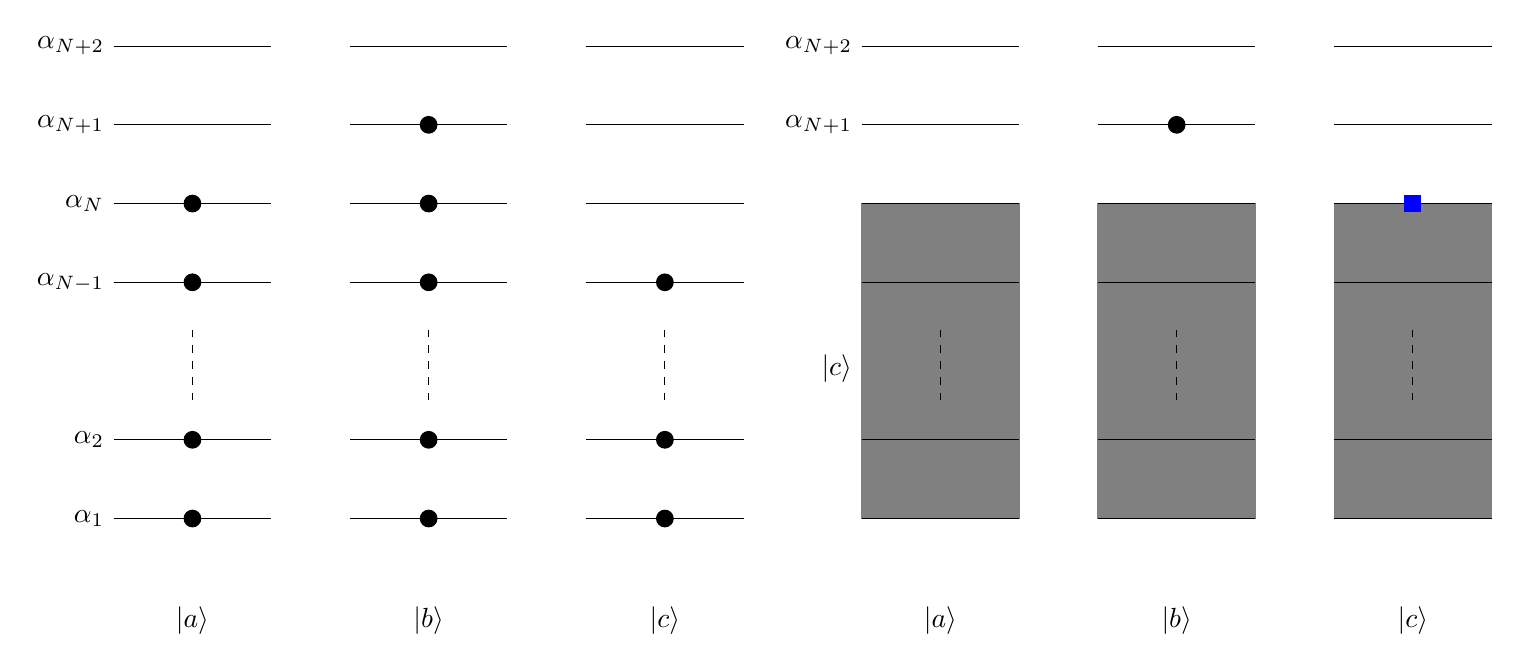
\begin{tikzpicture}
\draw (1,-1) node[anchor=north] {$\ket{a}$} -- (1,-1);
\draw (0,0) node[anchor=east] {$\alpha_1$} -- (2,0);
\draw (0,1) node[anchor=east] {$\alpha_2$} -- (2,1);
\draw (1,1.5) -- (1,1.6);
\draw (1,1.7) -- (1,1.8);
\draw (1,1.9) -- (1,2);
\draw (1,2.1) -- (1,2.2);
\draw (1,2.3) -- (1,2.4);
\draw (0,3) node[anchor=east] {$\alpha_{N-1}$} -- (2,3);
\draw (0,4) node[anchor=east] {$\alpha_N$}-- (2,4);
\draw (0,5) node[anchor=east] {$\alpha_{N+1}$}-- (2,5);
\draw (0,6) node[anchor=east] {$\alpha_{N+2}$} -- (2,6);
\filldraw [black] (1,0) circle (3pt);
\filldraw [black] (1,1) circle (3pt);
\filldraw [black] (1,3) circle (3pt);
\filldraw [black] (1,4) circle (3pt);

\draw (4,-1) node[anchor=north] {$\ket{b}$} -- (4,-1);
\draw (3,0) -- (5,0);
\draw (3,1) -- (5,1);
\draw (4,1.5) -- (4,1.6);
\draw (4,1.7) -- (4,1.8);
\draw (4,1.9) -- (4,2);
\draw (4,2.1) -- (4,2.2);
\draw (4,2.3) -- (4,2.4);
\draw (3,3) -- (5,3);
\draw (3,4) -- (5,4);
\draw (3,5) -- (5,5);
\draw (3,6) -- (5,6);
\filldraw [black] (4,0) circle (3pt);
\filldraw [black] (4,1) circle (3pt);
\filldraw [black] (4,3) circle (3pt);
\filldraw [black] (4,4) circle (3pt);
\filldraw [black] (4,5) circle (3pt);

\draw (7,-1) node[anchor=north] {$\ket{c}$} -- (7,-1);
\draw (6,0) -- (8,0);
\draw (6,1) -- (8,1);
\draw (7,1.5) -- (7,1.6);
\draw (7,1.7) -- (7,1.8);
\draw (7,1.9) -- (7,2);
\draw (7,2.1) -- (7,2.2);
\draw (7,2.3) -- (7,2.4);
\draw (6,3) -- (8,3);
\draw (6,4) -- (8,4);
\draw (6,5) -- (8,5);
\draw (6,6) -- (8,6);
\filldraw [black] (7,0) circle (3pt);
\filldraw [black] (7,1) circle (3pt);
\filldraw [black] (7,3) circle (3pt);

\draw (10.5,-1) node[anchor=north] {$\ket{a}$} -- (10.5,-1);
\filldraw [gray] (9.5,0) rectangle (11.5,4);
\draw (9.5,0) -- (11.5,0);
\draw (9.5,1) -- (11.5,1);
\draw (10.5,1.5) -- (10.5,1.6);
\draw (10.5,1.7) -- (10.5,1.8);
\draw (10.5,1.9) node[anchor=east] {$\ket{c}\hspace{1cm}$} -- (10.5,2);
\draw (10.5,2.1) -- (10.5,2.2);
\draw (10.5,2.3) -- (10.5,2.4);
\draw (9.5,3)  -- (11.5,3);
\draw (9.5,4)  -- (11.5,4);
\draw (9.5,5) node[anchor=east] {$\alpha_{{N+1}}$} -- (11.5,5);
\draw (9.5,6) node[anchor=east] {$\alpha_{N+2}$} -- (11.5,6);

\draw (13.5,-1) node[anchor=north] {$\ket{b}$} -- (13.5,-1);
\filldraw [gray] (12.5,0) rectangle (14.5,4);
\draw (12.5,0) -- (14.5,0);
\draw (12.5,1) -- (14.5,1);
\draw (13.5,1.5) -- (13.5,1.6);
\draw (13.5,1.7) -- (13.5,1.8);
\draw (13.5,1.9) -- (13.5,2);
\draw (13.5,2.1) -- (13.5,2.2);
\draw (13.5,2.3) -- (13.5,2.4);
\draw (12.5,3) -- (14.5,3);
\draw (12.5,4) -- (14.5,4);
\draw (12.5,5) -- (14.5,5);
\draw (12.5,6) -- (14.5,6);
\filldraw [black] (13.5,5) circle (3pt);

\draw (16.5,-1) node[anchor=north] {$\ket{c}$} -- (16.5,-1);
\filldraw [gray] (15.5,0) rectangle (17.5,4);
\draw (15.5,0) -- (17.5,0);
\draw (15.5,1) -- (17.5,1);
\draw (16.5,1.5) -- (16.5,1.6);
\draw (16.5,1.7) -- (16.5,1.8);
\draw (16.5,1.9) -- (16.5,2);
\draw (16.5,2.1) -- (16.5,2.2);
\draw (16.5,2.3) -- (16.5,2.4);
\draw (15.5,3) -- (17.5,3);
\draw (15.5,4) -- (17.5,4);
\draw (15.5,5) -- (17.5,5);
\draw (15.5,6) -- (17.5,6);
\filldraw [blue] (16.4, 3.9) rectangle (16.6,4.1) ;
\end{tikzpicture}}
\end{center}
\label{fig: Particle-hole figure}
\caption{Particle-Hole.}
\end{figure}

In the same way as we can construct a general slater determinant by letting the ordinary creation operators act on the vacuum state, we are now in a position to construct many-quasiparticle states by letting quasi-particle creation operators act on the reference state $\ket{r}$.
\begin{align}
\ket{ijkl..abcd..}_r \equiv \crequasi{i}\crequasi{j}\crequasi{k}\crequasi{l}..\crequasi{a}\crequasi{b}\crequasi{c}\crequasi{d}..\ket{r}.
\end{align}



\subsection{Normal-ordered Hamiltonian}

        \[
            \hat{F} = \sum_{pq} \element{p}{\hat{f}}{q} a_p^\dagger a_q
        \]
        \[
            \hat{V} = \frac{1}{4} \sum_{pqrs} \element{pq}{\hat{v}}{rs}_{AS} a_p^\dagger a_q^\dagger a_s a_r
            \equiv \frac{1}{4} \sum_{pqrs} \element{pq}{\hat{v}}{rs} a_p^\dagger a_q^\dagger a_s a_r,
        \]
        where we have defined the antisymmetric matrix elements
        \[
            \element{pq}{\hat{v}}{rs}_{AS} = \element{pq}{\hat{v}}{rs} - \element{pq}{\hat{v}}{sr}.
        \]
        \[
            \hat{V_3} = \frac{1}{36} \sum_{pqrstu} \element{pqr}{\hat{v}_3}{stu}_{AS} 
                a_p^\dagger a_q^\dagger a_r^\dagger a_u a_t a_s
            \equiv \frac{1}{36} \sum_{pqrstu} \element{pqr}{\hat{v}_3}{stu}
                a_p^\dagger a_q^\dagger a_r^\dagger a_u a_t a_s
        \]
        where we have defined the antisymmetric matrix elements
        \[
            \element{pqr}{\hat{v}_3}{stu}_{AS} = \element{pqr}{\hat{v}_3}{stu} + \element{pqr}{\hat{v}_3}{tus} + \element{pqr}{\hat{v}_3}{ust}
             - \element{pqr}{\hat{v}_3}{sut} - \element{pqr}{\hat{v}_3}{tsu} - \element{pqr}{\hat{v}_3}{uts}.
        \]
        \[
            \left\{a_a a_b \ldots a_c^\dagger a_d^\dagger\right\} = 
                (-1)^P a_c^\dagger a_d^\dagger \ldots a_a a_b
        \]
    The normal ordered Hamiltonian is given by
    \[
        \hat{H}_N = 
            \frac{1}{36} \sum_{\substack{pqr \\stu}}
                 \element{pqr}{\hat{v}_3}{stu} 
                    \normord{a^\dagger_p a^\dagger_q a^\dagger_r a_u a_t a_s}+ 
            \frac{1}{4} \sum_{pqrs} \bra{pq}\ket{rs} \normord{a^\dagger_p a^\dagger_q a_s  a_r} 
            + \sum_{pq} f_q^p \normord{a^\dagger_p a_q}= \hat{H}_3^N + \hat{V}_N + \hat{F}_N
    \]
    where
\[
        \hat{F}_N = \sum_{pq} f_q^p \normord{a^\dagger_p a_q}
\]
\[
        \hat{V}_N = \frac{1}{4} \sum_{pqrs} \bra{pq}\ket{rs} \normord{a^\dagger_p a^\dagger_q a_s  a_r} 
\]
\[
       \hat{H}_3^N = \frac{1}{36} \sum_{\substack{ pqr \\ stu}}
                     \element{pqr}{\hat{v}_3}{stu} 
                        \normord{a^\dagger_p a^\dagger_q a^\dagger_r a_u a_t a_s}
\]
    The amplitudes are given by
\[
        f_q^p = \element{p}{\hat{h}_0}{q} + \sum_i \element{pi}{\hat{v}}{qi} + \frac{1}{2} \sum_{ij} \element{pij}{\hat{v}_3}{qij}
\]
\[
        \bra{pq}{\hat{v}}\ket{rs} = \element{pq}{\hat{v}}{rs} + \sum_i \element{pqi}{\hat{v}_3}{rsi},
\]
    In relation to the Hamiltonian, $\hat{H}_N$ is given by
    \[
        \hat{H}_N = \hat{H} - E_0,
\]
\[
        E_0 = \element{\Phi_0}{\hat{H}}{\Phi_0}= \sum_i \element{i}{\hat{h}_0}{i}
                + \frac{1}{2} \sum_{ij} \element{ij}{\hat{v}}{ij}
                + \frac{1}{6} \sum_{ijk} \element{ijk}{\hat{v}_3}{ijk},
\]
    where $E_0$ is the energy expectation value between reference states.
    We start with the Hamiltonian
    \[
        \hat{H} = \hat{H}_1 + \hat{H}_2 + \hat{H}_3
    \]
    where
    \begin{subequations}
        \begin{align*}
        \hat{H}_1 &= \sum_{pq} \element{p}{\hat{h}_0}{q} a^\dagger_p a_q \\
        \hat{H}_2 &= \frac{1}{4} \sum_{pqrs} \element{pq}{\hat{v}}{rs} a^\dagger_p a^\dagger_q a_s  a_r \\
        \hat{H}_3 &= \frac{1}{36} \sum_{\substack{
                            pqr \\
                            stu}}
                     \element{pqr}{\hat{v}_3}{stu} a^\dagger_p a^\dagger_q a^\dagger_r a_u a_t a_s
        \end{align*}
    \end{subequations}
    \begin{equation*}
        \hat{H}_1 = \sum_{pq} \element{p}{\hat{h}_0}{q} a^\dagger_p a_q
    \end{equation*}

    \begin{align*}
        a^\dagger_p a_q &= \left\{a^\dagger_p a_q\right\} + \left\{ 
    \contraction{}{a}{{}^{\dagger}_p}{a}
    a^\dagger_p a_q
    \right\} \nn
        &= \left\{a^\dagger_p a_q\right\} + \delta_{pq\in i}
    \end{align*}
    \begin{align*}
        \hat{H}_1 &= \sum_{pq} \element{p}{\hat{h}_0}{q} a^\dagger_p a_q \nn
            &= \sum_{pq} \element{p}{\hat{h}_0}{q} \left\{a^\dagger_p a_q\right\} + 
                \delta_{pq\in i} \sum_{pq} \element{p}{\hat{h}_0}{q} \nn
            &= \sum_{pq} \element{p}{\hat{h}_0}{q} \left\{a^\dagger_p a_q\right\} +
                \sum_i \element{i}{\hat{h}_0}{i}
    \end{align*}
    A onebody part
    \begin{equation*}
            \hat{F}_N \Leftarrow \sum_{pq} \element{p}{\hat{h}_0}{q} \left\{a^\dagger_p a_q\right\}
    \end{equation*}
    and a scalar part
    \begin{equation*}
                E_0 \Leftarrow \sum_i \element{i}{\hat{h}_0}{i}
    \end{equation*}
    \begin{equation*}
        \hat{H}_2 = \frac{1}{4} \sum_{pqrs} \element{pq}{\hat{v}}{rs} a^\dagger_p a^\dagger_q a_s  a_r
    \end{equation*}

\begin{align*}
    a^\dagger_p a^\dagger_q a_s  a_r &= \pause
        \normord{a^\dagger_p a^\dagger_q a_s  a_r} \nn
        & \quad + \normord{
            \contraction{a^\dagger_p}{a}{{}^\dagger_q}{a}
            a^\dagger_p a^\dagger_q a_s  a_r}
        + \normord{
            \contraction{a^\dagger_p}{a}{{}^\dagger_q a_s}{a}
            a^\dagger_p a^\dagger_q a_s  a_r}
        + \normord{
            \contraction{}{a}{{}^\dagger_p a^\dagger_q}{a}
            a^\dagger_p a^\dagger_q a_s  a_r} \nn
        & \quad + \normord{
            \contraction{}{a}{{}^\dagger_p a^\dagger_q a_s}{a}
            a^\dagger_p a^\dagger_q a_s  a_r}
        + \normord{
            \contraction[1.5ex]{}{a}{{}^\dagger_p a_q^\dagger a_s}{a}
            \contraction{a^\dagger_p}{a}{{}^\dagger_q}{a}
            a^\dagger_p a^\dagger_q a_s  a_r}
        + \normord{
            \contraction{}{a}{{}^\dagger_p a_q^\dagger}{a}
            \contraction[1.5ex]{a^\dagger_p}{a}{{}^\dagger_q a_s}{a}
            a^\dagger_p a^\dagger_q a_s  a_r} \nn
    &= \normord{a^\dagger_p a^\dagger_q a_s  a_r} \nn
        & \quad + \delta_{qs\in i} \normord{ a^\dagger_p a_r}
        - \delta_{qr \in i} \normord{a^\dagger_p a_s}
        - \delta_{ps \in i} \normord{a^\dagger_q a_r} \nn
        & \quad + \delta_{pr \in i} \normord{a^\dagger_q a_s} 
        + \delta_{pr \in i} \delta_{qs \in i} - \delta_{ps \in i} \delta_{qr \in i}
\end{align*}
    \begin{align*}
    \hat{H}_2 &= \frac{1}{4} \sum_{pqrs} \element{pq}{\hat{v}}{rs} a^\dagger_p a^\dagger_q a_s  a_r \nn
        &= \frac{1}{4} \sum_{pqrs} \element{pq}{\hat{v}}{rs} \normord{a^\dagger_p a^\dagger_q a_s  a_r} 
        + \quad \frac{1}{4} \sum_{pqrs} \Bigl( 
            \delta_{qs\in i} \element{pq}{\hat{v}}{rs} \normord{ a^\dagger_p a_r} \nn
        & \quad - \delta_{qr \in i} \element{pq}{\hat{v}}{rs} \normord{a^\dagger_p a_s}
            - \delta_{ps \in i}\element{pq}{\hat{v}}{rs} \normord{a^\dagger_q a_r} \nn
        & \quad + \delta_{pr \in i} \element{pq}{\hat{v}}{rs} \normord{a^\dagger_q a_s}
            + \delta_{pr \in i} \delta_{qs \in i}
            - \delta_{ps \in i} \delta_{qr \in i} \Bigr) \nn
    \end{align*}
    \begin{align*}
        &= \frac{1}{4} \sum_{pqrs} \element{pq}{\hat{v}}{rs} \normord{a^\dagger_p a^\dagger_q a_s  a_r} \nn
        & \quad + \frac{1}{4} \sum_{pqi} \Bigl(
            \element{pi}{\hat{v}}{qi} - \element{pi}{\hat{v}}{iq} - \element{ip}{\hat{v}}{qi} + \element{ip}{\hat{v}}{iq}
        \Bigr) \normord{a^\dagger_p a_q} \nn
        & \quad + \frac{1}{4} \sum_{ij} \Bigl( 
            \element{ij}{\hat{v}}{ij}
            - \element{ij}{\hat{v}}{ji}
        \Bigr) \nn
        &= \frac{1}{4} \sum_{pqrs} \element{pq}{\hat{v}}{rs} \normord{a^\dagger_p a^\dagger_q a_s  a_r}
            + \sum_{pqi} \element{pi}{\hat{v}}{qi} \normord{a^\dagger_p a_q} 
            + \frac{1}{2} \sum_{ij} \element{ij}{\hat{v}}{ij}
    \end{align*}

\section{Stability and interpretation of the Hartree-Fock equations}
HF theory is an algorithm for a finding an approximative expression for the ground state of a given
Hamiltonian. The basic ingredients are
\begin{itemize}
\item Define a single-particle basis $\{\psi_{\alpha}\}$ so that
\[ \hat{h}^{\mathrm{HF}}\psi_{\alpha} = \varepsilon_{\alpha}\psi_{\alpha}\]
with \[\hat{h}^{\mathrm{HF}}=\hat{t}+\hat{u}_{\matrhm{ext}}+\hat{u}^{\mathrm{HF}}\]
\item where $\hat{u}^{\mathrm{HF}}$ is a single-particle potential to be determined by the HF algorithm.
\item The HF algorithm means to choose $\hat{u}^{\mathrm{HF}}$ in order to have 
\[ \langle \hat{H} \rangle = E^{\mathrm{HF}}= \langle \Phi_0 | \hat{H}|\Phi_0 \rangle\]
a local minimum with $\Phi_0$ being the SD ansatz for the ground state. 
\item The variational principle ensures that $E^{\mathrm{HF}} \ge \tilde{E}_0$, $\tilde{E}_0$ the exact ground state energy.
\end{itemize}

\subsection{Understanding the Hartree-Fock equations}


\[
|\Phi_0\rangle = \left(\prod_{i=1}^n}\hat{a}_{i}^{\dagger}\right)|0\rangle,
\]
where the $i$ define different single-particle states up to the Fermi level. We have assumed that we have $n$ fermions. 
A given one-particle-one-hole ($1p1h$) state can be written as
\[
|\Phi_i^a\rangle = \hat{a}_{a}^{\dagger}\hat{a}_i|\Phi_0\rangle,
\]
while a $2p2h$ state can be written as
\[
|\Phi_{ij}^{ab}\rangle = \hat{a}_{a}^{\dagger}\hat{a}_{b}^{\dagger}\hat{a}_j\hat{a}_i|\Phi_0\rangle,
\]
and a general $npnh$ state as 
\[
|\Phi_{ijk\dots}^{abc\dots}\rangle = \hat{a}_{a}^{\dagger}\hat{a}_{b}^{\dagger}\hat{a}_{c}^{\dagger}\dots\hat{a}_k\hat{a}_j\hat{a}_i|\Phi_0\rangle.
\]


We can then expand our exact state function for the ground state 
as
\[
|\Psi_0\rangle=C_0|\Phi_0\rangle+\sum_{ai}C_i^a|\Phi_i^a\rangle+\sum_{abij}C_{ij}^{ab}|\Phi_{ij}^{ab}\rangle+\dots
=(C_0+\hat{C})|\Phi_0\rangle,
\]
where we have introduced the so-called correlation operator 
\[
\hat{C}=\sum_{ai}C_i^a\hat{a}_{a}^{\dagger}\hat{a}_i  +\sum_{abij}C_{ij}^{ab}\hat{a}_{a}^{\dagger}\hat{a}_{b}^{\dagger}\hat{a}_j\hat{a}_i+\dots
\]
Since the normalization of $\Psi_0$ is at our disposal and since $C_0$ is by hypothesis non-zero, we may arbitrarily set $C_0=1$ with 
corresponding proportional changes in all other coefficients. Using this so-called intermediate normalization we have
\[
\langle \Psi_0 | \Phi_0 \rangle = \langle \Phi_0 | \Phi_0 \rangle = 1, 
\]
resulting in 
\[
|\Psi_0\rangle=(1+\hat{C})|\Phi_0\rangle.

We rewrite 
\[
|\Psi_0\rangle=C_0|\Phi_0\rangle+\sum_{ai}C_i^a|\Phi_i^a\rangle+\sum_{abij}C_{ij}^{ab}|\Phi_{ij}^{ab}\rangle+\dots,
\]
in a more compact form as 
\[
|\Psi_0\rangle=\sum_{PH}C_H^P\Phi_H^P=\left(\sum_{PH}C_H^P\hat{A}_H^P\right)|\Phi_0\rangle,
\]
where $H$ stands for $0,1,\dots,n$ hole states and $P$ for $0,1,\dots,n$ particle states. 
Our requirement of unit normalization gives
\[
\langle \Psi_0 | \Phi_0 \rangle = \sum_{PH}|C_H^P|^2= 1,
\]
and the energy can be written as 
\[
E= \langle \Psi_0 | \hat{H} |\Phi_0 \rangle= \sum_{PP'HH'}C_H^{*P}\langle \Phi_H^P | \hat{H} |\Phi_{H'}^{P'} \rangle C_{H'}^{P'}.
\]

Normally 
\[
E= \langle \Psi_0 | \hat{H} |\Phi_0 \rangle= \sum_{PP'HH'}C_H^{*P}\langle \Phi_H^P | \hat{H} |\Phi_{H'}^{P'} \rangle C_{H'}^{P'},
\]
is solved by diagonalization setting up the Hamiltonian matrix defined by the basis of all possible Slater determinants. A diagonalization
is equivalent to finding the variational minimum  of 
\[
 \langle \Psi_0 | \hat{H} |\Phi_0 \rangle-\lambda \langle \Psi_0 |\Phi_0 \rangle,
\]
where $\lambda$ is a variational multiplier to be identified with the energy of the system.
The minimization process results in 
\[
\delta\left[ \langle \Psi_0 | \hat{H} |\Phi_0 \rangle-\lambda \langle \Psi_0 |\Phi_0 \rangle\right]=
\sum_{P'H'}\left\{\delta[C_H^{*P}]\langle \Phi_H^P | \hat{H} |\Phi_{H'}^{P'} \rangle C_{H'}^{P'}+
C_H^{*P}\langle \Phi_H^P | \hat{H} |\Phi_{H'}^{P'} \rangle \delta[C_{H'}^{P'}]  .\right
\]
\[
.\left -
\lambda( \delta[C_H^{*P}]C_{H'}^{P'}+C_H^{*P}\delta[C_{H'}^{P'}]\right\} = 0.
\]
Since the coefficients $\delta[C_H^{*P}]$ and $\delta[C_{H'}^{P'}]$ are complex conjugates it is necessary and sufficient to require the quantities that multiply with $\delta[C_H^{*P}]$ to vanish.  


An alternative way to derive the last equation is to start from 
\[
(\hat{H} -E)|\Psi_0\rangle = (\hat{H} -E)\sum_{P'H'}C_{H'}^{P'}|\Phi_{H'}^{P'} \rangle=0, 
\]
and if this equation is successively projected against all $\Phi_H^P$ in the expansion of $\Psi$, then the last equation on the previous slide
results.   As stated previously, one solves this equation normally by diagonalization. If we are able to solve this equation exactly (that is
numerically exactly) in a large Hilbert space (it will be truncated in terms of the number of single-particle states included in the definition
of Slater determinants), it can then serve as a benchmark for other many-body methods which approximate the correlation operator
$\hat{C}$.  

For reasons to come (link with Coupled-Cluster theory and Many-Body perturbation theory), 
we will rewrite Eq.~(\ref{eq:fullci}) as a set of coupled non-linear equations in terms of the unknown coefficients $C_H^P$. 


To see this, we look at $ \langle \Phi_H^P | = \langle \Phi_0 |$ in  Eq.~(\ref{eq:fullci}), that is we multiply with $\langle \Phi_0 |$
from the left in 
\[
(\hat{H} -E)\sum_{P'H'}C_{H'}^{P'}|\Phi_{H'}^{P'} \rangle=0, 
\]
and we assume that we have a two-body operator at most.  Using Slater's rule gives then and equation for the 
correlation energy in terms of $C_i^a$ and $C_{ij}^{ab}$.  We get then
\[
\langle \Phi_0 | \hat{H} -E| \Phi_0\rangle + \sum_{ai}\langle \Phi_0 | \hat{H} -E|\Phi_{i}^{a} \rangle C_{i}^{a}+
\sum_{abij}\langle \Phi_0 | \hat{H} -E|\Phi_{ij}^{ab} \rangle C_{ij}^{ab}=0,
\]
or 
\[
E-E_0 =\Delta E=\sum_{ai}\langle \Phi_0 | \hat{H}|\Phi_{i}^{a} \rangle C_{i}^{a}+
\sum_{abij}\langle \Phi_0 | \hat{H}|\Phi_{ij}^{ab} \rangle C_{ij}^{ab},
\]
where the $E_0$ is the reference energy and $\Delta E$ becomes the correlation energy.
We have already computed the expectation values $\langle \Phi_0 | \hat{H}|\Phi_{i}^{a} $ and $\langle \Phi_0 | \hat{H}|\Phi_{ij}^{ab}\rangle$.

We can rewrite
\[
E-E_0 =\Delta E=\sum_{ai}\langle \Phi_0 | \hat{H}|\Phi_{i}^{a} \rangle C_{i}^{a}+
\sum_{abij}\langle \Phi_0 | \hat{H}|\Phi_{ij}^{ab} \rangle C_{ij}^{ab},
\]
as
\[
\Delta E=\sum_{ai}\langle i| \hat{f}|a \rangle C_{i}^{a}+
\sum_{abij}\langle ij | \hat{v}| ab \rangle C_{ij}^{ab}.
\]
This equation determines the correlation energy but not the coefficients $C$. 
We need more equations. Our next step is to set up
\[
\langle \Phi_i^a | \hat{H} -E| \Phi_0\rangle + \sum_{bj}\langle \Phi_i^a | \hat{H} -E|\Phi_{j}^{b} \rangle C_{j}^{b}+
\sum_{bcjk}\langle \Phi_i^a | \hat{H} -E|\Phi_{jk}^{bc} \rangle C_{jk}^{bc}+
\sum_{bcdjkl}\langle \Phi_i^a | \hat{H} -E|\Phi_{jkl}^{bcd} \rangle C_{jkl}^{bcd}=0,
\]
as this equation will allow us to find an expression for the coefficents $C_i^a$ since we can rewrite this equation as 
\[
\langle i | \hat{f}| a\rangle +\langle \Phi_i^a | \hat{H}|\Phi_{i}^{a} \rangle C_{i}^{a}+ \sum_{bj\ne ai}\langle \Phi_i^a | \hat{H}|\Phi_{j}^{b} \rangle C_{j}^{b}+
\sum_{bcjk}\langle \Phi_i^a | \hat{H}|\Phi_{jk}^{bc} \rangle C_{jk}^{bc}+
\sum_{bcdjkl}\langle \Phi_i^a | \hat{H}|\Phi_{jkl}^{bcd} \rangle C_{jkl}^{bcd}=0.
\]


Let us now compute the Hamiltonian matrix for a system consisting of a
Slater determinant for the ground state $|\Phi_0 \rangle$ and two 1p1h
SDs $|\Phi_i^a \rangle$ and $|\Phi_j^b \rangle$. This can obviously be
generalized to many more 1p1h SDs.  We will show later that we get the
following expectation values
\[ \langle \Phi_0 | \hat{H}|\Phi_0 \rangle = E_0, \]
\[ \langle \Phi_i^a | \hat{H}|\Phi_0 \rangle = \langle a | \hat{f} | i \rangle,\]
\[ \langle \Phi_j^b | \hat{H}|\Phi_0 \rangle = \langle b | \hat{f} | j \rangle,\]
\[\langle \Phi_i^a | \hat{H}|\Phi_j^b \rangle = \langle aj | \hat{v} | ib \rangle,\]
and the diagonal elements
\[ \langle \Phi_i^a | \hat{H}|\Phi_i^a \rangle = E_0+\varepsilon_{a}-\varepsilon_{i}+\langle ai | \hat{v} | ia \rangle,\]
and
\[ \langle \Phi_j^b | \hat{H}|\Phi_j^b \rangle =E_0+\varepsilon_{b}-\varepsilon_{j}+\langle bj | \hat{v} | jb \rangle.\]

We can then set up a Hamiltonian matrix to be diagonalized
\[
 \left( \begin{array}{ccc} E_0 & \langle i | \hat{f} | a \rangle &
   \langle j | \hat{f} | b\rangle\\ \langle a | \hat{f} | i \rangle
   &E_0+\varepsilon_{a}-\varepsilon_{i}+\langle ai | \hat{v} | ia
   \rangle & \langle aj | \hat{v} | ib \rangle \\ \langle b | \hat{f}
   | j \rangle & \langle bi | \hat{v} | ja \rangle
   &E_0+\varepsilon_{b}-\varepsilon_{j}+\langle bj | \hat{v} | jb
   \rangle \\
             \end{array} \right) .
\]
The HF method corresponds to finding a similarity transformation where
the non-diagonal matrix elements
\[\langle i | \hat{f} | a \rangle=0\].   We will link this expectation value with the HF method, meaning that
we want to find
\[\langle i | \hat{h}^{\mathrm{HF}}| a \rangle=0\]


\subsection{Stability of Hartree-Fock equations}


Last week we computed the Hamiltonian matrix for a system consisting of a Slater determinant for the ground state 
$|\Phi_0 \rangle$ and two 1p1h SDs $|\Phi_i^a \rangle$ and $|\Phi_j^b \rangle$. This can obviously be generalized to many more 1p1h SDs.  Using diagrammatic as well as algebraic representations we found the following 
expectation values
\[ \langle \Phi_0 | \hat{H}|\Phi_0 \rangle = E_0, \]
\[ \langle \Phi_i^a | \hat{H}|\Phi_0 \rangle = \langle a | \hat{f} | i \rangle,\]
\[ \langle \Phi_j^b | \hat{H}|\Phi_0 \rangle = \langle b | \hat{f} | j \rangle,\]
\[\langle \Phi_i^a | \hat{H}|\Phi_j^b \rangle = \langle aj | \hat{v} | ib \rangle,\]
and the diagonal elements
\[ \langle \Phi_i^a | \hat{H}|\Phi_i^a \rangle = E_0+\varepsilon_{a}-\varepsilon_{i}+\langle ai | \hat{v} | ia \rangle,\]
and 
\[ \langle \Phi_j^b | \hat{H}|\Phi_j^b \rangle =E_0+\varepsilon_{b}-\varepsilon_{j}+\langle bj | \hat{v} | jb \rangle.\]
We can then set up a Hamiltonian matrix to be diagonalized
\[
 \left( \begin{array}{ccc} 
               E_0  & \langle i | \hat{f} | a \rangle &  \langle j | \hat{f} | b\rangle\\
               \langle a | \hat{f} | i \rangle  &E_0+\varepsilon_{a}-\varepsilon_{i}+\langle ai | \hat{v} | ia \rangle  & \langle aj | \hat{v} | ib \rangle      \\
               \langle b | \hat{f} | j \rangle  & \langle bi | \hat{v} | ja \rangle &E_0+\varepsilon_{b}-\varepsilon_{j}+\langle bj | \hat{v} | jb \rangle         \\
             \end{array} \right) .
\]
The HF method corresponds to finding a similarity transformation where the non-diagonal matrix elements
\[\langle i | \hat{f} | a \rangle=0\].   We will link this expectation value with the HF method, meaning that
we want to find
\[\langle i | \hat{h}^{\mathrm{HF}}| a \rangle=0\]
We wish now to derive the Hartree-Fock equations using our second-quantized formalism and study the stability of the equations. 
Our SD ansatz for the ground state of the system is approximated as
\[   |\Phi_0\rangle = |c\rangle = \cre{i} \cre{j}\dots\cre{l}|0\rangle.\]
We wish to determine $\hat{u}^{HF}$ so that 
$E_0^{HF}= \langle c|\hat{H}| c\rangle$ becomes a local minimum. 


An arbitrary Slater determinant $\ket{c'}$ which is not orthogonal to a determinant
$\ket{c}={\displaystyle\prod_{i=1}^{n}}
a_{\alpha_{i}}^{\dagger}\ket{0}$, can be written as
\[
\ket{c'}=exp\left\{\sum_{a>F}\sum_{i\le F}C_{ai}a_{a}^{\dagger}
a_{i}\right\}\ket{c}
\]

The variational condition for deriving the Hartree-Fock equations guarantees only that the expectation value
$\langle c | \hat{H} | c \rangle$ has an extreme value, not necessarily a minimum. To figure out whether the extreme value we have found  is a minimum, we can use second quantization to analyze our results and find a criterion 
for the above expectation value to a local minimum. We will use Thouless' theorem and show that
\[
\frac{\langle c' |\hat{H} | c'\rangle}{\langle c' |c'\rangle} \ge \langle c |\hat{H} | c\rangle= E_0,
\]
with 
\[
|c'\rangle = |c\rangle + |\delta c\rangle.
\]
Using Thouless' theorem we can write out $|c'\rangle$ as
\[
\ket{c'}=exp\left\{\sum_{a>F}
\sum_{i\le F}\delta C_{ai}a_{a}^{\dagger}
a_{i}\right\}\ket{c}=
\]
\[
\left\{1+\sum_{a>F}\sum_{i\le F}\delta C_{ai}a_{a}^{\dagger}
a_{i}+\frac{1}{2!}\sum_{ab>F}
\sum_{ij\le F}\delta C_{ai}\delta C_{bj}a_{a}^{\dagger}a_{i}a_{b}^{\dagger}a_{j}+\dots\right\}
\]
where the amplitudes $\delta C$ are small.

The norm of $|c'\rangle$ is given by (using the intermediate normalization condition $\langle c' |c\rangle=1$) 
\[
\langle c' | c'\rangle = 1+\sum_{a>F}
\sum_{i\le F}|\delta C_{ai}|^2+O(\delta C_{ai}^3).
\]
The expectation value for the energy is now given by (using the Hartree-Fock condition)
\[
\langle c' |\hat{H} | c'\rangle=\langle c |\hat{H} | c\rangle +
\sum_{ab>F}
\sum_{ij\le F}\delta C_{ai}^*\delta C_{bj}\langle c |a_{i}^{\dagger}a_{a}\hat{H}a_{b}^{\dagger}a_{j}|c\rangle+
\]
\[
\frac{1}{2!}\sum_{ab>F}
\sum_{ij\le F}\delta C_{ai}\delta C_{bj}\langle c |\hat{H}a_{a}^{\dagger}a_{i}a_{b}^{\dagger}a_{j}|c\rangle+\frac{1}{2!}\sum_{ab>F}
\sum_{ij\le F}\delta C_{ai}^*\delta C_{bj}^*\langle c|a_{j}^{\dagger}a_{b}a_{i}^{\dagger}a_{a}\hat{H}|c\rangle
+\dots
\] 
We will skip higher-order terms later.

We have already calculated the second term on the rhs of the previous equation
\[
\bra{c} \left(\normord{a^\dagger_i a_a} \op{H} \normord{a^\dagger_b a_j} \right) \ket{c} =
\]
\[
\sum_{pq} \sum_{ijab}\delta C_{ai}^*\delta C_{bj} \bra{p}\hat{h}_0\ket{q} 
            \bra{c} \left(\normord{a^\dagger_i a_a}\normord{a^\dagger_pa_q} 
             \normord{a^\dagger_b a_j} \right)\ket{c}+ 
\]
\[
\frac{1}{4} \sum_{pqrs} \sum_{ijab}\delta C_{ai}^*\delta C_{bj} \bra{pq}\hat{v}\ket{rs} 
            \bra{c} \left(\normord{a^\dagger_i a_a}\normord{a^\dagger_p a^\dagger_q a_s  a_r} \normord{a^\dagger_b a_j} \right)\ket{c},
\]
resulting in
\[
E_0\sum_{ai}|\delta C_{ai}|^2+\sum_{ai}|\delta C_{ai}|^2(\varepsilon_a-\varepsilon_i)-\sum_{ijab} \bra{aj}\hat{v}\ket{bi}\delta C_{ai}^*\delta C_{bj}.
\]

The third term in the rhs of the last equation can then be written out (where is the reference energy and why do we only consider the two-particle interaction $\hat{V}_N$?)
    \begin{align*}
        & \frac{1}{2!}\bra{c}  \left( \op{V}_N \normord{a^\dagger_a a_i} \normord{a^\dagger_b a_j} \right) \ket{c} = \\
            & \quad \frac{1}{8} \sum_{pqrs} \sum_{ijab}\delta C_{ai}\delta C_{bj} \bra{pq}\hat{v}\ket{rs} 
            \bra{c} \left(\normord{a^\dagger_p a^\dagger_q a_s  a_r} 
            \normord{a^\dagger_a a_i} \normord{a^\dagger_b a_j} \right)\ket{c} \\
        &= \frac{1}{8} \sum_{pqrs} \sum_{ijab} \bra{pq}\hat{v}\ket{rs} \delta C_{ai}\delta C_{bj} \bra{c} \\
        & \quad \Bigl( 
        \left\{
        \contraction{a^\dagger_p a^\dagger_q a_s}{a}{{}_r}{a}
        \contraction[1.25ex]{a^\dagger_p}{a}{{}^\dagger_q a_s a_r a^\dagger_a}{a}
        \contraction[1.5ex]{a^\dagger_p a^\dagger_q }{a}{{}_s a_r a^\dagger_a a_i}{a}
        \contraction[1.75ex]{}{a}{{}^\dagger_p a^\dagger_q a_s a_r a^\dagger_a a_i a^\dagger_b}{a}
        a^\dagger_p a^\dagger_q a_s  a_r a^\dagger_a a_i a^\dagger_b a_j \right\}
        +\left\{
        \contraction{a^\dagger_p a^\dagger_q}{a}{{}_s a_r}{a}
        \contraction[1.25ex]{a^\dagger_p}{a}{{}^\dagger_q a_s a_r a^\dagger_a}{a}
        \contraction[1.5ex]{a^\dagger_p a^\dagger_q a_s}{a}{{}_r a^\dagger_a a_i}{a}
        \contraction[1.75ex]{}{a}{{}^\dagger_p a^\dagger_q a_s a_r a^\dagger_a a_i a^\dagger_b}{a}
        a^\dagger_p a^\dagger_q a_s  a_r a^\dagger_a a_i a^\dagger_b a_j \right\}
        + \left\{
        \contraction{a^\dagger_p a^\dagger_q a_s}{a}{{}_r}{a}
        \contraction[1.25ex]{}{a}{{}^\dagger_p q^\dagger_q a_s a_r a^\dagger_a}{a}
        \contraction[1.5ex]{a^\dagger_p a^\dagger_q }{a}{{}_s a_r a^\dagger_a a_i}{a}
        \contraction[1.75ex]{a^\dagger_p}{a}{{}^\dagger_q a_s a_r a^\dagger_a a_i a^\dagger_b}{a}
        a^\dagger_p a^\dagger_q a_s  a_r a^\dagger_a a_i a^\dagger_b a_j \right\} \\
        & \quad +\left\{
        \contraction{a^\dagger_p a^\dagger_q}{a}{{}_s a_r}{a}
        \contraction[1.25ex]{}{a}{{}^\dagger_p q^\dagger_q a_s a_r a^\dagger_a}{a}
        \contraction[1.5ex]{a^\dagger_p a^\dagger_q a_s}{a}{{}_r a^\dagger_a a_i}{a}
        \contraction[1.75ex]{a^\dagger_p}{a}{{}^\dagger_q a_s a_r a^\dagger_a a_i a^\dagger_b}{a}
        a^\dagger_p a^\dagger_q a_s  a_r a^\dagger_a a_i a^\dagger_b a_j \right\}
        \Bigr) \ket{c} \\
        &= \frac{1}{2} \sum_{ijab} \bra{ij}\hat{v}\ket{ab}\delta C_{ai}\delta C_{bj}
    \end{align*}
The final term in the rhs of the last equation can then be written out as
    \[
\frac{1}{2!}\bra{c}\left(\normord{a^\dagger_j a_b} \normord{a^\dagger_i a_a} \op{V}_N  \right) \ket{c} = 
\frac{1}{2!}\bra{c}\left( \op{V}_N \normord{a^\dagger_a a_i} \normord{a^\dagger_b a_j} \right)^{\dagger} \ket{c}
\]
which is nothing but
\[
\frac{1}{2!}\bra{c}  \left( \op{V}_N \normord{a^\dagger_a a_i} \normord{a^\dagger_b a_j} \right) \ket{c}^*
=\frac{1}{2} \sum_{ijab} (\bra{ij}\hat{v}\ket{ab})^*\delta C_{ai}^*\delta C_{bj}^*
\]
or 
\[
\frac{1}{2} \sum_{ijab} (\bra{ab}\hat{v}\ket{ij})\delta C_{ai}^*\delta C_{bj}^*
\]
where we have used the relation
\[ \langle a |\hat{A} | b\rangle =  (\langle b |\hat{A}^{\dagger} | a\rangle)^*
\]
due to the hermiticity of $\hat{H}$ and $\hat{V}$.
We define two matrix elements
\[
A_{ai,bj}=-\bra{aj}\hat{v}\ket{bi}
\]
\[
B_{ai,bj}=\bra{ab}\hat{v}\ket{ij}
\]
both being anti-symmetrized.
We can then write out the energy
\[
\langle c'|H|c'\rangle = \left(1+\sum_{ai}|\delta C_{ai}|^2\right)\langle c |H|c\rangle+
\]
\[
\sum_{ai}|\delta C_{ai}|^2(\varepsilon_a^{HF}-\varepsilon_i^{HF})+\sum_{ijab}A_{ai,bj}\delta C_{ai}^*\delta C_{bj}+
\]
\[
\frac{1}{2} \sum_{ijab} B_{ai,bj}^*\delta C_{ai}\delta C_{bj}+\frac{1}{2} \sum_{ijab} B_{ai,bj}\delta C_{ai}^*\delta C_{bj}^*
+O(\delta C_{ai}^3),\]
which allows us to rewrite it as 
\[
\langle c'|H|c'\rangle = \left(1+\sum_{ai}|\delta C_{ai}|^2\right)\langle c |H|c\rangle+\Delta E+O(\delta C_{ai}^3),
\]
and skipping higher-order terms we have
\[
\frac{\langle c' |\hat{H} | c'\rangle}{\langle c' |c'\rangle} =E_0+\frac{\Delta E}{\left(1+\sum_{ai}|\delta C_{ai}|^2\right)}.
\]

We have defined 
\[
\Delta E = \frac{1}{2} \langle \chi | \hat{M}| \chi \rangle
\]
with the vectors 
\[ \chi = \left[ \delta C\hspace{0.2cm} \delta C^*\right]^T
\]
and the matrix 
\[
\hat{M}=\left(\begin{array}{cc} \Delta + A & B \\ B^* & \Delta + A^*\end{array}\right),
\]
with $\Delta_{ai,bj} = (\varepsilon_a-\varepsilon_i)\delta_{ab}\delta_{ij}$.
The condition
\[
\Delta E = \frac{1}{2} \langle \chi | \hat{M}| \chi \rangle \ge 0
\]
for an arbitrary  vector 
\[ \chi = \left[ \delta C\hspace{0.2cm} \delta C^*\right]^T\]
means that all eigenvalues of the matrix have to be larger than or equal zero. 
A necessary (but no sufficient) condition is that the matrix elements (for all $ai$ )
\[
(\varepsilon_a-\varepsilon_i)\delta_{ab}\delta_{ij}+A_{ai,bj} \ge 0.
\]
This equation can be used as a first test of the stability of the Hartree-Fock equation.




\section{Diagrams}
Although Wick's theorem adds considerable simplifications to the calculation of various expectation values, the human brain is, sadly, not well suited for finding complicated combinations of
contractions using Wick's theorem.
As an example, we present a string of operators
arising from the evaluation of the transition probability from a 1p-1h excitation
to another 1p-1h excitation for the two-body potential, 
\begin{equation}
\label{eq:manybody:example}
\langle \Phi_i^a | \hat{V} | \Phi_j^b \rangle
\rightarrow
\hat{i}^{\dagger} \hat{a} \hspace{2mm} \hat{p}^{\dagger} \hat{q}^{\dagger}
\hat{s} \hat{r} \hspace{2mm} \hat{b}^{\dagger} \hat{j} .
\end{equation}
Although this expression only contains eight operators, it leads to fourteen nonzero,
fully contracted, terms.
One needs to be focused and systematic in order to calculate all terms correctly.
However, the brain seems to be good at visualizing mental images, and therefore a
graphical presentation of the formulas could serve us well.


The graphical approach presented here originated in quantum field theory,
developed by Richard Feynman~\cite{RevModPhys.20.367,PhysRev.76.769}.
Although originally meant to be used on time dependent transitions from one
state to another, it is presented here without a time ordering (following~\cite{shavitt2009many}).
It does, however, restrict the order in which operators are applied.

Diagrams start out with the reference ket state, denoted by two horizontal lines at
the bottom, and end out with the reference bra state, as two horizontal lines
at the top. 
Particle operators are lines pointing upwards, whereas holes point downwards.
In this fashion, determinants with excitations from the reference state can be visualized as
\begin{eqnarray}
\langle \Phi_i^a | = \langle \Phi | \hat{i}^{\dagger}\hat{a} =& 
\parbox{30mm}{
    \textrm{
    \begin{fmffile}{fmf-oneponehbra}
        \begin{fmfgraph*}(50,50)
            \fmfbottom{i1,i2} \fmftop{o1,o2}
            \fmf{phantom}{i1,hb,pb,i2}
            \fmf{double}{o1,ht,pt,o2}
            \fmffreeze
            \fmf{electron,label=$i$}{ht,hb}
            \fmf{electron,label=$a$}{pb,pt}
        \end{fmfgraph*}
    \end{fmffile}
    }
} \\
|\Phi_{ij}^{ab} \rangle = \hat{a}^{\dagger}\hat{b}^{\dagger}\hat{j}\hat{i}|\Phi \rangle =& 
\parbox{40mm}{
    \textrm{
    \begin{fmffile}{fmf-twoptwohket}
        \begin{fmfgraph*}(100,50)
            \fmfbottom{i1,i2} \fmftop{o1,o2}
            \fmf{double}{i1,h1b,p1b,dummyb,h2b,p2b,i2}
            \fmf{phantom}{o1,h1t,p1t,dummyt,h2t,p2t,o2}
            \fmffreeze
            \fmf{electron,label=$i$}{h1t,h1b}
            \fmf{electron,label=$a$}{p1b,p1t}
            \fmf{electron,label=$j$}{h2t,h2b}
            \fmf{electron,label=$b$}{p2b,p2t}
        \end{fmfgraph*}
    \end{fmffile}
    }
} .
\end{eqnarray}


One-body operators are presented as two electron lines connected to a dashed line with a cross,
\begin{equation}
\hat{H^{(0)}} = \sum_{pq} \langle p | \hat{h^{(0)}} | \hat{q} \rangle \hat{p}^{\dagger}\hat{q} =
\parbox{30mm}{
	\textrm{
	\begin{fmffile}{fmf-onebodyoperator}
		\begin{fmfgraph*}(50,50)
			\fmfbottom{i1,i2} \fmftop{o1,o2}
			\fmf{electron,label=$q$}{i1,f1}
			\fmf{electron,label=$p$}{f1,o1}
			\fmf{dashes}{f1,f2}
			\fmfv{decor.shape=cross}{f2}
			\fmf{phantom}{i2,f2}
			\fmf{phantom}{f2,o2}
		\end{fmfgraph*}
	\end{fmffile}
	}
}
\end{equation}
Two-body operators are represented similarly, but have two incoming and two outgoing lines due to the two-body nature,
\begin{equation}
\hat{H}^{(1)} = \frac{1}{4}\sum_{pqrs} \langle pq | | rs \rangle \hat{p}^{\dagger}\hat{q}^{\dagger} \hat{s} \hat{r} =
\parbox{30mm}{
	\textrm{
	\begin{fmffile}{fmf-twobodyoperator}
		\begin{fmfgraph*}(50,50)
			\fmfbottom{i1,i2} \fmftop{o1,o2}
			\fmf{electron,label=$r$}{i1,f1}
			\fmf{electron,label=$p$}{f1,o1}
			\fmf{dashes}{f1,f2}
			\fmf{electron,label=$s$}{i2,f2}
			\fmf{electron,label=$q$}{f2,o2}
		\end{fmfgraph*}
	\end{fmffile}
	}
} .
\end{equation}


The idea now is to represent contractions by connecting lines, and because only fully contracted terms are nonzero within the reference state, all lines should be connected.
All \textit{free} indexes are meant to be summed over, and the matrix elements are found by replacing $q$ with the label of incoming line and $p$ with the outgoing label in the one-body case.
In the two-body case we replace $r/s$ with left/right incoming line and $p/q$ with left/right outgoing line.
To determine the correct phase factor, one needs to count the number of hole lines and the number of closed paths.
When counting the number of closed paths we will consider associated particle-hole pairs as if they were connected in the reference states.
The phase factor will in the end be $(-1)^{l + h}$, where $l$ is the number of closed paths (loops) and $h$ is the number of hole lines.


To illustrate the use of diagrams, we return to the example in the introduction, eq.~\eqref{eq:manybody:example}.
This expression is evaluated to four unique ways of connecting the diagrams;

\begin{equation}
\label{eq:manybody:iavbjDiag}
\begin{split}
\langle \Phi_i^a | \hat{V} | \Phi_j^b \rangle
&= 
\overbrace{
\parbox{35mm}{
	\textrm{
	\begin{fmffile}{fmf-example-term1}
		\begin{fmfgraph*}(80,80) \fmfkeep{fmf-example-term1}
			\fmfbottom{i1,i2} \fmftop{o1,o2}
			%Reference states
			\fmf{double}{i1,b1,dummy1,b2,i2}
			\fmf{double}{o1,t1,dummy2,t2,o2}
			\fmffreeze
			%Operator line
			\fmf{dashes}{g1,g2}
			%Electrons		
			\fmf{electron,label=$j$}{g1,b1}
			\fmf{electron,label=$b$}{b2,g2}
			\fmf{electron,label=$i$}{t1,g1}
			\fmf{electron,label=$a$}{g2,t2}
		\end{fmfgraph*}
	\end{fmffile}
	}
}
}^{(a)}
+
\overbrace{
\parbox{35mm}{
	\textrm{
	\begin{fmffile}{fmf-example-term2}
		\begin{fmfgraph*}(80,80) \fmfkeep{fmf-example-term2}
			\fmfbottom{i1,i2} \fmftop{o1,o2}
			%Reference states
			\fmf{double}{i1,b1,dummy1,b2,i2}
			\fmf{double}{o1,t1,dummy2,t2,o2}
			\fmffreeze
			%Operator line
			\fmf{dashes}{g1,g2}
			\fmf{phantom}{b1,loop}
			\fmf{phantom}{t1,loop}
			%Electrons		
			\fmf{electron,label=$b$}{b2,g2}
			\fmf{electron,label=$a$}{g2,t2}
			\fmf{electron,label=$i$}{t1,holeconnect}
			\fmf{electron,label=$j$}{holeconnect,b1}
			%Electron hole loop
			\fmf{electron,right,tension=0.3,label=$k$}{g1,loop}
			\fmf{electron,right,tension=0.3}{loop,g1}
		\end{fmfgraph*}
	\end{fmffile}
	}
}
}^{(b)} \\
&+
\underbrace{
\parbox{35mm}{
	\textrm{
	\begin{fmffile}{fmf-example-term3}
		\begin{fmfgraph*}(80,80) \fmfkeep{fmf-example-term3}
			\fmfbottom{i1,i2} \fmftop{o1,o2}
			%Reference states
			\fmf{double}{i1,b1,dummy1,b2,i2}
			\fmf{double}{o1,t1,dummy2,t2,o2}
			\fmffreeze
			%Operator line
			\fmf{dashes}{g1,g2}
			\fmf{phantom}{b2,loop}
			\fmf{phantom}{t2,loop}
			%Electrons		
			\fmf{electron,label=$b$}{b2,partconnect}
			\fmf{electron,label=$a$}{partconnect,t2}
			\fmf{electron,label=$i$}{t1,g1}
			\fmf{electron,label=$j$}{g1,b1}
			%Electron hole loop
			\fmf{electron,left,tension=0.3}{g2,loop}
			\fmf{electron,left,tension=0.3,label=$k$}{loop,g2}
		\end{fmfgraph*}
	\end{fmffile}
	}
}
}_{(c)}
+
\underbrace{
\parbox{35mm}{
	\textrm{
	\begin{fmffile}{fmf-example-term4}
		\begin{fmfgraph*}(80,80) \fmfkeep{fmf-example-term4}
			\fmfbottom{i1,i2} \fmftop{o1,o2}
			%Reference states
			\fmf{double}{i1,b1,b2,b3,b4,b5,i2}
			\fmf{double}{o1,t1,t2,t3,t4,t5,o2}
			\fmffreeze
			%Connecting points for hole loops
			\fmf{phantom}{b3,loop1,t3}
			\fmf{phantom}{i2,loop2,o2}
			\fmffreeze
			%Operator
			\fmf{dashes}{g1,g2}
			%Hole loops
			\fmf{electron,right,label=$k$,tension=0.3}{g1,loop1}
			\fmf{electron,right,tension=0.3}{loop1,g1}
			\fmf{electron,left,label=$l$,tension=0.3}{g2,loop2}
			\fmf{electron,left,tension=0.3}{loop2,g2}
			%Electronlines
			\fmf{electron,label=$i$}{t1,holeconnect}
			\fmf{electron,label=$j$}{holeconnect,b1}
			\fmf{electron,label=$b$}{b2,partconnect}
			\fmf{electron,label=$a$}{partconnect,t2}
		\end{fmfgraph*}
	\end{fmffile}
	}
} 
}_{(d)}
.
\end{split}
\end{equation}
\begin{enumerate}[{\bf Term (\ref{eq:manybody:iavbjDiag}a)}]
\item has no free indexes since all lines are connected to the particle and hole indices already defined in the reference states.
The corresponding matrix element is $\langle ja || ib \rangle$.
Having two hole lines, one closed loop, and in total four equal terms, 
\begin{equation}
\parbox{23mm}{
	\textrm{
	\begin{fmffile}{fmf-example-term1-1}
		\begin{fmfgraph*}(50,50)
			\fmfbottom{i1,i2} \fmftop{o1,o2}
			%Reference states
			\fmf{double}{i1,b1,dummy1,b2,i2}
			\fmf{double}{o1,t1,dummy2,t2,o2}
			\fmffreeze
			%Operator line
			\fmf{dashes}{g1,g2}
			%Electrons		
			\fmf{electron}{g1,b1}
			\fmf{electron}{b2,g2}
			\fmf{electron}{t1,g1}
			\fmf{electron}{g2,t2}
		\end{fmfgraph*}
	\end{fmffile}
	}
}
=
\parbox{23mm}{
	\textrm{
	\begin{fmffile}{fmf-example-term1-2}
		\begin{fmfgraph*}(50,50) \fmfkeep{fmf-example-term1-2}
			\fmfbottom{i1,i2} \fmftop{o1,o2}
			%Reference states
			\fmf{double}{i1,b1,dummy1,b2,i2}
			\fmf{double}{o1,t1,dummy2,t2,o2}
			\fmffreeze
			%Operator line
			\fmf{dashes}{g1,g2}
			\fmf{phantom}{g1,b1}
			\fmf{phantom}{b2,g2}
			\fmf{phantom}{t1,g1}
			\fmf{phantom}{g2,t2}			
			\fmffreeze
			%Electrons		
			\fmf{electron}{g2,b1}
			\fmf{electron}{b2,g1}
			\fmf{electron}{t1,g2}
			\fmf{electron}{g1,t2}
		\end{fmfgraph*}
	\end{fmffile}
	}
}
=
\parbox{23mm}{
	\textrm{
	\begin{fmffile}{fmf-example-term1-3}
		\begin{fmfgraph*}(50,50) \fmfkeep{fmf-example-term1-3}
			\fmfbottom{i1,i2} \fmftop{o1,o2}
			%Reference states
			\fmf{double}{i1,b1,dummy1,b2,i2}
			\fmf{double}{o1,t1,dummy2,t2,o2}
			\fmffreeze
			%Operator line
			\fmf{dashes}{g1,g2}
			\fmf{phantom}{g1,b1}
			\fmf{phantom}{b2,g2}
			\fmf{phantom}{t1,g1}
			\fmf{phantom}{g2,t2}			
			\fmffreeze
			%Electrons		
			\fmf{electron}{g1,b1}
			\fmf{electron}{b2,g1}
			\fmf{electron}{t1,g2}
			\fmf{electron}{g2,t2}
		\end{fmfgraph*}
	\end{fmffile}
	}
}
=
\parbox{23mm}{
	\textrm{
	\begin{fmffile}{fmf-example-term1-4}
		\begin{fmfgraph*}(50,50) \fmfkeep{fmf-example-term1-4}
			\fmfbottom{i1,i2} \fmftop{o1,o2}
			%Reference states
			\fmf{double}{i1,b1,dummy1,b2,i2}
			\fmf{double}{o1,t1,dummy2,t2,o2}
			\fmffreeze
			%Operator line
			\fmf{dashes}{g1,g2}
			\fmf{phantom}{g1,b1}
			\fmf{phantom}{b2,g2}
			\fmf{phantom}{t1,g1}
			\fmf{phantom}{g2,t2}			
			\fmffreeze
			%Electrons		
			\fmf{electron}{g2,b1}
			\fmf{electron}{b2,g2}
			\fmf{electron}{t1,g1}
			\fmf{electron}{g1,t2}
		\end{fmfgraph*}
	\end{fmffile}
	}
} ,
\end{equation}
the total factor in front should be $(-1)^{2+1} \cdot 4 \cdot \frac{1}{4} = -1$.
\item corresponds to the element $\delta_{ij} \langle ka || kb \rangle$, where the Kronecker delta function follows from the contracted hole lines between $i$ and $j$.
There are two hole lines, two loops, and in total four equal terms,
\begin{equation}
\parbox{23mm}{
	\textrm{
	\begin{fmffile}{fmf-example-term2-1}
		\begin{fmfgraph*}(50,50)
			\fmfbottom{i1,i2} \fmftop{o1,o2}
			%Reference states
			\fmf{double}{i1,b1,dummy1,b2,i2}
			\fmf{double}{o1,t1,dummy2,t2,o2}
			\fmffreeze
			%Operator line
			\fmf{dashes}{g1,g2}
			\fmf{phantom}{b1,loop}
			\fmf{phantom}{t1,loop}
			%Electrons		
			\fmf{electron}{b2,g2}
			\fmf{electron}{g2,t2}
			\fmf{electron}{t1,holeconnect}
			\fmf{electron}{holeconnect,b1}
			%Electron hole loop
			\fmf{electron,right,tension=0.3}{g1,loop}
			\fmf{electron,right,tension=0.3}{loop,g1}
		\end{fmfgraph*}
	\end{fmffile}
	}
}
=
\parbox{23mm}{
	\textrm{
	\begin{fmffile}{fmf-example-term2-2}
		\begin{fmfgraph*}(50,50)
			\fmfbottom{i1,i2} \fmftop{o1,o2}
			%Reference states
			\fmf{double}{i1,b1,dummy1,b2,i2}
			\fmf{double}{o1,t1,dummy2,t2,o2}
			\fmffreeze
			%Operator line
			\fmf{dashes}{g1,g2}
			\fmf{phantom}{b1,g1}
			\fmf{phantom}{t1,g1}
			\fmf{phantom}{g2,loop}
			\fmf{phantom}{i2,loop,o2}
			\fmffreeze
			%Electrons		
			\fmf{electron}{b2,g1}
			\fmf{electron}{g1,t2}
			\fmf{electron}{t1,holeconnect}
			\fmf{electron}{holeconnect,b1}
			%Electron hole loop
			\fmf{electron,right,tension=0.3}{g2,loop}
			\fmf{electron,right,tension=0.3}{loop,g2}
		\end{fmfgraph*}
	\end{fmffile}
	}
}
=
\parbox{23mm}{
	\textrm{
	\begin{fmffile}{fmf-example-term2-3}
		\begin{fmfgraph*}(50,50)
			\fmfbottom{i1,i2} \fmftop{o1,o2}
			%Reference states
			\fmf{double}{i1,b1,dummy1,b2,i2}
			\fmf{double}{o1,t1,dummy2,t2,o2}
			\fmffreeze
			%Operator line
			\fmf{dashes}{g1,gmiddle,g2}
			\fmf{phantom}{b1,g1}
			\fmf{phantom}{t1,g1}
			\fmf{phantom}{i2,g2,o2}
			\fmffreeze
			%Electrons		
			\fmf{electron}{b2,g2}
			\fmf{electron}{g1,t2}
			\fmf{electron}{t1,holeconnect}
			\fmf{electron}{holeconnect,b1}
			%Electron hole loop
			\fmf{electron,right,tension=0.5}{g2,gmiddle}
			\fmf{electron,left,tension=0.5}{gmiddle,g1}
		\end{fmfgraph*}
	\end{fmffile}
	}
}
=
\parbox{23mm}{
	\textrm{
	\begin{fmffile}{fmf-example-term2-4}
		\begin{fmfgraph*}(50,50)
			\fmfbottom{i1,i2} \fmftop{o1,o2}
			%Reference states
			\fmf{double}{i1,b1,dummy1,b2,i2}
			\fmf{double}{o1,t1,dummy2,t2,o2}
			\fmffreeze
			%Operator line
			\fmf{dashes}{g1,gmiddle,g2}
			\fmf{phantom}{b1,g1}
			\fmf{phantom}{t1,g1}
			\fmf{phantom}{i2,g2,o2}
			\fmffreeze
			%Electrons		
			\fmf{electron}{b2,g1}
			\fmf{electron}{g2,t2}
			\fmf{electron}{t1,holeconnect}
			\fmf{electron}{holeconnect,b1}
			%Electron hole loop
			\fmf{electron,left,tension=0.5}{g1,gmiddle}
			\fmf{electron,right,tension=0.5}{gmiddle,g2}
		\end{fmfgraph*}
	\end{fmffile}
	}
} .
\end{equation}
\item is similar to (\ref{eq:manybody:iavbjDiag}b), except how the Kronecker delta connects the particle lines $a$ and $b$ instead. There are now three hole lines, two loops and four  equal terms;
\begin{equation}
\parbox{23mm}{
	\textrm{
	\begin{fmffile}{fmf-example-term3-1}
		\begin{fmfgraph*}(50,50)
			\fmfbottom{i1,i2} \fmftop{o1,o2}
			%Reference states
			\fmf{double}{i1,b1,dummy1,b2,i2}
			\fmf{double}{o1,t1,dummy2,t2,o2}
			\fmffreeze
			%Operator line
			\fmf{dashes}{g1,g2}
			\fmf{phantom}{b2,loop}
			\fmf{phantom}{t2,loop}
			%Electrons		
			\fmf{electron}{b2,partconnect}
			\fmf{electron}{partconnect,t2}
			\fmf{electron}{t1,g1}
			\fmf{electron}{g1,b1}
			%Electron hole loop
			\fmf{electron,left,tension=0.3}{g2,loop}
			\fmf{electron,left,tension=0.3}{loop,g2}
		\end{fmfgraph*}
	\end{fmffile}
	}
}
=
\parbox{23mm}{
	\textrm{
	\begin{fmffile}{fmf-example-term3-2}
		\begin{fmfgraph*}(50,50)
			\fmfbottom{i1,i2} \fmftop{o1,o2}
			%Reference states
			\fmf{double}{i1,b1,dummy1,b2,i2}
			\fmf{double}{o1,t1,dummy2,t2,o2}
			\fmffreeze
			%Operator line
			\fmf{dashes}{g1,g2}
			\fmf{phantom}{b2,g2}
			\fmf{phantom}{t2,g2}
			\fmf{phantom}{g1,loop}
			\fmf{phantom}{i1,loop,o1}
			\fmffreeze
			%Electrons		
			\fmf{electron}{b2,partconnect}
			\fmf{electron}{partconnect,t2}
			\fmf{electron}{t1,g2}
			\fmf{electron}{g2,b1}
			%Electron hole loop
			\fmf{electron,left,tension=0.3}{g1,loop}
			\fmf{electron,left,tension=0.3}{loop,g1}			
		\end{fmfgraph*}
	\end{fmffile}
	}
}
=
\parbox{23mm}{
	\textrm{
	\begin{fmffile}{fmf-example-term3-3}
		\begin{fmfgraph*}(50,50)
			\fmfbottom{i1,i2} \fmftop{o1,o2}
			%Reference states
			\fmf{double}{i1,b1,dummy1,b2,i2}
			\fmf{double}{o1,t1,dummy2,t2,o2}
			\fmffreeze
			%Operator line
			\fmf{dashes}{g1,gmiddle,g2}
			\fmf{phantom}{i1,g1,o1}
			\fmf{phantom}{b2,g2,t2}
			\fmffreeze
			%Electrons		
			\fmf{electron}{b2,partconnect}
			\fmf{electron}{partconnect,t2}
			\fmf{electron}{t1,g2}
			\fmf{electron}{g1,b1}
			%Electron hole loop
			\fmf{electron,left,tension=0.5}{g2,gmiddle}
			\fmf{electron,right,tension=0.5}{gmiddle,g1}			
		\end{fmfgraph*}
	\end{fmffile}
	}
}
=
\parbox{23mm}{
	\textrm{
	\begin{fmffile}{fmf-example-term3-4}
		\begin{fmfgraph*}(50,50)
			\fmfbottom{i1,i2} \fmftop{o1,o2}
			%Reference states
			\fmf{double}{i1,b1,dummy1,b2,i2}
			\fmf{double}{o1,t1,dummy2,t2,o2}
			\fmffreeze
			%Operator line
			\fmf{dashes}{g1,gmiddle,g2}
			\fmf{phantom}{i1,g1,o1}
			\fmf{phantom}{b2,g2,t2}
			\fmffreeze
			%Electrons		
			\fmf{electron}{b2,partconnect}
			\fmf{electron}{partconnect,t2}
			\fmf{electron}{t1,g1}
			\fmf{electron}{g2,b1}
			%Electron hole loop
			\fmf{electron,right,tension=0.5}{g1,gmiddle}
			\fmf{electron,left,tension=0.5}{gmiddle,g2}			
		\end{fmfgraph*}
	\end{fmffile}
	}
} .
\end{equation}
\item has three hole lines, three loops, but only two equal diagrams can be created, namely
\begin{equation}
\parbox{23mm}{
	\textrm{
	\begin{fmffile}{fmf-example-term4-1}
		\begin{fmfgraph*}(50,50) 
			\fmfbottom{i1,i2} \fmftop{o1,o2}
			%Reference states
			\fmf{double}{i1,b1,b2,b3,b4,b5,i2}
			\fmf{double}{o1,t1,t2,t3,t4,t5,o2}
			\fmffreeze
			%Connecting points for hole loops
			\fmf{phantom}{b3,loop1,t3}
			\fmf{phantom}{i2,loop2,o2}
			\fmffreeze
			%Operator
			\fmf{dashes}{g1,g2}
			%Hole loops
			\fmf{electron,right,tension=0.3}{g1,loop1}
			\fmf{electron,right,tension=0.3}{loop1,g1}
			\fmf{electron,left,tension=0.3}{g2,loop2}
			\fmf{electron,left,tension=0.3}{loop2,g2}
			%Electronlines
			\fmf{electron}{t1,holeconnect}
			\fmf{electron}{holeconnect,b1}
			\fmf{electron}{b2,partconnect}
			\fmf{electron}{partconnect,t2}
		\end{fmfgraph*}
	\end{fmffile}
	}
}
=
\parbox{23mm}{
	\textrm{
	\begin{fmffile}{fmf-example-term4-2}
		\begin{fmfgraph*}(50,50) 
			\fmfbottom{i1,i2} \fmftop{o1,o2}
			%Reference states
			\fmf{double}{i1,b1,b2,b3,b4,i2}
			\fmf{double}{o1,t1,t2,t3,t4,o2}
			\fmffreeze
			%Operator
			\fmf{phantom}{i2,g2,o2}
			\fmffreeze
			\fmf{dashes}{g1,gmiddle,g2}
			\fmf{phantom}{b2,g1,t2}
			\fmffreeze
			%Hole loops
			\fmf{electron,left,tension=0.5}{g1,gmiddle}
			\fmf{electron,right,tension=0.5}{gmiddle,g2}
			\fmf{electron,right,tension=0.5}{g2,gmiddle}
			\fmf{electron,left,tension=0.5}{gmiddle,g1}
			%Electronlines
			\fmf{electron}{t1,holeconnect}
			\fmf{electron}{holeconnect,b1}
			\fmf{electron}{b2,partconnect}
			\fmf{electron}{partconnect,t2}
		\end{fmfgraph*}
	\end{fmffile}
	}
} .
\end{equation}
\end{enumerate}

We then have in total
\begin{equation}
\begin{split}
\langle \Phi_i^a | \hat{V} | \Phi_j^b \rangle
&=
\overbrace{(-1)^{1+2}\cdot 4 \cdot \frac{1}{4} \langle ja || ib \rangle}^{(a)}
+
\overbrace{(-1)^{2+2} \cdot 4 \cdot \frac{1}{4} \sum_k \delta_{ij} \langle ka || kb \rangle}^{(b)} \\
&+
\underbrace{(-1)^{2+3} \cdot 4 \cdot \frac{1}{4} \sum_k \delta_{ab} \langle jk || ik \rangle}_{(c)}
+
\underbrace{(-1)^{3+3} \cdot 2 \frac{1}{4} \sum_{kl} \delta_{ab} \delta_{ij} \langle kl || kl \rangle }_{(d)}\\
&=  - \langle ja || ib \rangle
+  \sum_k \delta_{ij} \langle ka || kb \rangle 
- \sum_k \delta_{ab} \langle jk || ik \rangle
+ \frac{1}{2} \sum_{kl} \delta_{ab} \delta_{ij} \langle kl || kl \rangle  .
\end{split}
\end{equation}
We will return to diagrams later.


\section{Bit operations and creation and annihilation operators}

In this work we consider wave functions $\Psi$ expressed as linear combinations of
Slater determinants $D$ of orthonormal spin-orbitals $\phi({\bf r})$:
\begin{equation}
\Psi = \sum_i c_i D_i
\end{equation}
Using the Slater-Condon rules,\cite{slater,condon} the matrix elements of any one-body
(${\cal O}_1$) or two-body (${\cal O}_2$) operator expressed in the
determinant space have simple expressions involving one- and two-electron
integrals in the spin-orbital space.
The diagonal elements are given by:
\begin{eqnarray}
  \langle D | {\cal O}_1 | D \rangle & = & \sum_{i \in D} \langle \phi_i | {\cal O}_1 | \phi_i \rangle \\
  \langle D | {\cal O}_2 | D \rangle & = & \frac{1}{2} \sum_{(i,j) \in D}  
      \langle \phi_i \phi_j | {\cal O}_2 | \phi_i \phi_j \rangle - \nonumber \\
 & & 
      \langle \phi_i \phi_j | {\cal O}_2 | \phi_j \phi_i \rangle \nonumber 
\end{eqnarray}
For two determinants which differ only by the substitution of spin-orbital $i$ with
spin-orbital $j$:
\begin{eqnarray}
  \langle D | {\cal O}_1 | D_i^j \rangle & = & \langle \phi_i | {\cal O}_1 | \phi_j \rangle \\
  \langle D | {\cal O}_2 | D_i^j \rangle & = & \sum_{k \in D} 
      \langle \phi_i \phi_k | {\cal O}_2 | \phi_j \phi_k \rangle - 
      \langle \phi_i \phi_k | {\cal O}_2 | \phi_k \phi_j \rangle \nonumber
\end{eqnarray}
For two determinants which differ by two spin-orbitals:
\begin{eqnarray}
  \langle D | {\cal O}_1 | D_{ik}^{jl} \rangle & = & 0 \\
  \langle D | {\cal O}_2 | D_{ik}^{jl} \rangle & = & 
      \langle \phi_i \phi_k | {\cal O}_2 | \phi_j \phi_l \rangle -
      \langle \phi_i \phi_k | {\cal O}_2 | \phi_l \phi_j \rangle \nonumber 
\end{eqnarray}
All other matrix elements involving determinants with more than two
substitutions are zero. 

An efficient implementation of those rules requires:
\begin{enumerate}
 \item to find the number of spin-orbital substitutions between two determinants
 \item to find which spin-orbitals are involved in the substitution
 \item to compute the phase factor if a reordering of the spin-orbitals has occured
\end{enumerate}
This paper proposes an efficient implementation of those three points by using
some specific bit manipulation instructions at the CPU level.




In the build-up of a shell model code that is meant to tackle large dimensionalities
is the action of the Hamiltonian $\hat{H}$ on a 
Slater determinant represented in second quantization as
\[
\ket{\alpha_1\dots \alpha_n} = a_{\alpha_1}^\dagger a_{\alpha_2}^\dagger \dots a_{\alpha_n}^\dagger \ket{0}.
\]
The time consuming part stems from the action of the Hamiltonian
on the above determinant,
\[
\left(\sum_{\alpha\beta} \element{\alpha}{t+u}{\beta} a_\alpha^\dagger a_\beta + \frac{1}{4} \sum_{\alpha\beta\gamma\delta}
		\element{\alpha \beta}{V}{\gamma \delta} a_\alpha^\dagger a_\beta^\dagger a_\delta a_\gamma\right)a_{\alpha_1}^\dagger a_{\alpha_2}^\dagger \dots a_{\alpha_n}^\dagger \ket{0}.
\]
A practically useful way to implement this action is to encode a Slater determinant as a bit pattern. 

Assume that we have at our disposal $n$ different single-particle orbits
$\alpha_0,\alpha_2,\dots,\alpha_{n-1}$ and that we can distribute  among these orbits $N\le n$ particles.

A Slater  determinant can then be coded as an integer of $n$ bits. As an example, if we have $n=16$ single-particle states
$\alpha_0,\alpha_1,\dots,\alpha_{15}$ and $N=4$ fermions occupying the states $\alpha_3$, $\alpha_6$, $\alpha_{10}$ and $\alpha_{13}$
we could write this Slater determinant as  
\[
\Phi_{\Lambda} = a_{\alpha_3}^\dagger a_{\alpha_6}^\dagger a_{\alpha_{10}}^\dagger a_{\alpha_{13}}^\dagger \ket{0}.
\]
The unoccupied single-particle states have bit value $0$ while the occupied ones are represented by bit state $1$. 
In the binary notation we would write this   16 bits long integer as
\[
\begin{array}{cccccccccccccccc}
{\alpha_0}&{\alpha_1}&{\alpha_2}&{\alpha_3}&{\alpha_4}&{\alpha_5}&{\alpha_6}&{\alpha_7} & {\alpha_8} &{\alpha_9} & {\alpha_{10}} &{\alpha_{11}} &{\alpha_{12}} &{\alpha_{13}} &{\alpha_{14}} & {\alpha_{15}} \\
{0} & {0} &{0} &{1} &{0} &{0} &{1} &{0} &{0} &{0} &{1} &{0} &{0} &{1} &{0} & {0} \\
\end{array}
\]
which translates into the decimal number
\[
2^3+2^6+2^{10}+2^{13}=9288.
\]
We can thus encode a Slater determinant as a bit pattern.

With $N$ particles that can be distributed over $n$ single-particle states, the total number of Slater determinats (and defining thereby the dimensionality of the system) is
\[
\mathrm{dim}(\mathcal{H}) = \left(\begin{array}{c} n \\N\end{array}\right).
\]
The total number of bit patterns is $2^n$. 

We assume again that we have at our disposal $n$ different single-particle orbits
$\alpha_0,\alpha_2,\dots,\alpha_{n-1}$ and that we can distribute  among these orbits $N\le n$ particles.
The ordering among these states is important as it defines the order of the creation operators.
We will write the determinant 
\[
\Phi_{\Lambda} = a_{\alpha_3}^\dagger a_{\alpha_6}^\dagger a_{\alpha_{10}}^\dagger a_{\alpha_{13}}^\dagger \ket{0},
\]
in a more compact way as 
\[
\Phi_{3,6,10,13} = |0001001000100100\rangle.
\]
The action of a creation operator is thus
\[
a^\dagger_{\alpha_4}\Phi_{3,6,10,13} = a^\dagger_{\alpha_4}|0001001000100100\rangle=a^\dagger_{\alpha_4}a_{\alpha_3}^\dagger a_{\alpha_6}^\dagger a_{\alpha_{10}}^\dagger a_{\alpha_{13}}^\dagger \ket{0},
\]
which becomes
\[
-a_{\alpha_3}^\dagger a^\dagger_{\alpha_4} a_{\alpha_6}^\dagger a_{\alpha_{10}}^\dagger a_{\alpha_{13}}^\dagger \ket{0}=-|0001101000100100\rangle.
\]

Similarly
\[
a^\dagger_{\alpha_6}\Phi_{3,6,10,13} = a^\dagger_{\alpha_6}|0001001000100100\rangle=a^\dagger_{\alpha_6}a_{\alpha_3}^\dagger a_{\alpha_6}^\dagger a_{\alpha_{10}}^\dagger a_{\alpha_{13}}^\dagger \ket{0},
\]
which becomes
\[
-a^\dagger_{\alpha_4} (a_{\alpha_6}^\dagger)^ 2 a_{\alpha_{10}}^\dagger a_{\alpha_{13}}^\dagger \ket{0}=0!
\]
This gives a simple recipe:  
\begin{itemize}
\item If one of the bits $b_j$ is $1$ and we act with a creation operator on this bit, we return a null vector
\item  If $b_j=0$, we set it to $1$ and return a sign factor $(-1)^l$, where $l$ is the number of bits set before bit $j$.
\end{itemize}

Consider the action of $a^\dagger_{\alpha_2}$ on various slater determinants:
\[
\begin{array}{ccc}
a^\dagger_{\alpha_2}\Phi_{00111}& = a^\dagger_{\alpha_2}|00111\rangle&=0\times |00111\rangle\\
a^\dagger_{\alpha_2}\Phi_{01011}& = a^\dagger_{\alpha_2}|01011\rangle&=(-1)\times |01111\rangle\\
a^\dagger_{\alpha_2}\Phi_{01101}& = a^\dagger_{\alpha_2}|01101\rangle&=0\times |01101\rangle\\
a^\dagger_{\alpha_2}\Phi_{01110}& = a^\dagger_{\alpha_2}|01110\rangle&=0\times |01110\rangle\\
a^\dagger_{\alpha_2}\Phi_{10011}& = a^\dagger_{\alpha_2}|10011\rangle&=(-1)\times |10111\rangle\\
a^\dagger_{\alpha_2}\Phi_{10101}& = a^\dagger_{\alpha_2}|10101\rangle&=0\times |10101\rangle\\
a^\dagger_{\alpha_2}\Phi_{10110}& = a^\dagger_{\alpha_2}|10110\rangle&=0\times |10110\rangle\\
a^\dagger_{\alpha_2}\Phi_{11001}& = a^\dagger_{\alpha_2}|11001\rangle&=(+1)\times |11101\rangle\\
a^\dagger_{\alpha_2}\Phi_{11010}& = a^\dagger_{\alpha_2}|11010\rangle&=(+1)\times |11110\rangle\\
\end{array}
\]

We have an SD representation
\[
\Phi_{\Lambda} = a_{\alpha_0}^\dagger a_{\alpha_3}^\dagger a_{\alpha_6}^\dagger a_{\alpha_{10}}^\dagger a_{\alpha_{13}}^\dagger \ket{0},
\]
in a more compact way as 
\[
\Phi_{0,3,6,10,13} = |1001001000100100\rangle.
\]
The action of 
\[
a^\dagger_{\alpha_4}a_{\alpha_0}\Phi_{0,3,6,10,13} = a^\dagger_{\alpha_4}|0001001000100100\rangle=a^\dagger_{\alpha_4}a_{\alpha_3}^\dagger a_{\alpha_6}^\dagger a_{\alpha_{10}}^\dagger a_{\alpha_{13}}^\dagger \ket{0},
\]
which becomes
\[
-a_{\alpha_3}^\dagger a^\dagger_{\alpha_4} a_{\alpha_6}^\dagger a_{\alpha_{10}}^\dagger a_{\alpha_{13}}^\dagger \ket{0}=-|0001101000100100\rangle.
\]

The action
\[
a_{\alpha_0}\Phi_{0,3,6,10,13} = |0001001000100100\rangle,
\]
can be obtained by subtracting the logical sum (AND operation) of $\Phi_{0,3,6,10,13}$ and 
a word which represents only $\alpha_0$, that is
\[
|1000000000000000\rangle,
\]  
from $\Phi_{0,3,6,10,13}= |1001001000100100\rangle$.

This operation gives $|0001001000100100\rangle$. 

Similarly, we can form $a^\dagger_{\alpha_4}a_{\alpha_0}\Phi_{0,3,6,10,13}$, say, by adding 
$|0000100000000000\rangle$ to $a_{\alpha_0}\Phi_{0,3,6,10,13}$, first checking that their logical sum
is zero in order to make sure that orbital $\alpha_4$ is not already occupied. 

It is trickier however to get the phase $(-1)^l$. 
One possibility is as follows
\begin{itemize}
\item Let $S_1$ be a word that represents the $1-$bit to be removed and all others set to zero.
In the previous example $S_1=|1000000000000000\rangle$
\item Define $S_2$ as the similar word that represents the bit to be added, that is in our case
$S_2=|0000100000000000\rangle$.
\item Compute then $S=S_1-S_2$, which here becomes
\[
S=|0111000000000000\rangle
\]
\item Perform then the logical AND operation of $S$ with the word containing 
\[
\Phi_{0,3,6,10,13} = |1001001000100100\rangle,
\]
which results in $|0001000000000000\rangle$. Counting the number of $1-$bits gives the phase.  Here you need however an algorithm for bitcounting. Several efficient ones available. 
\end{itemize}


{\bf add material about setting up program for storing and accessing slater determinants}



\section{Exercises}






%\subsection*{Exercise 3}
\begin{Exercise}
Calculate the matrix elements
\[
\bra{\alpha_{1}\alpha_{2}}\hat{F}\ket{\alpha_{1}\alpha_{2}}
\]
and
\[
\bra{\alpha_{1}\alpha_{2}}\hat{G}\ket{\alpha_{1}\alpha_{2}}
\]
with
\[
\ket{\alpha_{1}\alpha_{2}}=a_{\alpha_{1}}^{\dagger}
a_{\alpha_{2}}^{\dagger}\ket{0} ,
\]
\[
\hat{F}=\sum_{\alpha\beta}\bra{\alpha}f\ket{\beta}
a_{\alpha}^{\dagger}a_{\beta}  ,
\]
\[
\bra{\alpha}f\ket{\beta}=\int \psi_{\alpha}^{*}(x)f(x)\psi_{\beta}(x)dx ,
\]
\[
\hat{G} = \frac{1}{2}\sum_{\alpha\beta\gamma\delta}
\bra{\alpha\beta}g\ket{\gamma\delta}
a_{\alpha}^{\dagger}a_{\beta}^{\dagger}a_{\delta}a_{\gamma} ,
\]
and

\[
\bra{\alpha\beta}g\ket{\gamma\delta}=
\int\int \psi_{\alpha}^{*}(x_{1})\psi_{\beta}^{*}(x_{2})g(x_{1},
x_{2})\psi_{\gamma}(x_{1})\psi_{\delta}(x_{2})dx_{1}dx_{2}
\]

Compare these results with those from exercise 1c).
\end{Exercise}
\begin{Exercise}
%\subsection*{Exercise 4}
We define the one-particle operator
\[
\hat{T}={\displaystyle
\sum_{\alpha\beta}}\bra{\alpha}t\ket{\beta}a_{\alpha}^
{\dagger}a_{\beta},
\]
and the two-particle operator
\[
\hat{V}=
\frac{1}{2}{\displaystyle
\sum_{\alpha\beta\gamma\delta}}\bra{\alpha\beta}
v\ket{\gamma\delta}a_{\alpha}^{\dagger}a_{\beta}^{\dagger}
a_{\delta}a_{\gamma}.
\]
We have defined a single-particle basis with quantum numbers given by the set of greek letters $\alpha,\beta,\gamma,\dots$
Show that the form of these operators remain unchanged under 
a transformation  of the single-particle basis given by 
\[
\ket{i}=\sum_{\lambda}\ket{\lambda}\left\langle \lambda | i \right\rangle,
\]
with $\lambda\in \left\{\alpha,\beta,\gamma,\dots\right\}$. 
Show also that
$a_{i}^{\dagger}a_{i}$ is the number operator
for  the orbital $\ket{i}$. 

Find also the expressions for the operators
$T$ and $V$ when $T$ is diagonal in the representation
$i$. 

Show also that the operator
\[
\hat{N}_p=
\frac{1}{2}{\displaystyle
\sum_{\alpha\neq \beta}}
a_{\alpha}^{\dagger}a_{\beta}^{\dagger}
a_{\beta}a_{\alpha},
\]
is an operator that represents the number of pairs. Can you rewrite the 
operators 
for $\hat{T}$ and $\hat{V}$ in terms of the above number operator?
\end{Exercise}
\begin{Exercise}%\subsection*{Exercise 5}
Consider the Hamilton operator for a harmonic oscillator
($c=\hbar =1$)
\[
\hat{H}=\frac{1}{2m}p^{2}+\frac{1}{2}kx^{2},
\hspace{1cm}k=m\omega^{2}
\]
\begin{enumerate}
\item[a)] Define the operators
\[
a^{\dagger}=\frac{1}{\sqrt{2m\omega}}
(p+im\omega x),\hspace{1cm}a=\frac{1}{\sqrt{2m\omega}}
(p-im\omega x)
\]
and find the commutation relations for these operators by using the
corresponding relations for $p$ and $x$.
\item[b)] Show that
\[
H=\omega (a^{\dagger}a+\frac{1}{2})
\]
\item[c)] Show that if for a state $\ket{0}$ which satisfies
$\hat{H}\ket{0}=\frac{1}{2}\omega\ket{0}$, then we have
\[
\hat{H}\ket{n}=\hat{H}(a^{\dagger})^{n}\ket{0}=(n+\frac{1}{2})\omega\ket{n}
\]
\item[d)] Show that the state $\ket{0}$ from c), with the property
$a\ket{0}=0$, must exist.
\item[e)] Find the coordinate-space representation of 
$\ket{0}$ and explain how you would construct the wave functions for excited states based on this state.
\end{enumerate}
\end{Exercise}
\begin{Exercise}%\subsection*{Exercise 6}
Starting with the Slater determinant 
\[
\Phi_{0}=\prod_{i=1}^{n}a_{\alpha_{i}}^{\dagger}\ket{0},
\]
use Wick's theorem to compute the normalization integral
$<\Phi_{0}|\Phi_{0}>$.

\end{Exercise}
\begin{Exercise}%\subsection*{Exercise 7}
Compute the matrix element
\[
\bra{\alpha_{1}\alpha_{2}\alpha_{3}}G\ket{\alpha_{1}'
\alpha_{2}'\alpha_{3}'}
\]
using Wick's theorem and express the two-body operator
$G$ (from exercise 1) in the occupation number (second quantization) 
representation.
\end{Exercise}
\begin{Exercise}%\subsection*{Exercise 8}
Write the two-particle operator
\[
G=\frac{1}{2}\sum_{\alpha\beta\gamma\delta}\bra{\alpha\beta}
g\ket{\gamma\delta}a_{\alpha}^{\dagger}a_{\beta}^{\dagger}
a_{\delta}a_{\gamma}
\]
in the quasi-particle representation for particles and holes
\[
b_{\alpha}^{\dagger}=\left\{\begin{array}{c}
a_{\alpha}^{\dagger}\\a_{\alpha}\end{array}\right.
\hspace{1cm}
b_{\alpha}=\left\{\begin{array}{cc}a_{\alpha}&\alpha>
\alpha_{F}\\
a_{\alpha}^{\dagger}&\alpha \leq \alpha_{F}
\end{array}\right.
\]


\end{Exercise}
\begin{Exercise}%\subsection*{Exercise 9}
Use the results from exercise 8 and Wick's theorem to calculate 
\[
\bra{\beta_{1}\gamma_{1}^{-1}}G\ket{\beta_{2}\gamma_{2}^{-1}}
\]
You need to consider that case that
$\beta_{1}$ be equal
$\beta_{2}$ and that $\gamma_{1}$ be equal $\gamma_{2}$.

\end{Exercise}
\begin{Exercise}%\subsection*{Exercise 10}
Show that the onebody part of the Hamiltonian
    \begin{equation*}
        \hat{H}_0 = \sum_{pq} \element{p}{\hat{h}_0}{q} a^\dagger_p a_q
    \end{equation*}
can be written, using standard annihilation and creation operators, in normal-ordered form as 
    \begin{align*}
        \hat{H}_0 &= \sum_{pq} \element{p}{\hat{h}_0}{q} a^\dagger_p a_q \nonumber \\
            &= \sum_{pq} \element{p}{\hat{h}_0}{q} \left\{a^\dagger_p a_q\right\} + 
                \delta_{pq\in i} \sum_{pq} \element{p}{\hat{h}_0}{q} \nonumber \\
            &= \sum_{pq} \element{p}{\hat{h}_0}{q} \left\{a^\dagger_p a_q\right\} +
                \sum_i \element{i}{\hat{h}_0}{i}
    \end{align*}
Explain the meaning of the various symbols. Which reference 
vacuum has been used?
\end{Exercise}
\begin{Exercise}%\subsection*{Exercise 11}
Show that the twobody part of the Hamiltonian
    \begin{equation*}
        \hat{H}_I = \frac{1}{4} \sum_{pqrs} \element{pq}{\hat{v}}{rs} a^\dagger_p a^\dagger_q a_s  a_r
    \end{equation*}
can be written, using standard annihilation and creation operators, in normal-ordered form as 
    \begin{align*}
    \hat{H}_I &= \frac{1}{4} \sum_{pqrs} \element{pq}{\hat{v}}{rs} a^\dagger_p a^\dagger_q a_s  a_r \nonumber \\
        &= \frac{1}{4} \sum_{pqrs} \element{pq}{\hat{v}}{rs} \normord{a^\dagger_p a^\dagger_q a_s  a_r}
            + \sum_{pqi} \element{pi}{\hat{v}}{qi} \normord{a^\dagger_p a_q} 
            + \frac{1}{2} \sum_{ij} \element{ij}{\hat{v}}{ij}
    \end{align*}
Explain again the meaning of the various symbols.

     Derive the normal-ordered form of the threebody part of the Hamiltonian.
    \begin{align*}
    \hat{H}_3 &= \frac{1}{36} \sum_{\substack{
                        pqr \\
                        stu}}
                 \element{pqr}{\hat{v}_3}{stu} a^\dagger_p a^\dagger_q a^\dagger_r a_u a_t a_s\\
    \end{align*}
and specify the contributions to the twobody, onebody and the scalar part.
\end{Exercise}

\begin{Exercise}
The two-body densities is a simple extension of the one-body density and is defined as 
\[
\rho({\bf r}_1, {\bf r}_2) = \sum_{ij=1}^N \delta({\bf r}_1-{\bf r}_i)\delta({\bf r}_2-{\bf r}_j).
\]
Show that this operator can be written as 
\[
\hat{\rho}({\bf r}_1, {\bf r}_2) = \sum_{\alpha\beta\gamma\delta}^{\infty}\rho_{\alpha,\gamma}({\bf r}_1)\rho_{\beta,\delta}({\bf r}_2)a^{\dagger}_{\alpha}a^{\dagger}_{\beta}a_{\delta}a_{\gamma},
\]
in Fock space, 
meaning that the ground-state two-body density is 
\[
\langle\hat{\rho}({\bf r}_1, {\bf r}_2) \rangle = \sum_{ij=1}^DC^*_{0i}C_{0j}\langle \Phi_i|\sum_{\alpha\beta\gamma\delta}^{\infty}\rho_{\alpha,\gamma}({\bf r}_1)\rho_{\beta,\delta}({\bf r}_2)a^{\dagger}_{\alpha}a^{\dagger}_{\beta}a_{\delta}a_{\gamma}  |\Phi_j\rangle.
\]

\end{Exercise}




Using these properties we cna then define the one-body density in Fock space.
The one-body density in coordinate space is defined as 
\[
\rho({\bf r}) = \sum_{i=1}^N \delta({\bf r}-{\bf r}_i).
\]
In second quantization this becomes
\[
\hat{\rho}({\bf r}) = \sum_{\alpha\beta}^{\infty}\rho_{\alpha,\beta}({\bf r}) a^{\dagger}_{\alpha}a_{\beta}.
\]
where 
\[
\rho_{\alpha,\beta}({\bf r})= \psi^*_{\alpha}({\bf r})\psi_{\beta}({\bf r}).
\]
The number of particles is $N$ and the integral of the expectation value of the one-body density operator should give you $N$ particles. 
With an appropriate similarity transformation we can make this operator diagonal in the single-particle basis $\psi_{\alpha}$. This is your case anyway with a 
harmonic oscillator basis.
That is
\[
\hat{\rho}({\bf r}) = \sum_{\alpha=1}^{\infty} |\psi_{\alpha}({\bf r})|^2a^{\dagger}_{\alpha}a_{\alpha}=
\hat{\rho}({\bf r}) = \sum_{\alpha=1}^{\infty}\rho_{\alpha\alpha}({\bf r}) a^{\dagger}_{\alpha}a_{\alpha}.
\]

Your ground state wave function from the shell model $|\Psi_0\rangle$ calculation is a linear combination of all $D$ possible Slater determinants 
$|\Phi_i\rangle$
\[
|\Psi_0\rangle=\sum_{i=1}^DC_{0i}|\Phi_i\rangle,
\]
where your coefficients $C_{0i}$ arise from the FCI calculation and your Slater determinant basis 
\[
|\Phi_i\rangle = a^{\dagger}_1a^{\dagger}_2\dots a^{\dagger}_N |0\rangle. 
\]

The ground state expectation value of the one-body density operator is
thus
\[
\langle\hat{\rho}({\bf r})\rangle = \langle \Psi_0|\sum_{\alpha=1}^{\infty} \rho_{\alpha,\alpha}({\bf r})a^{\dagger}_{\alpha}a_{\alpha}|\Psi_0\rangle,
\]
which translates into
\[
\langle\hat{\rho}({\bf r})\rangle = \sum_{ij=1}^DC^*_{0i}C_{0j}\langle \Phi_i|\sum_{\alpha=1}^{\infty} \rho_{\alpha,\alpha}({\bf r})a^{\dagger}_{\alpha}a_{\alpha}|\Phi_j\rangle.
\]
Your single-particle wave functions  are the harmonic oscillator wave functions in two dimensions. Integrating
\[
\int \langle\hat{\rho}({\bf r})\rangle d {\bf r},
\]
you have to get $N$, the number of particles!





\begin{Exercise}
In this exercise  we will develop two simple models for studying the 
helium atom (with two electrons) and the beryllium atom with four electrons.

After having introduced the  Born-Oppenheimer approximation which effectively freezes out the nucleonic degrees
of freedom, the Hamiltonian for $N$ electrons takes the following form 
\[
  \hat{H} = \sum_{i=1}^{N} t(x_i) 
  - \sum_{i=1}^{N} k\frac{Ze^2}{r_i} + \sum_{i<j}^{N} \frac{ke^2}{r_{ij}},
\]
with $k=1.44$ eVnm. We will use atomic units, this means
that $\hbar=c=e=m_e=1$. The constant $k$ becomes also equal 1. 
The resulting energies have to be multiplied by $2\times 13.6$ eV
in order to obtain energies in eletronvolts.

 We can rewrite our Hamiltonians as
\begin{equation}
    \hat{H} = \hat{H_0} + \hat{H_I} 
    = \sum_{i=1}^{N}\hat{h}_0(x_i) + \sum_{i<j}^{N}\frac{1}{r_{ij}},
\label{H1H2}
\end{equation}
where  we have defined $r_{ij}=| {\bf r}_i-{\bf r}_j|$ and
$\hat{h}_0(x_i) =  \hat{t}(x_i) - \frac{Z}{r_i}$
The variable $x$ contains both the spatial coordinates and the spin values.
The first term of Eq.~(\ref{H1H2}), $H_0$, is the sum of the $N$
\emph{one-body} Hamiltonians $\hat{h}_0$. Each individual
Hamiltonian $\hat{h}_0$ contains the kinetic energy operator of an
electron and its potential energy due to the attraction of the
nucleus. The second term, $H_I$, is the sum of the $N(N-1)/2$
two-body interactions between each pair of electrons. Note that the double sum carries a restriction $i<j$.

As basis functions for our calculations we will use hydrogen-like single-particle functions.  This means the onebody operator is diagonal in this basis for states $i,j$ with quantum numbers $nlm_lsm_s$ with  
energies 
\[\langle i|\hat{h}_0| j\rangle =  -Z^2/2n^2\delta_{i,j}.\]  
The quantum number $n$ refers to the number of nodes 
of the wave function.  Observe that this expectation value is independent of spin.

We will in all calculations here restrict ourselves to only so-called $s$ -waves,
that is the orbital momentum $l$ is zero. We will also limit the quantum number $n$ to $n\le 3$.  It means that every $ns$ state can accomodate two electrons due to the spin degeneracy. This is illustrated in Fig.~\ref{fig:fighelium} here.
\begin{figure}[hbtp]
\vspace{1.0cm}
 \setlength{\unitlength}{1cm}
 \begin{picture}(15,4)
 \thicklines
\put(-0.6,1){\makebox(0,0){$1s$}}
\put(-0.6,2){\makebox(0,0){$2s$}}
\put(-0.6,3){\makebox(0,0){$3s$}}
% first 2-particle state
\put(0.8,1){\circle*{0.3}}
\put(1.7,1){\circle*{0.3}}
% second 2-particle state
\put(5.0,2){\circle*{0.3}}
\put(5.9,2){\circle*{0.3}}
% third 2-particle state
\put(9.2,1){\circle*{0.3}}
\put(10.1,3){\circle*{0.3}}
% fourth 2-particle state
\put(13.4,1){\circle*{0.3}}
\put(14.3,2){\circle*{0.3}}
\dashline[+1]{2.5}(0,1)(15,1)
\dashline[+1]{2.5}(0,2)(15,2)
\dashline[+1]{2.5}(0,3)(15,3)
 \end{picture}
\caption{Schematic plot of the possible single-particle levels with double degeneracy.
The filled circles indicate occupied particle states.
We show some possible two-particle states which can describe states in the helium atom. \label{fig:fighelium}}
\end{figure}

In the calculations you 
will need the Coulomb interaction with matrix elements
involving single-particle wave functions with $l=0$ only, the so-called $s$-waves.
We need only the radial part since the 
spherical harmonics for the $s$-waves are rather simple. We omit single-particle states with $l> 0$.
Our radial wave functions are
\[
R_{n0}(r)=\left(\frac{2Z}{n}\right)^{3/2}\sqrt{\frac{(n-1)!}{2n\times n!}}L_{n-1}^1(\frac{2Zr}{n})\exp{(-\frac{Zr}{n})},
\]
where $L_{n-1}^1(r)$ are the so-called Laguerre polynomials.
These wave functions can then be used to compute the direct part of the
Coulomb interaction
\[
\langle \alpha\beta| V| \gamma\delta\rangle = \int r_1^2dr_1 \int r_2^2dr_2R_{n_{\alpha}0}^*(r_1) R_{n_{\beta}0}^*(r_2) 
  \frac{1}{| {\bf r}_1-{\bf r}_2|}R_{n_{\gamma}0}(r_1)R_{n_{\delta}0}(r_2)
\]
Observe that this is only the radial integral and that the labels $\alpha\beta\gamma\delta$ refer only to the quantum numbers $nlm_l$, with $m_l$ the projection of the orbital momentum $l$. 
A similar expression can be found for the exchange part. Since we have restricted ourselves to only $s$-waves, these integrals are straightforward but tedious to calculate. As an addendum to this exercise we list all closed-form expressions for the relevant matrix elements. Note well that these matrix elements do not include spin. When setting up the final antisymmetrized matrix elements you need to consider the spin degrees of freedom as well. Please pay in particular special attention to the exchange part and the pertinent spin values of the single-particle states.  


We will also, for both helium and beryllium assume that the many-particle states we construct have always the same total spin projection $M_S=0$. This means that if we excite one or two particles from the ground state, the spins of the various single-particle states should always sum up to zero. 

\begin{enumerate}
\item[a)] We start with the helium atom and define our single-particle Hilbert space to consist of the single-particle orbits $1s$, $2s$ and $3s$, with their corresponding spin degeneracies, see Fig.~\ref{fig:fighelium}. 

Set up the ansatz for the ground state $|c\rangle = |\Phi_0\rangle$ in second 
quantization and define a table of single-particle states. Construct thereafter
all possible one-particle-one-hole excitations  $|\Phi_i^a\rangle$ where $i$ refer to levels below the Fermi level (define this level) and $a$ refers to particle states. Define particles and holes. The Slater determinants have to be written in terms of the respective creation and annihilation operators.
The states you construct should all have total spin projection $M_S=0$. 
Construct also all possible two-particle-two-hole states $|\Phi_{ij}^{ab}\rangle$  in a second quantization representation. 


\item[b)]  Define the Hamiltonian in a second-quantized form and use this to
compute the expectation value of the ground state (defining the so-called reference energy of the helium atom. 
Show that it is given by
\[
  E[\Phi_0] = \langle c | \hat{H}| c \rangle 
  = \sum_{i} \langle i | \hat{h}_0 | i\rangle+ \frac{1}{2}\sum_{ij}\left[\langle ij |\frac{1}{r}|ij\rangle-\langle ij |\frac{1}{r}|ji\rangle\right].
\]
Define properly the sums keeping in mind that the states $ij$ refer to all
quantum numbers $nlm_lsm_s$.
Use the values for the various matrix elements listed at the end of the exercise to find the value of $E$
as function of $Z=2$.
Be careful when you set up the matrix elements. Pay in particular attention to the spin values.
\item[c)]
Hereafter we will limit ourselves to a system which now contains only one-particle-one-hole
excitations beyond the chosen state $|c\rangle$.
Using the possible Slater determinants from exercise a) for the helium atom,   
compute also the expectation values (without inserting the explicit values for the matrix elements first) of 
\[
\langle c | \hat{H}| \Phi_i^a \rangle,
\] 
and 
\[
\langle \Phi_i^a | \hat{H}| \Phi_j^b \rangle.
\]
Represent these expectation values in a diagrammatic form, both for the onebody part and the two-body part of the Hamiltonian. 
 
Insert then the explicit values for the various matrix elements and 
set up the final Hamiltonian matrix and diagonalize it using for example
Octave, Matlab, Python, C++ or Fortran as programming tools.

Compare your results from those of exercise b) and comment your results. 
The exact energy with our Hamiltonian is $-2.9037$ atomic units for helium. This value is also close to the experimental energy.
\item[d)] We repeat exercises b) and c) but now for the beryllium atom.
Define the ansatz for $|c\rangle$ and limit yourself again to one-particle-one-hole excitations.   Compute the reference energy 
$\langle c | \hat{H}| c \rangle $ for $Z=4$.  
Thereafter you will need to set up the appropriate Hamiltonian matrix
which involves also one-particle-one-hole excitations. Diagonalize this matrix
and compare your eigenvalues with $\langle c | \hat{H}| c \rangle$ for $Z=4$ and comment your results. 
The exact energy with our Hamiltonian is $-14.6674$ atomic units for beryllium. This value is again close to the experimental energy.
\end{enumerate}

We conclude by listing in Table \ref{tab:mtxlisting} the matrix elements for the radial integrals to be used for the direct part and the exchange part. Note again that these integrals do not include spin. 
\begin{table}[htbp]
\caption{Closed form expressions for the Coulomb matrix elements. The nomenclature is $1=1s$, $2=2s$ and $3=3s$, with no
spin degrees of freedom. \label{tab:mtxlisting}}
\begin{tabular} {|cr|cr|} \hline 
$\langle 11|V|11\rangle  =$& $ (5Z)/8 $ &$\langle 11|V|12\rangle  =$& $ (4096\sqrt{2}Z)/64827$ \\
$\langle 11|V|13\rangle  =$& $ (1269\sqrt{3}Z)/50000$ &$\langle 11|V|21\rangle  =$& $ (4096\sqrt{2}Z)/64827$ \\
$\langle 11|V|22\rangle  =$& $ (16Z)/729$ & $\langle 11|V|23\rangle  =$& $ (110592\sqrt{6}Z)/24137569$ \\
$\langle 11|V|31\rangle  =$& $ (1269\sqrt{3}Z)/50000$ &$\langle 11|V|32\rangle  =$& $ (110592\sqrt{6}Z)/24137569$ \\
$\langle 11|V|33\rangle  =$& $ (189Z)/32768$ & $\langle 12|V|11\rangle  =$& $ (4096\sqrt{2}Z)/64827$ \\
$\langle 12|V|12\rangle  =$& $ (17Z)/81$ &$\langle 12|V|13\rangle  =$& $ (1555918848\sqrt{6}Z)/75429903125$ \\
$\langle 12|V|21\rangle  =$& $ (16Z)/729$ &$\langle 12|V|22\rangle  =$& $ (512\sqrt{2}Z)/84375$ \\
$\langle 12|V|23\rangle  =$& $ (2160\sqrt{3}Z)/823543$ &$\langle 12|V|31\rangle  =$& $ (110592\sqrt{6}Z)/24137569$ \\
$\langle 12|V|32\rangle  =$& $ (29943\sqrt{3}Z)/13176688$ &$\langle 12|V|33\rangle  =$& $ (1216512\sqrt{2}Z)/815730721$ \\
$\langle 13|V|11\rangle  =$& $ (1269\sqrt{3}Z)/50000$ &$\langle 13|V|12\rangle  =$& $ (1555918848\sqrt{6}Z)/75429903125$ \\
$\langle 13|V|13\rangle  =$& $ (815Z)/8192$ & $\langle 13|V|21\rangle  =$& $ (110592\sqrt{6}Z)/24137569$ \\
$\langle 13|V|22\rangle  =$& $ (2160\sqrt{3}Z)/823543$ & $\langle 13|V|23\rangle  =$& $ (37826560\sqrt{2}Z)/22024729467$ \\
$\langle 13|V|31\rangle  =$& $ (189Z)/32768$ & $\langle 13|V|32\rangle  =$& $ (1216512\sqrt{2}Z)/815730721$ \\
$\langle 13|V|33\rangle  =$& $ (617Z)/(314928\sqrt{3})$ &$\langle 21|V|11\rangle  =$& $ (4096\sqrt{2}Z)/64827$ \\
$\langle 21|V|12\rangle  =$& $ (16Z)/729$ & $\langle 21|V|13\rangle  =$& $ (110592\sqrt{6}Z)/24137569$ \\
$\langle 21|V|21\rangle  =$& $ (17Z)/81$ & $\langle 21|V|22\rangle  =$& $ (512\sqrt{2}Z)/84375$ \\
$\langle 21|V|23\rangle  =$& $ (29943\sqrt{3}Z)/13176688$ & $\langle 21|V|31\rangle  =$& $ (1555918848\sqrt{6}Z)/75429903125$ \\
$\langle 21|V|32\rangle  =$& $ (2160\sqrt{3}Z)/823543$ & $\langle 21|V|33\rangle  =$& $ (1216512\sqrt{2}Z)/815730721$ \\
$\langle 22|V|11\rangle  =$& $ (16Z)/729$ & $\langle 22|V|12\rangle  =$& $ (512\sqrt{2}Z)/84375$ \\
$\langle 22|V|13\rangle  =$& $ (2160\sqrt{3}Z)/823543$ & $\langle 22|V|21\rangle  =$& $ (512\sqrt{2}Z)/84375$ \\
$\langle 22|V|22\rangle  =$& $ (77Z)/512$ & $\langle 22|V|23\rangle  =$& $ (5870679552\sqrt{6}Z)/669871503125$ \\
$\langle 22|V|31\rangle  =$& $ (2160\sqrt{3}Z)/823543$ & $\langle 22|V|32\rangle  =$& $ (5870679552\sqrt{6}Z)/669871503125$ \\
$\langle 22|V|33\rangle  =$& $ (73008Z)/9765625$ & $\langle 23|V|11\rangle  =$& $ (110592\sqrt{6}Z)/24137569$ \\
$\langle 23|V|12\rangle  =$& $ (2160\sqrt{3}Z)/823543$ & $\langle 23|V|13\rangle  =$& $ (37826560\sqrt{2}Z)/22024729467$ \\
$\langle 23|V|21\rangle  =$& $ (29943\sqrt{3}Z)/13176688$ & $\langle 23|V|22\rangle  =$& $ (5870679552\sqrt{6}Z)/669871503125$ \\
$\langle 23|V|23\rangle  =$& $ (32857Z)/390625$ & $\langle 23|V|31\rangle  =$& $ (1216512\sqrt{2}Z)/815730721$ \\
$\langle 23|V|32\rangle  =$& $ (73008Z)/9765625$ & $\langle 23|V|33\rangle  =$& $ (6890942464\sqrt{2/3}Z)/1210689028125$ \\
$\langle 31|V|11\rangle  =$& $ (1269\sqrt{3}Z)/50000$ & $\langle 31|V|12\rangle  =$& $ (110592\sqrt{6}Z)/24137569$ \\
$\langle 31|V|13\rangle  =$& $ (189Z)/32768$ & $\langle 31|V|21\rangle  =$& $ (1555918848\sqrt{6}Z)/75429903125$ \\
$\langle 31|V|22\rangle  =$& $ (2160\sqrt{3}Z)/823543$ & $\langle 31|V|23\rangle  =$& $ (1216512\sqrt{2}Z)/815730721$ \\
$\langle 31|V|31\rangle  =$& $ (815Z)/8192$ & $\langle 31|V|32\rangle  =$& $ (37826560\sqrt{2}Z)/22024729467$ \\
$\langle 31|V|33\rangle  =$& $ (617Z)/(314928\sqrt{3})$ & $\langle 32|V|11\rangle  =$& $ (110592\sqrt{6}Z)/24137569$ \\
$\langle 32|V|12\rangle  =$& $ (29943\sqrt{3}Z)/13176688$ & $\langle 32|V|13\rangle  =$& $ (1216512\sqrt{2}Z)/815730721$ \\
$\langle 32|V|21\rangle  =$& $ (2160\sqrt{3}Z)/823543$ & $\langle 32|V|22\rangle  =$& $ (5870679552\sqrt{6}Z)/669871503125$ \\
$\langle 32|V|23\rangle  =$& $ (73008Z)/9765625$ & $\langle 32|V|31\rangle  =$& $ (37826560\sqrt{2}Z)/22024729467$ \\
$\langle 32|V|32\rangle  =$& $ (32857Z)/390625$ & $\langle 32|V|33\rangle  =$& $ (6890942464\sqrt{2/3}Z)/1210689028125$ \\
$\langle 33|V|11\rangle  =$& $ (189Z)/32768$ & $\langle 33|V|12\rangle  =$& $ (1216512\sqrt{2}Z)/815730721$ \\
$\langle 33|V|13\rangle  =$& $ (617Z)/(314928\sqrt{3})$ & $\langle 33|V|21\rangle  =$& $ (1216512\sqrt{2}Z)/815730721$ \\
$\langle 33|V|22\rangle  =$& $ (73008Z)/9765625$ & $\langle 33|V|23\rangle  =$& $ (6890942464\sqrt{2/3}Z)/1210689028125$ \\
$\langle 33|V|31\rangle  =$& $ (617Z)/(314928\sqrt{3})$ &$\langle 33|V|32\rangle  =$& $ (6890942464\sqrt{2/3}Z)/1210689028125$ \\
$\langle 33|V|33\rangle  =$& $ (17Z)/256$ & & \\ \hline
\end{tabular}
\end{table}




\end{Exercise}

\begin{Exercise}
Consider a Slater determinant built up of single-particle orbitals $\psi_{\lambda}$, 
with $\lambda = 1,2,\dots,N$.

The unitary transformation
\[
\psi_a  = \sum_{\lambda} C_{a\lambda}\phi_{\lambda},
\]
brings us into the new basis.  
The new basis has quantum numbers $a=1,2,\dots,N$.
Show that the new basis is orthonormal.
Show that the new Slater determinant constructed from the new single-particle wave functions can be
written as the determinant based on the previous basis and the determinant of the matrix $C$.
Show that the old and the new Slater determinants are equal up to a complex constant with absolute value unity.
(Hint, $C$ is a unitary matrix). 

\end{Exercise}

\begin{Exercise}
Consider the  Slater  determinant
\[
\Phi_{0}=\frac{1}{\sqrt{n!}}\sum_{p}(-)^{p}P
\prod_{i=1}^{n}\psi_{\alpha_{i}}(x_{i}).
\]
A small variation in this function is given by
\[
\delta\Phi_{0}=\frac{1}{\sqrt{n!}}\sum_{p}(-)^{p}P
\psi_{\alpha_{1}}(x_{1})\psi_{\alpha_{2}}(x_{2})\dots
\psi_{\alpha_{i-1}}(x_{i-1})(\delta\psi_{\alpha_{i}}(x_{i}))
\psi_{\alpha_{i+1}}(x_{i+1})\dots\psi_{\alpha_{n}}(x_{n}).
\]
Show that
\[
\bra{\delta\Phi_{0}}\sum_{i=1}^{n}\left\{t(x_{i})+u(x_{i})
\right\}+\frac{1}{2}
\sum_{i\neq j=1}^{n}v(x_{i},x_{j})\ket{\Phi_{0}}=
\]
\[
\sum_{i=1}^{n}\bra{\delta\psi_{\alpha_{i}}}t+u
\ket{\phi_{\alpha_{i}}}
+\sum_{i\neq j=1}^{n}\left\{\bra{\delta\psi_{\alpha_{i}}
\psi_{\alpha_{j}}}v\ket{\psi_{\alpha_{i}}\psi_{\alpha_{j}}}-
\bra{\delta\psi_{\alpha_{i}}\psi_{\alpha_{j}}}v
\ket{\psi_{\alpha_{j}}\psi_{\alpha_{i}}}\right\}
\]
\end{Exercise}

\begin{Exercise}
What is the diagrammatic representation of the HF equation?
\[
-\bra{\alpha_{k}}u^{HF}\ket{\alpha_{i}}+\sum_{j=1}^{n}
\left[\bra{\alpha_{k}\alpha_{j}}v\ket{\alpha_{i}\alpha_{j}}-
\bra{\alpha_{k}\alpha_{j}}v\ket{\alpha_{j}\alpha_{i}}\right]=0
\hspace{0.5cm}?
\]
(Represent $(-u^{HF})$ by the symbol $---$X .)
\end{Exercise}
\begin{Exercise}
\subsection*{Exercise 17}

Consider the ground state $\ket{\Phi}$ 
of a bound many-particle system of fermions. Assume that we remove one particle
from the single-particle state $\lambda$ and that our system ends in a new state
$\ket{\Phi_{n}}$. 
Define the energy needed to remove this particle as
\[
{\cal E}_{\lambda}=\sum_{n}\vert
\bra{\Phi_{n}}a_{\lambda}\ket{\Phi}\vert^{2}(E_{0}-E_{n}),
\]
where $E_{0}$ and $E_{n}$  are the ground state energies of the states
$\ket{\Phi}$  and  $\ket{\Phi_{n}}$, respectively.
\newline
a) Show that
\[
{\cal E}_{\lambda}=\bra{\Phi}a_{\lambda}^{\dagger}\left[
a_{\lambda},H \right]\ket{\Phi},
\]
where $H$ is the Hamiltonian of this system.
\newline
b) If we assume that $\Phi$ is the  Hartree-Fock result, find the 
relation
between $\cal{E}_{\lambda}$ and the single-particle energy
$\varepsilon_{\lambda}$
for states $\lambda \leq F$ and $\lambda >F$, with
\[
\varepsilon_{\lambda}=\bra{\lambda}(t+u)\ket{\lambda}
\]
and
\[
\bra{\lambda}u\ket{\lambda}={\displaystyle \sum_{\beta \leq F}}
\bra{\lambda\beta}v\ket{\lambda\beta}.
\]
We have assumed an antisymmetrized matrix element here.
Discuss the result.

The Hamiltonian operator is defined as
\[
H={\displaystyle
\sum_{\alpha\beta}}\bra{\alpha}t\ket{\beta}a_{\alpha}^
{\dagger}a_{\beta}+
\frac{1}{2}{\displaystyle
\sum_{\alpha\beta\gamma\delta}}\bra{\alpha\beta}
v\ket{\gamma\delta}a_{\alpha}^{\dagger}a_{\beta}^{\dagger}
a_{\delta}a_{\gamma}.
\]
\end{Exercise}
\begin{Exercise}

The electron gas model allows closed form solutions for quantities like the 
single-particle Hartree-Fock energy.  The latter quantity is given by the following expression
\[
\varepsilon_{k}^{HF}=\frac{\hbar^{2}k^{2}}{2m}-\frac{e^{2}}
{V^{2}}\sum_{k'\leq
k_{F}}\int d\vec{r}e^{i(\vec{k'}-\vec{k})\vec{r}}\int
d\vec{r'}\frac{e^{i(\vec{k}-\vec{k'})\vec{r'}}}
{\vert\vec{r}-\vec{r'}\vert}
\]
a) Show that
\[
\varepsilon_{k}^{HF}=\frac{\hbar^{2}k^{2}}{2m}-\frac{e^{2}
k_{F}}{2\pi}
\left[
2+\frac{k_{F}^{2}-k^{2}}{kk_{F}}ln\left\vert\frac{k+k_{F}}
{k-k_{F}}\right\vert
\right]
\]
(Hint: Introduce the convergence factor 
$e^{-\mu\vert\vec{r}-\vec{r'}\vert}$
in the potential and use  $\sum_{\vec{k}}\rightarrow
\frac{V}{(2\pi)^{3}}\int d\vec{k}$ )
\newline
b) Rewrite the above result as a function of the density
\[
n= \frac{k_F^3}{3\pi^2}=\frac{3}{4\pi r_s^3},
\]
where $n=N/V$, $N$ being the number of particles, and $r_s$ is the radius of a sphere which represents the volum per conducting electron.  
It can be convenient to use the Bohr radius $a_0=\hbar^2/e^2m$.

For most metals we have a relation $r_s/a_0\sim 2-6$.

Make a plot of the free electron energy and the Hartree-Fock energy
and discuss the behavior around the Fermi surface. Extract also  
the Hartree-Fock band width $\Delta\varepsilon^{HF}$ defined as
\[ \Delta\varepsilon^{HF}=\varepsilon_{k_{F}}^{HF}-
\varepsilon_{0}^{HF}.\]
Compare this results with the corresponding one for a free electron and comment
your results. How large is the contribution due to the exchange term in the Hartree-Fock equation?\newline
c) We will now define a quantity called the effective mass.
For $\vert\vec{k}\vert$ near $k_{F}$, we can Taylor expand the Hartree-Fock energy as  
\[
\varepsilon_{k}^{HF}=\varepsilon_{k_{F}}^{HF}+
\left(\frac{\partial
\varepsilon_{k}^{HF}}{\partial k}\right)_{k_{F}}(k-k_{F})+\dots
\]
If we compare the latter with the corresponding expressiyon for the non-interacting system
\[
\varepsilon_{k}^{(0)}=\frac{\hbar^{2}k^{2}_{F}}{2m}+
\frac{\hbar^{2}k_{F}}{m}\left(k-k_{F}\right)+\dots ,
\]
we can define the so-called effective Hartree-Fock mass as
\[
m_{HF}^{*}\equiv\hbar^{2}k_{F}\left(
\frac{\partial\varepsilon_{k}^{HF}}
{\partial k}\right)_{k_{F}}^{-1}
\]
Compute $m_{HF}^{*}$ and comment your results after you have done 
point d). \newline
d) Show that the level density (the number of single-electron states
per unit energy) can be written as
\[
n(\varepsilon)=\frac{Vk^{2}}{2\pi^{2}}\left(
\frac{\partial\varepsilon}{\partial k}\right)^{-1}
\]
Calculate $n(\varepsilon_{F}^{HF})$ and comment the results from c) and d).
\end{Exercise}
\begin{Exercise}
We consider a system of electrons in infinite matter, the so-called electron gas. This is a homogeneous system and the one-particle states are given by plane wave function normalized to a volume $\Omega$ 
for a box with length $L$ (the limit $L\rightarrow \infty$ is to be taken after we have computed various expectation values)
\[
\psi_{{\bf k}\sigma}({\bf r})= \frac{1}{\sqrt{\Omega}}\exp{(i{\bf kr})}\xi_{\sigma}
\]
where ${\bf k}$ is the wave number and  $\xi_{\sigma}$ is a spin function for either spin up or down
\[ 
\xi_{\sigma=+1/2}=\left(\begin{array}{c} 1 \\ 0 \end{array}\right) \hspace{0.5cm}
\xi_{\sigma=-1/2}=\left(\begin{array}{c} 0 \\ 1 \end{array}\right).\]

We assume that we have periodic boundary conditions which limit the allowed wave numbers to
\[
k_i=\frac{2\pi n_i}{L}\hspace{0.5cm} i=x,y,z \hspace{0.5cm} n_i=0,\pm 1,\pm 2, \dots
\]
We assume first that the particles interact via a central, symmetric and translationally invariant
interaction  $V(r_{12})$ with
$r_{12}=|{\bf r}_1-{\bf r}_2|$.  The interaction is spin independent.

The total Hamiltonian consists then of kinetic and potential energy
\[
\hat{H} = \hat{T}+\hat{V}.
\]
\begin{enumerate}
\item[a)] Show that the operator for the kinetic energy can be written as
\[
\hat{T}=\sum_{{\bf k}\sigma}\frac{\hbar^2k^2}{2m}a_{{\bf k}\sigma}^{\dagger}a_{{\bf k}\sigma}.
\]
Find also the number operator $\hat{N}$ and find a corresponding expression for the interaction
$\hat{V}$ expressed with creation and annihilation operators.   The expression for the interaction
has to be written in  $k$ space, even though $V$ depends only on the relative distance. It means that you ned to set up the Fourier transform $\langle {\bf k}_i{\bf k}_j| V | {\bf k}_m{\bf k}_n\rangle$.
\item[b)] We assume that  $V(r_{12}) < 0$ kand that the integral 
$\int |V(x)| d^3x < \infty$.

Use the operator form for $\hat{H}$ from the previous exercise and calculate
$E_0=\bra{\Phi_{0}}H\ket{\Phi_{0}}$ for this system to first order in perturbation theory
and express the result as a function of the density $\rho=N/\Omega$. 
The state $\ket{\Phi_{0}}$  is a Slater determinant determined by filling all states up to Fermi level.
Show that the system will collapse (you wil not be able to find an energy minimum). Comment your results.
\item[c)] We will now study the electron gas. The Hamilton operator is given by
\[
\hat{H}=\hat{H}_{el}+\hat{H}_{b}+\hat{H}_{el-b},
\]
with the electronic part
\[
\hat{H}_{el}=\sum_{i=1}^N\frac{p_i^2}{2m}+\frac{e^2}{2}\sum_{i\ne j}\frac{e^{-\mu |{\bf r}_i-{\bf r}_j|}}{|{\bf r}_i-{\bf r}_j|},
\]
where we have introduced an explicit convergence factor
(the limit $\mu\rightarrow 0$ is performed after having calculated the various integrals).
Correspondingly, we have
\[
\hat{H}_{b}=\frac{e^2}{2}\int\int d{\bf r}d{\bf r}'\frac{n({\bf r})n({\bf r}')e^{-\mu |{\bf r}-{\bf r}'|}}{|{\bf r}-{\bf r}'|},
\]
which is the energy contribution from the positive background charge with density
$n({\bf r})=N/\Omega$. Finally,
\[
\hat{H}_{el-b}=-\frac{e^2}{2}\sum_{i=1}^N\int d{\bf r}\frac{n({\bf r})e^{-\mu |{\bf r}-{\bf x}_i|}}{|{\bf r}-{\bf x}_i|},
\]
is the interaction between the electrons and the positive background.

Show that
\[
\hat{H}_{b}=\frac{e^2}{2}\frac{N^2}{\Omega}\frac{4\pi}{\mu^2},
\]
and
\[
\hat{H}_{el-b}=-e^2\frac{N^2}{\Omega}\frac{4\pi}{\mu^2}.
\]
Show thereafter that the final Hamiltonian can be written as 
\[
H=H_{0}+H_{I},
\]
with
\[
H_{0}={\displaystyle\sum_{{\bf k}\sigma}}
\frac{\hbar^{2}k^{2}}{2m}a_{{\bf k}\sigma}^{\dagger}
a_{{\bf k}\sigma},
\]
and
\[
H_{I}=\frac{e^{2}}{2\Omega}{\displaystyle\sum_{\sigma_{1}
\sigma_{2}}}{\displaystyle
\sum_{{\bf q}\neq 0,{\bf k},{\bf p}}}\frac{4\pi}{q^{2}}
a_{{\bf k}+{\bf q},\sigma_{1}}^{\dagger}
a_{{\bf p}-{\bf q},\sigma_{2}}^{\dagger}
a_{{\bf p}\sigma_{2}}a_{{\bf k}\sigma_{1}}.
\] 
\item[d)] Calculate
$E_0/N=\bra{\Phi_{0}}H\ket{\Phi_{0}}/N$ for
for this system to first order in the interaction.
Show that, by using
\[
\rho= \frac{k_F^3}{3\pi^2}=\frac{3}{4\pi r_0^3},
\]
with $\rho=N/\Omega$, $r_0$
being the radius of a sphere representing the volume an electron occupies 
and the Bohr radius $a_0=\hbar^2/e^2m$, 
that the energy per electron can be written as 
\[
E_0/N=\frac{e^2}{2a_0}\left[\frac{2.21}{r_s^2}-\frac{0.916}{r_s}\right].
\]
Here we have defined
$r_s=r_0/a_0$ to be a dimensionless quantity.

Plot your results and link your discussion to the result in exercise b). Why is this system stable?
\item[e)] 
Calculate thermodynamical quantities like the pressure, given by
\[
P=-\left(\frac{\partial E}{\partial \Omega}\right)_N,\]
and the bulk modulus
\[
B=-\Omega\left(\frac{\partial P}{\partial \Omega}\right)_N,\]
and comment your results.
\item[f)] 
The single-particle Hartree-Fock energies are given by the expression 
\[
\varepsilon_{k}^{HF}=\frac{\hbar^{2}k^{2}}{2m}-\frac{e^{2}
k_{F}}{2\pi}
\left[
2+\frac{k_{F}^{2}-k^{2}}{kk_{F}}ln\left\vert\frac{k+k_{F}}
{k-k_{F}}\right\vert
\right].
\]
(You don't need to calculate this quantity).  How can you use the Hartree-Fock energy to 
find the ground state energy? Are there differences between the Hartree-Fock results and those you 
found in exercise d)?  Comment your results.
\end{enumerate}
\end{Exercise}
\begin{Exercise}
\subsection*{Exercise 20}
Show Thouless' theorem: An arbitrary Slater determinant $\ket{c'}$ which is not orthogonal to a determinant
$\ket{c}={\displaystyle\prod_{i=1}^{n}}
a_{\alpha_{i}}^{\dagger}\ket{0}$, can be written as
\[
\ket{c'}=exp\left\{\sum_{p=\alpha_{n+1}}^{\infty}
\sum_{h=\alpha_{1}}^{\alpha_{n}}C_{ph}a_{p}^{\dagger}
a_{h}\right\}\ket{c}
\]
\end{Exercise}
\begin{Exercise}
We have
\[
\ket{c}=\prod_{k>0}(u_{k}+v_{k}a_{k}^{\dagger}a_{-
k}^{\dagger})\ket{0}
\]
with $u_{k}^{2}+v_{k}^{2}=1$,
$\hat{N}={\displaystyle \sum_{\nu}}a_{\nu}^{\dagger}a_{\nu}$ and
$\hat{H}=-|G|{\displaystyle
\sum_{\nu,\nu'>0}}a_{\nu}^{\dagger}a_{-
\nu}^{\dagger}a_{-\nu'}a_{\nu'}$.
Show that
\begin{enumerate}
\item[a)]
\[
\left \langle c|c\right \rangle=\prod_{k>0}(u_{k}^{2}+v_{k}^{2})
\]
\item[b)]
\[
\bra{c}\hat{N}\ket{c}=2\sum_{\nu >0}v_{\nu}^{2}
\]
\item[c)]
\[
\bra{c}\hat{N}^{2}\ket{c}=4\sum_{\nu>0}
v_{\nu}^{2}+4\sum_{\nu\neq\nu '>0}v_{\nu}^{2}v_{\nu '}^{2}
\]
\item[d)]
\[
(\Delta
N)^{2}=\bra{c}\hat{N}^{2}\ket{c}-(\bra{c}\hat{N}\ket{c})^{2}
	   =4{\displaystyle \sum_{\nu >0}}u_{\nu}^{2}v_{\nu}^{2}
\]
\item[e)]
\[
\bra{c}\hat{H}\ket{c}=-|G|\left[\sum_{\nu
>0}u_{\nu}v_{\nu}\right]^{2}
		-|G|\sum_{\nu >0}v_{\nu}^{4}
\]
\end{enumerate}
\end{Exercise}

 \clearemptydoublepage
\chapter{Nuclear forces}

\section{Introduction}
Chadwick (1932) discovers the neutron and Heisenberg (1932) proposes the first Phenomenology (Isospin).  
Yukawa (1935) and his Meson Hypothesis       

Discovery of the pion in cosmic ray (1947) and in the Berkeley Cyclotron Lab (1948).
Nobelprize awarded to Yukawa (1949).  Rabi (1948) measures quadrupole moment of the deuteron.

Taketani, Nakamura, Sasaki (1951): 3 ranges.      One-Pion-Exchange (OPE): o.k.
Multi-pion exchanges: Problems!   Taketani, Machida, Onuma (1952);
"Pion Theories" Brueckner, Watson (1953).
Many pions = multi-pion resonances:
$\sigma(600)$,  $\rho(770)$,  $\omega(782)$ etc.One-Boson-Exchange Model.
Refined Meson Theories

Sophisticated models for two-pion exchange:
       Paris Potential (Lacombe et al., Phys.~Rev.~C {\bf 21}, 861 (1980))
       Bonn potential (Machleidt et al., Phys.~Rep.~{\bf 149}, 1 (1987))
Quark cluster models. Begin of effective field theory studies.
1993-2001: High-precision NN potentials: Nijmegen I, II, '93, Reid93 (Stoks et al. 1994), 
Argonne V18 (Wiringa et al, 1995), CD-Bonn (Machleidt et al. 1996 and 2001. 
Advances in effective field theory: Weinberg (1990); Ordonez, Ray, van Kolck and many more.
           Another "pion theory"; but now right: constrained by chiral symmetry. Three-body and higher-body forces
appear naturally at a given order of the chiral expansion. 
Nucleon-nucleon interaction from Lattice QCD, final confirmation of meson hypothesis of Yukawa? 

    \begin{itemize}
\item  Explore the limits of our understanding of the atomic nuclei based
on nucleonic and mesonic degrees of freedom.  CEBAF, J-Parc, FAIR and LHC offer such perspectives.
\item Experimental plans aim at identifying and exploring the transition
from the nucleon/meson description of nuclei to the underlying quark and 
gluon description.
\item Test the short-range behavior of the NN interaction via deep inelastic scattering
\item Effective field theory has made progress in constructing NN and NNN
forces from the underlying symmetries of QCD 
\item Three-body and higher-body forces emerge naturally and have explicit expressions at 
every order in the chiral expansion. 
\item Recent progress in Lattice QCD (LQCD) may hold great promise for constraining
effective field theories.
\item LQCD will be able to tell us about the interactions of systems 
that cannot be probed experimentally, but have relevance to astrophysics (nucleon-hyperon interactions), meson-meson and meson-baryon interactions, and other fields of nuclear physics. 
    \end{itemize}

%\begin{center}
%  \includegraphics[width=0.45\columnwidth]{lattice}
%  \includegraphics[width=0.45\columnwidth]{lattice1}\\[1ex]
%\end{center}

The aim is to give you an overview over central features of the nucleon-nucleon interaction and how
it is constructed, with both technical and theoretical approaches. 
\begin{enumerate}
\item The existence of the deuteron with $J^{\pi}=1^+$ indicates that the force between protons and neutrons is attractive
at least for the $^3S_1$ partial wave. Interference between Coulomb and nuclear scattering for the proton-proton
partial wave $^1S_0$ shows that  the NN force is attractive at least for the $^1S_0$ partial wave. 
\item It has a short range and strong intermediate attraction.
\item Spin dependent, scattering lengths for triplet and singlet states are different,
\item Spin-orbit force. Observation of large polarizations of scattered nucleons perpendicular to the plane of scattering.
\begin{enumerate}
\item Strongly repulsive core. The $s$-wave phase shift becomes negative at $\approx 250$ MeV implying that the singlet $S$
has a hard core with range $0.4-0.5$ fm. 
\item Charge independence (almost). Two nucleons in a given two-body state always (almost) experience the same
force. Modern interactions break charge and isospin symmetry lightly. That means that the pp, neutron-neutron and pn 
parts of the 
interaction will be different for the same quantum numbers. 
\item Non-central. There is a tensor force. First indications from the quadrupole moment of the deuteron pointing to an
admixture in the ground state of both $l=2$ ($^3D_1$) and $l=0$ ($^3S_1$) orbital momenta.
\end{enumerate}

Comparison of the binding energies of
$^2$H (deuteron), $^3$H (triton), $^4$He (alpha - particle)
  show that the nuclear force is of finite range ($1-2$ fm) and
  very strong within that range.
For nuclei with $A>4$, the energy saturates: Volume
  and binding energies of nuclei are proportional to the
  mass number $A$ (as we saw from exercise 1).

Nuclei are also bound. The average distance
between nucleons in nuclei is about $2$ fm which
must roughly correspond to the range of the
attractive part.
\begin{itemize}
\item  After correcting for the electromagnetic interaction, the forces
  between nucleons (pp, nn, or np) in the same state are almost the
  same.
\item  "Almost the same": Charge-independence is slightly broken.
\item  Equality between the pp and nn forces: Charge symmetry.
\item  Equality between pp/nn force and np force: Charge independence.
\item Better notation: Isospin symmetry, invariance under rotations in isospin
\end{itemize}

Charge-symmetry breaking (CSB), after electromagnetic effects
have been removed:
\begin{itemize}
\item $a_{pp}=  -17.3 \pm 0.4 \hspace{0.cm} \mathrm{fm}$
\item $a_{nn}=-18.8 \pm 0.5 \hspace{0.cm} \mathrm{fm}$. Note however discrepancy from $nd$ breakup reactions
resulting in  $a_{nn}=-18.72 \pm 0.13 \pm 0.65 \hspace{0.cm} \mathrm{fm}$
and $\pi^- + d \rightarrow \gamma + 2n$ reactions giving  $a_{nn}=-18.93 \pm 0.27 \pm 0.3 \hspace{0.cm} \mathrm{fm}$.
\end{itemize}
Charge-independence breaking (CIB)
\begin{itemize}
\item $a_{pn}=  -23.74 \pm 0.02 \hspace{0.cm} \mathrm{fm}$ 
\end{itemize}
\begin{enumerate}
\item Translation invariance
\item Galilean invariance
\item  Rotation invariance in space
\item Space reflection invariance
\item Time reversal invariance
\item Invariance under the interchange of particle $1$ and $2$
\item Almost isospin symmetry
\end{enumerate}
\[
V({\bf r})= \left\{ C_c + C_\sigma 
\mbox{\boldmath $\sigma$}_1\cdot\mbox{\boldmath $\sigma$}_2
 + C_T \left( 1 + {3\over m_\alpha r} + {3\over
\left(m_\alpha r\right)^2}\right) S_{12} (\hat r)\right. 
\]
\[
\left. + C_{SL} \left( {1\over m_\alpha r} + {1\over \left( m_\alpha r\right)^2}
\right) {\bf L}\cdot {\bf S}
\right\} \frac{e^{-m_\alpha r}}{m_\alpha r}
\]
How do we derive such terms?  

 Potentials which are based upon the standard non-relativistic operator structure
 are called "Phenomenological Potentials"
Some historically important examples are   
    \begin{itemize}
   \item    Gammel-Thaler potential ( Phys. Rev. {\bf 107}, 291, 1339 (1957) and the 
 Hamada-Johnston potential, Nucl. Phys. {\bf 34}, 382 (1962)), bot with a hard core.
    core.
   \item  Reid potential (Ann. Phys. (N.Y.) {\bf 50}, 411 (1968)), soft core.
\item
Argonne $V_{14}$ potential (Wiringa et al., Phys. Rev. C {\bf 29}, 1207
    (1984)) with 14 operators and  the  Argonne $V_{18}$ potential (Wiringa et al., Phys. Rev. C {\bf 51}, 38
    (1995)), uses 18 operators
\bibitem{ref4}  A good reference: R.~Machleidt, Adv.~Nucl.~Phys~{\bf 19}, 189 (1989).
\end{itemize}

\begin{enumerate}
\item From 1950 till approximately 2000: One-Boson-Exchange (OBE) models dominate. These are models which typically include several low-mass mesons, that is with masses below 1 GeV.
\item Now: models based on chiral perturbation theory. These are effective models with nucleons and pions as degrees of freedom only. The other mesons which appeared in standard one-boson model appear as multi-pion resonances. 
\end{enumerate}




\section{Quantum numbers of the two-body problem and nuclear forces}




In order to understand the basics of the nucleon-nucleon interaction, we need to define the relevant quantum numbers and how we build up a single-particle state and a two-body state. 
\begin{enumerate}
\item For the single-particle states, due to the fact that we have the spin-orbit force, the quantum numbers for the projection of orbital momentum $l$, that is $m_l$, and for spin $s$, that is $m_s$, are no longer so-called good quantum numbers. The total angular momentum $j$ and its projection $m_j$ are then 
so-called good quantum number.
\item This means that the operator $\hat{J}^2$ does not commute with $\hat{L}_z$  or $\hat{S}_z$.  
\item We also start normally with single-particle state functions defined using say the harmonic oscillator. For these functions, we have no explicit dependence on $j$. How can we introduce single-particle wave functions which have $j$ and its projection $m_j$ as quantum numbers? 
\end{enumerate}

We have that the operators for the orbital momentum are given by
\[
L_x=-i\hbar(y\frac{\partial }{\partial z}-z\frac{\partial }{\partial y})=
yp_z-zp_y,
\]
\[
L_y=-i\hbar(z\frac{\partial }{\partial x}-x\frac{\partial }{\partial z})= zp_x-xp_z,
\]
\[
L_z=-i\hbar(x\frac{\partial }{\partial y}-y\frac{\partial }{\partial x})=xp_y-yp_x.
\]
Since we have a spin orbit force which is strong, it is easy to show that 
the total angular momentum operator
\[
   \OP{J}=\OP{L}+\OP{S}
\]
does not commute with $\OP{L}_z$ and $\OP{S}_z$. To see this, we calculate for example
\begin{eqnarray} 
   [\OP{L}_z,\OP{J}^2]&=&[\OP{L}_z,(\OP{L}+\OP{S})^2] \\ \nonumber
   &=&[\OP{L}_z,\OP{L}^2+\OP{S}^2+2\OP{L}\OP{S}]\\ \nonumber 
   &=& [\OP{L}_z,\OP{L}\OP{S}]=[\OP{L}_z,\OP{L}_x\OP{S}_x+\OP{L}_y\OP{S}_y+\OP{L}_z\OP{S}_z]\ne 0, 
\end{eqnarray}
since we have that $[\OP{L}_z,\OP{L}_x]=i\hbar\OP{L}_y$ and $[\OP{L}_z,\OP{L}_y]=i\hbar\OP{L}_x$. 

We have also
\[
   |\OP{J}|=\hbar\sqrt{J(J+1)},
\]
with the the following degeneracy
\[
   M_J=-J, -J+1, \dots, J-1, J.
\]
With a given value of  $L$ and $S$ we can then determine the possible values of 
 $J$ by studying the $z$ component of  $\OP{J}$. 
It is given by
\[
\OP{J}_z=\OP{L}_z+\OP{S}_z.
\]
The operators $\OP{L}_z$ and $\OP{S}_z$ have the quantum numbers
$L_z=M_L\hbar$ and $S_z=M_S\hbar$, respectively, meaning that
\[
   M_J\hbar=M_L\hbar +M_S\hbar,
\]
or
\[
   M_J=M_L +M_S.
\]
Since the max value of  $M_L$ is $L$ and for  $M_S$ is $S$
we obtain
\[
   (M_J)_{\mathrm{maks}}=L+S.
\]

For nucleons we have that the maximum value of $M_S=m_s=1/2$, yielding
\[
   (m_j)_{\mathrm{max}}=l+\frac{1}{2}.
\]
Using this and the fact that the maximum value of  $M_J=m_j$ is $j$ we have
\[
   j=l+\frac{1}{2}, l-\frac{1}{2}, l-\frac{3}{2}, l-\frac{5}{2}, \dots 
\]
To decide where this series terminates, we use the vector inequality
\[
   |\OP{L}+\OP{S}| \ge \left| |\OP{L}|-|\OP{S}|\right|.
\]
Using $\OP{J}=\OP{L}+\OP{S}$ we get 
\[
   |\OP{J}| \ge |\OP{L}|-|\OP{S}|,
\]
or
\[
   |\OP{J}|=\hbar\sqrt{J(J+1)}\ge |\hbar\sqrt{L(L+1)}-
   \hbar\sqrt{S(S+1)}|.
\]

If we limit ourselves to nucleons only with $s=1/2$
we find that
\[
   |\OP{J}|=\hbar\sqrt{j(j+1)}\ge |\hbar\sqrt{l(l+1)}-
   \hbar\sqrt{\frac{1}{2}(\frac{1}{2}+1)}|.
\]
It is then easy to show that for nucleons there are only two possible values of
$j$ which satisfy the inequality, namely
\[
   j=l+\frac{1}{2}\hspace{0.1cm} \mathrm{or} \hspace{0.1cm}j=l-\frac{1}{2},
\]
and with $l=0$ we get 
\[
   j=\frac{1}{2}.
\]

Let us study some selected examples. We need also to keep in mind that parity is conserved.
The strong and electromagnetic Hamiltonians conserve parity. Thus the eigenstates can be
broken down into two classes of states labeled by their parity $\pi= +1$ or $\pi=-1$.
The nuclear interactions do not mix states with different parity.

For nuclear structure the total parity originates
from the intrinsic parity of the nucleon which is $\pi_{\mathrm{intrinsic}}=+1$ 
and the parities associated with
the orbital angular momenta $\pi_l=(-1)^l$ . The total parity is the product over all nucleons
$\pi = \prod_i \pi_{\mathrm{intrinsic}}(i)\pi_l(i) = \prod_i (-1)^{l_i}$

The basis states we deal with are constructed so that they conserve parity and have thus a definite parity. 

Note that we do have parity violating processes, more on this later. 

Consider now the single-particle orbits of the $1s0d$ shell. 
For a $0d$ state we have the quantum numbers $l=2$, $m_l=-2,-1,0,1,2$, $s+1/2$, $m_s=\pm 1/2$,
$n=0$ (the number of nodes of the wave function).   This means that we have positive parity and
\[
j=\frac{3}{2}=l-s\hspace{1cm} m_j=-\frac{3}{2},-\frac{1}{2},\frac{1}{2},\frac{3}{2}.
\]
and
\[
j=\frac{5}{2}=l+s\hspace{1cm} m_j=-\frac{5}{2},-\frac{3}{2},-\frac{1}{2},\frac{1}{2},\frac{3}{2},\frac{5}{2}.
\]

Our single-particle wave functions, if we use the harmonic oscillator, do however not contain the quantum numbers $j$ and $m_j$.
Normally what we have is an eigenfunction for the one-body problem defined as
\[
\phi_{nlm_lsm_s}(r,\theta,\phi)=R_{nl}(r)Y_{lm_l}(\theta,\phi)\xi_{sm_s},
\]
where we have used spherical coordinates (with a spherically symmetric potential) and the spherical harmonics 
\[
    Y_{lm_l}(\theta,\phi)=P(\theta)F(\phi)=\sqrt{\frac{(2l+1)(l-m_l)!}{4\pi (l+m_l)!}}
                      P_l^{m_l}(cos(\theta))\exp{(im_l\phi)},
\]
with $P_l^{m_l}$ being the so-called associated Legendre polynomials. 
Examples are
\[
   Y_{00}=\sqrt{\frac{1}{4\pi}},
\]
for $l=m_l=0$, 
\[
   Y_{10}=\sqrt{\frac{3}{4\pi}}cos(\theta),
\]
for $l=1$ and $m_l=0$, 
\[
   Y_{1\pm 1}=\sqrt{\frac{3}{8\pi}}sin(\theta)exp(\pm i\phi),
\]
for  $l=1$ and $m_l=\pm 1$, 
\[
   Y_{20}=\sqrt{\frac{5}{16\pi}}(3cos^2(\theta)-1)
\]
for $l=2$ and $m_l=0$ etc. 

How can we get a function in terms of $j$ and $m_j$?
Define now
\[
\phi_{nlm_lsm_s}(r,\theta,\phi)=R_{nl}(r)Y_{lm_l}(\theta,\phi)\xi_{sm_s},
\]
and 
\[
\psi_{njm_j;lm_lsm_s}(r,\theta,\phi),
\]
as the state with quantum numbers $jm_j$.
Operating with 
\[
   \OP{j}^2=(\OP{l}+\OP{s})^2=\OP{l}^2+\OP{s}^2+2\OP{l}_z\OP{s}_z+\OP{l}_+\OP{s}_{-}+\OP{l}_{-}\OP{s}_{+},
\]
on the latter state we will obtain admixtures from possible $\phi_{nlm_lsm_s}(r,\theta,\phi)$ states.

To see this, we consider the following example and fix
\[
j=\frac{3}{2}=l-s\hspace{1cm} m_j=\frac{3}{2}.
\]
and
\[
j=\frac{5}{2}=l+s\hspace{1cm} m_j=\frac{3}{2}.
\]
It means we can have, with $l=2$ and $s=1/2$ being fixed, in order to have $m_j=3/2$ either $m_l=1$ and $m_s=1/2$ or
$m_l=2$ and $m_s=-1/2$. The two states    
\[
\psi_{n=0j=5/2m_j=3/2;l=2s=1/2}
\]
and
\[
\psi_{n=0j=3/2m_j=3/2;l=2s=1/2}
\]
will have admixtures from $\phi_{n=0l=2m_l=2s=1/2m_s=-1/2}$ and $\phi_{n=0l=2m_l=1s=1/2m_s=1/2}$. 
How do we find these admixtures? Note that we don't specify the values of $m_l$ and $m_s$ 
in the functions $\psi$ since    
$\OP{j}^2$ does not commute with $\OP{L}_z$ and $\OP{S}_z$. 

We operate with 
\[
   \OP{j}^2=(\OP{l}+\OP{s})^2=\OP{l}^2+\OP{s}^2+2\OP{l}_z\OP{s}_z+\OP{l}_+\OP{s}_{-}+\OP{l}_{-}\OP{s}_{+}
\]
on the two $jm_j$ states, that is
\[
\OP{j}^2\psi_{n=0j=5/2m_j=3/2;l=2s=1/2}= \alpha\hbar^2[l(l+1)+\frac{3}{4}+2m_lm_s]\phi_{n=0l=2m_l=2s=1/2m_s=-1/2}+
\]
\[
\beta\hbar^2\sqrt{l(l+1)-m_l(m_l-1)}\phi_{n=0l=2m_l=1s=1/2m_s=1/2},
\]
and 
\[
\OP{j}^2\psi_{n=0j=3/2m_j=3/2;l=2s=1/2}= \alpha\hbar^2[l(l+1)+\frac{3}{4}+2m_lm_s]+ \phi_{n=0l=2m_l=1s=1/2m_s=1/2}+
\]
\[
\beta\hbar^2\sqrt{l(l+1)-m_l(m_l+1)}\phi_{n=0l=2m_l=2s=1/2m_s=-1/2}.
\]

This means that the eigenvectors $\phi_{n=0l=2m_l=2s=1/2m_s=-1/2}$ etc are not eigenvectors of $\OP{j}^2$. The above problems gives a $2\times2$ matrix that mixes the vectors $\psi_{n=0j=5/2m_j3/2;l=2m_ls=1/2m_s}$ and $\psi_{n=0j=3/2m_j3/2;l=2m_ls=1/2m_s}$ with the states  $\phi_{n=0l=2m_l=2s=1/2m_s=-1/2}$ and
$\phi_{n=0l=2m_l=1s=1/2m_s=1/2}$. The unknown coefficients $\alpha$ and $\beta$ results from eigenvectors of this matrix. That is, inserting all values $m_l,l,m_s,s$ we obtain the matrix 
\[
\left[ \begin{array} {cc} 19/4 & 2 \\ 2 & 31/4 \end{array} \right]\]
whose eigenvectors are the columns of
\[
\left[ \begin{array} {cc} 2/\sqrt{5} &1/\sqrt{5}  \\ 1/\sqrt{5} & -2/\sqrt{5} \end{array}\right]\]  

These numbers define the so-called Clebsch-Gordan coupling coefficients  (the overlaps between the two basis sets). We can thus write
\[
\psi_{njm_j;ls}=\sum_{m_lm_s}\langle lm_lsm_s|jm_j\rangle\phi_{nlm_lsm_s},
\]
where the coefficients $\langle lm_lsm_s|jm_j\rangle$ are the so-called Clebsch-Gordan coeffficients.

The Clebsch-Gordan coeffficients $\langle lm_lsm_s|jm_j\rangle$ have some interesting properties for us, like the following 
orthogonality relations
\[
\sum_{m_1m_2}\langle j_1m_1j_2m_2|JM\rangle\langle j_1m_1j_2m_2|J'M'\rangle=\delta_{J,J'}\delta_{M,M'},
\]
\[
\sum_{JM}\langle j_1m_1j_2m_2|JM\rangle\langle j_1m_1'j_2m_2'|JM\rangle=\delta_{m_1,m_1'}\delta_{m_2,m_2'},
\]
\[
\langle j_1m_1j_2m_2|JM\rangle=(-1)^{j_1+j_2-J}\langle j_2m_2j_1m_1|JM\rangle,
\]
and many others. The latter will turn extremely useful when we are going to define two-body states and interactions in a coupled basis.

For the single-particle case, we have the following eigenfunctions 
\[
\psi_{njm_j;ls}=\sum_{m_lm_s}\langle lm_lsm_s|jm_j\rangle\phi_{nlm_lsm_s},
\]
where the coefficients $\langle lm_lsm_s|jm_j\rangle$ are the so-called Clebsch-Gordan coeffficients.
The relevant quantum numbers are $n$ (related to the principal quantum number and the number of nodes of the wave function) and 
\[
   \OP{j}^2\psi_{njm_j;ls}=\hbar^2j(j+1)\psi_{njm_j;ls},
\]
\[
   \OP{j}_z\psi_{njm_j;ls}=\hbar m_j\psi_{njm_j;ls},
\]
\[
   \OP{l}^2\psi_{njm_j;ls}=\hbar^2l(l+1)\psi_{njm_j;ls},
\]
\[
   \OP{s}^2\psi_{njm_j;ls}=\hbar^2s(s+1)\psi_{njm_j;ls},
\]
but $s_z$ and $l_z$ do not result in good quantum numbers in a basis where we
use the angular momentum $j$.

For a two-body state where we couple two angular momenta $j_1$ and $j_2$ to a final
angular momentum $J$ with projection $M_J$, we can define a similar transformation in terms
of the Clebsch-Gordan coeffficients
\[
\psi_{(j_1j_2)JM_J}=\sum_{m_{j_1}m_{j_2}}\langle j_1m_{j_1}j_2m_{j_2}|JM_J\rangle\psi_{n_1j_1m_{j_1};l_1s_1}\psi_{n_2j_2m_{j_2};l_2s_2}.
\]
We will write these functions in a more compact form hereafter, namely,
\[
|(j_1j_2)JM_J\rangle=\psi_{(j_1j_2)JM_J},
\]
and 
\[
|j_im_{j_i}\rangle=\psi_{n_ij_im_{j_i};l_is_i},
\]
where we have skipped the explicit reference to $l$, $s$ and $n$. The spin of a nucleon is always $1/2$ while the value of $l$ can be deduced from the parity of the state.
It is thus normal to label a state with a given total angular momentum as 
$j^{\pi}$, where $\pi=\pm 1$. 

Our two-body state can thus be written as 
\[
|(j_1j_2)JM_J\rangle=\sum_{m_{j_1}m_{j_2}}\langle j_1m_{j_1}j_2m_{j_2}|JM_J\rangle|j_1m_{j_1}\rangle|j_2m_{j_2}\rangle.
\]
Due to the coupling order of the Clebsch-Gordan coefficient it reads as 
$j_1$ coupled to $j_2$ to yield a final angular momentum $J$. If we invert the order of coupling we would have
\[
|(j_2j_1)JM_J\rangle=\sum_{m_{j_1}m_{j_2}}\langle j_2m_{j_2}j_1m_{j_1}|JM_J\rangle|j_1m_{j_1}\rangle|j_2m_{j_2}\rangle,
\]
and due to the symmetry properties of the Clebsch-Gordan coefficient we have
\[
|(j_2j_1)JM_J\rangle=(-1)^{j_1+j_2-J}\sum_{m_{j_1}m_{j_2}}\langle j_1m_{j_1}j_2m_{j_2}|JM_J\rangle|j_1m_{j_1}\rangle|j_2m_{j_2}\rangle=(-1)^{j_1+j_2-J}|(j_1j_2)JM_J\rangle.
\]

We call the basis $|(j_1j_2)JM_J\rangle$ for the {\bf coupled basis}, or just $j$-coupled basis/scheme. The basis formed by the simple product of single-particle eigenstates 
$|j_1m_{j_1}\rangle|j_2m_{j_2}\rangle$ is called the {\bf uncoupled-basis}, or just the $m$-scheme basis. 

We have thus the coupled basis 
\[
|(j_1j_2)JM_J\rangle=\sum_{m_{j_1}m_{j_2}}\langle j_1m_{j_1}j_2m_{j_2}|JM_J\rangle|j_1m_{j_1}\rangle|j_2m_{j_2}\rangle.
\]
and the uncoupled basis 
\[
|j_1m_{j_1}\rangle|j_2m_{j_2}\rangle.
\]
The latter can easily be generalized to many single-particle states whereas the first 
needs specific coupling coefficients and definitions of coupling orders. 
The $m$-scheme basis is easy to implement numerically and is used in most standard shell-model codes. 
Our coupled basis obeys also the following relations
\[
   \OP{J}^2|(j_1j_2)JM_J\rangle=\hbar^2J(J+1)|(j_1j_2)JM_J\rangle
\]
\[
   \OP{J}_z|(j_1j_2)JM_J\rangle=\hbar M_J|(j_1j_2)JM_J\rangle,
\]
What follows now is a more technical discussion of how we can solve the two-nucleon problem.
This will lead us to the so-called Lippman-Schwinger equation for the scattering problem and a rewrite of Schr\"odinger's equation in relative and center-of-mass coordinates. 

Let us define the latter first. As we did earlier this semester, we define
the center-of-mass (CoM)  momentum as
 \[
    \vec{K}=\sum_{i=1}^A\vec{k}_i,
 \]
with $\hbar=c=1$ the wave number $k_i=p_i$, with $p_i$ the pertinent momentum of a single-particle state. 
We have also the relative momentum
\[
    \vec{k}_{ij}=\frac{1}{2}(\vec{k}_i-\vec{k}_j).
 \]
We will below skip the indices $ij$ and simply write $\vec{k}$

 In a similar fashion we can define the CoM coordinate
 \[
     \vec{R}=\frac{1}{A}\sum_{i=1}^{A}\vec{r}_i,
 \]
 and the relative distance 
\[
    \vec{r}_{ij}=(\vec{r}_i-\vec{r}_j).
 \]
With the definitions
 \[
    \vec{K}=\sum_{i=1}^A\vec{k}_i,
 \]
and 
\[
    \vec{k}_{ij}=\frac{1}{2}(\vec{k}_i-\vec{k}_j).
 \]
we can rewrite the two-particle kinetic energy (note that we use $\hbar=c=1$ as 
\[
\frac{\vec{k}_1^2}{2m_n}+\frac{\vec{k}_2^2}{2m_n}=\frac{\vec{k}^2}{m_n}+\frac{\vec{K}^2}{4m_n},
\]
where $m_n$ is the average of the proton and the neutron masses. 
Since the two-nucleon interaction depends only on the relative distance, this means that we can separate Schr\"odinger's equation in an equation for the center-of-mass motion and one for the relative motion.
With an equation for the relative motion only and a separate one for the center-of-mass motion we need to redefine the two-body quantum numbers.

Previously we had a two-body state vector defined as $|(j_2j_1)JM_J\rangle$ in a coupled basis. 
We will now define the quantum numbers for the relative motion. Here we need to define new orbital momenta (since these are the quantum numbers which change). 
We define 
\[
\OP{l}_1+\OP{l}_2=\OP{\lambda}=\OP{l}+\OP{L},
\]
where $\OP{l}$ is the orbital momentum associated with the relative motion and
$\OP{L}$ the corresponding one linked with the CoM. The total spin $S$ is unchanged since it acts in a different space. We have thus that
\[
\OP{J}=\OP{l}+\OP{L}+\OP{S},
\]
which allows us to define the angular momentum of the relative motion
\[
{ \cal J} =  \OP{l}+\OP{S},
\]
where ${ \cal J}$ is the total angular momentum of the relative motion.

The tensor force is given by
\[
S_{12} (\hat r) = \frac{3}{r^2}\left(\mbox{\boldmath $\sigma$}_1\cdot {\bf r}\right) \left(\mbox{\boldmath $\sigma$}_2\cdot {\bf r}\right) -\mbox{\boldmath $\sigma$}_1\cdot\mbox{\boldmath $\sigma$}_2\]
where the Pauli matrices are defined as
\[
\sigma_x =\begin{pmatrix} 0 & 1 \\ 1 & 0 \end{pmatrix},
\]
\[
\sigma_y =\begin{pmatrix} 0 & -\imath \\ \imath & 0 \end{pmatrix},
\]
and
\[
\sigma_z =\begin{pmatrix} 1 & 0 \\ 0 & -1 \end{pmatrix},
\]
with the properties $\sigma = 2{\bf S}$ (the spin of the system, being $1/2$ for nucleons), 
$\sigma^2_x=\sigma^2_y=\sigma_z={\bf 1}$ and
obeying the anti-commutation and commutation relations $\{\sigma_x,\sigma_y\} =2\delta_{x,y}$, 
$[\sigma_x,\sigma_y] =2\imath\sigma_z$ etc. 
The tensor force has an analogue in the interaction between 
The electromagnetic forces mediated by multiphonon exchanges between particles with a given spin values, leads to
amongst other terms, to the interaction between two magnetic dipoles. 
The potential energy which results from the interaction
between two magnetic dipole moments $\mbox{\boldmath $\mu$}_1$ and  $\mbox{\boldmath $\mu$}_2$  is given by
\[
V_{\mbox{\boldmath $\mu$}_1,\mbox{\boldmath $\mu$}_12} \propto -\frac{1}{r^3}\left(3(\mbox{\boldmath $\mu$}_1{\bf e})(\mbox{\boldmath $\mu$}_2{\bf e})-
\mbox{\boldmath $\mu$}_1\mbox{\boldmath $\mu$}_2\right),
\]
where ${\bf e}$ is a unit vector parallel to the relative distance $r$ between  the two dipoles.  
This expression, except for the different power in the denominator, is to the tensor force component of the nuclear force. The latter, as we will see later, is mediated by complex meson exchanges, of which the simplest one is represented by one-pion exchange. 
 
When we look at the expectation value of 
$\langle \mbox{\boldmath $\sigma$}_1\cdot\mbox{\boldmath $\sigma$}_2\rangle$, we can rewrite this expression in terms of the
spin ${\bf S}={\bf s}_1+{\bf s}_2$, resulting in 
\[
\langle\mbox{\boldmath $\sigma$}_1\cdot\mbox{\boldmath $\sigma$}_2\rangle=2(S^2-s_1^2-s_2^2)=2S(S+1)-3,
\]
where we $s_1=s_2=1/2$ leading to
\[
\left\{ \begin{array}{cc} \langle\mbox{\boldmath $\sigma$}_1\cdot\mbox{\boldmath $\sigma$}_2\rangle=1 &  \mathrm{if} \hspace{0.2cm} S=1\\
\langle\mbox{\boldmath $\sigma$}_1\cdot\mbox{\boldmath $\sigma$}_2\rangle=-3 & \mathrm{if} \hspace{0.2cm} S=0\\\end{array}\right.
\]
Similarly, the expectation value of the spin-orbit term is 
\[
\langle {\bf l}{\bf S} \rangle = \frac{1}{2}\left( {\cal J}({\cal J}+1)-l(l+1)-S(S+1)\right),
\]
which means that for $s$-waves with either $S=0$ and thereby ${\cal J}=0$ or $S=1$ and ${\cal J}=1$, the expectation value for the
spin-orbit force is zero. With the above phenomenological model, the
only contributions to the expectation value of the potential energy
stem from the central and the spin-spin components since the
expectation value of the tensor force is also zero. For $s=1/2$ spin
values only for two nucleons, the expectation value of the tensor
force operator is
\begin{table}[hbtp]
\begin{center}
\begin{tabular}{lccc} 
& & $l'$  &  \\ \hline
 & & & \\ 
$l$  & ${\cal J}+1$    & ${\cal J}$  & ${\cal J}-1$  \\ & & & \\  \hline 
& & & \\ 
${\cal J}+1$ & $-\frac{2{\cal J}({\cal J}+2)}{2{\cal J}+1}$  &0  &$\frac{6\sqrt{{\cal J}({\cal J}+1)}}{2{\cal J}+1}$   \\ 
& & & \\ 
${\cal J}$&  0      &2      &    0     \\ 
& & & \\ 
${\cal J}-1$& $\frac{6\sqrt{{\cal J}({\cal J}+1)}}{2{\cal J}+1}$       & 0     & $-\frac{2(2{\cal J}+1)}{2{\cal J}+1}$        \\
& & & \\ \hline 
\end{tabular}
\end{center}
\end{table}


From mirror nuclei we know that if the Coulomb interaction is
subtracted, the spectra of the excited states are almost at the same
energies. This leads us to the concept of isospin. The nuclear forces
are almost charge independent. If we assume they are, we can introduce
a new quantum number which is conserved. For nucleons only, that is a
proton and neutron, we can limit ourselves to two possible values
which allow us to distinguish between the two particles. If we assign
an isospin value of $\tau=1/2$ for protons and neutrons (they belong
to an isospin doublet, in the same way as we discussed the spin $1/2$
multiplet), we can define the neutron to have isospin projection
$\tau_z=+1/2$ and a proton to have $\tau_z=-1/2$. These assignements
are the standard choices in low-energy nuclear physics. The values are
reversed in particle physics. This means that we can define a
single-nucleon state function in terms of the quantum numbers $n$,
$j$, $m_j$, $l$, $s$, $\tau$ and $\tau_z$. Using our definitions in
terms of an uncoupled basis, we had
\[
\psi_{njm_j;ls}=\sum_{m_lm_s}\langle lm_lsm_s|jm_j\rangle\phi_{nlm_lsm_s},
\]
which we can now extend to
\[
\psi_{njm_j;ls}\xi_{\tau\tau_z}=\sum_{m_lm_s}\langle lm_lsm_s|jm_j\rangle\phi_{nlm_lsm_s}\xi_{\tau\tau_z},
\]
with the isospin spinors defined as 
\[
\xi_{\tau=1/2\tau_z=+1/2}=\left(\begin{array}{c} 1  \\ 0\end{array}\right),
\]
and
\[
\xi_{\tau=1/2\tau_z=-1/2}=\left(\begin{array}{c} 0  \\ 1\end{array}\right).
\]
We can then define the proton state function as 
\[
\psi^p({\bf r})  =\psi_{njm_j;ls}({\bf r})\left(\begin{array}{c} 0  \\ 1\end{array}\right), 
\]
and similarly for neutrons as
\[
\psi^n({\bf r})  =\psi_{njm_j;ls}({\bf r})\left(\begin{array}{c} 1  \\ 0\end{array}\right). 

We can in turn define the isospin Pauli matrices as
\[
\hat{\tau}_x =\left(\begin{array}{cc} 0 & 1 \\ 1 & 0 \end{array}\right),
\]
\[
\hat{\tau}_y =\left(\begin{array}{cc} 0 & -\imath \\ \imath & 0 \end{array}\right),
\]
and
\[
\hat{\tau}_z =\left(\begin{array}{cc} 1 & 0 \\ 0 & -1 \end{array}\right),
\]
and operating with $\hat{\tau}_z$ on the proton state function we have
\[
\hat{\tau}_z\psi^p({\bf r})=-\frac{1}{2}\psi^p({\bf r}),
\]
and for neutrons we have
\[
\hat{\tau}\psi^n({\bf r})=\frac{1}{2}\psi^n({\bf r}).
\]


We can now define the so-called charge operator as 
\[
\frac{\hat{Q}}{e} = \frac{1}{2}\left(1-\hat{\tau}_z\right)=\begin{Bmatrix} 0 & 0 \\ 0 & 1 \end{Bmatrix},
\]
which results in 
\[
\frac{\hat{Q}}{e}\psi^p({\bf r})=\psi^p({\bf r}),
\]
and 
\[
\frac{\hat{Q}}{e}\psi^n({\bf r})=0,
\]
as it should be. 
The total isospin is defined as
\[
\hat{T}=\sum_{i=1}^A\hat{\tau}_i,
\]
and its corresponding isospin projection as
\[
\hat{T}_z=\sum_{i=1}^A\hat{\tau}_{z_i},
\]
with eigenvalues $T(T+1)$ for $\hat{T}$ and $1/2(N-Z)$ for $\hat{T}_z$, where $N$ is the number of neutrons and $Z$ the number of protons. 

If charge is conserved, the Hamiltonian $\hat{H}$ commutes with $\hat{T}_z$ and all members of a given isospin multiplet
(that is the same value of $T$) have the same energy and there is no $T_z$ dependence and we say that $\hat{H}$ is a scalar in isospin space.
If charge is conserved, the Hamiltonian $\hat{H}$ commutes with $\hat{T}_z$ and all members of a given isospin multiplet
(that is the same value of $T$) have the same energy and there is no $T_z$ dependence and we say that $\hat{H}$ is a scalar in isospin space.

If we now add isospin to our simple $V_4$ interaction model, we end up with $8$ operators, popularly dubbed $V_8$ interaction model. The explicit form reads
\[
V({\bf r})= \left\{ C_c + C_\sigma 
\mbox{\boldmath $\sigma$}_1\cdot\mbox{\boldmath $\sigma$}_2
 + C_T \left( 1 + {3\over m_\alpha r} + {3\over
\left(m_\alpha r\right)^2}\right) S_{12} (\hat r)\right. 
\]
\[
\left. + C_{SL} \left( {1\over m_\alpha r} + {1\over \left( m_\alpha r\right)^2}
\right) {\bf L}\cdot {\bf S}
\right\} \frac{e^{-m_\alpha r}}{m_\alpha r}
\]
\[
+ \left\{ C_{c\tau} + C_{\sigma\tau} 
\mbox{\boldmath $\sigma$}_1\cdot\mbox{\boldmath $\sigma$}_2
 + C_{T\tau} \left( 1 + {3\over m_\alpha r} + {3\over
\left(m_\alpha r\right)^2}\right) S_{12} (\hat r)\right. 
\]
\[
\left. + C_{SL\tau} \left( {1\over m_\alpha r} + {1\over \left( m_\alpha r\right)^2}
\right) {\bf L}\cdot {\bf S}
\right\}\mbox{\boldmath $\tau$}_1\cdot\mbox{\boldmath $\tau$}_2 \frac{e^{-m_\alpha r}}{m_\alpha r}
\]


The expectation value of 
$\langle \mbox{\boldmath $\tau$}_1\cdot\mbox{\boldmath $\tau$}_2\rangle$ is calculated along the same lines as we did for
the two spin matrices and we obtain
\[
\left\{ \begin{array}{cc} \langle\mbox{\boldmath $\sigma$}_1\cdot\mbox{\boldmath $\sigma$}_2\rangle\langle\mbox{\boldmath $\tau$}_1\cdot\mbox{\boldmath $\tau$}_2\rangle=9 &  \mathrm{if} \hspace{0.2cm} S=T=0\\
\langle\mbox{\boldmath $\sigma$}_1\cdot\mbox{\boldmath $\sigma$}_2\rangle\langle\mbox{\boldmath $\tau$}_1\cdot\mbox{\boldmath $\tau$}_2\rangle=1 & \mathrm{if} \hspace{0.2cm} S=T=1 \\
\langle\mbox{\boldmath $\sigma$}_1\cdot\mbox{\boldmath $\sigma$}_2\rangle\langle\mbox{\boldmath $\tau$}_1\cdot\mbox{\boldmath $\tau$}_2\rangle=-3 & \mathrm{if} \hspace{0.2cm} (S,T)=(0,1) \vee (S,T)=(1,0)
\end{array}\right.
\]

The total two-nucleon state function has to be anti-symmetric. The total function contains a spatial part, a spin part and an isospin part. If isospin is conserved, this leads to in case we have an $s$-wave with spin $S=0$ to an isospin 
two-body state with $T=1$ since the spatial part is symmetric and the spin part is anti-symmetric. 

Since the projections for $T$ are $T_z=-1,0,1$, we can have a $pp$, an $nn$ and a $pn$ state.

For $l=0$ and $S=1$, a so-called triplet state, $^3S_1$, we must have $T=0$, meaning that we have only one state, a $pn$ state. For other partial waves, see exercises. 
We can systemize this in a table as follows, recalling that $|{\bf l}-{\bf S}| \le |{\bf J}| \le |{\bf l}-{\bf S}|$,  
\begin{table}[hbtp]
\begin{center}
\begin{tabular}{cccccccc} 
$^{2S+1}l_{\cal J}$ &${\cal J}$& $l$ & $S$  & $T$ & $|pp\rangle$ &$|pn\rangle$ &$|nn\rangle$  \\ \hline
$^{1}S_0$&0 &0 &0 &1  &yes &yes &yes \\ 
$^{3}S_1$&1 &0 &1 &0  &no &yes &no \\ 
$^{3}P_0$&0 &1 &1 &1  &yes &yes &yes \\ 
$^{1}P_1$&0 &1 &0 &0  &no &yes &no \\ 
$^{3}P_1$&1 &1 &1 &1  &yes &yes &yes \\ 
$^{3}P_2$&2 &1 &1 &1  &yes &yes &yes \\ 
$^{3}D_1$&1 &1 &1 &0  &no &yes &no \\ 
$^{3}F_2$&2 &3 &1 &1  &yes &yes &yes \\ \hline
\end{tabular}
\end{center}
\end{table}



\section{Constructing a nucleon-nucleon interaction from data}
In this section we derive the equations for solving Schr\"odinger's equation for bound and scattering states. For the two-nucleon sector 
there is only one bound state, namely the deuteron. In order to achieve this, we need to introduce several technicalities, amongst these 
a so-called partial wave expansion of the forces. With a partial wave expansion, we will be able to reduce a six dimensional equation for two particles in thre dimensions, to sets of coupled or uncoupled one-dimensional equations. We start with the bound state problem, ending up with an algorithm 
for solving the two-body Schr\"odinger equation for a given two-body interaction.
\subsection{The bound state problem}

The non-relativistic  Schr\"odinger equation in the abstract vector representation
\begin{equation}
  \left( T + V \right) \vert \psi_n \rangle = E_n \vert\psi_n \rangle 
  \label{eq:vec_rep}
\end{equation}
Here $T$ is the kinetic energy operator and $V$ is the potential operator. 
The eigenstates form a complete orthonormal set according to 
\[ 
{\bf 1} = \sum_n \vert \psi_n\rangle\langle \psi_n \vert, \:\: \langle \psi_n\vert \psi_{n'} \rangle = \delta_{n,n'}
\]

The most commonly used representations of equation~\ref{eq:vec_rep} are the coordinate
and
the momentum space representations. They define the completeness relations 
\begin{eqnarray}
 {\bf 1}&  = &  \int d{\bf r} \:\vert  {\bf r} \rangle \langle {\bf r}\vert, \:\: 
 \langle  {\bf r}\vert  {\bf r'} \rangle = \delta ( {\bf r}-{\bf r'}) \\
{\bf 1} & = & \int d{\bf k} \:\vert  {\bf k} \rangle \langle {\bf k}\vert, \:\: 
  \langle  {\bf k}\vert  {\bf k'} \rangle = \delta ( {\bf k}-{\bf k'}) 
\end{eqnarray}
Here the basis states in  both ${\bf r}$- and ${\bf k}$-space are dirac-delta 
function normalized. From this it follows that the plane-wave states are given by,
\begin{equation}
  \langle  {\bf r}\vert  {\bf k} \rangle = \left( 1\over2\pi \right)^{3/2}\exp \left( i {\bf k\cdot r} \right)
  \label{eq:planewave1}
\end{equation}
which is a transformation function defining the mapping from the abstract 
$ \vert {\bf k} \rangle $ to the abstract $\vert {\bf r}\rangle $ space.

That the ${\bf r}$-space basis states are 
delta-function normalized follows from 
\begin{equation}
  \delta ( {\bf r}-{\bf r'}) = \langle {\bf r} \vert {\bf r}'\rangle = 
  \langle {\bf r} \vert {\bf 1} \vert {\bf r}'\rangle = 
  \int \mathrm{d}{\bf k} \langle {\bf r}\vert {\bf k} \rangle \langle {\bf k}\vert {\bf r}' \rangle = 
  \left( {1\over 2\pi}\right)^3 \int \mathrm{d}{\bf k} e^{i {\bf k}({\bf r} - {\bf r}')} 
\end{equation}
and the same for the momentum space basis states,
\begin{equation}
  \delta ( {\bf k}-{\bf k'}) = \langle {\bf k} \vert {\bf k}'\rangle = 
  \langle {\bf k} \vert {\bf 1} \vert {\bf k}'\rangle = 
  \int \mathrm{d}{\bf r} \langle {\bf k}\vert {\bf r} \rangle \langle {\bf r}\vert {\bf k}' \rangle = 
  \left( {1\over 2\pi}\right)^3 \int \mathrm{d}{\bf r} e^{i {\bf r}({\bf k} - {\bf k}')} 
\end{equation}

Projecting equation~(\ref{eq:vec_rep}) on momentum states
the momentum space Schr\"odinger equation is obtained,
\begin{equation}
  {\hbar^2 \over 2\mu} k^2 \psi_n({\bf k})  + 
  \int d{\bf k'}\: V({\bf k}, {\bf k'}) \psi_n({\bf k'}) = 
  E_n \psi_n({\bf k})
  \label{eq:momspace1}
\end{equation}
Here the notation $\psi_n({\bf k}) = \langle {\bf k} \vert \psi_n\rangle $ and 
$ \langle {\bf k} \vert V \vert {\bf k}' \rangle = V({\bf k}, {\bf k'})$ has been introduced.
The potential in momentum space is given by a double Fourier-transform 
of the potential in coordinate space, i.e.
\begin{equation} 
  V ({\bf k}, {\bf k'}) = \left( {1\over 2\pi}\right)^3 \int \mathrm{d}{\bf r}\int \mathrm{d}{\bf r}'\: 
  e^{-i {\bf kr} }V({\bf r},{\bf r}') e^{i{\bf k}'{\bf r}'}  
\end{equation}

Here it is assumed that the potential interaction does not contain any spin dependence. 
Instead of a differential equation in coordinate space, the Schr\"odinger
equation becomes an integral equation in momentum space. This has 
many tractable features. Firstly, most realistic 
nucleon-nucleon interactions derived from field-theory are given 
explicitly in momentum space. Secondly, the boundary conditions imposed
on the differential equation in coordinate space are automatically built into the
integral equation. And last, but not least, integral equations are easy to numerically 
implement, and convergence is obtained by just increasing the number of integration
points.
Instead of solving the three-dimensional integral equation given in equation~(\ref{eq:momspace1}), an 
infinite set of 1-dimensional equations can be obtained via a  partial wave
expansion. 

The wave function $ \psi_n({\bf k}) $ can be expanded in a complete set of spherical harmonics, i.e. 
\begin{equation}
  \psi_n({\bf k}) = \sum _{lm} \psi_{nlm}(k)Y_{lm} (\hat{k}), \:\:
  \psi_{nlm}(k) = \int d\hat{k} Y_{lm}^*(\hat{k})\psi_n({\bf k}).   
  \label{eq:part_wave1}
\end{equation}
By inserting equation~\ref{eq:part_wave1} in equation~\ref{eq:momspace1}, and projecting from the left
$Y_{lm}(\hat{k})$, the three-dimensional Schr\"odinger equation~(\ref{eq:momspace1}) is reduced
to an infinite set of  1-dimensional angular momentum coupled integral equations, 
\begin{equation}
  \left( {\hbar^2 \over 2\mu} k^2 - E_{nlm}\right) \psi_{nlm}(k) =  
  -\sum_{l'm'} \int_{0}^\infty dk' {k'}^2 V_{lm, l'm'}(k,k') \psi_{nl'm'}(k') 
  \label{eq:part_wave2}
\end{equation}
where the angular momentum projected potential takes the form,
\begin{equation}
  V_{lm, l'm'}(k,k') = \int \mathrm{d}{\hat{k}} \int \mathrm{d}{\hat{k}'}\: 
    Y_{lm}^*(\hat{k})V({\bf k}, {\bf k'})Y_{l'm'}(\hat{k}')
    \label{eq:pot1}
\end{equation}
here $\mathrm{d}{\hat k} = \mathrm{d}\theta \sin\theta \:\mathrm{d}\varphi $.

Often the potential is given in position space, so it is convenient to establish 
the connection between $V_{lm, l'm'}(k,k')$ and $V_{lm, l'm'}(r,r')$. Inserting 
position space completeness in equation~(\ref{eq:pot1}) gives
\begin{eqnarray}
\nonumber
  V_{lm, l'm'}(k,k')& = &\int \mathrm{d}{\bf{r}} \int \mathrm{d}{\bf{r}'}\: 
  \int \mathrm{d}{\hat{k}} \int \mathrm{d}{\hat{k}'}\: 
  Y_{lm}^*(\hat{k})\langle {\bf k}\vert {\bf r} \rangle
  \langle{\bf r}  \vert V \vert {\bf r}' \rangle
  \langle {\bf r'}\vert {\bf k}' \rangle Y_{lm}(\hat{k}') \\ \nonumber
  &=&\int \mathrm{d}{\bf{r}} \int \mathrm{d}{\bf{r}'}\: 
  \left\{ \int \mathrm{d}{\hat{k}}  Y_{lm}^*(\hat{k})\langle {\bf k}\vert {\bf r} \rangle \right\} \\
  &&\times\langle{\bf r}  \vert V \vert {\bf r}' \rangle
  \left\{ \int \mathrm{d}{\hat{k}'}\:   Y_{lm}(\hat{k}') \langle {\bf r'}\vert {\bf k}' \rangle\right\}
  \label{eq:pot2}
\end{eqnarray}

Since the plane waves depend only on the absolute values of position and momentum, 
$ \vert {\bf k} \vert, \vert {\bf r} \vert  $,
and the angle between them, $ \theta_{kr} $, they may be expanded in terms of bipolar harmonics of 
zero rank, i.e.  
\begin{equation} 
  e^{i {\bf k}\cdot {\bf r}} = 4\pi \sum_{l=0}^{\infty} i^l j_l(kr)\left( Y_l(\hat{k}) \cdot Y_l(\hat{r}) \right)
  = \sum_{l=0}^{\infty} (2l+1)i^l j_l(kr) P_l(\cos \theta_{kr}) 
\end{equation}
where the addition theorem for spherical harmonics has been used in order to write
the expansion in terms of Legendre polynomials. The spherical Bessel functions, $j_l(z)$,  
are given in terms of Bessel functions of the first kind with half integer orders,  
\[
j_l(z) = \sqrt{\pi \over 2 z} J_{l+1/2}(z).  
\]
Inserting the plane-wave expansion
into the brackets of equation~(\ref{eq:pot2}) yields, 
\begin{eqnarray}
  \nonumber
  \int \mathrm{d}{\hat{k}}  Y_{lm}^*(\hat{k})\langle {\bf k}\vert {\bf r} \rangle & = &  
  \left( {1\over 2\pi} \right) ^{3/2}4\pi i^{-l} j_l(kr) Y_{lm}^*(\hat{r}), \\  
  \nonumber
  \int \mathrm{d}{\hat{k}'}\:   Y_{lm}(\hat{k}') \langle {\bf r'}\vert {\bf k}' \rangle & = &  
  \left( {1\over 2\pi} \right) ^{3/2}4\pi i^{l'} j_{l'}(k'r') Y_{l'm'}(\hat{r}). 
\end{eqnarray}
The connection between the momentum- and position space angular momentum 
projected potentials are then given, 
\begin{equation}
  V_{lm, l'm'}(k,k') = {2 \over \pi} i^{l' -l}\int_0^\infty dr\: r^2 \int_0^\infty dr'\: {r'}^2 
  j_l(kr) V_{lm,l'm'}(r,r') j_{l'}(k'r')
  \label{eq:pot3}
\end{equation}
which is known as a double Fourier-Bessel transform. The position space angular 
momentum projected potential is given by
\begin{equation}
  V_{lm, l'm'}(r,r') = \int \mathrm{d}{\hat{r}} \int \mathrm{d}{\hat{r}'}\: 
  Y_{lm}^*(\hat{r})V({\bf r}, {\bf r'})Y_{l'm'}(\hat{r}').
  \label{eq:pot4}
\end{equation}
No assumptions of locality/non-locality and deformation of the interaction has so far been made, 
and the result in equation~(\ref{eq:pot3}) is general. In position space the Schr\"odinger equation 
takes form of an integro-differential equation in case of a non-local interaction, 
in momentum space the Schr\"odinger equation is an ordinary integral equation of the Fredholm type, 
see equation~(\ref{eq:part_wave2}). This is a further advantage of the momentum space approach as compared to 
the standard position space approach.  
If we assume that the 
interaction is of local character, i.e. 
\begin{equation}
  \nonumber
  \langle {\bf r}\vert V \vert {\bf r'}\rangle = V({\bf r}) \delta( {\bf r}-{\bf r}' ) = 
  V({\bf r}) {\delta( { r}-{r}' ) \over r^2} \delta ( \cos \theta - \cos \theta' ) \delta (\varphi-\varphi'), 
\end{equation}
then equation~(\ref{eq:pot4}) reduces to 
\begin{equation}
  V_{lm, l'm'}(r,r') = {\delta( { r}-{r}' ) \over r^2}\int \mathrm{d}{\hat{r}}\:
  Y_{lm}^*(\hat{r})V({\bf r})Y_{l'm'}(\hat{r}),
  \label{eq:pot5}
\end{equation}
and equation~(\ref{eq:pot3}) reduces to  
\begin{equation}
  V_{lm, l'm'}(k,k') = {2 \over \pi} i^{l' -l}\int_0^\infty dr\: r^2 \:
  j_l(kr) V_{lm,l'm'}(r) j_{l'}(k'r)
  \label{eq:pot6}
\end{equation}
where 
\begin{equation}
  V_{lm, l'm'}(r) = \int \mathrm{d}{\hat{r}}\:
  Y_{lm}^*(\hat{r})V({\bf r})Y_{l'm'}(\hat{r}),
  \label{eq:pot10}
\end{equation}
In the case that the interaction is central, $V({\bf r}) = V(r)$, then
\begin{equation}
  V_{lm, l'm'}(r) = V(r) \int \mathrm{d}{\hat{r}}\:
  Y_{lm}^*(\hat{r})Y_{l'm'}(\hat{r}) = V(r) \delta_{l,l'}\delta_{m,m'},
  \label{eq:pot7}
\end{equation}
and 
\begin{equation}
  V_{lm, l'm'}(k,k') = {2 \over \pi} \int_0^\infty dr\: r^2 \:
  j_l(kr) V(r) j_{l'}(k'r)\delta_{l,l'}\delta_{m,m'} = 
  V_l(k,k') \delta_{l,l'}\delta_{m,m'}
  \label{eq:pot8}
\end{equation}
where the momentum space representation of the interaction finally reads,
\begin{equation}
  V_{l}(k,k') = {2 \over \pi} \int_0^\infty dr\: r^2 \:
  j_l(kr) V(r) j_{l}(k'r).
  \label{eq:pot9}
\end{equation}
For a local and spherical symmetric potential, 
the coupled momentum space Schr\"odinger equations given in equation~(\ref{eq:part_wave2})
decouples in angular momentum, 
giving
\begin{equation}
  {\hbar^2 \over 2\mu} k^2 \psi_{n l}(k) + 
  \int_{0}^\infty dk' {k'}^2 V_{l}(k,k') \psi_{n l }(k') =
  E_{n l} \psi_{n l}(k) 
  \label{eq:momentum_space}
\end{equation}   
Where we have written $\psi_{n l }(k) = \psi_{nlm}(k)$, since the 
equation becomes independent of the projection $m$ for spherical symmetric interactions. 
The momentum space wave functions $\psi_{n l}(k) $ defines a complete orthogonal set 
of functions, which spans the space of functions with a positive finite Euclidean norm 
 (also called $l^2$-norm), $ \sqrt{ \langle \psi_n \vert \psi_n \rangle} $, which 
is a Hilbert space. The corresponding normalized wave function in coordinate space
is given by the Fourier-Bessel transform 
\begin{equation}
  \phi_{n l}(r)  = \sqrt{ 2\over \pi}\int dk\: k^2 j_l(kr) \psi_{n l}(k)
\end{equation}    
We will thus assume that the interaction is spherically symmetric and use
the partial wave expansion of the plane waves in
terms of spherical harmonics.
This means that we can separate the radial part of the wave function from its
angular dependence. The wave function of the relative motion is described
in terms of plane waves as
\begin{equation}
       e^{\imath {\bf kr}}  =
       \bra{\bf r}{\bf k}\rangle =  4\pi \sum_{lm} \imath ^{l}
        j_{l} (kr) Y_{lm}^{*}({\bf \hat{k}}) Y_{lm}({\bf \hat{r}}),
\end{equation}
where $j_l$ is a spherical Bessel function and $Y_{lm}$ the
spherical harmonics.
In terms of the relative and center-of-mass momenta ${\bf k}$ and
${\bf K}$, the potential in momentum space is related to the nonlocal operator
$V({\bf r},{\bf r}')$ by
\[
      \bra{{\bf k'K'}}V \ket{{\bf kK}} =
       \int d {\bf r}d {\bf r'}
        e^{-\imath {\bf k'r'}}V({\bf r'},{\bf r}) e^{\imath {\bf kr}}
       \delta({\bf K},{\bf K'}).
\]
We will assume that the interaction is spherically symmetric.
Can separate the radial part of the wave function from its
angular dependence. The wave function of the relative motion is described
in terms of plane waves as
\[
       e^{\imath {\bf kr}}  =
       \bra{\bf r}{\bf k}\rangle =  4\pi \sum_{lm} \imath ^{l}
        j_{l} (kr) Y_{lm}^{*}({\bf \hat{k}}) Y_{lm}({\bf \hat{r}}),
\]
where $j_l$ is a spherical Bessel function and $Y_{lm}$ the
spherical harmonic.
This partial wave basis is useful for defining the operator for
the nucleon-nucleon interaction, which
is symmetric with respect to rotations, parity and
isospin transformations. These symmetries imply that the interaction is
diagonal with respect to the quantum numbers of total relative angular
momentum ${\cal J}$, spin $S$ and isospin $T$ (we skip isospin for the moment). Using the above plane wave expansion,
and coupling to final ${\cal J}$ and $S$ and $T$ we get
\[
      \bra{{\bf k'}} V \ket{{\bf k}}
       = (4\pi)^2 \sum_{STll'm_lm_{l'}{\cal J}}
      \imath ^{l+l'} Y_{lm}^{*}({\bf \hat{k}}) Y_{l'm'}({\bf \hat{k}'})
\]
\[
      \langle lm_lSm_S|{\cal J}M\rangle \langle l'm_{l'}Sm_S|{\cal J}M\rangle          
      \bra{k'l'S{\cal J}M}V \ket{klS{\cal J}M},
\]
where we have defined
\begin{equation}
    \bra{k'l'S{\cal J}M}V \ket{klS{\cal J}M}=
    \int   j_{l'}(k'r')\bra{l'S{\cal J}M}V(r',r)\ket{lS{\cal J}M}j_l(kr) {r'}^2 dr' r^2 dr.
\end{equation}
We have omitted the momentum of the center-of-mass motion ${\bf K}$ and the 
corresponding orbital momentum $L$, since the interaction is diagonal
in these variables.

\subsubsection{Algorithm for solving the bound state problem}

\subsection{The scattering problem}

\subsubsection{Derivation of the Lippman-Schwinger equation}


We define the operator 
\[
g_0^{(\pm)}= \lim_{\epsilon\rightarrow 0^+}\frac{1}{E-\hat{H}_0\pm \imath \epsilon},
\]
where the energy $E=(\hbar k)^2/m = E_k$  is the kinetic energy of relative motion of two nucleons. Recall that since we work 
in the center-of-mass system of the two-nucleon system, this energy translates into the relative kinetic energy of two nucleons. $H_0$ is then just the 
kinetic energy operator for two nucleons.
The state 
\[
|\psi_k^{(\pm)}\rangle = |k\rangle +g_0^{(\pm)}\hat{V}|\psi_k^{(\pm)}\rangle,
\]
satisfies the Schr\"odinger 
\[
(E_k-\hat{H}_0)|\psi_k^{(\pm)}\rangle = \hat{V}|\psi_k^{(\pm)}\rangle,
\]
since 
\[
(E_k-\hat{H}_0)|k\rangle = 0,
\]
and 
\[
(E_k-\hat{H}_0)g_0^{(\pm)} = 1.
\]
Generally we have $\psi(\bf r}) = \langle {\bf r} | \psi\rangle$. In case the states are eigenstates of $\hat{H}_0$ we have
$ \langle {\bf r} | {\bf k} \rangle \propto \exp{\imath {\bf k}{\bf r}}$. The momenta states are properly orthogonalized.

e derive now the so-called Lippman-Schwinger equation. We will do this in an operator form first.
Thereafter, we rewrite it in terms of various quantum numbers such as relative momenta, orbital momenta etc. 
The Schr\"odinger equation in abstract vector representation is
\[
  \left( \hat{H}_0 + \hat{V} \right) \vert \psi_n \rangle = E_n \vert\psi_n \rangle. 
\]
In our case for the two-body problem $\hat{H}_0$ is just the kinetic energy. 
We rewrite it as 
\[
\left( \hat{H}_0 -E_n \right)\vert\psi_n \rangle =-\hat{V}\vert \psi_n \rangle . 
\]
We assume that the inverse of $\left( \hat{H}_0 -E_n\right)$ exists and rewrite this equation as
\[
\vert\psi_n \rangle =\frac{1}{\left( E_n -\hat{H}_0\right)}\hat{V}\vert \psi_n \rangle . 
\]

The equation
\[
\vert \psi_n \rangle =\frac{1}{\left( E_n -\hat{H}_0\right)}\hat{V}\vert \psi_n \rangle,
\]
is normally solved in an iterative fashion. 
We assume first that
\[
\vert\psi_n \rangle = \vert\phi_n \rangle,
\] 
where $\vert\phi_n \rangle$ are the eigenfunctions of 
\[
\hat{H}_0\vert \phi_n \rangle=\omega_n\vert \phi_n \rangle
\]
the so-called unperturbed problem. In our case, these will simply be the kinetic energies of the relative motion. 

Inserting  $\vert\phi_n \rangle$  on the right-hand side of 
\[
\vert \psi_n \rangle =\frac{1}{( E_n -\hat{H}_0)}\hat{V}\vert \psi_n \rangle,
\]
yields
\[
\vert \psi_n \rangle =\vert\phi_n \rangle+\frac{1}{\left( E_n -\hat{H}_0\right)}\hat{V}\vert \phi_n \rangle,
\]
as our first iteration. 
Reinserting again gives
\[
\vert \psi_n \rangle =\vert\phi_n \rangle+\frac{1}{\left( E_n -\hat{H}_0\right)}\hat{V}\vert \phi_n \rangle+\frac{1}{( E_n -\hat{H}_0)}\hat{V}\frac{1}{\left( E_n -\hat{H}_0\right)}\hat{V}\vert \phi_n \rangle,
\]
and continuing we obtain
\[
\vert \psi_n \rangle =\sum_{i=0}^{\infty}\left[\frac{1}{( E_n -\hat{H}_0)}\hat{V}\right]^i\vert \phi_n \rangle.
\]
It is easy to see that 
\[
\vert \psi_n \rangle =\sum_{i=0}^{\infty}\left[\frac{1}{(E_n -\hat{H}_0)}\hat{V}\right]^i\vert \phi_n \rangle,
\]
can be rewritten as 
\[
\vert \psi_n \rangle =\vert\phi_n \rangle+\frac{1}{( E_n -\hat{H}_0)}
\hat{V}\left(1+ \frac{1}{(E_n -\hat{H}_0)}\hat{V}+\frac{1}{(E_n -\hat{H}_0)}\hat{V}\frac{1}{(E_n -\hat{H}_0)}\hat{V}+\dots\right]\vert \phi_n \rangle,
\]
which we rewrite as 
\[
\vert \psi_n \rangle =\vert\phi_n \rangle+\frac{1}{(E_n -\hat{H}_0)}\hat{V}\vert \psi_n \rangle.
\]
In operator form we have thus
\[
\vert \psi_n \rangle =\vert\phi_n \rangle+\frac{1}{(E_n -\hat{H}_0)}\hat{V}\vert \psi_n \rangle.
\]
We multiply from the left with $\hat{V}$ and $\langle \phi_m \vert$ and obtain
\[
\langle \phi_m \vert\hat{V}\vert \psi_n \rangle =\langle \phi_m \vert\hat{V}\vert\phi_n \rangle+\langle \phi_m \vert\hat{V}\frac{1}{(E_n -\hat{H}_0)}\hat{V}\vert \psi_n \rangle.
\]
We define thereafter the so-called $T$-matrix as
\[
\langle \phi_m \vert\hat{T}\vert \phi_n \rangle=\langle \phi_m \vert\hat{V}\vert \psi_n \rangle.
\]
We can rewrite our equation as
\[
\langle \phi_m \vert\hat{T}\vert \phi_n \rangle =\langle \phi_m \vert\hat{V}\vert\phi_n \rangle+\langle \phi_m \vert\hat{V}\frac{1}{(E_n -\hat{H}_0)}\hat{T}\vert \phi_n \rangle.
\]
The equation
\[
\langle \phi_m \vert\hat{T}\vert \phi_n \rangle =\langle \phi_m \vert\hat{V}\vert\phi_n \rangle+\langle \phi_m \vert\hat{V}\frac{1}{(E_n -\hat{H}_0)}\hat{T}\vert \phi_n \rangle,
\]
is called the Lippman-Schwinger equation. Inserting the completeness relation
\[ 
{\bf 1} = \sum_n \vert \phi_n\rangle\langle \phi_n \vert, \:\: \langle \phi_n\vert \phi_{n'} \rangle = \delta_{n,n'}
\]
we have 
\[
\langle \phi_m \vert\hat{T}\vert \phi_n \rangle =\langle \phi_m \vert\hat{V}\vert\phi_n \rangle+\sum_k \langle \phi_m \vert\hat{V}\vert \phi_k\rangle\frac{1}{(E_n -\omega_k)}\langle \phi_k \vert\hat{T}\vert \phi_n \rangle,
\]
which is (when we specify the state $\vert\phi_n \rangle$) an integral equation that can actually be solved by matrix inversion easily! The unknown quantity is the $T$-matrix.

Now we wish to introduce a partial wave decomposition in order to solve the Lippman-Schwinger equation. With a partial wave decomposition we can reduce a three-dimensional integral equation to a one-dimensional one. 

We wrote the Lippman-Schwinger equation as
\[
\langle \phi_m \vert\hat{T}\vert \phi_n \rangle =\langle \phi_m \vert\hat{V}\vert\phi_n \rangle+\sum_k \langle \phi_m \vert\hat{V}\vert \phi_k\rangle\frac{1}{(E_n -\omega_k)}\langle \phi_k \vert\hat{T}\vert \phi_n \rangle.
\]
How do we rewrite it in a partial wave expansion with momenta $k$?

The general structure of the $T$-matrix in partial waves is
\[
   T_{ll'}^{\alpha}(kk'K\omega)=V_{ll'}^{\alpha}(kk')
\]
\[
   +{\displaystyle \frac{2}{\pi}\sum_{l''m_{l''}M_S}\int_{0}^{\infty} d {\bf q}
   (\langle l''m_{l''}Sm_S|{\cal J}M\rangle)^2
   \frac{Y_{l''m_{l''}}^*(\hat{{\bf q}})
   Y_{l''m_{l''}}(\hat{{\bf q}}) V_{ll''}^{\alpha}(kq)
   T_{l''l'}^{\alpha}(qk'K\omega)}
   {\omega -H_0}},
   \label{eq:bspartial}
\]
The  shorthand notation
\[
    T_{ll'}^{\alpha}(kk'K\omega)=
   \bra{kKlL{\cal J}S}T(\omega)\ket{k'Kl'L{\cal J}S},
\]
denotes the $T$-matrix
with momenta $k$ and $k'$ and orbital momenta $l$ and $l'$
of the relative motion, and
$K$ is the corresponding momentum of
the center-of-mass motion. Further, $L$, ${\cal J}$, $S$ and $T$
are the orbital momentum of the center-of-mass motion, the
total angular momentum,
spin and isospin, respectively. 
Due to the nuclear tensor force (to be discussed later), the interaction is not diagonal in $ll'$.

Using the orthogonality
properties of the Clebsch-Gordan coefficients and the spherical harmonics,
we obtain the well-known
one-dimensional angle independent
integral equation
\[
   T_{ll'}^{\alpha}(kk'K\omega)=V_{ll'}^{\alpha}(kk')
   +\frac{2}{\pi}\sum_{l''}\int_{0}^{\infty} dqq^2
   \frac{V_{ll''}^{\alpha}(kq)
   T_{l''l'}^{\alpha}(qk'K\omega)}
   {\omega -H_0}.
\]
Inserting the denominator we arrive at 
\[
   \hat{T}_{ll'}^{\alpha}(kk'K)=\hat{V}_{ll'}^{\alpha}(kk')
   +\frac{2}{\pi}\sum_{l''}\int_{0}^{\infty} dqq^2
   \hat{V}_{ll''}^{\alpha}(kq)
   \frac{1}{k^2-q^2 +i\epsilon}
   \hat{T}_{l''l'}^{\alpha}(qk'K).
\]

To parameterize the nucleon-nucleon interaction we solve the Lippman-Scwhinger
equation
\[
   T_{ll'}^{\alpha}(kk'K)=V_{ll'}^{\alpha}(kk')
   +\frac{2}{\pi}\sum_{l''}\int_{0}^{\infty} dqq^2
   V_{ll''}^{\alpha}(kq)
   \frac{1}{k^2-q^2 +i\epsilon}
   T_{l''l'}^{\alpha}(qk'K).
\]
The  shorthand notation
\[
    T(\hat{V})_{ll'}^{\alpha}(kk'K\omega)=
   \bra{kKlL{\cal J}S}T(\omega)\ket{k'Kl'L{\cal J}S},
\]
denotes the $T(V)$-matrix
with momenta $k$ and $k'$ and orbital momenta $l$ and $l'$
of the relative motion, and
$K$ is the corresponding momentum of
the center-of-mass motion. Further, $L$, ${\cal J}$, and $S$
are the orbital momentum of the center-of-mass motion, the
total angular momentum and
spin, respectively. We skip for the moment isospin.




\subsubsection{The optical theorem and relation to data}

For elastic scattering, the scattering potential can only change the outgoing spherical wave function up to a phase. In the asymptotic limit, far away from the scattering potential, we get for the spherical bessel function
\[
j_l(kr) \xrightarrow[]{ r \gg 1} \frac{\sin(kr -l\pi/2)}{kr} =  \frac{1}{2ik}\left( \frac{e^{i(kr-l\pi/2)}}{r} - \frac{e^{-i(kr-l\pi/2)}}{r}\right)
\]
The outgoing wave will change by a phase shift $\delta_l$, from which we can define the S-matrix $S_l(k) = e^{2i\delta_l(k)}$. Thus, we have
\[
 \frac{e^{i(kr-l\pi/2)}}{r} \xrightarrow[]{\textnormal{phase change}}  \frac{S_l(k)e^{i(kr-l\pi/2)}}{r}
\]

The solution to the Schrodinger equation for a spherically symmetric potential, will have the form
\[
\psi_k(r) = e^{ikr} + f(\theta)\frac{e^{ikr}}{r}
\]
where $f(\theta)$ is the scattering amplitude, and related to the differential cross section as
\[
\frac{d\sigma}{d\Omega} = |f(\theta)|^2
\]
Using the expansion of a plane wave in spherical waves, we can relate the scattering amplitude $f(\theta)$ with the partial wave phase shifts $\delta_l$ by identifying the outgoing wave 
\[
\psi_k(r) = e^{ikr} + \left[\frac{1}{2ik}\sum_l i^l (2l+1) (S_l(k)-1)P_l(\cos(\theta))e^{-il\pi/2}\right] \frac{e^{ikr}}{r}
\]
which can be simplified further by cancelling $i^l$ with $e^{-il\pi/2}$ 

From the previous slide we have
\[
\psi_k(r) = e^{ikr} + f(\theta) \frac{e^{ikr}}{r}
\]
with 
\[
f(\theta) = \sum_l (2l+1)f_l(\theta) P_l(\cos(\theta))
\]
where the partial wave scattering amplitude is given by
\[
f_l(\theta) = \frac{1}{k}\frac{(S_l(k)-1)}{2i} = \frac{1}{k}\sin\delta_l(k) e^{i\delta_l(k)}
\]
With Eulers formula for the cotanget, this can also be written as
\[
f_l(\theta) = \frac{1}{k}\frac{1}{\cot \delta_l(k) - i}
\]

%\begin{center}
%\includegraphics[width=11cm]{./phase.png}
%\end{center}

The integrated cross section is given by
\begin{align}
\begin{split}
\sigma = {}& 2\pi \int_0^{\pi} |f(\theta)|^2 \sin \theta\, \textnormal{d}\theta = \\
{}& = 2\pi \sum_l |\frac{(2l+1)}{k} \sin \delta_l |^2 \int_0^{\pi} (P_l(\cos \theta))^2 \sin \theta\, \textnormal{d}\theta = \\
{}& = \frac{4\pi}{k^2} \sum_l (2l+1) \sin^2\delta_l(k) = 4\pi \sum_l (2l+1)|f_l(\theta)|^2 
\end{split}
\end{align}
Where the orthogonality of the Legendre polynomials was used to evaluate the last integral
\[
\int_0^{\pi} P_l(\cos \theta)^2 \sin \theta \, \textnormal{d}\theta = \frac{2}{2l+1}
\]
Thus, the \textit{total} cross section is the sum of the partial-wave cross sections. Note that the differential cross section contains cross-terms from different partial waves. The integral over the full sphere enables the use of the legendre orthogonality, and this kills the cross-terms.

At low energy, $k \rightarrow 0$, S-waves are most important. In this region we can define the scattering length $a$ and the effective range $r$. The $S-$wave scattering amplitude is given by
\[
f_l(\theta) = \frac{1}{k}\frac{1}{\cot \delta_l(k) - i}
\]
Taking the limit $k \rightarrow 0$, gives us the expansion
\[
k \cot \delta_0 = -\frac{1}{a} + \frac{1}{2}r_0 k^2 + \ldots
\]
Thus the low energy cross section is given by
\[
\sigma = 4\pi a^2
\]
If the system contains a bound state, the scattering length will become positive (neutron-proton in $^3S_1$). For the $^1S_0$ wave, the scattering length is negative and large. This indicates that the wave function of the system is at the verge of turning over to get a node, but cannot create a bound state in this wave.%\\
\begin{center}
%\includegraphics[width=11cm]{./scattering_length.png}
\end{center}

It is important to realize that the phase shifts themselves aren't observables. The measurable scattering quantity is the cross section, or the differential cross section. The partial wave phase shifts can be thought of as a parameterization of the (experimental) cross sections. The phase shifts provide insights into the physics of partial wave projected nuclear interactions, and are thus important quantities to know.\\The nucleon-nucleon differential cross section have been measured at almost all energies up to the pion production threshold (290 MeV in the Lab frame), and this experimental data base is what provides us with the constraints on our nuclear interaction models. In order to pin down the unknown coupling constants of the theory, a statistical optimization with respect to cross sections need to be carried out. This is how we constraint the nucleon-nucleon interaction in practice!
\begin{table}
\begin{center}
\begin{tabular}{ccccc} \hline \hline
$T_{\textnormal{lab}}$ bin (MeV) &  N3LO$^1$     & NNLO$^2$   & NLO$^2$  & AV18$^3$   \\ 
                             &          &        &      &         \\ \hline 
0-100                        &  1.05    & 1.7    & 4.5  & 0.95    \\
100-190                      &  1.08    & 22     & 100  & 1.10    \\
190-290                      &  1.15    & 47     & 180  & 1.11    \\ \hline
{\bf 0-290}                   &  \textbf{1.10}    & \textbf{20}     & \textbf{86}   & \textbf{1.04}    \\ \hline \hline 
\end{tabular}
\end{center}
\end{table}



\subsubsection{Algorithm for solving the scattering state problem}
For scattering states, the energy is positive, $E>0$. 
The Lippman-Schwinger equation (a rewrite of the Schr\"odinger equation)
is an integral equation
where we have to deal with the amplitude 
$R(k,k')$ (reaction matrix, which is the real part of  the full
complex $T$-matrix)
defined through the integral equation for one partial wave (no coupled-channels) 
\[
    R_l(k,k') = V_l(k,k') +\frac{2}{\pi}{\cal P}
                \int_0^{\infty}dqq^2V_l(k,q)\frac{1}{E-q^2/m}R_l(q,k').
   \label{eq:ls1}
\]
For negative energies (bound states) and intermediate states scattering states blocked
by  occupied states below the Fermi level.


The symbol ${\cal P}$ in the previous slide indicates that Cauchy's principal-value prescription
is used in order to avoid the singularity arising from the zero of the denominator.


The total kinetic energy of the two 
incoming particles in the center-of-mass system
is 
\[
    E=\frac{k_0^2}{m_n}.
\]


The matrix $R_l(k,k')$ relates to the 
the  phase shifts through its diagonal elements as
\[
     R_l(k_0,k_0)=-\frac{tan\delta_l}{mk_0}.
     \label{eq:shifts}
\]

From now on we will drop the subscript $l$ in all equations.
In order to solve the Lippman-Schwinger equation 
in momentum space, we need first to write 
a function which sets up the mesh points. 
We need to do that since we are going to approximate an integral
through 
\[
   \int_a^bf(x)dx\approx\sum_{i=1}^Nw_if(x_i),
\]
where we have fixed $N$ lattice points through the corresponding weights
$w_i$ and points $x_i$. Typically obtained via methods like Gaussian quadrature.

If you use Gauss-Legendre the points are determined for the interval $x_i\in [-1,1]$
You map these points over to the limits in your integral. You can then
use the following mapping
        \[
          k_i=const\times tan\left\{\frac{\pi}{4}(1+x_i)\right\},
        \]
and 
         \[
            \omega_i= const\frac{\pi}{4}\frac{w_i}{cos^2\left(\frac{\pi}{4}(1+x_i)\right)}.
         \]
If you choose units fm$^{-1}$ for $k$, set $const=1$. If you choose to work
with MeV, set $const\sim 200$ ($\hbar c=197$ MeVfm).

The principal value integral is rather tricky
to evaluate numerically, mainly since computers have limited
precision. We will here use a subtraction trick often used
when dealing with singular integrals in numerical calculations.
We introduce first the calculus relation
\[
  \int_{-\infty}^{\infty} \frac{dk}{k-k_0} =0.
\]
It means that the curve $1/(k-k_0)$ has equal and opposite
areas on both sides of the singular point $k_0$. If we break
the integral into one over positive $k$ and one over 
negative $k$, a change of variable $k\rightarrow -k$ 
allows us to rewrite the last equation as
\[
  \int_{0}^{\infty} \frac{dk}{k^2-k_0^2} =0.
\]

We can then express a principal values integral
as
\[
  {\cal P}\int_{0}^{\infty} \frac{f(k)dk}{k^2-k_0^2} =
  \int_{0}^{\infty} \frac{(f(k)-f(k_0))dk}{k^2-k_0^2},
   \label{eq:trick}
\]
where the right-hand side is no longer singular at 
$k=k_0$, it is proportional to the derivative $df/dk$,
and can be evaluated numerically as any other integral.

We can then use this trick to obtain
\[
    R(k,k') = V(k,k') +\frac{2}{\pi}
                \int_0^{\infty}dq
                \frac{q^2V(k,q)R(q,k')-k_0^2V(k,k_0)R(k_0,k')  }
                     {(k_0^2-q^2)/m}.
   \label{eq:ls2}
\]
This is the equation to solve numerically in order
to calculate the phase shifts. We are interested in obtaining
$R(k_0,k_0)$.

How do we proceed?

Using the mesh points $k_j$ and the weights $\omega_j$,
         we reach
\[
          R(k,k') = V(k,k') +\frac{2}{\pi}
          \sum_{j=1}^N\frac{\omega_jk_j^2V(k,k_j)R(k_j,k')}
                           {(k_0^2-k_j^2)/m}
           -\frac{2}{\pi}k_0^2V(k,k_0)R(k_0,k')
          \sum_{n=1}^N\frac{\omega_n}
                           {(k_0^2-k_n^2)/m}.                
\]

This equation contains now the unknowns $R(k_i,k_j)$
(with dimension $N\times N$) and $R(k_0,k_0)$.

We can turn it into an equation
with dimension $(N+1)\times (N+1)$ with  a mesh
which contains the original mesh points $k_j$ for $j=1,N$
and the point which corresponds to the energy $k_0$.
Consider the latter as the 'observable' point.
The mesh points become then $k_j$ for $j=1,n$ and
$k_{N+1}=k_0$. 

With these new mesh points we define the matrix
\[
      A_{i,j}=\delta_{i,j}-V(k_i,k_j)u_j,
      \label{eq:aeq}
\]
where $\delta$ is the Kronecker $\delta$
and
\[
     u_j=\frac{2}{\pi}
         \frac{\omega_jk_j^2}{(k_0^2-k_j^2)/m}\hspace{1cm}
         j=1,N
\]
and
\[
     u_{N+1}=-\frac{2}{\pi}
          \sum_{j=1}^N\frac{k_0^2\omega_j}{(k_0^2-k_j^2)/m}.
\]

The first task is then to 
set up the matrix $A$ for a given $k_0$. This is an
$(N+1)\times (N+1)$ matrix. It can be convenient
to have an outer loop which runs over the chosen
observable values for the energy $k_0^2/m$.
{\em Note that all mesh points $k_j$ for $j=1,N$ must be
different from $k_0$. Note also that
$V(k_i,k_j)$ is an
$(N+1)\times (N+1)$ matrix}. 

  With the matrix $A$ we can rewrite the problem
  as a matrix problem of dimension $(N+1)\times (N+1)$.
  All matrices $R$, $A$ and $V$ have this dimension
  and we get
\[
    A_{i,l}R_{l,j}=V_{i,j},
\] 
or just
\[
    AR=V.
\] 

Since you already have defined $A$ and $V$
(these are stored as $(N+1)\times (N+1)$ matrices) 
The final equation involves only the unknown
$R$. We obtain it by matrix inversion, i.e.,
\[
    R=A^{-1}V.
    \label{eq:final2}
\] 
Thus, to obtain $R$, you will need to set up the matrices
$A$ and $V$ and invert the matrix $A$. 
With the inverse $A^{-1}$, perform
a matrix multiplication with $V$ results in $R$.


With $R$ you can then evaluate the phase shifts
by noting that 
\[
      R(k_{N+1},k_{N+1})=R(k_0,k_0)=-\frac{tan\delta}{mk_0},
\]
where $\delta$ are the phase shifts.


\section{Standard models for the nuclear forces}




Here we display a typical way to parametrize (non-relativistic expression) the nuclear two-body force
in terms of some operators, the central part, the spin-spin part and the central force.
\[
V({\bf r})= \left\{ C_c + C_\sigma 
\mbox{\boldmath $\sigma$}_1\cdot\mbox{\boldmath $\sigma$}_2
 + C_T \left( 1 + {3\over m_\alpha r} + {3\over
\left(m_\alpha r\right)^2}\right) S_{12} (\hat r)\right. 
\]
\[
\left. + C_{SL} \left( {1\over m_\alpha r} + {1\over \left( m_\alpha r\right)^2}
\right) {\bf L}\cdot {\bf S}
\right\} \frac{e^{-m_\alpha r}}{m_\alpha r}
\]
\subsection{Phenomenology of one-pion exchange}

The one-pion exchange contribution (see derivation below), can be written as 
\[
V_{\pi}({\bf r})= -\frac{f_{\pi}^{2}}{4\pi m_{\pi}^{2}}\mbox{\boldmath $\tau$}_1\cdot\mbox{\boldmath $\tau$}_2
\frac{1}{3}\left\{\mbox{\boldmath $\sigma$}_1\cdot\mbox{\boldmath $\sigma$}_2
 +\left( 1 + {3\over m_\pi r} + {3\over
\left(m_\pi r\right)^2}
\right) S_{12} (\hat r)\right\} \frac{e^{-m_\pi r}}{m_\pi r}.
\]
Here the constant $f_{\pi}^{2}/4\pi\approx 0.08$ and the mass of the pion is $m_\pi\approx 140$ MeV/c$^2$.  

Let us look closer at specific partial waves for which one-pion exchange is applicable. If we have $S=0$ and $T=0$, the 
orbital momentum has to be an odd number in order for the total anti-symmetry to be obeyed. For $S=0$, the tensor force component is zero, meaning that 
the only contribution is 
\[
V_{\pi}({\bf r})=\frac{3f_{\pi}^{2}}{4\pi m_{\pi}^{2}}\frac{e^{-m_\pi r}}{m_\pi r},
\]
since $\langle\mbox{\boldmath $\sigma$}_1\cdot\mbox{\boldmath $\sigma$}_2\rangle=-3$, that is we obtain a repulsive contribution to partial waves like 
$^1P_0$. 

Since $S=0$ yields always a zero tensor force contribution, for the combination of $T=1$ and then even $l$ values, we get an attractive contribution
\[
V_{\pi}({\bf r})=-\frac{f_{\pi}^{2}}{4\pi m_{\pi}^{2}}\frac{e^{-m_\pi r}}{m_\pi r}.
\]

With $S=1$ and $T=0$, $l$ can only take even values in order to obey the anti-symmetry requirements and we get
\[
V_{\pi}({\bf r})= -\frac{f_{\pi}^{2}}{4\pi m_{\pi}^{2}}\left(1+( 1 + {3\over m_\pi r} + {3\over
\left(m_\pi r\right)^2}\right) S_{12} (\hat r)\right) \frac{e^{-m_\pi r}}{m_\pi r},
\]
while for $S=1$ and $T=1$, $l$ can only take odd values, resulting in a repulsive contribution 
\[
V_{\pi}({\bf r})= \frac{1}{3}\frac{f_{\pi}^{2}}{4\pi m_{\pi}^{2}}\left(1+( 1 + {3\over m_\pi r} + {3\over
\left(m_\pi r\right)^2}\right) S_{12} (\hat r)\right) \frac{e^{-m_\pi r}}{m_\pi r},
\]

The central part of one-pion exchange interaction, arising from the spin-spin term,  
is thus attractive for $s$-waves and all even $l$ values. For $p$-waves and all other odd values
it is repulsive. However, its overall strength is weak. 

To see this, we can think of a simplified box potential. 


To derive the above famous form of the nuclear force using field theoretical concepts, we will need some 
elements from relativistic quantum mechanics. I know that many of you have not taken a course in quantum field theory. I hope however that you can see the basic ideas leading to the famous non-relativistic expressions for the nuclear force. 

\begin{table}
\begin{center}
\begin{tabular}{llll}
\\\hline
\multicolumn{1}{c}{Baryons}&
\multicolumn{1}{c}{Mass (MeV)}&
\multicolumn{1}{c}{Mesons}&
\multicolumn{1}{c}{Mass (MeV)}
\\ \hline
$p,n$&938.926&$\pi$&138.03\\
$\Lambda$&1116.0&$\eta$&548.8\\
$\Sigma$&1197.3&$\sigma$&$\approx 550.0$\\
$\Delta$&1232.0&$\rho$&770\\
&&$\omega$&782.6\\
&&$\delta$&983.0\\
&&$K$&495.8\\
&&$K^{\star}$&895.0\\ \hline
\end{tabular}
\end{center}
\end{table}
To describe the interaction between the various baryons and mesons of the previous
table we choose the following phenomenological
lagrangians
for spin $1/2$ baryons
\[
   {\cal L}_{ps} =g^{ps}\overline{\Psi}\gamma^{5}
   \Psi\phi^{(ps)},
   \label{eq:pseudo}
\]
\[
   {\cal L}_{s} =g^{s}\overline{\Psi}\Psi\phi^{(s)},
   \label{eq:scalar}
\]
and
\[
   {\cal L}_{v} =g^{v}\overline{\Psi}\gamma_{\mu}\Psi\phi_{\mu}^{(v)}
   +g^{t}\overline{\Psi}\sigma^{\mu\nu}\Psi\left
   (\partial_{\mu}\phi_{\nu}^{(v)}
   -\partial_{\nu}\phi_{\mu}^{(v)}\right),
   \label{eq:vector}
\]
for pseudoscalar (ps), scalar (s) and vector (v) coupling, respectively.
The factors $g^{v}$ and $g^{t}$ are the vector
and tensor coupling constants, respectively.
For spin $1/2$ baryons, the fields $\Psi$ are expanded
in terms of the Dirac spinors (positive energy
solution shown here with $\overline{u}u=1$)
\[
   u(k\sigma)=\sqrt{\frac{E(k)+m}{2m}}
	  \left(\begin{array}{c} \chi\\ \\
	  \frac{\mbox{\boldmath $\sigma$}{\bf k}}{E(k)+m}\chi
	  \end{array}\right), 
   \label{eq:freespinor}
\]
with $\chi$ the familiar Pauli spinor and $E(k) =\sqrt{m^2 +|{\bf k}|^2}$. 
The positive energy part of the field $\Psi$ reads
\[
\Psi (x)={\displaystyle \frac{1}{(2\pi )^{3/2}}
        \sum_{{\bf k}\sigma}u(k\sigma)e^{-ikx}a_{{\bf k}\sigma}},
\]
with $a$ being a fermion annihilation operator.

Expanding the free Dirac spinors
in terms of $1/m$ ($m$ is here the mass of the relevant baryon) 
results, to lowest order, in the familiar non-relativistic
expressions for baryon-baryon potentials.
The configuration space version of the interaction can be approximated as
\[
V({\bf r})= \left\{ C^0_C + C^1_C + C_\sigma 
\mbox{\boldmath $\sigma$}_1\cdot\mbox{\boldmath $\sigma$}_2
 + C_T \left( 1 + {3\over m_\alpha r} + {3\over
\left(m_\alpha r\right)^2}
\right) S_{12} (\hat r)\right.
\]
\[
+ C_{SL}\left. \left( {1\over m_\alpha r} + {1\over \left( m_\alpha r\right)^2}
\right) {\bf L}\cdot {\bf S}
\right\} \frac{e^{-m_\alpha r}}{m_\alpha r},
\]
where $m_{\alpha}$ is the mass of the relevant meson and
$S_{12}$ is the familiar tensor term.

We derive now the non-relativistic one-pion exchange interaction.

Here $p_{1}$, $p_{1}'$, $p_{2}$, $p_{2}'$ and $k=p_{1}-p_{1}'$ denote 
four-momenta.  
The vertices are 
given by the pseudovector Lagrangian
\[
{\cal L}_{pv}=\frac{f_{\pi}}{m_{\pi}}\overline{\psi}\gamma_{5}\gamma_{\mu}
\psi\partial^{\mu}\phi_{\pi}.
\]
 From the Feynman diagram rules we can write the two-body interaction as  
\[
V^{pv}=\frac{f_{\pi}^{2}}{m_{\pi}^{2}}\frac{\overline{u}(p_{1}')\gamma_{5}
\gamma_{\mu}(p_{1}-p_{1}')^{\mu}u(p_{1})\overline{u}(p_{2}')\gamma_{5}
\gamma_{\nu}(p_{2}'-p_{2})^{\nu}u(p_{2})}{(p_{1}-p_{1}')^{2}-m_{\pi}^{2}}.
\]

The factors $p_{1}-p_{1}'=p_{2}'-p_{2}$ are both the four-momentum of the 
exchanged meson and come from the derivative of the meson field in 
the interaction Lagrangian. 
The Dirac spinors obey 
\begin{eqnarray}
\gamma_{\mu}p^{\mu}u(p)&=&mu(p) \nonumber \\
\overline{u}(p)\gamma_{\mu}p^{\mu}&=&m\overline{u}(p). \nonumber
\end{eqnarray} 
Using these relations, together with $\{\gamma_{5},\gamma_{\mu}\}=0$, 
we find 
\begin{eqnarray}
\overline{u}(p_{1}')\gamma_{5}\gamma_{\mu}(p_{1}-p_{1}')^{\mu}u(p_{1})
&=&m\overline{u}(p_{1}')\gamma_{5}u(p_{1})+\overline{u}(p_{1}')\gamma_{\mu}
p_{1}'^{\mu}\gamma_{5}u(p_{1}) \nonumber \\
 &=&2m\overline{u}(p_{1}')\gamma_{5}u(p_{1}) \nonumber
\end{eqnarray}
and 
\[
\overline{u}(p_{2}')\gamma_{5}\gamma_{\mu}(p_{2}'-p_{2})^{\mu}=
-2m\overline{u}(p_{2}')\gamma_{5}u(p_{1}).
\]
We get 
\[
V^{pv}=-\frac{f_{\pi}^{2}}{m_{\pi}^{2}}4m^{2}\frac{\overline{u}(p_{1}')
\gamma_{5}u(p_{1})\overline{u}(p_{2}')\gamma_{5}u(p_{2})}{(p_{1}-p_{1}')
^{2}-m_{\pi}^{2}}.
\]
By inserting expressions for the Dirac spinors, we find
\begin{eqnarray*}
\overline{u}(p_{1}')\gamma_{5}u(p_{1})&=&\sqrt{\frac{(E_{1}'+m)(E_{1}+m)}
{4m^{2}}}\left(\begin{array}{cc}\chi^{\dagger}&-\frac{\sigma_{1}\cdot{
\bf p_{1}}}{E_{1}'
+m}\chi^{\dagger}\end{array}\right)\left(\begin{array}{cc}0&1\\1&0\end{array}
\right)\nonumber \\
 &&\times \left(\begin{array}{c}\chi\\ \frac{\sigma_{1}\cdot{\bf p_{1}}}{E_{1}+m}\chi
\end{array}\right) 
\nonumber \\
 &=&\sqrt{\frac{(E_{1}'+m)(E_{1}+m)}{4m^{2}}}\left(\frac{\sigma_{1}\cdot
{\bf p_{1}}}{E_{1}+m}-\frac{\sigma_{1}\cdot{\bf p_{1}'}}{E_{1}'+m}\right) 
\nonumber 
\end{eqnarray*}
Similarly
\[
\overline{u}(p_{2}')\gamma_{5}u(p_{2})=\sqrt{\frac{(E_{2}'+m)(E_{2}+m)}
{4m^{2}}}\left(\frac{\sigma_{2}\cdot {\bf p}_{2}}{E_{2}+m}-
\frac{\sigma_{2}\cdot{\bf p'}_{2}}{E_{2}'+m}\right).
\]
In the CM system we have ${\bf p}_{2}=-{\bf p}_{1}$, ${\bf p'}_{2}=
-{\bf p'}_{1}$ and so $E_{2}=E_{1}$, $E_{2}'=E_{1}'$.  
We can then write down the relativistic contribution 
to the NN potential in the CM system: 
\begin{eqnarray}
V^{pv}&=&-\frac{f_{\pi}^{2}}{m_{\pi}^{2}}4m^{2}\frac{1}{(p_{1}-p_{1}')^{2}-
m_{\pi}^{2}}\frac{(E_{1}+m)(E_{1}'+m)}{4m^{2}} \nonumber \\ 
 &\times&\left(\frac{\sigma_{1}\cdot{\bf p}_{1}}{E_{1}+m}-\frac{\sigma_{1}
\cdot{\bf p'}_{1}}{E_{1}'+m}\right)\left(\frac{\sigma_{2}\cdot{\bf p}_{1}}
{E_{1}+m}-\frac{\sigma_{2}\cdot{\bf p'}_{1}}{E_{1}'+m}\right). \nonumber
\end{eqnarray}

In the non-relativistic limit we have to lowest order 
\[
E_{1}=\sqrt{{\bf p}_{1}^{2}+m^{2}}\approx m \approx E_{1}'
\]
and then $(p_{1}-p_{1}')^{2}=-{\bf k}^{2}$, so we get 
for the contribution to the NN potential
\begin{eqnarray}
V^{pv}&=&-\frac{f_{\pi}^{2}}{m_{\pi}^{2}}4m^{2}\frac{1}{{\bf k}^{2}+m^{2}}
\frac{2m\cdot 2m}{4m^{2}}\frac{\sigma_{1}}{2m}\cdot({\bf p}_{1}-{\bf p'}_{1})
\frac{\sigma_{2}}{2m}\cdot ({\bf p}_{1}-{\bf p'}_{1}) \nonumber \\ 
 &=&-\frac{f_{\pi}^{2}}{m_{\pi}^{2}}
\frac{(\sigma_{1}\cdot{\bf k})(\sigma_{2}\cdot{\bf k})}{{\bf k}^{2}+m_{\pi}^{2}}.
\nonumber
\end{eqnarray}
We have omitted exchange terms and the isospin term $\mbox{\boldmath $\tau$}_1\cdot\mbox{\boldmath $\tau$}_2$.

We have
\[
V^{pv}(k)=-\frac{f_{\pi}^{2}}{m_{\pi}^{2}}
\frac{(\sigma_{1}\cdot{\bf k})(\sigma_{2}\cdot{\bf k})}{{\bf k}^{2}+m_{\pi}^{2}}.
\]
In coordinate space we have
\[
V^{pv}(r)=\int\frac{d^3k}{(2\pi)^3}e^{i{\bf kr}}V^{pv}(k)
\]
resulting in
\[
  V^{pv}(r)=-\frac{f_{\pi}^{2}}{m_{\pi}^{2}}
\sigma_{1}\cdot{\nabla}\sigma_{2}\cdot{\nabla}
\int\frac{d^3k}{(2\pi)^3}e^{i{\bf kr}}\frac{1}{{\bf k}^{2}+m_{\pi}^{2}}.
\]
We obtain
\[
V^{pv}(r)=-\frac{f_{\pi}^{2}}{m_{\pi}^{2}}\sigma_{1}\cdot{\nabla}\sigma_{2}\cdot{\nabla}\frac{e^{-m_{\pi}r}}{r}.
\]

Carrying out the differentation of
\[
V^{pv}(r)=-\frac{f_{\pi}^{2}}{m_{\pi}^{2}}\sigma_{1}\cdot{\nabla}\sigma_{2}\cdot{\nabla}\frac{e^{-m_{\pi}r}}{r}.
\]
we arrive at the famous one-pion exchange potential with central and tensor parts
\[
V({\bf r})= -\frac{f_{\pi}^{2}}{m_{\pi}^{2}}\left\{\mbox{\boldmath $\sigma$}_1\cdot\mbox{\boldmath $\sigma$}_2
 + C_T \left( 1 + {3\over m_\alpha r} + {3\over
\left(m_\alpha r\right)^2}
\right) S_{12} (\hat r)\right\} \frac{e^{-m_\pi r}}{m_\pi r}.
\]
For the full potential add the exchange part and the $\mbox{\boldmath $\tau$}_1\cdot\mbox{\boldmath $\tau$}_2$ term as well. (Subtle point: there is a divergence which gets cancelled by using cutoffs).
When we perform similar non-relativistic expansions for scalar and vector mesons we obtain
for the $\sigma$ meson
\[
V^{\sigma}= g_{\sigma NN}^{2}\frac{1}{{\bf k}^{2}+m_{\sigma}^{2}}\left (-1+\frac{{\bf q}^{2}}{2M_N^2}
-\frac{{\bf k}^{2}}{8M_N^2}-\frac{{\bf LS}}{2M_N^2}\right).
\]
We note an attractive central force and spin-orbit force. This term has an intermediate range.
We have defined $1/2(p_{1}+p_{1}')={\bf q}$.
For the full potential add the exchange part and the isospin dependence as well.

We obtain
for the $\omega$ meson
\[
V^{\omega}= g_{\omega NN}^{2}\frac{1}{{\bf k}^{2}+m_{\omega}^{2}}\left (1-3\frac{{\bf LS}}{2M_N^2}\right).
\]
We note a repulsive central force and an attractive spin-orbit force. This term has  short range.
For the full potential add the exchange part and the isospin dependence as well.

Finally 
for the $\rho$ meson
\[
V^{\rho}= g_{\rho NN}^{2}\frac{{\bf k}^{2}}{{\bf k}^{2}+m_{\rho}^{2}}\left (
-2\sigma_{1}\sigma_{2}+S_{12}(\hat{k})\right)\tau_{1}\tau_{2}.
\]
We note a tensor force with sign opposite to that of the pion. This term has  short range. For the full potential add the exchange part and the isospin dependence as well.

    \begin{enumerate}
\item Can use a one-boson exchange picture to construct a nucleon-nucleon
interaction a la QED
\item Non-relativistic approximation yields amongst other things a spin-orbit
force which is much stronger than in atoms.
\item At large intermediate distances pion exchange dominates while 
pion resonances (other mesons) dominate at intermediate and short range 
\item  Potentials are parameterized to fit selected two-nucleon data, binding energies and scattering phase shifts.
\item Nowaydays, chiral perturbation theory gives an effective theory that allows a systematic expansion in terms of contrallable parameters. Good basis for many-body physics
    \end{enumerate}


\section{Links to data}




\section{Exercises}

\begin{Exercise}
List all {\em allowed according to the Pauli principle} partial waves with isospin $T$, its 
projection $T_z$, spin $S$, orbital angular momentum $l$ and total spin $J$ for $J\le 2$.
Use the standard spectroscopic notation $^{2S+1}L_J$ to label different partial waves. A proton-proton state
has $T_Z=-1$, a proton-neutron state has $T_z=0$ and a neutron-neutron state has $T_z=1$.
\end{Exercise}
\begin{Exercise}
\begin{enumerate}
\item[a)] Find the closed form expression for the sin-orbit force.
Show that the spin-orbit force {\bf LS} gives a zero
contribution for $S$-waves (orbital angular momentum $l=0$).   What is the value of the spin-orbit force for spin-singlet states ($S=0$)?  
\item[b)] Find thereafter the expectation value of 
$\mbox{\boldmath $\sigma$}_1\cdot\mbox{\boldmath $\sigma$}_2$, where $\mbox{\boldmath $\sigma$}_i$
are so-called Pauli matrices. 
\item[c)] Add thereafter isospin and find the expectation value of 
$\mbox{\boldmath $\sigma$}_1\cdot\mbox{\boldmath $\sigma$}_2\mbox{\boldmath $\tau$}_1\cdot\mbox{\boldmath $\tau$}_2$, where $\mbox{\boldmath $\tau$}_i$
are also so-called Pauli matrices. List all the cases with $S=0,1$ and $T=0,1$.
\end{enumerate}
\end{Exercise}

\begin{Exercise}
A simple parametrization of the nucleon-nucleon force is given by what is called the $V_8$ potential model,
where we have kept eight different operators. These operators contain a central force, a spin-orbit force,
a spin-spin force and a tensor force. Several features of the nuclei can be explained in terms of these four components. Without the Pauli matrices for isospin the final form of such an interaction model results in the following form: 
\[
V({\bf r})= \left\{ C^0_C + C^1_C + C_\sigma 
\mbox{\boldmath $\sigma$}_1\cdot\mbox{\boldmath $\sigma$}_2
 + C_T \left( 1 + {3\over m_\alpha r} + {3\over
\left(m_\alpha r\right)^2}
\right) S_{12} (\hat r)\right.
\]
\[
+ C_{SL}\left. \left( {1\over m_\alpha r} + {1\over \left( m_\alpha r\right)^2}
\right) {\bf L}\cdot {\bf S}
\right\} \frac{e^{-m_\alpha r}}{m_\alpha r},
\]
where $m_{\alpha}$ is the mass of the relevant meson and
$S_{12}$ is the familiar tensor term. The various coefficients $C_i$ are normally fitted so that the potential reproduces experimental scattering cross sections. By adding terms which include the isospin Pauli matrices 
results in an interaction model with eight operators.

The expectaction value of the tensor operator is non-zero only for $S=1$. We will show this in a forthcoming lecture, after that we have derived the Wigner-Eckart theorem. 
Here it suffices to know that the expectaction value of the tensor force for different partial values is  (with $l$ the orbital angular momentum and ${\cal J}$ the total angular momentum in the relative and center-of-mass frame of motion)
\[
\langle l {\cal J}S=1| S_{12} | l' {\cal J}S=1\rangle = -\frac{2{\cal J}({\cal J}+2)}{2{\cal J}+1} \hspace{0.5cm} l= {\cal J}+1 \hspace{0.1cm}\mathrm{and} \hspace{0.1cm} l'={\cal J}+1,
\]
\[
\langle l {\cal J}S=1| S_{12} | l' {\cal J}S=1\rangle = \frac{6\sqrt{{\cal J}({\cal J}+1)}}{2{\cal J}+1} \hspace{0.5cm} l= {\cal J}+1 \hspace{0.1cm}\mathrm{and} \hspace{0.1cm} l'={\cal J}-1,
\]
\[
\langle l {\cal J}S=1| S_{12} | l' {\cal J}S=1\rangle = \frac{6\sqrt{{\cal J}({\cal J}+1)}}{2{\cal J}+1} \hspace{0.5cm} l= {\cal J}-1 \hspace{0.1cm}\mathrm{and} \hspace{0.1cm} l'={\cal J}+1,
\]
\[
\langle l {\cal J}S=1| S_{12} | l' {\cal J}S=1\rangle = -\frac{2({\cal J}-1)}{2{\cal J}+1} \hspace{0.5cm} l= {\cal J}-1 \hspace{0.1cm}\mathrm{and} \hspace{0.1cm} l'={\cal J}-1,
\]
\[
\langle l {\cal J}S=1| S_{12} | l' {\cal J}S=1\rangle = 2 \hspace{0.5cm} l= {\cal J} \hspace{0.1cm}\mathrm{and} \hspace{0.1cm} l'={\cal J},
\]
and zero else.   
In this exercise we will focus only on the one-pion exchange term of the nuclear force, namely
\[
V({\bf r})= -\frac{f_{\pi}^{2}}{4\pi m_{\pi}^{2}}\mbox{\boldmath $\tau$}_1\cdot\mbox{\boldmath $\tau$}_2
\frac{1}{3}\left\{\mbox{\boldmath $\sigma$}_1\cdot\mbox{\boldmath $\sigma$}_2
 +\left( 1 + {3\over m_\pi r} + {3\over
\left(m_\pi r\right)^2}
\right) S_{12} (\hat r)\right\} \frac{e^{-m_\pi r}}{m_\pi r}.
\]
Here the constant $f_{\pi}^{2}/4\pi\approx 0.08$ and the mass of the pion is $m_\pi\approx 140$ MeV/c$^2$. 

\begin{enumerate}
\item[a)] Compute the expectation value of the tensor force and the spin-spin  and isospin operators for the one-pion exchange potential for all partial waves you found in exercise 9. Comment your results. How does the one-pion exchange part behave as function of different $l$, ${\cal J}$ and $S$ values? Do you see some patterns?
\item[b)]  For the binding energy of the deuteron, with the ground state defined by the quantum numbers 
$l=0$, $S=1$ and ${\cal J}=1$, the tensor force plays an important role due to the admixture from the $l=2$ state. Use the expectation values of the different operators of the one-pion exchange potential and plot the ratio of the tensor force component over the spin-spin component of the one-pion exchange part as function of $x=m_\pi r$ for the $l=2$ state (that is the $l,l'={\cal J}+1$. Comment your results. 
\end{enumerate}
\end{Exercise}





 \clearemptydoublepage

\chapter{Interactions and configurations in an angular momentum basis}

\section{Introduction}
The aim of this chapter is to prepare the ground for a better
understanding of the nuclear shell model by focusing on simpler
systems, allowing us then hopefully to extract insights about the
nuclear forces in a many-body particle environment. These insights can
in turn be used in studies of more complex systems.  The systems we
focus on here are nuclei with typically one to three valence nucleons
outside a closed-shell core.  There are several reasons for doing
this. First, if we approximate our effective Hilbert space to a
limited set of single-particle states, the total number of Slater
determinants which defines the Hamiltonian matrix is normally small,
less than a hundred typically, allowing us thereby to compute
essentially all possible quantum mechanical observables.  Secondly,
dealing with say two nucleons only will allow us to study and analyze
the various components of the nuclear force in a nuclear medium. In
particular, we will explore how components like the central force, the
tensor force and the spin-orbit force affect for example excited
states of a nucleus.  Finally, this chapter serves also the more
technical needs of introducing useful theorems like the Wigner-Eckart,
a theorem that will allow us to compute expectaction values of many
operators in a closed form.

\section{One-body and two-body problems}
In order to get started with a shell-model analysis, we will focus on selected one and two-nucleon systems.
The oxygen isotopes $^{17}$O and $^{18}$O will serve as our first example. 
In Fig.~\ref{fig:oxygenspectra} we display the low-lying states of these two isotopes. 
\begin{figure}
\caption{Low-lying states for  $^{17}$O and $^{18}$O.}
\label{fig:oxygenspectra}
\end{figure}
The ground state of $^{17}$O has the spin and parity assignments
$J_1^{\pi}=5/2_1^+$ and can interpreted as a one neutron on top of
$^{16}$O, where one can model the additional neutron in terms of the
single-particle quantum numbers $j=5/2$ and $l=2$.  If we opt for a
single-particle basis described by the harmonic oscillator, we would
label this single particle state as a $0d_{5/2]$ state. Similarly, the
first excited state has quantum numbers $J_1^{\pi}=1/2_1^+$ and could
be interpreted as a neutron occupying the $1s_{1/2}$ harmonic
oscillator state. There are also negative parity states among the
bound states, but these represent excitations of the core.  Finally,
there is a state with quantum numbers $J_1^{\pi}=3/2_1^{+}$ beyond the
neutron emission threshold.  This state is a so-called resonance, and
it has a very small width and lifetime (add numbers and references).
With a harmonic oscillator representation, this would be a $0d_{3/2}$
state.

The binding energy difference between $^{17}$O and $^{16}$O, can be
interpreted as the energy of the $0d_{5/2}$ state, that is
\[
\epsilon_{0d_{5/2}}=-\left(\mathrm{BE}(^{17}\mathrm{O}-\mathrm{BE}(^{16}\mathrm{O}\right=-4.14\hspace{0.1cm}\mathrm{MeV}.
\]
The single-particle states of the $1s0d$ harmonic oscillator shell can thus represent the abovementioned states in $^{17}$O.  
The Slater determinant for $^{17}$O can then be written as 
\[
SD(^{17}\mathrm{O}) = a_a^{\dagger}SD(^{16}\mathrm{O}),
\]
with $a\in (1s0d)$.  The Slater determinant for $^{16}$O will be our
reference state and we label it simply as $ SD(^{16}\mathrm{O})=
|\Phi_0\rangle$ resulting in
\[
SD(^{17}\mathrm{O})= a_a^{\dagger}|\Phi_0\rangle.
\]
Due to the anti-commutation relations, this state obeys the anti-symmetrization requirement. 
Similarly, for $^{18}$O, a possible representation of the  Slater determinant is
\[
SD(^{18}\mathrm{O})= a_a^{\dagger}a_b^{\dagger}|\Phi_0\rangle,
\]
with $(a,b)\in (1s0d)$. 

Before we proceed, we need to specify in more detail the way we
represent the above states. Till now we have chosen a basis where the
single-partile angular momenta are not coupled to a final angular
momentum. Such a representation is called for an uncoupled
representation, or just $m$-scheme in the literature.  Since the
Hamiltonian is a rotational invariant, the energy of a given state
should not depend on the projection of its angular momentum $M_J$.
Furthermore, the total angular momentum $J$ is conserved, as well as
its projection $M_J$.  A given single-particle state $a$ is then
represented by the quantum numbers $n_a$, $j_a$, $l_a$ and
$m_a$. Since the Slater determinant representing $^{16}$O has all
single-particle states in the $0s$ and $0p$ shells filled, the total
angular momentum and its projection are both zero


\[
\left[ \hat{a}^\dagger_a \otimes \hat{a}^\dagger_b \right ]_{JM}
=\sum_{m_a, m_b} (j_a m_a, j_b m_b | JM) 
\hat{a}^\dagger_{j_a,m_a} \hat{a}^\dagger_{j_b, m_b}
\]

Then we write a scalar two-body operator in the following form:
\[
\hat{\cal V} = 
\frac{1}{4} \sum_{abcd} V_J(abcd) \zeta_{ab} \zeta_{cd} 
\sum_M \left[ \hat{a}^\dagger_a \otimes \hat{a}^\dagger_b \right ]_{JM}
\left[ \hat{a}_d \otimes \hat{a}_c \right ]_{JM}
\]
where we introduce the coupled two-body matrix element
\[
V_J(abcd) = \sum_{m_a m_b m_c m_d} 
( j_a m_a, j_b m_b|JM) (j_c m_c, j_d m_d | J M)
V_{ j_a m_a, j_b m_b, j_c m_c, j_d m_d}
\]
and the factors $\zeta_{ab}=1/\sqrt{1+\delta_{ab}}$ are for proper normalization; that 
is, \textit{these are matrix elements between normalized two-body states.}
Note that unlike in the uncoupled format, it is possible to have $a=b$ etc. in 
$V_J(abcd)$.
In most applications the interaction matrix element are stored in coupled form, 
and then internally decoupled; for the project, our matrix elements are simple. However, if you wish to apply the code to say $sd$-shell nuclei, we can provide you with 
matrix elements.

\begin{itemize}

\item We can construct a many-body basis using the occupation representation, 
and restrict it to many-body states with fixed $M$;

\item We can represent one- and two-body operators using creation and 
annihilation operators, defined by their matrix elements between one- and two-body 
states

\end{itemize}


Till now we have not said anything about the explicit calculation of two-body matrix elements. It is time to amend this deficiency.
We have till now seen the following definitions of a two-body matrix elements 

with quantum numbers $p=j_pm_p$ etc we have a two-body state defined as
\[
|(pq)M\rangle  = a^{\dagger}_pa^{\dagger}_q|\Phi_0\rangle,
\]
where $|\Phi_0\rangle$ is a chosen reference state, say for example the Slater determinant which approximates $^{16}$O with the $0s$ and the $0p$ shells being filled, and $M=m_p+m_q$. Recall that we label single-particle states above the Fermi level as $abcd\dots$ and states below the Fermi level for $ijkl\dots$.  
In case of two-particles in the single-particle states $a$ and $b$ outside $^{16}$O as a closed shell core, say $^{18}$O, 
we would write the representation of the Slater determinant as
\[
|^{18}\mathrm{O}\rangle =|(ab)M\rangle  = a^{\dagger}_aa^{\dagger}_b|^{16}\mathrm{O}\rangle=|\Phi^{ab}\rangle.
\]
In case of two-particles removed from say $^{16}$O, for example two neutrons in the single-particle states $i$ and $j$, we would write this as
\[
|^{14}\mathrm{O}\rangle =|(ij)M\rangle  = a_ja_i|^{16}\mathrm{O}\rangle=|\Phi_{ij}\rangle.
\]


For a one-hole-one-particle state we have
\[
|^{16}\mathrm{O}\rangle_{1p1h} =|(ai)M\rangle  = a_a^{\dagger}a_i|^{16}\mathrm{O}\rangle=|\Phi_{i}^a\rangle,
\]
and finally for a two-particle-two-hole state we 
\[
|^{16}\mathrm{O}\rangle_{2p2h} =|(abij)M\rangle  = a_a^{\dagger}a_b^{\dagger}a_ja_i|^{16}\mathrm{O}\rangle=|\Phi_{ij}^{ab}\rangle.
\]

Let us go back to the case of two-particles in the single-particle states $a$ and $b$ outside $^{16}$O as a closed shell core, say $^{18}$O.
The representation of the Slater determinant is 
\[
|^{18}\mathrm{O}\rangle =|(ab)M\rangle  = a^{\dagger}_aa^{\dagger}_b|^{16}\mathrm{O}\rangle=|\Phi^{ab}\rangle.
\]
The anti-symmetrized matrix element is detailed as 
\[
\langle (ab) M | \hat{V} | (cd) M \rangle = \langle (j_am_aj_bm_b)M=m_a+m_b |  \hat{V} | (j_cm_cj_dm_d)M=m_a+m_b \rangle,
\]
and note that anti-symmetrization means 
\[
\langle (ab) M | \hat{V} | (cd) M \rangle =-\langle (ba) M | \hat{V} | (cd) M \rangle =\langle (ba) M | \hat{V} | (dc) M \rangle,
\]
\[
\langle (ab) M | \hat{V} | (cd) M \rangle =-\langle (ab) M | \hat{V} | (dc) M \rangle. 
\]
This matrix element is the expectation value of 
\[
\langle ^{16}\mathrm{O}|a_ba_a\frac{1}{4}\sum_{pqrs}\langle (pq) M | \hat{V} | (rs) M' \rangle a^{\dagger}_pa^{\dagger}_qa_sa_r a^{\dagger}_ca^{\dagger}_c|^{16}\mathrm{O}\rangle.
\]
We have also defined matrix elements in the coupled basis, the so-called $J$-coupled scheme.
In this case the two-body wave function for two neutrons outside $^{16}$O is written as 
\[
|^{18}\mathrm{O}\rangle_J =|(ab)JM\rangle  = \left\{a^{\dagger}_aa^{\dagger}_b\right\}^J_M|^{16}\mathrm{O}\rangle=N_{ab}\sum_{m_am_b}\langle j_am_aj_bm_b|JM\rangle|\Phi^{ab}\rangle, 
\]
with 
\[
|\Phi^{ab}\rangle=a^{\dagger}_aa^{\dagger}_b|^{16}\mathrm{O}\rangle.
\]
We have now an explicit coupling order, where the angular momentum $j_a$ is coupled to the angular momentum $j_b$ to yield a final two-body angular momentum $J$. 
The normalization factor is
\[
N_{ab}=\frac{\sqrt{1+\delta_{ab}\times (-1)^J}}{1+\delta_{ab}}.
\]

The implementation of the Pauli principle looks different in the $J$-scheme compared with the $m$-scheme. In the latter, no two fermions or more can have the same set of quantum numbers. In the $J$-scheme, when we write a state with the shorthand 
\[
|^{18}\mathrm{O}\rangle_J =|(ab)JM\rangle,
\]
we do refer to the angular momenta only. This means that another way of writing the last state is
\[
|^{18}\mathrm{O}\rangle_J =|(j_aj_b)JM\rangle.
\]
We will use this notation throughout when we refer to a two-body state in $J$-scheme. The Kronecker $\delta$ function in the normalization factor 
refers thus to the values of $j_a$ and $j_b$. If two identical particles are in a state with the same $j$-value, then only even values of the total angular momentum apply.

Note also that, using the anti-commuting 
properties of the creation operators, we obtain
\[
N_{ab}\sum_{m_am_b}\langle j_am_aj_bm_b|JM>|\Phi^{ab}\rangle=-N_{ab}\sum_{m_am_b}\langle j_am_aj_bm_b|JM\rangle|\Phi^{ba}\rangle.
\]
Furthermore, using the property of the Clebsch-Gordan coefficient
\[
\langle j_am_aj_bm_b|JM>=(-1)^{j_a+j_b-J}\langle j_bm_bj_am_a|JM\rangle,
\]
which can be used to show that
\[
|(j_bj_a)JM\rangle  = \left\{a^{\dagger}_ba^{\dagger}_a\right\}^J_M|^{16}\mathrm{O}\rangle=N_{ab}\sum_{m_am_b}\langle j_bm_bj_am_a|JM\rangle|\Phi^{ba}\rangle, 
\]
is equal to 
\[
|(j_bj_a)JM\rangle=(-1)^{j_a+j_b-J+1}|(j_aj_b)JM\rangle.
\]
This relation is important since we will need it when using anti-symmetrized matrix elements in $J$-scheme.

The two-body matrix element is a scalar and since it obeys rotational symmetry, it is diagonal in $J$, 
meaning that the corresponding matrix element in $J$-scheme is 
\[
\langle (j_aj_b) JM | \hat{V} | (j_cj_d) JM \rangle = N_{ab}N_{cd}\sum_{m_am_b_m_cm_d}\langle j_am_aj_bm_b|JM\rangle
\]
\[\times \langle j_cm_cj_dm_d|JM\rangle\langle (j_am_aj_bm_b)M |  \hat{V} | (j_cm_cj_dm_d)M \rangle,
\]
and note that of the four $m$-values in the above sum, only three are independent due to the constraint $m_a+m_b=M=m_c+m_d$.
Since
\[
|(j_bj_a)JM\rangle=(-1)^{j_a+j_b-J+1}|(j_aj_b)JM\rangle,
\]
the anti-symmetrized matrix elements need now to obey the following relations
\[
\langle (j_aj_b) JM | \hat{V} | (j_cj_d) JM \rangle = (-1)^{j_a+j_b-J+1}\langle (j_bj_a) JM | \hat{V} | (j_cj_d) JM \rangle,
\]
\[
\langle (j_aj_b) JM | \hat{V} | (j_cj_d) JM \rangle = (-1)^{j_c+j_d-J+1}\langle (j_aj_b) JM | \hat{V} | (j_dj_c) JM \rangle,
\]
\[
\langle (j_aj_b) JM | \hat{V} | (j_cj_d) JM \rangle = (-1)^{j_a+j_b+j_c+j_d}\langle (j_bj_a) JM | \hat{V} | (j_dj_c) JM \rangle=\langle (j_bj_a) JM | \hat{V} | (j_dj_c) JM \rangle,
\]
where the last relations follows from the fact that $J$ is an integer and $2J$ is always an even number.

Using the orthogonality properties of the Clebsch-Gordan coefficients,
\[
\sum_{m_am_b}\langle j_am_aj_bm_b|JM\rangle\langle j_am_aj_bm_b|J'M'\rangle=\delta_{JJ'}\delta_{MM'},
\]
and
\[
\sum_{JM}\langle j_am_aj_bm_b|JM\rangle\langle j_am_a'j_bm_b'|JM\rangle=\delta_{m_am_a'}\delta_{m_bm_b'},
\]
we can also express the two-body matrix element in $m$-scheme in terms of that in $J$-scheme, that is, if we multiply with 
\[
\sum_{JMJ'M'}\langle j_am_a'j_bm_b'|JM\rangle\langle j_cm_c'j_dm_d'|J'M'\rangle
\]
from left in
\[
\langle (j_aj_b) JM | \hat{V} | (j_cj_d) JM \rangle = N_{ab}N_{cd}\sum_{m_am_b_m_cm_d}\langle j_am_aj_bm_b|JM\rangle\langle j_cm_cj_dm_d|JM\rangle
\]
\[
\times \langle (j_am_aj_bm_b)M|  \hat{V} | (j_cm_cj_dm_d)M\rangle,
\]
\[
\langle (j_am_aj_bm_b)M |  \hat{V} | (j_cm_cj_dm_d)M\rangle=\frac{1}{N_{ab}N_{cd}}\sum_{JM}\langle j_am_aj_bm_b|JM\rangle\langle j_cm_cj_dm_d|JM\rangle
\]
\[
\times \langle (j_aj_b) JM | \hat{V} | (j_cj_d) JM \rangle.
\]

\begin{itemize}
\item The above equations require us to define some quantities
\item We need to define the so-called $6j$ and $9j$ symbols
\item The Wigner-Eckart theorem
\item And we need to look at some specific examples, like the calculation of the tensor force.
\end{itemize}

We define an irreducible  spherical tensor $T^{\lambda}_{\mu}$ of rank $\lambda$ as an operator with $2\lambda+1$ components $\mu$ 
that satisfies the commutation relations ($\hbar=1$)
\[
[J_{\pm}, T^{\lambda}_{\mu}]= \sqrt{(\lambda\mp \mu)(\lambda\pm \mu+1)}T^{\lambda}_{\mu\pm 1},
\]
and 
\[
[J_{z}, T^{\lambda}_{\mu}]=\mu T^{\lambda}_{\mu}.
\]
Our angular momentum coupled two-body wave function obeys clearly this definition, namely
\[
|(ab)JM\rangle  = \left\{a^{\dagger}_aa^{\dagger}_b\right\}^J_M|\Phi_0\rangle=N_{ab}\sum_{m_am_b}\langle j_am_aj_bm_b|JM\rangle|\Phi^{ab}\rangle, 
\]
is a tensor of rank $J$ with $M$ components. Another well-known example is given by the spherical harmonics (see examples during today's lecture). 

The product of two irreducible tensor operators
\[
T^{\lambda_3}_{\mu_3}=\sum_{\mu_1\mu_2}\langle \lambda_1\mu_1\lambda_2\mu_2|\lambda_3\mu_3\rangle T^{\lambda_1}_{\mu_1}T^{\lambda_2}_{\mu_2}
\] 
is also a tensor operator of rank $\lambda_3$. 

We wish to apply the above definitions to the computations of a matrix element
\[
\langle \Phi^J_M|T^{\lambda}_{\mu}|\Phi^{J'}_{M'}\rangle,
\]
where we have skipped a reference to specific single-particle states. This is the expectation value for two specific states, labelled by angular momenta $J'$ and $J$. These states form an orthonormal basis.
Using the properties of the Clebsch-Gordan coefficients we can write 
\[
T^{\lambda}_{\mu}|\Phi^{J'}_{M'}\rangle=\sum_{J''M''}\langle \lambda \mu J'M'|J''M''\rangle|\Psi^{J''}_{M''}\rangle,
\]
and assuming that states with different $J$ and $M$ are orthonormal we arrive at
\[
\langle \Phi^J_M|T^{\lambda}_{\mu}|\Phi^{J'}_{M'}\rangle= \langle \lambda \mu J'M'|JM\rangle \langle \Phi^J_M|\Psi^{J}_{M}\rangle.
\]
We need to show that 
\[
\langle \Phi^J_M|\Psi^{J}_{M}\rangle,
\]
is independent of $M$.

To show that 
\[
\langle \Phi^J_M|\Psi^{J}_{M}\rangle,
\]
is independent of $M$, we use the ladder operators for angular momentum. We have that
\[
\langle \Phi^J_{M+1}|\Psi^{J}_{M+1}\rangle=\left((J-M)(J+M+1)\right)^{-1/2}\langle \hat{J}_{+}\Phi^J_{M}|\Psi^{J}_{M+1}\rangle,
\]
but this is also equal to 
\[
\langle \Phi^J_{M+1}|\Psi^{J}_{M+1}\rangle=\left((J-M)(J+M+1)\right)^{-1/2}\langle \Phi^J_{M}|\hat{J}_{-}\Psi^{J}_{M+1}\rangle,
\]
meaning that
\[
\langle \Phi^J_{M+1}|\Psi^{J}_{M+1}\rangle=\langle \Phi^J_M|\Psi^{J}_{M}\rangle\equiv\langle \Phi^J_{M}||T^{\lambda}||\Phi^{J'}_{M'}\rangle.
\]
The double bars indicate that this expectation value is independent of the projection $M$.

The Wigner-Eckart theorem for an expectation value can then be written as 
\[
\langle \Phi^J_M|T^{\lambda}_{\mu}|\Phi^{J'}_{M'}\rangle\equiv\langle \lambda \mu J'M'|JM\rangle\langle \Phi^J||T^{\lambda}||\Phi^{J'}\rangle.
\]
The double bars indicate that this expectation value is independent of the projection $M$.
We can manipulate the Clebsch-Gordan coefficients using the relations
\[
\langle \lambda \mu J'M'|JM\rangle= (-1)^{\lambda+J'-J}\langle J'M'\lambda \mu |JM\rangle 
\]
and 
\[
\langle J'M'\lambda \mu |JM\rangle =(-1)^{J'-M'}\frac{\sqrt{2J+1}}{\sqrt{2\lambda+1}}\langle J'M'J-M |\lambda-\mu\rangle,
\]
together with the so-called $3j$ symbols.
It is then normal to encounter the Wigner-Eckart theorem in the form 
\[
\langle \Phi^J_M|T^{\lambda}_{\mu}|\Phi^{J'}_{M'}\rangle\equiv(-1)^{J-M}\left(\begin{array}{ccc}  J & \lambda & J' \\ -M & \mu & M'\end{array}\right)\langle \Phi^J||T^{\lambda}||\Phi^{J'}\rangle,
\]
with the condition $\mu+M'-M=0$.

The $3j$ symbols obey the symmetry relation
\[
\left(\begin{array}{ccc}  j_1 & j_2 & j_3 \\ m_1 & m_2 & m_3\end{array}\right)=(-1)^{p}\left(\begin{array}{ccc}  j_a & j_b & j_c \\ m_a & m_b & m_c\end{array}\right),
\]
with $(-1)^p=1$ when the columns $a,b, c$ are even permutations of the columns $1,2,3$, $p=j_1+j_2+j_3$ when the columns $a,b,c$ are odd permtations of the
columns $1,2,3$ and $p=j_1+j_2+j_3$ when all the magnetic quantum numbers $m_i$ change sign. Their orthogonality is given by
\[
\sum_{j_3m_3}(2j_3+1)\left(\begin{array}{ccc}  j_1 & j_2 & j_3 \\ m_1 & m_2 & m_3\end{array}\right)\left(\begin{array}{ccc}  j_1 & j_2 & j_3 \\ m_{1'} & m_{2'} & m_3\end{array}\right)=\delta_{m_1m_{1'}}\delta_{m_2m_{2'}},
\]
and 
\[
\sum_{m_1m_2}\left(\begin{array}{ccc}  j_1 & j_2 & j_3 \\ m_1 & m_2 & m_3\end{array}\right)\left(\begin{array}{ccc}  j_1 & j_2 & j_{3'} \\ m_{1} & m_{2} & m_{3'}\end{array}\right)=\frac{1}{(2j_3+1)}\delta_{j_3j_{3'}}\delta_{m_3m_{3'}}.
\]
For later use, the following special cases for the Clebsch-Gordan and $3j$ symbols are rather useful
\[
\langle JM J'M' |00\rangle =\frac{(-1)^{J-M}}{\sqrt{2J+1}}\delta_{JJ'}\delta_{MM'}.
\] 
and 
\[
\left(\begin{array}{ccc}  J & 1 & J \\ -M & 0 & M'\end{array}\right)=(-1)^{J-M}\frac{M}{\sqrt{(2J+1)(J+1)}}\delta_{MM'}.
\]

Using $3j$ symbols we rewrote the Wigner-Eckart theorem as
\[
\langle \Phi^J_M|T^{\lambda}_{\mu}|\Phi^{J'}_{M'}\rangle\equiv(-1)^{J-M}\left(\begin{array}{ccc}  J & \lambda & J' \\ -M & \mu & M'\end{array}\right)\langle \Phi^J||T^{\lambda}||\Phi^{J'}\rangle.
\]
Multiplying from the left with the same $3j$ symbol and summing over $M,\mu,M'$ we obtain the equivalent relation 
\[
\langle \Phi^J||T^{\lambda}||\Phi^{J'}\rangle\equiv\sum_{M,\mu,M'}(-1)^{J-M}\left(\begin{array}{ccc}  J & \lambda & J' \\ -M & \mu & M'\end{array}\right)\langle \Phi^J_M|T^{\lambda}_{\mu}|\Phi^{J'}_{M'}\rangle,
\]
where we used the orthogonality properties of the $3j$ symbols from the previous page.

This relation can in turn be used to compute the expectation value of some simple reduced matrix elements like
\[
\langle \Phi^J||{\bf 1}||\Phi^{J'}\rangle=\sum_{M,M'}(-1)^{J-M}\left(\begin{array}{ccc}  J & 0 & J' \\ -M & 0 & M'\end{array}\right)\langle \Phi^J_M|1|\Phi^{J'}_{M'}\rangle=\sqrt{2J+1}\delta_{JJ'}\delta_{MM'},
\]
where we used
\[
\langle JM J'M' |00\rangle =\frac{(-1)^{J-M}}{\sqrt{2J+1}}\delta_{JJ'}\delta_{MM'}.
\] 

Similarly, using 
\[
\left(\begin{array}{ccc}  J & 1 & J \\ -M & 0 & M'\end{array}\right)=(-1)^{J-M}\frac{M}{\sqrt{(2J+1)(J+1)}}\delta_{MM'},
\]
we have that 
\[
\langle \Phi^J||{\bf J}||\Phi^{J}\rangle=\sum_{M,M'}(-1)^{J-M}\left(\begin{array}{ccc}  J & 1 & J' \\ -M & 0 & M'\end{array}\right)\langle \Phi^J_M|j_Z|\Phi^{J'}_{M'}\rangle=\sqrt{J(J+1)(2J+1)}
\]
With the Pauli spin matrices $\sigma$ and a state with $J=1/2$, the reduced matrix element
\[
\langle \frac{1}{2}||{\bf \sigma}||\frac{1}{2}\rangle=\sqrt{6}.
\] 
Before we proceed with further examples, we need some other properties of the Wigner-Eckart theorem plus some additional angular momenta relations.

The Wigner-Eckart theorem states that the  expectation value for an irreducible spherical tensor can be written as
\[
\langle \Phi^J_M|T^{\lambda}_{\mu}|\Phi^{J'}_{M'}\rangle\equiv\langle \lambda \mu J'M'|JM\rangle\langle \Phi^J||T^{\lambda}||\Phi^{J'}\rangle.
\]
Since the Clebsch-Gordan coefficients themselves are easy to evaluate, the interesting quantity is the reduced matrix element. Note also that 
the Clebsch-Gordan coefficients limit via the triangular relation among $\lambda$, $J$ and $J'$ the possible non-zero values.

From the theorem we see also that 
\[
\langle \Phi^J_M|T^{\lambda}_{\mu}|\Phi^{J'}_{M'}\rangle=\frac{\langle \lambda \mu J'M'|JM\rangle\langle }{\langle \lambda \mu_0 J'M'_0|JM_0\rangle\langle }\langle \Phi^J_{M_0}|T^{\lambda}_{\mu_0}|\Phi^{J'}_{M'_0}\rangle,
\]
meaning that if we know the matrix elements for say some $\mu=\mu_0$, $M'=M'_0$ and $M=M_0$ we can calculate all other. 

If we look at the hermitian adjoint of the operator $T^{\lambda}_{\mu}$, 
we see via the commutation relations that $(T^{\lambda}_{\mu})^{\dagger}$ is not an irreducible tensor, that is
\[
[J_{\pm}, (T^{\lambda}_{\mu})^{\dagger}]= -\sqrt{(\lambda\pm \mu)(\lambda\mp \mu+1)}(T^{\lambda}_{\mu\mp 1})^{\dagger},
\]
and 
\[
[J_{z}, (T^{\lambda}_{\mu})^{\dagger}]=-\mu (T^{\lambda}_{\mu})^{\dagger}.
\]
The hermitian adjoint $(T^{\lambda}_{\mu})^{\dagger}$ is not an irreducible tensor. As an example, consider the spherical harmonics for 
$l=1$ and $m_l=\pm 1$. These functions are 
\[
Y^{l=1}_{m_l=1}(\theta,\phi)=-\sqrt{\frac{3}{8\pi}}\sin{(\theta)}\exp{\imath\phi},
\]
and 
\[
Y^{l=1}_{m_l=-1}(\theta,\phi)=\sqrt{\frac{3}{8\pi}}\sin{(\theta)}\exp{-\imath\phi},
\]

It is easy to see that the Hermitian adjoint of these two functions
\[
\left[Y^{l=1}_{m_l=1}(\theta,\phi)\right]^{\dagger}=-\sqrt{\frac{3}{8\pi}}\sin{(\theta)}\exp{-\imath\phi},
\]
and 
\[
\left[Y^{l=1}_{m_l=-1}(\theta,\phi)\right]^{\dagger}=\sqrt{\frac{3}{8\pi}}\sin{(\theta)}\exp{\imath\phi},
\]
do not behave as a spherical tensor. However, the modified quantity 
\[
\tilde{T}^{\lambda}_{\mu}=(-1)^{\lambda+\mu}(T^{\lambda}_{-\mu})^{\dagger},
\]
does satisfy the above commutation relations.

With the modified quantity 
\[
\tilde{T}^{\lambda}_{\mu}=(-1)^{\lambda+\mu}(T^{\lambda}_{-\mu})^{\dagger},
\]
we can then define the expectation value
\[
\langle \Phi^J_M|T^{\lambda}_{\mu}|\Phi^{J'}_{M'}\rangle^{\dagger} = \langle \lambda \mu J'M'|JM\rangle\langle \Phi^J||T^{\lambda}||\Phi^{J'}\rangle^*,
\]
since the Clebsch-Gordan coefficients are real. The rhs is equivalent with 
\[
\langle \lambda \mu J'M'|JM\rangle\langle \Phi^J||T^{\lambda}||\Phi^{J'}\rangle^*=\langle \Phi^{J'}_{M'}|(T^{\lambda}_{\mu})^{\dagger}|\Phi^{J}_{M}\rangle,
\]
which is equal to 
\[
\langle \Phi^{J'}_{M'}|(T^{\lambda}_{\mu})^{\dagger}|\Phi^{J}_{M}\rangle=(-1)^{-\lambda+\mu}\langle \lambda -\mu JM|J'M'\rangle\langle \Phi^{J'}||\tilde{T}^{\lambda}||\Phi^{J}\rangle.
\]

Let us now apply the theorem to some selected expectation values.
In several of the expectation values we will meet when evaluating explicit matrix elements, we will have to deal with expectation values involving spherical harmonics. A general central interaction can be expanded in a complete set of functions like the Legendre polynomials, that is, we have an interaction, with $r_{ij}=|{\bf r}_i-{\bf r}_j|$,
\[
v(r_{ij})=\sum_{\nu=0}^{\infty}v_{\nu}(r_{ij})P_{\nu}(\cos{(\theta_{ij})},
\]
with $P_{\nu}$ being a Legendre polynomials
\[
P_{\nu}(\cos{(\theta_{ij})}=\sum_{\mu}\frac{4\pi}{2\mu+1}Y_{\mu}^{\nu *}(\Omega_{i})Y_{\mu}^{\nu}(\Omega_{j}).
\]
We will come back later to how we split the above into a contribution that involves only one of the coordinates.

This means that we will need matrix elements of the type
\[
\langle Y^{l'}||Y^{\lambda}|| Y^{l}\rangle.
\]
We can rewrite the Wigner-Eckart theorem as 
\[
\langle Y^{l'}||Y^{\lambda}|| Y^{l}\rangle=\sum_{m\mu}\langle \lambda\mu lm|l'm'\rangle Y^{\lambda}_{\mu}Y^l_m,
\]
This equation is true for all values of $\theta$ and $\phi$. It must also hold for $\theta=0$.

We have 
\[
\langle Y^{l'}||Y^{\lambda}|| Y^{l}\rangle=\sum_{m\mu}\langle \lambda\mu lm|l'm'\rangle Y^{\lambda}_{\mu}Y^l_m,
\]
and for $\theta=0$, the spherical harmonic
\[
Y_m^l(\theta=0,\phi)=\sqrt{\frac{2l+1}{4\pi}}\delta_{m0}, 
\]
which results in 
\[
\langle Y^{l'}||Y^{\lambda}|| Y^{l}\rangle=\left\{\frac{(2l+1)(2\lambda+1)}{4\pi(2l'+1)}\right\}^{1/2}\langle \lambda0 l0|l'0\rangle.
\]
}

Till now we have mainly been concerned with the coupling of two angular momenta $j_aj_b$to a final angular momentum $J$.
If we wish to describe a three-body state with a final angular momentum $J$, we need to couple three angular momenta, say 
the two momenta $j_a,j_b$ to a third one $j_c$. The coupling order is important and leads to a less trivial implementation of the 
Pauli principle. With three angular momenta there are obviously $3!$ ways by which we can combine the angular momenta. \newline
In $m$-scheme a three-body Slater determinant is represented as (say for the case of $^{19}$O, three neutrons outside the core of $^{16}$O),
\[
|^{19}\mathrm{O}\rangle =|(abc)M\rangle  = a^{\dagger}_aa^{\dagger}_ba^{\dagger}_c|^{16}\mathrm{O}\rangle=|\Phi^{abc}\rangle.
\]
The Pauli principle is automagically implemented via the anti-commutation relations. 

However, when we deal the same state in an angular momentum coupled basis, we need to be a little bit more careful. We can namely couple the states
as follows
\[
| ([j_a\rightarrow j_b]J_{ab}\rightarrow j_c) J\rangle= \sum_{m_am_bm_c}\langle j_am_aj_bm_b|J_{ab}M_{ab}\rangle \langle J_{ab}M_{ab}j_cm_c|JM\rangle|j_am_a\rangle\otimes |j_bm_b\rangle \otimes |j_cm_c\rangle \ , \label{eq:fabc}
\]
that is, we couple first $j_a$ to $j_b$ to yield an intermediate angular momentum $J_{ab}$, then to $j_c$ yielding the final angular momentum $J$.

The single-particle states $|j_am_a\rangle\otimes |j_bm_b\rangle \otimes |j_cm_c\rangle$ form the Slater determinant representation
$|\Phi^{abc}\rangle$, meaning that we can rewrite the previous equation in a more compact way as 
\[
| ([j_a\rightarrow j_b]J_{ab}\rightarrow j_c) J\rangle =\sum_{m_am_bm_c}\langle j_am_aj_bm_b|J_{ab}M_{ab}\rangle \langle J_{ab}M_{ab}j_cm_c|JM\rangle |\Phi^{abc}\rangle
\]
Note well that this state is not properly anti-symmetrized in $J$-scheme.\newline

Now, nothing hinders us from recoupling this state by coupling $j_b$ to $j_c$, yielding an intermediate angular momentum $J_{bc}$ and then couple this angular momentum to $j_a$, resulting in the final angular momentum $J'$. 

That is, we can have 
\[
| (j_a\rightarrow [j_b\rightarrow j_c]J_{bc}) J\rangle = \sum_{m_a'm_b'm_c'}\langle j_bm_b'j_cm_c'|J_{bc}M_{bc}\rangle \langle j_am_a'J_{bc}M_{bc}|J'M'\rangle|\Phi^{abc}\rangle .
\]
We will always assume that we work with orthornormal states, this means that when we compute the overlap betweem these two possible ways of coupling angular momenta, we get 
\begin{eqnarray}
\nonumber
\lefteqn{ \langle (j_a\rightarrow [j_b\rightarrow j_c]J_{bc}) J'M'| ([j_a\rightarrow j_b]J_{ab}\rightarrow j_c) JM\rangle = } \\
\nonumber
& & \delta_{JJ'}\delta_{MM'}\sum_{m_am_bm_c}\langle j_am_aj_bm_b|J_{ab}M_{ab}\rangle \langle J_{ab}M_{ab}j_cm_c|JM\rangle \\
& & \times \langle j_bm_bj_cm_c|J_{bc}M_{bc}\rangle \langle j_am_aJ_{bc}M_{bc}|JM\rangle . \nonumber
\end{eqnarray}

We use then the latter equation to define the so-called $6j$-symbols
\begin{eqnarray}
\nonumber
\lefteqn{ \langle (j_a\rightarrow [j_b\rightarrow j_c]J_{bc}) J'M'| ([j_a\rightarrow j_b]J_{ab}\rightarrow j_c) JM\rangle } \\ \nonumber
&= & \delta_{JJ'}\delta_{MM'}\sum_{m_am_bm_c}\langle j_am_aj_bm_b|J_{ab}M_{ab}\rangle \langle J_{ab}M_{ab}j_cm_c|JM\rangle \\ \nonumber
& &  \times \langle j_bm_bj_cm_c|J_{bc}M_{bc}\rangle \langle j_am_aJ_{bc}M_{bc}|JM\rangle  \\ \nonumber
&= & (-1)^{j_a+j_b+j_c+J}\sqrt{(2J_{ab}+1)(2J_{bc}+1)}\left\{\begin{array}{ccc} j_a & j_b& J_{ab} \\ j_c & J & J_{bc} \end{array}\right\}
, \nonumber
\end{eqnarray}
where the symbol in curly brackets $\{\}$ is the $6j$ symbol. 
A specific coupling order has to be respected in the symbol, that is, the so-called triangular relations between three angular momenta needs to be respected, that is 
\[
\left\{\begin{array}{ccc} x & x& x \\  &  &  \end{array}\right\}\hspace{0.1cm}\left\{\begin{array}{ccc}  & & x \\  x& x &  \end{array}\right\}\hspace{0.1cm}\left\{\begin{array}{ccc}  & x&  \\ x &  &x  \end{array}\right\}\hspace{0.1cm}\left\{\begin{array}{ccc} x & &  \\  & x &x  \end{array}\right\}\hspace{0.1cm}
\]

The $6j$ symbol is invariant under the permutation of any two columns
\[
    \begin{Bmatrix} j_1 & j_2 & j_3\\ j_4 & j_5 & j_6 \end{Bmatrix} = \begin{Bmatrix} j_2 & j_1 & j_3\\ j_5 & j_4 & j_6 \end{Bmatrix} = \begin{Bmatrix} j_1 & j_3 & j_2\\ j_4 & j_6 & j_5 \end{Bmatrix} = \begin{Bmatrix} j_3 & j_2 & j_1\\ j_6 & j_5 & j_4 \end{Bmatrix}. 
\]
The $6j$ symbol is also invariant if upper and lower arguments are interchanged in any two columns
\[
    \begin{Bmatrix} j_1 & j_2 & j_3\\ j_4 & j_5 & j_6 \end{Bmatrix} = \begin{Bmatrix} j_4 & j_5 & j_3\\ j_1 & j_2 & j_6 \end{Bmatrix} = \begin{Bmatrix} j_1 & j_5 & j_6\\ j_4 & j_2 & j_3 \end{Bmatrix} = \begin{Bmatrix} j_4 & j_2 & j_6\\ j_1 & j_5 & j_3 \end{Bmatrix}. 
\]

The $6j$ symbols satisfy this orthogonality relation
\[
    \sum_{j_3} (2j_3+1) \begin{Bmatrix} j_1 & j_2 & j_3\\ j_4 & j_5 & j_6 \end{Bmatrix} \begin{Bmatrix} j_1 & j_2 & j_3\\ j_4 & j_5 & j_6' \end{Bmatrix} = \frac{\delta_{j_6^{}j_6'}}{2j_6+1} \{j_1,j_5,j_6\} \{j_4,j_2,j_6\}. 
\]
The symbol $\{j_1j_2j_3\}$ (called the triangular delta) is equal to one if the triad $(j_1j_2j_3)$ satisfies the triangular conditions and zero otherwise.
A useful value is given when say one of the angular momenta are zero, say $J_{bc}=0$, then we have
\[
\left\{\begin{array}{ccc} j_a & j_b& J_{ab} \\ j_c & J & 0 \end{array}\right\}=\frac{(-1)^{j_a+j_b+J_{ab}}\delta_{Jj_a}\delta_{j_cj_b} }{\sqrt{(2j_{a}+1)(2j_{b}+1)}}
\]

With the $6j$ symbol defined, we can go back and and rewrite the overlap between the two ways of recoupling angular momenta in terms of the $6j$ symbol.
That is, we can have  \begin{eqnarray}
\nonumber
\lefteqn{| (j_a\rightarrow [j_b\rightarrow j_c]J_{bc}) JM\rangle = } \\
\nonumber
& &\sum_{J_{ab}}(-1)^{j_a+j_b+j_c+J}\sqrt{(2J_{ab}+1)(2J_{bc}+1)}\left\{\begin{array}{ccc} j_a & j_b& J_{ab} \\ j_c & J & J_{bc} \end{array}\right\}| ([j_a\rightarrow j_b]J_{ab}\rightarrow j_c) JM\rangle
. \nonumber
\end{eqnarray}
Can you find the inverse relation?  
These relations can in turn be used to write out the fully anti-symmetrized three-body wave function in a $J$-scheme coupled basis. 
If you opt then for a specific coupling order, say $| ([j_a\rightarrow j_b]J_{ab}\rightarrow j_c) JM\rangle$, you need to express this representation in terms of the other coupling possibilities. 

Note that the two-body intermediate state is assumed to be antisymmetric but
not normalized, that is, the state which involves the quantum numbers 
$j_a$ and $j_b$. Assume that the intermediate 
two-body state is antisymmetric. With this coupling order, we can 
rewrite ( in a schematic way) the general three-particle Slater determinant as 
\begin{equation}
\Phi(a,b,c) = {\cal A} | ([j_a\rightarrow j_b]J_{ab}\rightarrow j_c) J\rangle, 
\end{equation}
with an implicit sum over $J_{ab}$.  The antisymmetrization operator ${\cal A}$ is used here to indicate that we need to antisymmetrize the state.\newline
{\em Challenge:} Use the definition of the $6j$ symbol and find an explicit 
expression for the above three-body state using the coupling order $| ([j_a\rightarrow j_b]J_{ab}\rightarrow j_c) J\rangle$.

We can also coupled together four angular momenta. Consider two four-body states, with single-particle angular momenta $j_a$, $j_b$, $j_c$ and $j_d$ we can have a state with final $J$
\[
|\Phi(a,b,c,d)\rangle_1 = | ([j_a\rightarrow j_b]J_{ab}\times [j_c\rightarrow j_d]J_{cd}) JM\rangle, 
\]
where we read the coupling order as $j_a$ couples with $j_b$ to given and intermediate angular momentum $J_{ab}$. 
Moreover, $j_c$ couples with $j_d$ to given and intermediate angular momentum $J_{cd}$.  The two intermediate angular momenta $J_{ab}$ and $J_{cd}$
are in turn coupled to a final $J$.  These operations involved three Clebsch-Gordan coefficients. 

Alternatively, we could couple in the following order
\[
|\Phi(a,b,c,d)\rangle_2 = | ([j_a\rightarrow j_c]J_{ac}\times [j_b\rightarrow j_d]J_{bd}) JM\rangle, 
\]

The overlap between these two states
\[
\langle([j_a\rightarrow j_c]J_{ac}\times [j_b\rightarrow j_d]J_{bd}) JM| ([j_a\rightarrow j_b]J_{ab}\times [j_c\rightarrow j_d]J_{cd}) JM\rangle, 
\]
is equal to 
\begin{eqnarray}
\nonumber
& & \sum_{m_iM_{ij}}\langle j_am_aj_bm_b|J_{ab}M_{ab}\rangle \langle j_cm_cj_dm_d|J_{cd}M_{cd}\rangle \langle J_{ab}M_{ab}J_{cd}M_{cd}|JM\rangle \\
& & \times\langle j_am_aj_cm_c|J_{ac}M_{ac}\rangle \langle j_bm_bj_dm_d|J_{cd}M_{bd}\rangle \langle J_{ac}M_{ac}J_{bd}M_{bd}|JM\rangle \\  \nonumber
&= & \sqrt{(2J_{ab}+1)(2J_{cd}+1)(2J_{ac}+1)(2J_{bd}+1)}\left\{\begin{array}{ccc} j_a & j_b& J_{ab} \\ j_c & j_d& J_{cd} \\J_{ac} & J_{bd}& J\end{array}\right\}
, \nonumber
\end{eqnarray}
with the symbol in curly brackets $\{\}$ being the $9j$-symbol. We see  that a $6j$ symbol  involves four Clebsch-Gordan coefficients, while the $9j$ symbol
involves six.

A $9j$ symbol is invariant under reflection in either diagonal
\[
    \begin{Bmatrix} j_1 & j_2 & j_3\\ j_4 & j_5 & j_6\\ j_7 & j_8 & j_9 \end{Bmatrix} = \begin{Bmatrix} j_1 & j_4 & j_7\\ j_2 & j_5 & j_8\\ j_3 & j_6 & j_9 \end{Bmatrix} = \begin{Bmatrix} j_9 & j_6 & j_3\\ j_8 & j_5 & j_2\\ j_7 & j_4 & j_1 \end{Bmatrix}. 
\]
The permutation of any two rows or any two columns yields a phase factor $(-1)^S$, where
\[
    S=\sum_{i=1}^9 j_i. 
\]
As an  example we have
\[
    \begin{Bmatrix} j_1 & j_2 & j_3\\ j_4 & j_5 & j_6\\ j_7 & j_8 & j_9 \end{Bmatrix} = (-1)^S \begin{Bmatrix} j_4 & j_5 & j_6\\ j_1 & j_2 & j_3\\ j_7 & j_8 & j_9 \end{Bmatrix} = (-1)^S \begin{Bmatrix} j_2 & j_1 & j_3\\ j_5 & j_4 & j_6\\ j_8 & j_7 & j_9 \end{Bmatrix}. 
\]

A useful case is when say $J=0$ in 
\[
\left\{\begin{array}{ccc} j_a & j_b& J_{ab} \\ j_c & j_d & J_{cd} \\ J_{ac} & J_{bd}& 0\end{array}\right\}=\frac{\delta_{J_{ab}J_{cd}} \delta_{J_{ac}J_{bd}}}{\sqrt{(2J_{ab}+1)(2J_{ac}+1)}} (-1)^{j_b+J_{ab}+j_c+J_{ac}} \begin{Bmatrix} j_a & j_b & J_{ab}\\ j_d & j_c & J_{ac} \end{Bmatrix}. 
\]

The tensor operator in the nucleon-nucleon potential
is given by
\[
\begin{array}{ll}
&\\
\bra{lSJ}S_{12}\ket{l'S'J} =&
(-)^{S+J}\sqrt{30(2l+1)(2l'+1)(2S+1)(2S'+1)}\\
&\times\left\{\begin{array}{ccc}J&S'&l'\\2&l&S\end{array}\right\}
\left(\begin{array}{ccc}l'&2&l\\0&0&0\end{array}\right)
\left\{\begin{array}{ccc}s_{1}&s_{2}&S\\s_{3}&s_{4}&S'\\
1&1&2\end{array}
\right\}\\
&\times\bra{s_{1}}\left | \sigma_{1}\right | \ket{s_{3}}
\bra{s_{2}}\left | \sigma_{2}\right | \ket{s_{4}},
\end{array}
\]
and it is zero for the $^1S_0$ wave. 

How do we get here?

To derive the expectation value of the nuclear tensor force, we recall that 
the product of two irreducible tensor operators is
\[
W^{r}_{m_r}=\sum_{m_pm_q}\langle pm_pqm_q|rm_r\rangle T^{p}_{m_p}U^{q}_{m_q},
\] 
and using the orthogonality properties of the Clebsch-Gordan coefficients we can rewrite the above as
\[
T^{p}_{m_p}U^{q}_{m_q}=\sum_{m_pm_q}\langle pm_pqm_q|rm_r\rangle W^{r}_{m_r}.
\] 
Assume now that the operators $T$ and $U$ act on different parts of say a wave function. The operator $T$ could act on the spatial part only while the operator $U$ acts only on the spin part. This means also that these operators commute.
The reduced matrix element of this operator is thus, using the Wigner-Eckart theorem,
\[
\langle (j_aj_b)J||W^{r}||(j_cj_d)J'\rangle\equiv\sum_{M,m_r,M'}(-1)^{J-M}\left(\begin{array}{ccc}  J & r & J' \\ -M & m_r & M'\end{array}\right)
\]
\[
\times\langle (j_aj_bJM|\left[ T^{p}_{m_p}U^{q}_{m_q} \right]^{r}_{m_r}|(j_cj_d)J'M'\rangle.
\]

Starting with
\[
\langle (j_aj_b)J||W^{r}||(j_cj_d)J'\rangle\equiv\sum_{M,m_r,M'}(-1)^{J-M}\left(\begin{array}{ccc}  J & r & J' \\ -M & m_r & M'\end{array}\right)
\]
\[
\times\langle (j_aj_bJM|\left[ T^{p}_{m_p}U^{q}_{m_q} \right]^{r}_{m_r}|(j_cj_d)J'M'\rangle,
\]
we assume now that $T$ acts only on $j_a$ and $j_c$ and that $U$ acts only on $j_b$ and $j_d$. 
The matrix element $\langle (j_aj_bJM|\left[ T^{p}_{m_p}U^{q}_{m_q} \right]^{r}_{m_r}|(j_cj_d)J'M'\rangle$ can be written out,
when we insert a complete set of states $|j_im_ij_jm_j\rangle\langle j_im_ij_jm_j|$ between $T$ and $U$ as
\[
\langle (j_aj_bJM|\left[ T^{p}_{m_p}U^{q}_{m_q} \right]^{r}_{m_r}|(j_cj_d)J'M'\rangle=\sum_{m_i}\langle pm_pqm_q|rm_r\rangle\langle j_am_aj_bm_b|JM\rangle\langle j_cm_cj_dm_d|J'M'\rangle
\]
\[
\times \langle (j_am_aj_bm_b|\left[ T^{p}_{m_p}\right]^{r}_{m_r}|(j_cm_cj_bm_b)\rangle\langle (j_cm_cj_bm_b|\left[ U^{q}_{m_q}\right]^{r}_{m_r}|(j_cm_cj_dm_d)\rangle.
\]
The complete set of states that was inserted between $T$ and $U$ reduces to $|j_cm_cj_bm_b\rangle\langle j_cm_cj_bm_b|$
due to orthogonality of the states. 

Combining the last two equations from the previous slide and 
and applying the Wigner-Eckart theorem, we arrive at (rearranging phase factors)
\[
\langle (j_aj_b)J||W^{r}||(j_cj_d)J'\rangle=\sqrt{(2J+1)(2r+1)(2J'+1)}\sum_{m_iM,M'}\left(\begin{array}{ccc}  J & r & J' \\ -M & m_r & M'\end{array}\right)
\]
\[
\times\left(\begin{array}{ccc} j_a  &j_b  & J \\ m_a &m_b &-M \end{array}\right)
\left(\begin{array}{ccc} j_c  &j_d  &J'  \\ -m_c &-m_d &M' \end{array}\right)
\left(\begin{array}{ccc} p  & q & r \\  -m_p&-m_q &m_r \end{array}\right)
\]
\[
\times\left(\begin{array}{ccc} j_a  &j_c  &p  \\ m_a &-m_c &-m_p \end{array}\right)\left(\begin{array}{ccc} j_b  &j_d  &q  \\ m_b &-m_d &-m_q \end{array}\right)\langle j_a||T^p||j_c\rangle \times \langle j_b||U^q||j_d\rangle
\]
which can be rewritten in terms of a $9j$ symbol as 
\[
\langle (j_aj_b)J||W^{r}||(j_cj_d)J'\rangle=\sqrt{(2J+1)(2r+1)(2J'+1)}\langle j_a||T^p||j_c\rangle  \langle j_b||U^q||j_d\rangle\left\{\begin{array}{ccc} j_a & j_b& J \\ j_c & j_d & J' \\ p & q& r\end{array}\right\}.
\]
From this expression we can in turn compute for example the spin-spin operator of the tensor force.

In case $r=0$, that is we two tensor operators coupled to a scalar, we can use (with $p=q$) 
\[
\left\{\begin{array}{ccc} j_a & j_b& J \\ j_c & j_d & J' \\ p &p & 0\end{array}\right\}=\frac{\delta_{JJ'} \delta_{pq}}{\sqrt{(2J+1)(2J+1)}} (-1)^{j_b+j_c+2J} \begin{Bmatrix} j_a & j_b & J\\ j_d & j_c & p \end{Bmatrix},
\]
and obtain
\[
\langle (j_aj_b)J||W^{0}||(j_cj_d)J'\rangle=(-1)^{j_b+j_c+2J}\langle j_a||T^p||j_c\rangle\langle j_b||U^p||j_d\rangle \begin{Bmatrix} j_a & j_b & J\\ j_d & j_c & p \end{Bmatrix}.
\]

Another very useful expression is the case where the operators act in just one space. We state here without 
showing that the reduced matrix element
\[
\langle j_a||W^{r}||j_b\rangle=\langle j_a||\left[T^p\times T^q\right]^{r}||j_b\rangle= (-1)^{j_a+j_b+r}\sqrt{2r+1} \sum_{j_c}\begin{Bmatrix} j_b & j_a & r\\ p & q & j_c \end{Bmatrix}
\]
\[
\times \langle j_a||T^p||j_c\rangle \langle j_c||T^q||j_b\rangle.
\]

The tensor operator in 
the nucleon-nucleon potential can be written as  
\[
V=\frac{3}{r^{2}}\left[ \left[ {\bf \sigma}_1 \otimes {\bf \sigma}_2\right]^
{(2)} \otimes\left[{\bf r} \otimes {\bf r} \right]^{(2)}\right]^{(0)}_0
\]
Since the irreducible tensor  
$\left[{\bf r} \otimes {\bf r} \right]^{(2)}$
operates  only on the angular quantum numbers and
$\left[{\bf \sigma}_1 \otimes {\bf \sigma}_2\right]^{(2)}$ 
operates  only on 
the spin states we can write the matrix element 
\begin{eqnarray*}
\bra{lSJ}V\ket{lSJ}& = &
\bra{lSJ}\left[ \left[{\bf \sigma}_1 \otimes {\bf \sigma}_2\right]^{(2)} \otimes
\left[{\bf r} \otimes {\bf r} \right]^{(2)}\right]^{(0)}_0\ket{l'S'J}\\
&  = &
(-1)^{J+l+S}
\left\{\begin{array}{ccc} l&S&J \\ l'&S'&2\end{array}\right\}
\bra{l} |\left[{\bf r} \otimes {\bf r} \right]^{(2)} | \ket{l'}\\
& &
\times \bra{S} |\left[{\bf \sigma}_1 \otimes {\bf \sigma}_2\right]^{(2)} | \ket{S'}
\end{eqnarray*}

We need that
the coordinate vector ${\bf r}$ can be written in terms of spherical 
components as 
\[
{\bf r}_\alpha = r\sqrt{\frac{4\pi}{3}} Y_{1\alpha}
\]
Using this expression we get 
\begin{eqnarray*}
\left[{\bf r} \otimes {\bf r} \right]^{(2)}_\mu &=& \frac{4\pi}{3}r^2
\sum_{\alpha ,\beta}\bra{1\alpha 1\beta}2\mu \rangle Y_{1\alpha} Y_{1\beta}
\end{eqnarray*}
The product of two spherical harmonics can be written
as
\[
Y_{l_1m_1} Y_{l_2m_2}=\sum_{lm}\sqrt{\frac{(2l_1+1)(2l_2+1)(2l+1)}{4\pi}}
\left(\begin{array}{ccc} l_1&l_2&l \\ m_1&m_2&m\end{array}\right)
\]
\[
\times \left(\begin{array}{ccc} l_1&l_2&l \\ 0  &0  &0\end{array}\right)
Y_{l-m}(-1)^m.
\]

Using this relation we get  
\begin{eqnarray*}
\left[{\bf r} \otimes {\bf r} \right]^{(2)}_\mu &=& 
\sqrt{4\pi}r^2
\sum_{lm}
\sum_{\alpha ,\beta}   \bra{1\alpha 1\beta}2\mu \rangle \\
&&\times \bra{1\alpha 1\beta}l-m \rangle
\frac{(-1)^{1-1-m}}{\sqrt{2l+1}} 
\left(\begin{array}{ccc} 1&1&l \\ 0  &0  &0\end{array}\right)Y_{l-m}(-1)^m\\
&=& \sqrt{4\pi}r^2
\left(\begin{array}{ccc} 1&1&2 \\ 0  &0  &0\end{array}\right)
Y_{2-\mu}\\
&=& \sqrt{4\pi}r^2 \sqrt{\frac{2}{15}}Y_{2-\mu}
\end{eqnarray*}

We can then  use this relation to rewrite the reduced matrix element containing the 
position vector as  
\begin{eqnarray*}
\bra{l} |\left[{\bf r} \otimes {\bf r} \right]^{(2)} | \ket{l'}
& = & 
\sqrt{4\pi}\sqrt{ \frac{2}{15}}r^2 \bra{l} |Y_2 | \ket{l'} \\
& = &\sqrt{4\pi}\sqrt{ \frac{2}{15}}  r^2 (-1)^l
\sqrt{\frac{(2l+1)5(2l'+1)}{4\pi}}
\left(\begin{array}{ccc} l&2&l' \\ 0&0&0\end{array}\right)
\end{eqnarray*}

Using the  reduced matrix element of the spin 
operators defined as
\begin{eqnarray*}
\bra{S} |\left[{\bf \sigma}_1 \otimes {\bf \sigma}_2\right]^{(2)} | \ket{S'}
& = & 
\sqrt{(2S+1)(2S'+1)5}
\left\{\begin{array}{ccc} s_1&s_2&S \\s_3&s_4&S' \\ 1&1&2\end{array}\right\}\\
&\times& 
\bra{s_1} | {\bf \sigma}_1 | \ket{s_3}
\bra{s_2} | {\bf \sigma}_2 | \ket{s_4}
\end{eqnarray*}
and inserting  these expressions for the two reduced matrix elements we get 
\[
\begin{array}{ll}
&\\
\bra{lSJ}V\ket{l'S'J} =&(-1)^{S+J}\sqrt{30(2l+1)(2l'+1)(2S+1)(2S'+1)}\\
&\times\left\{\begin{array}{ccc}l&S &J \\l'&S&2\end{array}\right\}
\left(\begin{array}{ccc}l&2&l'\\0&0&0\end{array}\right)
\left\{\begin{array}{ccc}s_{1}&s_{2}&S\\s_{3}&s_{4}&S'\\
1&1&2\end{array}
\right\}\\
&\times\bra{s_{1}}\left | \sigma_{1}\right | \ket{s_{3}}
\bra{s_{2}}\left | \sigma_{2}\right | \ket{s_{4}}.
\end{array}
\]

Normally, we start we a nucleon-nucleon interaction fitted to reproduce scattering data.
It is common then to represent this interaction in terms relative momenta $k$, the center-of-mass momentum $K$
and various partial wave quantum numbers like the spin $S$, the total relative angular  momentum ${\cal J}$, isospin $T$ and relative orbital momentum $l$ and finally the corresponding center-of-mass $L$.  
We can then write the  free interaction matrix $V$ as
\[
    \bra{kKlL{\cal J}ST}\hat{V}\ket{k'Kl'L{\cal J}S'T}.\label{eq:freeg2}
\]
Transformations from the relative and center-of-mass motion
system to the lab system will be discussed
below.

To obtain a $V$-matrix in a h.o.~basis, we need  
the transformation
\[
     \bra{nNlL{\cal J}ST}\hat{V}\ket{n'N'l'L'{\cal J}S'T},
\]
with $n$ and $N$ the principal quantum numbers of the relative and
center-of-mass motion, respectively.
\[
   \ket{nlNL{\cal J}ST}= \int k^{2}K^{2}dkdKR_{nl}(\sqrt{2}\alpha k)
R_{NL}(\sqrt{1/2}\alpha K)
\ket{klKL{\cal J}ST}.
\]
The parameter $\alpha$ is the chosen oscillator length.

The most commonly employed sp basis is the harmonic oscillator, which
in turn means that
a two-particle wave function with total angular momentum $J$
and isospin $T$
can be expressed as 
\[
\begin{array}{ll}
\ket{(n_{a}l_{a}j_{a})(n_{b}l_{b}j_{b})JT}=&
{\displaystyle
\frac{1}{\sqrt{(1+\delta_{12})}}
\sum_{\lambda S{\cal J}}\sum_{nNlL}}
F\times \langle ab|\lambda SJ \rangle\\
&\times (-1)^{\lambda +{\cal J}-L-S}\hat{\lambda}
\left\{\begin{array}{ccc}L&l&\lambda\\S&J&{\cal J}
\end{array}\right\}\\
&\times \left\langle nlNL| n_al_an_bl_b\right\rangle
\ket{nlNL{\cal J}ST},\end{array}\label{eq:hoho}
\]
where the term
$\left\langle nlNL| n_al_an_bl_b\right\rangle$
is the so-called Moshinsky-Talmi transformation coefficient (see chapter 18 of Alex Brown's notes).
The term $\langle ab|LSJ \rangle $ is a shorthand
for the $LS-jj$ transformation coefficient,
\[
     \langle ab|\lambda SJ \rangle = \hat{j_{a}}\hat{j_{b}}
     \hat{\lambda}\hat{S}
     \left\{
    \begin{array}{ccc}
       l_{a}&s_a&j_{a}\\
       l_{b}&s_b&j_{b}\\
       \lambda    &S          &J
    \end{array}
    \right\}.\label{eq:lstrans}
\]
Here
we use $\hat{x} = \sqrt{2x +1}$.
The factor $F$ is defined as $F=\frac{1-(-1)^{l+S+T}}{\sqrt{2}}$ if
$s_a = s_b$ and we .
The $\hat{V}$-matrix in terms of harmonic oscillator wave functions reads
\[
  \bra{(ab)JT}\hat{V}\ket{(cd)JT}=
  {\displaystyle \sum_{\lambda \lambda ' SS' {\cal J}}\sum_{nln'l'NN'L}
  \frac{\left(1-(-1)^{l+S+T}\right)}{\sqrt{(1+\delta_{ab})
  (1+\delta_{cd})}}}
\]
\[
  \times\langle ab|\lambda SJ\rangle \langle cd|\lambda 'S'J\rangle
  \left\langle nlNL| n_{a}l_{a}n_{b}l_{b}\lambda\right\rangle
  \left\langle n'l'NL| n_{c}l_{c}n_{d}l_{d}\lambda ' \right\rangle
\]
\[
 \times \hat{{\cal J}}(-1)^{\lambda + \lambda ' +l +l'}
  \left\{\begin{array}{ccc}L&l&\lambda\\S&J&{\cal J}
  \end{array}\right\}
  \left\{\begin{array}{ccc}L&l'&\lambda '\\S&J&{\cal J}
  \end{array}\right\}
\]
\[
 \times\bra{nNlL{\cal J}ST}\hat{V}\ket{n'N'l'L'{\cal J}S'T}.
\]
The label $a$ represents here all the single particle quantum numbers  
$n_{a}l_{a}j_{a}$.



%%%%%%%%%%%%%%%%%%%%%part.tex%%%%%%%%%%%%%%%%%%%%%%%%%%%%%%%%%%
% 
% sample part title
%
% Use this file as a template for your own input.
%
%%%%%%%%%%%%%%%%%%%%%%%% Springer %%%%%%%%%%%%%%%%%%%%%%%%%%

\part{Nuclear shell model and transition probabilities}
This part of the text aims at giving an overview over several methods 

 \clearemptydoublepage
\chapter{Large-scale diagonalization methods and the nuclear shell model}

\section{Introduction}


\section{Basics of the shell model}


\subsection{Two-body Hamiltonian and their applications to closed-shell systems}

\subsection{Definition of model spaces and configuration mixing}
\subsection{Configurations mixing and discussion of specific two-valence nucleon systems like $^{18}$O and $^{42}$Ca}

\section{Slater determinants as basis states,}

The simplest possible choice for many-body wavefunctions are
\textit{product} wavefunctions.
\[ 
\Psi(x_1, x_2, x_3, \ldots, x_A) \approx \phi_1(x_1) \phi_2(x_2) \phi_3(x_3) \ldots
\]
because we are really only good  at thinking about one particle at a time. Such 
product wavefunctions, without correlations (e.g. Jastrow-type functions), are easy to 
work with; for example, if the single-particle states $\{ \phi_i(x)\}$ are orthonormal, then 
the product wavefunctions are easy to orthonormalize.   
Similarly, computing matrix elements of operators are relatively easy, because the 
integrals factorize.
The price we pay is the lack of correlations, which we must build up by using many, many product 
wavefunctions. (Thus we have a trade-off: compact representation of correlations but 
difficult integrals versus easy integrals but many states required.) 

Because we have fermions, we are required to have antisymmetric wavefunctions, e.g.
\[
\Psi(x_1, x_2, x_3, \ldots, x_A) = - \Psi(x_2, x_1, x_3, \ldots, x_A)
\]
etc. This is accomplished formally by using the determinantal formalism:
\[
\Psi(x_1, x_2, \ldots, x_N) 
= \frac{1}{\sqrt{N!}} 
\det \left | 
\begin{array}{cccc}
\phi_1(x_1) & \phi_1(x_2) & \ldots & \phi_1(x_N) \\
\phi_2(x_1) & \phi_2(x_2) & \ldots & \phi_2(x_N) \\
 \vdots & & &  \\
\phi_N(x_1) & \phi_N(x_2) & \ldots & \phi_N(x_N) 
\end{array}
\right |
\]
Product wavefunction + antisymmetry = Slater determinant. 
\[
\Psi(x_1, x_2, \ldots, x_N) 
= \frac{1}{\sqrt{N!}} 
\det \left | 
\begin{array}{cccc}
\phi_1(x_1) & \phi_1(x_2) & \ldots & \phi_1(x_N) \\
\phi_2(x_1) & \phi_2(x_2) & \ldots & \phi_2(x_N) \\
 \vdots & & &  \\
\phi_N(x_1) & \phi_N(x_2) & \ldots & \phi_N(x_N) 
\end{array}
\right |
\]
Properties of the determinant (interchange of any two rows or 
any two columns yields a change in sign; thus no two rows and no 
two columns can be the same) lead to the Pauli principle:

As a practical matter, however, Slater determinants beyond $N=4$ quickly become 
unwieldy. 
The occupation representation, using fermion \textit{creation} and \textit{annihilation} 
operators, is compact and efficient. It is also abstract and, at first encounter, not easy to 
internalize. It is inspired by other operator formalism, such as the ladder operators for 
the harmonic oscillator or for angular momentum, but unlike those cases, the operators 
\textit{do not have coordinate space representations}.

Instead, one can think of fermion creation/annihilation operators as a game of symbols that 
compactly reproduces what one would do, albeit clumsily, with full coordinate-space Slater 
determinants. 

We start with a set of orthonormal single-particle states $\{ \phi_i(x) \}$. 
(Note: this requirement, and others, can be relaxed, but leads to a 
more involved formalism.) \textit{Any} orthonormal set will do. 
To each single-particle state $\phi_i(x)$ we associate a creation operator 
$\hat{a}^\dagger_i$ and an annihilation operator $\hat{a}_i$. 
When acting on the vacuum state $| 0 \rangle$, the creation operator $\hat{a}^\dagger_i$ causes 
a particle to occupy the single-particle state $\phi_i(x)$:
\[
\phi_i(x) \rightarrow \hat{a}^\dagger_i |0 \rangle
\]

But with multiple creation operators we can occupy multiple states:
\[
\phi_i(x) \phi_j(x^\prime) \phi_k(x^{\prime \prime}) 
\rightarrow \hat{a}^\dagger_i \hat{a}^\dagger_j \hat{a}^\dagger_k |0 \rangle.
\]

Now we impose antisymmetry, by having the fermion operators satisfy 
\textit{anticommutation relations}:
\[
\hat{a}^\dagger_i \hat{a}^\dagger_j + \hat{a}^\dagger_j \hat{a}^\dagger_i
= [ \hat{a}^\dagger_i ,\hat{a}^\dagger_j ]_+ 
= \{ \hat{a}^\dagger_i ,\hat{a}^\dagger_j \} = 0
\]
so that 
\[
\hat{a}^\dagger_i \hat{a}^\dagger_j = - \hat{a}^\dagger_j \hat{a}^\dagger_i
\]
Because of this property, automatically $\hat{a}^\dagger_i \hat{a}^\dagger_i = 0$, 
enforcing the Pauli exclusion principle.  Thus when writing a Slater determinant 
using creation operators, 
\[
\hat{a}^\dagger_i \hat{a}^\dagger_j \hat{a}^\dagger_k \ldots |0 \rangle
\]
each index $i,j,k, \ldots$ must be unique.
The annihilation operators also anticommute $\{ \hat{a}_i, \hat{a}_j \} = 0$ so that
\[
\hat{a}_i \hat{a}_j = - \hat{a}_j \hat{a}_i
\]
Furthermore, in case it is not obvious, the adjoint of a Slater determinant is 
\[
\left(\hat{a}^\dagger_i \hat{a}^\dagger_j \hat{a}^\dagger_k \ldots |0 \rangle\right)^\dagger
= \langle 0 | \ldots \hat{a}_k \hat{a}_j \hat{a}_i.
\]

We need two more rules. The first is that an annihilation operator 
$\hat{a}_i$ acting on a ket vacuum $| 0 \rangle$...\textit{annihilates} it entirely:
\[
\hat{a}_i | 0 \rangle = 0
\]
(also the adjoint: $\langle 0 | \hat{a}^\dagger  = 0$); 
\smallskip

furthermore the creation and annihilation operators with the same index $i$ have a 
special anticommutator:
\[
\{ \hat{a}_i , \hat{a}^\dagger_j \} = \delta_{ij}
\]
so that if $i,j$ are different the operators always anticommute.

For computational work, we can go further and represent Slater determinants one of 
two ways:

\begin{itemize}

\item We can simply write down a list of occupied states, e.g. $ | 1,2 \rangle$
$ | 2,3 \rangle$, $| 4, 5 \rangle$, etc.; or

\item We can use bit notation: a one {\tt 1} for occupied and a zero {\tt 0} 
for unoccupied: $| 11000 \rangle$, $|01100 \rangle$, $| 00011 \rangle$ etc. 
\end{itemize}

Both have their advantages and disadvantages; for small number of particles the list of 
occupied states is more compact, but for large number of particles storing Slater determinants 
in bit form can be advantageous and is commonly used. This can form the topic for the final presentation for some of you.

We have defined the ansatz for the ground state as 
\[
|\Phi_0\rangle = \left(\prod_{i=1}^n}\hat{a}_{i}^{\dagger}\right)|0\rangle,
\]
where the $i$ define different single-particle states up to the Fermi level. We have assumed that we have $n$ fermions. 
A given one-particle-one-hole ($1p1h$) state can be written as
\[
|\Phi_i^a\rangle = \hat{a}_{a}^{\dagger}\hat{a}_i|\Phi_0\rangle,
\]
while a $2p2h$ state can be written as
\[
|\Phi_{ij}^{ab}\rangle = \hat{a}_{a}^{\dagger}\hat{a}_{b}^{\dagger}\hat{a}_j\hat{a}_i|\Phi_0\rangle,
\]
and a general $npnh$ state as 
\[
|\Phi_{ijk\dots}^{abc\dots}\rangle = \hat{a}_{a}^{\dagger}\hat{a}_{b}^{\dagger}\hat{a}_{c}^{\dagger}\dots\hat{a}_k\hat{a}_j\hat{a}_i|\Phi_0\rangle.
\]

We can then expand our exact state function for the ground state 
as
\[
|\Psi_0\rangle=C_0|\Phi_0\rangle+\sum_{ai}C_i^a|\Phi_i^a\rangle+\sum_{abij}C_{ij}^{ab}|\Phi_{ij}^{ab}\rangle+\dots
=(C_0+\hat{C})|\Phi_0\rangle,
\]
where we have introduced the so-called correlation operator 
\[
\hat{C}=\sum_{ai}C_i^a\hat{a}_{a}^{\dagger}\hat{a}_i  +\sum_{abij}C_{ij}^{ab}\hat{a}_{a}^{\dagger}\hat{a}_{b}^{\dagger}\hat{a}_j\hat{a}_i+\dots
\]
Since the normalization of $\Psi_0$ is at our disposal and since $C_0$ is by hypothesis non-zero, we may arbitrarily set $C_0=1$ with 
corresponding proportional changes in all other coefficients. Using this so-called intermediate normalization we have
\[
\langle \Psi_0 | \Phi_0 \rangle = \langle \Phi_0 | \Phi_0 \rangle = 1, 
\]
resulting in 
\[
|\Psi_0\rangle=(1+\hat{C})|\Phi_0\rangle.
\]
We rewrite 
\[
|\Psi_0\rangle=C_0|\Phi_0\rangle+\sum_{ai}C_i^a|\Phi_i^a\rangle+\sum_{abij}C_{ij}^{ab}|\Phi_{ij}^{ab}\rangle+\dots,
\]
in a more compact form as 
\[
|\Psi_0\rangle=\sum_{PH}C_H^P\Phi_H^P=\left(\sum_{PH}C_H^P\hat{A}_H^P\right)|\Phi_0\rangle,
\]
where $H$ stands for $0,1,\dots,n$ hole states and $P$ for $0,1,\dots,n$ particle states. 
Our requirement of unit normalization gives
\[
\langle \Psi_0 | \Phi_0 \rangle = \sum_{PH}|C_H^P|^2= 1,
\]
and the energy can be written as 
\[
E= \langle \Psi_0 | \hat{H} |\Phi_0 \rangle= \sum_{PP'HH'}C_H^{*P}\langle \Phi_H^P | \hat{H} |\Phi_{H'}^{P'} \rangle C_{H'}^{P'}.
\]

Normally 
\[
E= \langle \Psi_0 | \hat{H} |\Phi_0 \rangle= \sum_{PP'HH'}C_H^{*P}\langle \Phi_H^P | \hat{H} |\Phi_{H'}^{P'} \rangle C_{H'}^{P'},
\]
is solved by diagonalization setting up the Hamiltonian matrix defined by the basis of all possible Slater determinants. A diagonalization
is equivalent to finding the variational minimum  of 
\[
 \langle \Psi_0 | \hat{H} |\Phi_0 \rangle-\lambda \langle \Psi_0 |\Phi_0 \rangle,
\]
where $\lambda$ is a variational multiplier to be identified with the energy of the system.
The minimization process results in 
\[
\delta\left[ \langle \Psi_0 | \hat{H} |\Phi_0 \rangle-\lambda \langle \Psi_0 |\Phi_0 \rangle\right]=
\sum_{P'H'}\left\{\delta[C_H^{*P}]\langle \Phi_H^P | \hat{H} |\Phi_{H'}^{P'} \rangle C_{H'}^{P'}+
C_H^{*P}\langle \Phi_H^P | \hat{H} |\Phi_{H'}^{P'} \rangle \delta[C_{H'}^{P'}]  .\right
\]
\[
.\left -
\lambda( \delta[C_H^{*P}]C_{H'}^{P'}+C_H^{*P}\delta[C_{H'}^{P'}]\right\} = 0.
\]
Since the coefficients $\delta[C_H^{*P}]$ and $\delta[C_{H'}^{P'}]$ are complex conjugates it is necessary and sufficient to require the quantities that multiply with $\delta[C_H^{*P}]$ to vanish.  

This leads to 
\[
\sum_{P'H'}\langle \Phi_H^P | \hat{H} |\Phi_{H'}^{P'} \rangle C_{H'}^{P'}-\lambda C_H^{P}=0,
\]
for all sets of $P$ and $H$.

If we then multiply by the corresponding $C_H^{*P}$ and sum over $PH$ we obtain
\[ 
\sum_{PP'HH'}C_H^{*P}\langle \Phi_H^P | \hat{H} |\Phi_{H'}^{P'} \rangle C_{H'}^{P'}-\lambda\sum_{PH}|C_H^P|^2=0,
\]
leading to the identification $\lambda = E$. This means that we have for all $PH$ sets
\begin{equation}
\sum_{P'H'}\langle \Phi_H^P | \hat{H} -E|\Phi_{H'}^{P'} \rangle = 0.\label{eq:fullci}
\end{equation}
An alternative way to derive the last equation is to start from 
\[
(\hat{H} -E)|\Psi_0\rangle = (\hat{H} -E)\sum_{P'H'}C_{H'}^{P'}|\Phi_{H'}^{P'} \rangle=0, 
\]
and if this equation is successively projected against all $\Phi_H^P$ in the expansion of $\Psi$, then the last equation on the previous slide
results.   As stated previously, one solves this equation normally by diagonalization. If we are able to solve this equation exactly (that is
numerically exactly) in a large Hilbert space (it will be truncated in terms of the number of single-particle states included in the definition
of Slater determinants), it can then serve as a benchmark for other many-body methods which approximate the correlation operator
$\hat{C}$.  

Let us then become more practical again.

The first step in such codes--and in your project--is to construct the many-body basis.  
While the formalism is independent of the choice of basis, the \textit{effectiveness} of a calculation 
will certainly be basis dependent. 
Furthermore there are common conventions useful to know.

First, the single-particle basis has angular momentum as a good quantum number.  You can 
imagine the single-particle wavefunctions being generated by a one-body Hamiltonian, 
for example a harmonic oscillator.  Modifications include harmonic oscillator plus 
spin-orbit splitting, or self-consistent mean-field potentials, or the Woods-Saxon potential which mocks 
up the self-consistent mean-field. 

For nuclei, the harmonic oscillator, modified by spin-orbit splitting, provides a useful language 
for describing single-particle states.

Each single-particle state is labeled by the following quantum numbers: 
\begin{itemize}
\item Orbital angular momentum $l$

\item Intrinsic spin $s$ = 1/2 for protons and neutrons

\item Angular momentum $j = l \pm 1/2$

\item $z$-component $j_z$ (or $m$)

\item Some labeling of the radial wavefunction, typically $n$ the number of nodes in 
the radial wavefunction, but in the case of harmonic oscillator one can also use 
the principal quantum number $N$, where the harmonic oscillator energy is $(N+3/2)\hbar \omega$. 

\end{itemize}

In this format one labels states by $n(l)_j$, with $(l)$ replaced by a letter:
$s$ for $l=0$, $p$ for $l=1$, $d$ for $l=2$, $f$ for $l=3$, and thenceforth alphabetical.

 In practice the single-particle space has to be severely truncated.  This truncation is 
typically based upon the \textit{single-particle energies}, which is the effective energy 
from a mean-field potential. 

Sometimes we freeze the core and only consider a valence space. For example, one 
may assume a frozen $^{4}$He core, with 2 protons and 2 neutrons in the $0s_{1/2}$ 
shell, and then only allow active particles in the $0p_{1/2}$ and $0p_{3/2}$ orbits. 

Another example is a frozen $^{16}$O core, with 8 protons and 8 neutrons filling the 
$0s_{1/2}$,  $0p_{1/2}$ and $0p_{3/2}$ orbits, with valence particles in the 
$0d_{5/2}, 1s_{1/2}$ and $0d_{3/2}$ orbits.

Sometimes we refer to nuclei by the valence space where their last nucleons go.  
So, for example, we call $^{12}$C a $p$-shell nucleus, while $^{26}$Al is an 
$sd$-shell nucleus and $^{56}$Fe is a $pf$-shell nucleus.

There are different kinds of truncations.


For example, one can start with `filled' orbits (almost always the lowest), and then 
allow one, two, three... particles excited out of those filled orbits. These are called 
1p-1h, 2p-2h, 3p-3h excitations. 

Alternately, one can state a maximal orbit and allow all possible configurations with 
particles occupying states up to that maximum. This is called \textit{full configuration}.

Finally, for particular use in nuclear physics, there is the \textit{energy} truncation, also 
called the $N\hbar\Omega$ or $N_{max}$ truncation. 


 Here one works in a harmonic oscillator basis, with each major oscillator shell assigned 
a principal quantum number $N=0,1,2,3,...$. 

The $N\hbar\Omega$ or $N_{max}$ truncation:
Any configuration is given an noninteracting energy, which is the sum 
of the single-particle harmonic oscillator energies. (Thus this ignores 
spin-orbit splitting.)

The $N\hbar\Omega$ or $N_{max}$ truncation:
Excited state are labeled relative to the lowest configuration by the 
number of harmonic oscillator quanta
A case of $N=2$.
The $N\hbar\Omega$ or $N_{max}$ truncation:
Excited state are labeled relative to the lowest configuration by the 
number of harmonic oscillator quanta
Another case of $N=2$.

This truncation is useful because: if one includes \textit{all} configuration up to 
some $N_{max}$, and has a translationally invariant interaction, then the intrinsic 
motion and the center-of-mass motion factor. In other words, we can know exactly 
the center-of-mass wavefunction. 

In almost all cases, the many-body Hamiltonian is rotationally invariant. This means 
it commutes with the operators $\hat{J}^2, \hat{J}_z$ and so eigenstates will have 
good $J,M$. Furthermore, the eigenenergies do not depend upon the orientation $M$. 

Alternately, one can construct a many-body basis which has fixed $J$, or a $J$-scheme 
basis. 

The Hamiltonian matrix will have smaller dimensions (a factor of 10 or more)
 in the $J$-scheme than in the $M$-scheme. 
On the other hand, as we'll show in the next slide, the $M$-scheme is very easy to 
construct with Slater determinants, while the $J$-scheme basis states, and thus the 
matrix elements, are more complicated, almost always being linear combinations of 
$M$-scheme states. $J$-scheme bases are important and useful, but we'll focus on the 
simpler $M$-scheme.

The quantum number $m$ is additive (because the underlying group is Abelian): 
if a Slater determinant $\hat{a}_i^\dagger \hat{a}^\dagger_j \hat{a}^\dagger_k \ldots 
| 0 \rangle$ is built from single-particle states all with good $m$, then 
the total 
\[
M = m_i + m_j + m_k + \ldots
\]
This is \textit{not} true of $J$, because the angular momentum group SU(2) is not Abelian.

The upshot is that 
\begin{itemize}

\item It is easy to construct a Slater determinant with good total $M$;

\item It is trivial to calculate $M$ for each Slater determinant;

\item So it is easy to construct an $M$-scheme basis with fixed total $M$.

\end{itemize}

Note that the individual $M$-scheme basis states will \textit{not}, in general, 
have good total $J$. 
Because the Hamiltonian is rotationally invariant, however, the eigenstates will 
have good $J$. (The situation is muddied when one has states of different $J$ that are 
nonetheless degenerate.) 

Example: two $j=1/2$ orbits:
\begin{center}

\begin{tabular}{|c|c|c|c|c|} \hline
Index & $n$ & $l$  & $j$ & $m$ \\ \hline 
1 & 0 & 0 & 1/2 & -1/2 \\
2 & 0 & 0 & 1/2 &  1/2 \\
3 & 1 & 0 & 1/2 & -1/2 \\
4 & 1 & 0 & 1/2 & 1/2 \\ \hline
\end{tabular}
%
Note: the order is arbitrary
\end{center}
There are $\left ( \begin{array}{c} 4 \\ 2 \end{array} \right) = 6$ two-particle states, 
which we list with the total $M$:

\begin{center}
\begin{tabular}{|c|c|}\hline
Occupied & $M$  \\ \hline
1,2 & 0    \\
1,3 & -1              \\
1,4 & 0             \\
2,3 & 0           \\
2,4 & 1 \\
3,4 &  0     \\ \hline
\end{tabular}
There are 4 states with $M= 0$, 
and 1 each with $M = \pm 1$.
\end{center}

Example: consider using only single particle states from the $0d_{5/2}$ space. 
They have the following quantum numbers

\begin{center}

\begin{tabular}{|c|c|c|c|c|} \hline
Index & $n$ & $l$  & $j$ & $m$ \\ \hline 
1 & 0 & 2 & 5/2 & -5/2 \\
2 & 0 & 2 & 5/2 & -3/2 \\
3 & 0 & 2 & 5/2 & -1/2 \\
4 & 0 & 2 & 5/2 & 1/2 \\
5 & 0 & 2 & 5/2 & 3/2 \\
6 & 0 & 2 & 5/2 &  5/2 \\ \hline
\end{tabular}
%
\end{center}
There are $\left ( \begin{array}{c} 6 \\ 2 \end{array} \right) = 15$ two-particle states, 
which we list with the total $M$:

\begin{center}
\begin{tabular}{|c|c||c|c||c|c|}\hline
Occupied & $M$ & Occupied & $M$ &Occupied & $M$ \\ \hline
1,2 & -4   &  2,3 & -2  &  3,5 & 1 \\
1,3 & -3  &  2,4 & -1 &    3,6 & 2             \\
1,4 & -2  &  2,5 & 0 &     4,5 & 2            \\
1,5 & -1  &  2,6 & 1 &     4,6 & 3          \\
1,6 & 0  &  3,4 & 0 &      5,6 & 4         \\ \hline
\end{tabular}

\end{center}
There are 3 states with $M= 0$, 2 with $M = 1$, and so on.

The first step  is to construct the $M$-scheme basis of Slater determinants.
Here $M$-scheme means the total $J_z$ of the many-body states is fixed.

The steps could be:

\begin{itemize}

\item  Read in a user-supplied file of single-particle states (examples can be given) or just code these internally;

\item Ask for the total $M$ of the system and the number of particles $N$;

\item Construct all the $N$-particle states with given $M$.  You will validate the code by 
comparing both the number of states and specific states.

\end{itemize}
The format of a possible input  file could be

\begin{verbatim}
12         ! number of single-particle states
1     1     0      1     -1      !   index   nrnodes   l    2 x j      2 x jz
2     1     0      1      1
3     0     2      3     -3
4     0     2      3     -1
5     0     2      3      1
6     0     2      3      3
7     0     2      5     -5
8     0     2      5     -3
9     0     2      5     -1
10    0     2      5      1
11    0     2      5      3
12    0     2      5      5
\end{verbatim}

This represents the $1s_{1/2}$-$0d_{3/2}$-$0d_{5/2}$ valence space, or the $sd$-space.  There are 
twelve single-particle states, labeled by an overall index, and which have associated quantum 
numbers the number of radial nodes, the orbital angular momentum $l$, and the 
angular momentum $j$ and third component $j_z$.  To keep everything as integers, we could store $2 \times j$ and 
$2 \times j_z$. 
To read in the single-particle states you need to:
\medskip

\begin{itemize}


\item Open the file 

\item  Read the number of single-particle states (in the above example, 12);  allocate memory; all you need is a single array storing $2\times j_z$ for each state, labeled by 
the index;

\item Read in the quantum numbers and store $2 \times j_z$ (and anything else you happen to want).

\end{itemize}
The next step is to read in the number of particles $N$ and the fixed total $M$ (or, actually, $2 \times M$). 
For this project we assume only a single species of particles, say neutrons, although this can be 
relaxed. \textit{Note}: Although it is often a good idea to try to write a more general code, given the 
short time alloted we would suggest you keep your ambition in check, at least in the initial phases of the 
project.  


You should probably write an error trap to make sure $N$ and $M$ are congruent; if $N$ is even, then 
$2 \times M$ should be even, and if $N$ is odd then $2\times M$ should be odd. 

The final step is to generate the set of $N$-particle Slater determinants with fixed $M$. 
The Slater determinants will be stored in occupation representation.  Although in many codes
this representation is done compactly in bit notation ({\tt 1}s and {\tt 0}s), but for 
greater transparency and simplicity we will list the occupied single particle states.
 Hence we can 
store the Slater determinant basis states as {\tt sd(i,j)}
an array of dimension $N_{SD}$, the number of Slater determinants, by $N$, the number of occupied 
state. So if for the 7th Slater determinant the 2nd, 3rd, and 9th single-particle states are occupied, 
then {\tt sd(7,1)} = 2, {\tt sd(7,2)} = 3, and {\tt sd(7,3)} = 9.

We can construct an occupation representation of Slater determinants by the \textit{odometer}
method.  Consider $N_{sp} = 12$ and $N=4$. 
Start with the first 4 states occupied, that is:
\noindent {\tt sd(1,:)= 1,2,3,4} (also written as $|1,2,3,4 \rangle$

Now increase the last occupance recursively:
\noindent {\tt sd(2,:)= 1,2,3,5}

\noindent {\tt sd(3,:)= 1,2,3,6}

\noindent {\tt sd(4,:)= 1,2,3,7}


$\ldots$

\noindent {\tt sd(9,:)= 1,2,3,12}

\smallskip

Then start over with 

\smallskip

\noindent {\tt sd(10,:)= 1,2,4,5}
and again increase the rightmost digit

\noindent {\tt sd(11,:)= 1,2,4,6}

\noindent {\tt sd(12,:)= 1,2,4,7}

$\ldots$

\noindent {\tt sd(17,:)= 1,2,4,12}

To help you, here is the algorithm in Fortran90.  Here {\tt N} is the number 
of particles, {\tt Nsp} is the number of single-particle states, and 
{\tt occ} is an array of dimension {\tt N}.  The following routine takes {\tt occ} and moves it 
to the next `odometer' reading:

\begin{verbatim}
   do j = N,1,-1
      if(occ(j) < Nsp-N+j )then
         l = occ(j)
         do k = j,N
             occ(k) = l+ 1+k-j  !  sequential order
         end do
         return
      end if
   end do
  occ(:) = 0  ! flag 

\end{verbatim}
 You need to confirm that you get all possible states. You might try a smaller value that is easily 
confirmed by hand. 
If there are $N_{sp}$ single-particle states and $N$ particles, the maximal number of Slater determinants
is $\left( \begin{array}{c} N_{sp} \\ N \end{array} \right )$.  You should confirm you get this.

When we restrict ourselves to an $M$-scheme basis, however, there will be fewer 
states.  You have two options. The first is simplest (and simplest is often best, at 
least in the first draft of a code): generate \textit{all} possible Slater determinants, 
and then extract from this initial list a list of those Slater determinants with a given 
$M$. (You will need to write a short function or routine that computes $M$ for any 
given occupation.)  
Alternately, and not too difficult, is to run the odometer routine twice: each time, as 
as a Slater determinant is calculated, compute $M$, but do not store the Slater determinants 
except the current one. You can then count up the number of Slater determinants with a 
chosen $M$.  Then allocated storage for the Slater determinants, and run the odometer 
algorithm again, this time storing Slater determinants with the desired $M$ (this can be 
done with a simple logical flag). 
\textit{Some example solutions}:  Let's begin with a simple case, the $0d_{5/2}$ space:
\begin{verbatim}
6         ! number of single-particle states
1     0     2      5     -5
2     0     2      5     -3
3     0     2      5     -1
4     0     2      5      1
5     0     2      5      3
6     0     2      5      5
\end{verbatim}
For two particles, there are a total of 15 states, which we list here with the total $M$:
\noindent $| 1,2 \rangle$, $M= -4$; 
 $| 1,3 \rangle$, $M= -3$

\noindent  $| 1,4 \rangle$, $M= -2$; 
 $| 1,5 \rangle$, $M= -1$

\noindent $| 1,5 \rangle$, $M= 0$; 
 $| 2,3 \rangle$, $M= -2$

\noindent $| 2,4 \rangle$, $M= -1$;
 $| 2,5 \rangle$, $M= 0$

\noindent $| 2,6 \rangle$, $M= 1$;
 $| 3,4 \rangle$, $M= 0$

\noindent $| 3,5 \rangle$, $M= 1$;
 $| 3,6 \rangle$, $M= 2$

\noindent $| 4,5 \rangle$, $M= 2$;
 $ | 4,6 \rangle$, $M= 3$

\noindent $| 5,6 \rangle$, $M= 4$

Of these, there are only 3 states with $M=0$. 

\textit{You should try} by hand to show that in this same single-particle space, that for 
$N=3$ there are 3 states with $M=1/2$ and for $N= 4$ there are also only 3 states with $M=0$. 

\textit{To test your code}, confirm the above. 

Also, 
for the $sd$-space given above, for $N=2$ there are 14 states with $M=0$, for $N=3$ there are 37 
states with $M=1/2$, for $N=4$ there are 81 states with $M=0$.

\frametitle{Project 2, step 1}
For our project, we will only consider the pairing model.
A simple space is the $(1/2)^2$ space
\begin{verbatim}
4         ! number of single-particle states
1     0     0      1     -1
2     0     0      1      1
3     1     0      1     -1
4     1     0      1      1
\end{verbatim}
For $N=2$ there are 4 states with $M=0$; show this by hand and confirm your code reproduces it. 
Another, slightly more challenging space is the $(1/2)^4$ space, that is, 
\begin{verbatim}
8         ! number of single-particle states
1     0     0      1     -1
2     0     0      1      1
3     1     0      1     -1
4     1     0      1      1
5     2     0      1     -1
6     2     0      1      1
7     3     0      1     -1
8     3     0      1      1
\end{verbatim}

For $N=2$ there are 16 states with $M=0$; for $N=3$ there are 24 states with $M=1/2$, and for 
$N=4$ there are 36 states with $M=0$. 

In the shell-model context we can interpret this as 4 $s_{1/2}$ levels, with $m = \pm 1/2$, we can also think of these are simple 4 pairs,  $\pm k, k = 1,2,3,4$. Later on we will 
assign single-particle energies,  depending on the radial quantum number $n$, that is, 
$\epsilon_k = |k| \delta$ so that they are equally spaced.
For application in the pairing model we can go further and consider only states with 
no ``broken pairs,'' that is, if $+k$ is filled (or $m = +1/2$, so is $-k$ ($m=-1/2$). 
If you want, you can write your code to accept only these, and obtain the following 
6 states:

$|           1,           2 ,          3         ,       4  \rangle , $

$|            1      ,     2        ,        5         ,       6 \rangle , $

$|            1         ,       2     ,           7         ,       8  \rangle , $

$|            3        ,        4      ,          5          ,      6  \rangle , $

$|            3        ,        4      ,          7         ,       8  \rangle , $

$|            5        ,        6     ,           7     ,           8  \rangle $

\begin{itemize}

\item Write small modules (routines/functions) ; avoid big subroutines 
that do everything. (But not too small.)

\item Write lots of error traps, even for things that are `obvious.'

\item Document as you go along.  For each subroutine/function write
a header that includes: (A) Main purpose of routine; (B) names and 
brief explanation of input 
variables, if any; (C) names and brief explanation of output variables, 
if any; (D) subroutines and functions called by this routine; (E)
called by which subroutines and functions

\end{itemize}

Hints for coding

\begin{itemize}

\item When debugging, print out intermediate values. It's almost impossible to debug a 
code by looking at it--the code will almost always win a `staring contest.'

\item Validate code with SIMPLE CASES. Validate early and often.   

\end{itemize}

The number one mistake is using a too complex a system to test. \textit{For example} 
If you are computing particles in a potential in a box, try removing the potential--you should get 
particles in a box. And start with one particle, then two, then three... Don't start with 
eight particles.

Our recommended occuptation representation, e.g. $| 1,2,4,8 \rangle$, is 
easy to code, but numerically inefficient when one has hundreds of 
millions of Slater determinants.
In state-of-the-art shell-model codes, one generally uses \textit{bit 
representation}, i.e. $|1101000100... \rangle$ where one stores 
the Slater determinant as a single (or a small number of) integer.

This is much more compact, but more intricate to code with considerable 
more overhead. There exist 
bit-manipulation functions (e.g. {\tt iand, ishft}, etc., in Fortran).  
This is left as a challenge for those of you who would like to study this topic further for the final project.


Going from an occupation listing to a bit representation:


\begin{verbatim}
integer :: Np          ! # of particles
integer :: occ(Np)  ! occupation listing
integer :: imask     ! a "mask"
integer :: bitSD      ! bit representation of a Slater Determinant
integer :: prevocc  ! the previous occupation
integer :: nshift    ! number of positions to shift

bitSD = 0     ! initialize

imask = 1   ! putting a bit in the first location
prevocc = 1
do i = 1,Np
        nshift = occ(Np) - prevocc
        imask = ishft(imask,nshift)   ! ishft shifts a binary word 
                                                      !  by nshift bits
        bitSD = bitSD+ imask
end do  ! loop over i
\end{verbatim}

Step by step...
\medskip

\begin{small}
{\scriptsize

Converting the occupation {\tt 1,2,4,8} to a bit:

Initially:

\noindent {\tt bitSD = 0}

Occupation of first particle is 1, {\tt imask = 1}

\noindent {\tt bitSD = 1}

\bigskip

Occupation of second particle is 2, {\tt imask = 2}

\noindent {\tt bitSD = 1+2 = 3};

\bigskip

Occupation of third particle is 4, {\tt imask = 8}

\noindent {\tt bitSD = 3+8 = 11};

\bigskip

Occupation of fourth particle is 8, {\tt imask = 128}

\noindent {\tt bitSD = 11+128 = 139}
Hence the occupation {\tt 1,2,4,8} is written as a single integer 139.

Given a bit representation of a Slater determinant, to determine if 
a single-particle state is occupied, use {\tt imask} and the 
{\tt iand} (in Fortran) function.
One can then create and destroy bits.
While more compact and thus reduces the memory requirement, 
you can see this procedure adds significant 
computing overhead.

We consider a space with $2\Omega$ single-particle states, with each 
state labeled by 
$k = 1, 2, 3, \Omega$ and $m = \pm 1/2$. The convention is that 
the state with $k>0$ has $m = + 1/2$ while $-k$ has $m = -1/2$.

\smallskip

The Hamiltonian we consider is 
\[
\hat{H} = -G \hat{P}_+ \hat{P}_-,
\]
where
\[
\hat{P}_+ = \sum_{k > 0} \hat{a}^\dagger_k \hat{a}^\dagger_{-{k}}.
\]
and $\hat{P}_- = ( \hat{P}_+)^\dagger$.

\bigskip

We will first solve this using a trick, the quasi-spin formalism, to obtain the 
exact results. Then we will try again using the explicit Slater determinant formalism.

One can show (and this is a good exercise!) that
\[
\left [ \hat{P}_+, \hat{P}_- \right ] = \sum_{k> 0} \left( \hat{a}^\dagger_k \hat{a}_k 
+ \hat{a}^\dagger_{-{k}} \hat{a}_{-{k}} - 1 \right) = \hat{N} - \Omega.
\]
Now define 
\[
\hat{P}_z = \frac{1}{2} ( \hat{N} -\Omega).
\]
Finally you can show
\[
\left [ \hat{P}_z , \hat{P}_\pm \right ] = \pm \hat{P}_\pm.
\]
This means the operators $\hat{P}_\pm, \hat{P}_z$ form an SU(2) algebra, and we can 
bring to bear all our intution about angular momentum, even though there is no actual 
angular momentum involved. 

\smallskip
So we rewrite the Hamiltonian to make this explicit:
\[
\hat{H} = -G \hat{P}_+ \hat{P}_- 
= -G \left( \hat{P}^2 - \hat{P}_z^2 + \hat{P}_z\right)
\]
Because of the SU(2) algebra, we \textit{know} that the eigenvalues of 
$\hat{P}^2$ must be of the form $p(p+1)$, with $p$ either integer or half-integer, and the eigenvalues of $\hat{P}_z$ 
are $m_p$ with $p \geq | m_p|$, with $m_p$ also integer or half-integer. 

\bigskip

But because $\hat{P}_z = (1/2)(\hat{N}-\Omega)$, we know that for $N$ particles 
the value $m_p = (N-\Omega)/2$. Furthermore, the values of $m_p$ range from 
$-\Omega/2$ (for $N=0$) to $+\Omega/2$ (for $N=2\Omega$, with all states filled). 

\smallskip

We deduce the maximal $p = \Omega/2$ and for a given $n$ the 
values range of $p$ range from $|N-\Omega|/2$ to $\Omega/2$ in steps of 1 
(for an even number of particles) 

\smallskip

Following Racah we introduce the notation
$p = (\Omega - v)/2$
where $v = 0, 2, 4,..., \Omega - |N-\Omega|$ 
With this it is easy to deduce that the eigenvalues of the pairing Hamiltonian are
\[
-G(N-v)(2\Omega +2-N-v)/4
\]
This also works for $N$ odd, with $v= 1,3,5, \dots$.
Let's take a specific example: $\Omega = 3$ so there are 6 single-particle states, 
and $N = 3$, with $v= 1,3$. Therefore there are two distinct eigenvalues, 
\[
E = -2G, 0
\]
Now let's work this out explicitly. The single particle space we write as 
\begin{center}
\begin{tabular}{|c| c| c|} \hline
Index & $k$ & $m$ \\ \hline
1 & 1 & -1/2 \\
2 & -1 & 1/2 \\
3 & 2 & -1/2 \\
4 & -2 & 1/2 \\
5 & 3 & -1/2 \\
6 & -3 & 1/2 \\ \hline
\end{tabular}
\end{center}


 There are  $\left( 
\begin{array}{c}6 \\ 3 \end{array} \right) = 20$ three-particle states, but there 
are 9 states with $M = +1/2$:

 $| 1,2,3 \rangle, |1,2,5\rangle, | 1,4,6 \rangle, | 2,3,4 \rangle, |2,3,6 \rangle, 
| 2,4,5 \rangle, | 2, 5, 6 \rangle, |3,4,6 \rangle, | 4,5,6 \rangle$.
In this basis, the operator 
\[
\hat{P}_+
= \hat{a}^\dagger_1 \hat{a}^\dagger_2 + \hat{a}^\dagger_3 \hat{a}^\dagger_4 +
\hat{a}^\dagger_5 \hat{a}^\dagger_6 
\]
From this we can determine that 
\[
\hat{P}_- | 1, 4, 6 \rangle = \hat{P}_- | 2, 3, 6 \rangle
= \hat{P}_- | 2, 4, 5 \rangle = 0
\]
so those states all have eigenvalue 0.

Now for further example, 
\[
\hat{P}_- | 1,2,3 \rangle = | 3 \rangle
\]
so
\[
\hat{P}_+ \hat{P}_- | 1,2,3\rangle = | 1,2,3\rangle+ | 3,4,3\rangle + | 5,6,3\rangle
\]
The second term vanishes because state 3 is occupied twice, and reordering the last 
term we
get
\[
\hat{P}_+ \hat{P}_- | 1,2,3\rangle = | 1,2,3\rangle+ |3, 5,6\rangle
\]
without picking up a phase.

 


\bibliographystyle{spphys}
%\bibliographystyle{spmpsci}
 \bibliography{../../../../Library_of_Topics/mylib}

\end{document}
